\documentclass{vldb}


\usepackage{enumitem}
\usepackage{framed}
\usepackage[11pt]{moresize}
\usepackage{cprotect}
\usepackage{enumitem}
\usepackage{listings}
\usepackage{amstext}
\usepackage{amstext}
\usepackage{pdfpages}
\usepackage{alltt}
\usepackage{epstopdf}
\usepackage{xspace,colortbl}
\usepackage[USenglish]{babel}
\usepackage{multirow}
\usepackage[hyphens]{url}
\usepackage{subfigure}
\usepackage{graphicx}%%
\usepackage{amssymb}
\usepackage{fmtcount}
\usepackage{amsfonts}
\usepackage{xspace}
\usepackage{amsmath}
\usepackage{multirow}
\usepackage[mathscr]{eucal}
%\usepackage{psfrag}
\usepackage{colortbl}
\usepackage{balance}

\usepackage{bm}
\usepackage{times}
\usepackage[nospace]{cite}
\usepackage{csquotes}
\usepackage{enumitem}

\lstset{basicstyle=\large,breaklines=true,language=SQL,belowcaptionskip=.1\baselineskip}

%\linespread{0.99}

%\makeatletter
%\def\@copyrightspace{\relax}
%\makeatother


\begin{document}

\setlength{\belowdisplayskip}{3pt} \setlength{\belowdisplayshortskip}{3pt}
\setlength{\abovedisplayskip}{3pt} \setlength{\abovedisplayshortskip}{3pt}
\setlength{\belowcaptionskip}{-10pt}
\selectfont

\newtheorem{theorem}{Theorem}
\newtheorem{example}{Example}
\newtheorem{definition}{Definition}
\newtheorem{problem}{Problem}
\newtheorem{property}{Property}
\newtheorem{proposition}{Proposition}
\newtheorem{lemma}{Lemma}
\newtheorem{corollary}{Corollary}

\newcommand{\cond}{\textrm{pred}\xspace}
\newcommand{\dataset}{data set\xspace}
\newcommand{\datasets}{data sets\xspace}
\newcommand{\spview}{\textsf{SPView}\xspace}
\newcommand{\fjview}{\textsf{FJView}\xspace}
\newcommand{\aggview}{\textsf{AggView}\xspace}
\newcommand{\hashfunc}[1]{\textsf{hash}(#1)\xspace}
\newcommand{\hashop}{\textsf{hash}\xspace}
\newcommand{\nsc}{\textsf{NormalizedSC}\xspace}
\newcommand{\rsc}{\textsf{RawSC}\xspace}

\newcommand{\avgfunc}{\ensuremath{\texttt{avg} }\xspace}
\newcommand{\maxfunc}{\ensuremath{\texttt{max} }\xspace}
\newcommand{\minfunc}{\ensuremath{\texttt{min} }\xspace}
\newcommand{\histfunc}{\ensuremath{\texttt{histogram\_numeric} }\xspace}
\newcommand{\countfunc}{\ensuremath{\texttt{count}}\xspace}
\newcommand{\sumfunc}{\ensuremath{\texttt{sum} }\xspace}
\newcommand{\varfunc}{\ensuremath{\texttt{var} }\xspace}
\newcommand{\stdfunc}{\ensuremath{\texttt{std} }\xspace}
\newcommand{\covfunc}{\ensuremath{\texttt{cov} }\xspace}
\newcommand{\corrfunc}{\ensuremath{\texttt{corr} }\xspace}
\newcommand{\medfunc}{\ensuremath{\texttt{median} }\xspace}
\newcommand{\percfunc}{\ensuremath{\texttt{percentile} }\xspace}
\newcommand{\havingfunc}{\ensuremath{\texttt{HAVING} }\xspace}
\newcommand{\selectfunc}{\ensuremath{\texttt{select} }\xspace}
\newcommand{\ratio}{\ensuremath{\rho }\xspace}


\newcommand{\insertion}{\ensuremath{\texttt{INSERT} }\xspace}
\newcommand{\update}{\ensuremath{\texttt{UPDATE} }\xspace}
\newcommand{\delete}{\ensuremath{\texttt{DELETE} }\xspace}

\newcommand{\sysfull}{ActiveClean\xspace}
\newcommand{\sys}{ActiveClean\xspace}
\newcommand{\sysnospace}{ActiveClean}

\newcommand{\tbl}[1]{\textsf{#1}\xspace}
\newcommand{\field}[1]{\textsf{#1}\xspace}
\newcommand{\cost}{\textrm{cost}\xspace}
\newcommand{\ans}{\textsf{ans}\xspace}
\newcommand{\dans}{\Delta\textsf{ans}\xspace}
\newcommand{\cqp}{correction query processing\xspace}
\newcommand{\Cqp}{Correction query processing\xspace}

\newcommand{\reminder}[1]{{{\textcolor{magenta}{\{\{\bf #1\}\}}}\xspace}}
\newcommand{\specialcell}[2][c]{%
  \begin{tabular}[#1]{@{}c@{}}#2\end{tabular}}

\def\ojoin{\setbox0=\hbox{$\bowtie$}%
  \rule[-.02ex]{.25em}{.4pt}\llap{\rule[\ht0]{.25em}{.4pt}}}
\def\leftouterjoin{\mathbin{\ojoin\mkern-5.8mu\bowtie}}
\def\rightouterjoin{\mathbin{\bowtie\mkern-5.8mu\ojoin}}
\def\fullouterjoin{\mathbin{\ojoin\mkern-5.8mu\bowtie\mkern-5.8mu\ojoin}}

%\setlength{\belowcaptionskip}{-10pt}

%\newcommand{\reminder}[1] {}
\pagestyle{plain}

%{\noindent \normalsize \bf Dear VLDB Chairs and Referees: }

\vspace{.5em}

We thank the reviewers for the helpful feedback on our paper. 
We addressed all of the concerns and included references to the revised text. 
To remind the reviewers, \sys studies techniques for iterative data cleaning before Machine Learning model training.
In summary, the major revisions are:

\begin{enumerate}
\item We included new results on a dataset of movie plot descriptions from IMDB with real errors. We also clarified that the experiment that was previously in the paper was real as well. Accordingly, we have re-organized the experiments section to describe these applications in more detail~(Section \ref{real-errors}).

\item As the reviewers suggested, we have revised Section \ref{intro} and Section \ref{background} to be more accessible to a general audience. We expanded our discussion about the convergence problem in the introduction and revised our background section to illustrate this in the context of one of our experimental datasets.

\item We further revised the presentation of the sampling component of \sys. We clarified that ``sampling'' means the process of selecting a new batch of data to be cleaned (new Section \ref{dist-samp}). 

\item We have also clarified the relationship between \sys and Active Learning. Active Learning studies the problem of acquiring the most valuable labels for unlabeled data. On the other hand, \sys studies select the most valuable data to clean in a dirty dataset (Section \ref{background}). 

\end{enumerate}

\subsection*{Meta Review Details} 

\noindent\noindent \textbf{This paper addresses an interesting problem: interactively cleaning data to improve ML models. Reviewers are happy with the theoretical results on convergence and the solution proposed. One important concern is the lack of experiments on real dirty data. Hopefully, this can be addressed in a revision.}

\vspace{0.5em}

We thank the reviewers for insisting on an evaluation of \sys with real data and errors. We believe that benchmarking data cleaning on real use cases is an important issue, and accordingly, we have revised our experiments (Section \ref{eval}) to include an additional experiment on a real dataset with real errors. 

This new experiment explores a dataset of movie descriptions from the Internet Movie Database (IMDB). 
Each movie has a title, a 1-2 paragraph plot description, and a list of categories.
We train a classifier on this data that predicts whether a movie is a ``Horror'' movie or a ``Comedy'' from the plot description and the title.
However, since much of this data is user-contributed, the categories listed are often dirty with redundant and sometimes conflicting tags.
There are also numerous examples of parsing artifacts in the plot description.
We clean this dataset by cross-referencing the IMDB dataset with a cleaner, curated dataset of movies from Yahoo.

This dataset also shows experimental evidence for systematic bias.
Horror movies were more likely to be erroneously tagged, and consequently, a classifier trained on the dirty data favored ``Comedy'' predictions. 
On the dirty dataset, the prediction precision of the classification model for Horror movies was only 29\%.
The precision improved to 74\% after data cleaning.

In our original submission, we did include an experiment performed on real data with real errors. 
We apologize that the writing was unclear. We have revised the experiments to move the real datasets up-front, and expanded our discussion of the datasets, challenges, and results~(Section \ref{real-errors}).

\subsection*{Review 1 Details} 

\noindent\textbf{R1.1: I'm not fully convinced that mixed dirty and clean data can be even worse than no cleaning. It would be helpful to show experimental support from the beginning for this and clarify whether this holds in general or only applies to certain models.}

\noindent Any aggregate over multiple populations of data is susceptible to Simpson's Paradox, and this problem has affected several high-profile studies (e.g.,~\cite{bickel1975sex, charig1986comparison}).
One of the most famous examples of Simpson's paradox occurred during an analysis of UC Berkeley Admissions in 1975~\cite{bickel1975sex}: a study found that women were statistically significantly less likely than men to be admitted to UC Berkeley; however, further analysis revealed that women were just more likely to apply to selective departments, and there no significant gender bias in any particular department. 
Partial data cleaning results in two distinct populations of data (clean and dirty), and a model trained on the mix may learn correlations that do not exist in either population. 
We have added a new paragraph to the introduction to clarify the relevance of Simpson's Paradox to data cleaning and expanded a conceptual example in which this occurs.
The background section further describes how such a scenario arises during iterative data cleaning.

We believe that this problem is important for two reasons: (1) any model trained on a mix of dirty and clean data is theoretically affected, but the analyst could not know this in advance without actually cleaning the dataset, (2) even if this is not a problem, the particular algorithm converges slowly in practice (Section \ref{real-errors}).
The magnitude of the actual bias depends on the data distribution, the amount of data cleaning, and particulars of the statistical model.
A tool like \sys provides a guarantee against this bias whether or not it actually occurs.

\vspace{0.5em}

\noindent\textbf{R1.2: The algorithm is based on the assumption that we have to do sampling. Why is sampling necessary? Especially that the experimental data sets and examples are not big. If we do not do sampling, how would the solution change? Also, why is the sample potentially stochastic?}

\noindent Any iterative or progressive data cleaning framework will clean data in small batches in each iteration. 
If we do not do sampling, the solution will reduce to a non-iterative data-cleaning framework, which presents the entire data for the analyst to clean.
The sampling algorithm in \sys is the procedure to select which data to present based on the current model and previously cleaned data.
While the selection of dirty records has to be stochastic, since a deterministic prioritization may lead to excluding certain data from cleaning, we show how this approach can be integrated with deterministic rules to select data expected to be dirty~(Section \ref{det}).

\vspace{0.5em}

\noindent\textbf{R1.3 Why does the paper focus on convex loss functions? Which theorems would not hold w/o this assumption?}

\noindent We had chosen to address this point in our technical report~(see Appendix C in \cite{activecleanarxiv}). We have now added an intuitive explanation to the revision (Section \ref{sgd}):

\emph{Gradient descent techniques still apply to non-convex losses as they are widely applied in graphical model inference and deep learning. Instead of converging to a global optimum,
they converge to a locally optimal value. However, there is a dependence on the initialization.
In the non-convex setting, ActiveClean will converge to the closest locally optimal value to
the dirty model (which is how we initialize). Because of this, it is harder to reason about
the objective quality of the results and to define accuracy.
 Different initializations may lead to different local
optima, and thus, introduces a complex dependence on the
initialization with the dirty model.}

\vspace{0.5em}

\noindent\textbf{R1.4 For cleaning, is it through cleaning on random samples, or by cleaning rules? My understanding is that it is the former but why not the latter?}

\noindent \sys cleans a batch of data in each iteration. 
There are two main issues: (1) which data are in the batch and (2) how to clean the batch. 
For (1), \sys is fully compatible with rule-based techniques to select dirty data that violate these rules (Section \ref{rule-det}).
We assume that (2) is given to us in the form of a user-defined function that is implemented either with software or a manual action by the analyst (Section \ref{dmodel}). 
Given a dirty batch of data this function returns a cleaned batch of data (if a record is not dirty, it just passes through).
One could use also the same rules to synthesize repairs on the batches as in~\cite{DBLP:journals/pvldb/YakoutENOI11}.

\vspace{0.5em}

\noindent\textbf{R1.5 The experimental data are in a sense synthetic (clean data are corrupted), which is very disappointing. It will be much more convincing to show on at least one REAL data set how the dirty data can lead to bad models and how the proposed solutions can help.}

\noindent We greatly value this suggestion and have expanded our experiments to include an additional real dataset.
Section \ref{real-errors} describes two real scenarios, a movie dataset from IMDB and a medical dataset from ProPublica, and how these use cases can be addressed by \sys.

The first scenario is an automatic content tagging problem where a classifier categorizes movies from plot descriptions.
Each movie has a title, a short 1-2 paragraph plot description, and a list of categories, and the goal is to train a model to predict whether a movie is a ``Horror'' or ``Comedy'' from the description and title. 
This data is user-contributed, and the category list is very dirty, with redundant, spurious, and conflicting tags.  
Thus, we used a cleaner reference dataset from Yahoo Movies and performed simple entity resolution to match movies together, and imported the Yahoo dataset's categories to the IMDB dataset when possible.
``Horror'' movies were more likely to have incorrect category tags, and thus, the prediction accuracy of the model was greatly affected. 
We applied \sys to select the movies were the most valuable to import (Section \ref{imdb}). 

The second scenario resembles a fraud detection problem where a classifier determines whether corporate medical donations are suspicious.
In this dataset, company names were often inconsistently represented in the data, e.g., Pfizer Inc., Pfizer Incorporated, Pfizer.
Furthermore, donation records were often inconsistently flagged, e.g. Suspicious, Review, Disallowed.
This dataset has a systematic bias because records that were suspicious were more likely to have an inconsistent flagging attribute and inconsistencies in the company name.
We applied \sys to select the most valuable records to check and repair when possible (Section \ref{exp:dfd}). 

\vspace{0.5em}

\noindent\textbf{R1.6 Systematic corruption is a bit anti-intuition. I would imagine systematic errors (e.g., shifting of numerical values, misspellings) are made independent of the importance of the features. The results might be more towards those on randomly corrupted data, where the learned models are only marginally worse.}

\noindent  We have empirically found that systematic errors exist in many real-world datasets including journalism, movies, and academic publications, and they greatly affect the model accuracy if not cleaned. In our movie tag classification experiment, we found that ``Horror'' movies were more likely to be incorrectly tagged than ``Comedy'' movies.
For our fraud detection experiment, we found that the attributes for corporate donations from larger the companies were more likely to be inconsistent.

This problem has been noted in our prior work on other datasets as well, where corruption is correlated with the hypotheses of interest~(see Microsoft Academic Search in~\cite{wang1999sample}, see World Bank in~\cite{activecleanarxiv}). It is possible that some types of errors do not have a systematic bias; however, the analyst could not know that without cleaning the dataset.
Without \sys, there would be no way to be certain if the errors were truly independent of the model.

\vspace{0.5em}

\noindent\textbf{R1.7 The discussion in 2nd paragraph of Sec 1 regarding the experiment is hard to understand and not convincing.}

\noindent We have revised the text as follows (image included in the cover letter):

\emph{Consider a linear regression model on systematically translated data (Figure \ref{update-arch-coverletter}a).
If one only cleans two of the data points, the intermediate result actually reveals a misleading trend (Figure \ref{update-arch-coverletter}b).
This is a consequence of the well-known Simpson's paradox where aggregates over different populations of data can result in spurious relationships~\cite{simpson1951interpretation}.}

\begin{figure}[ht!]
\centering
 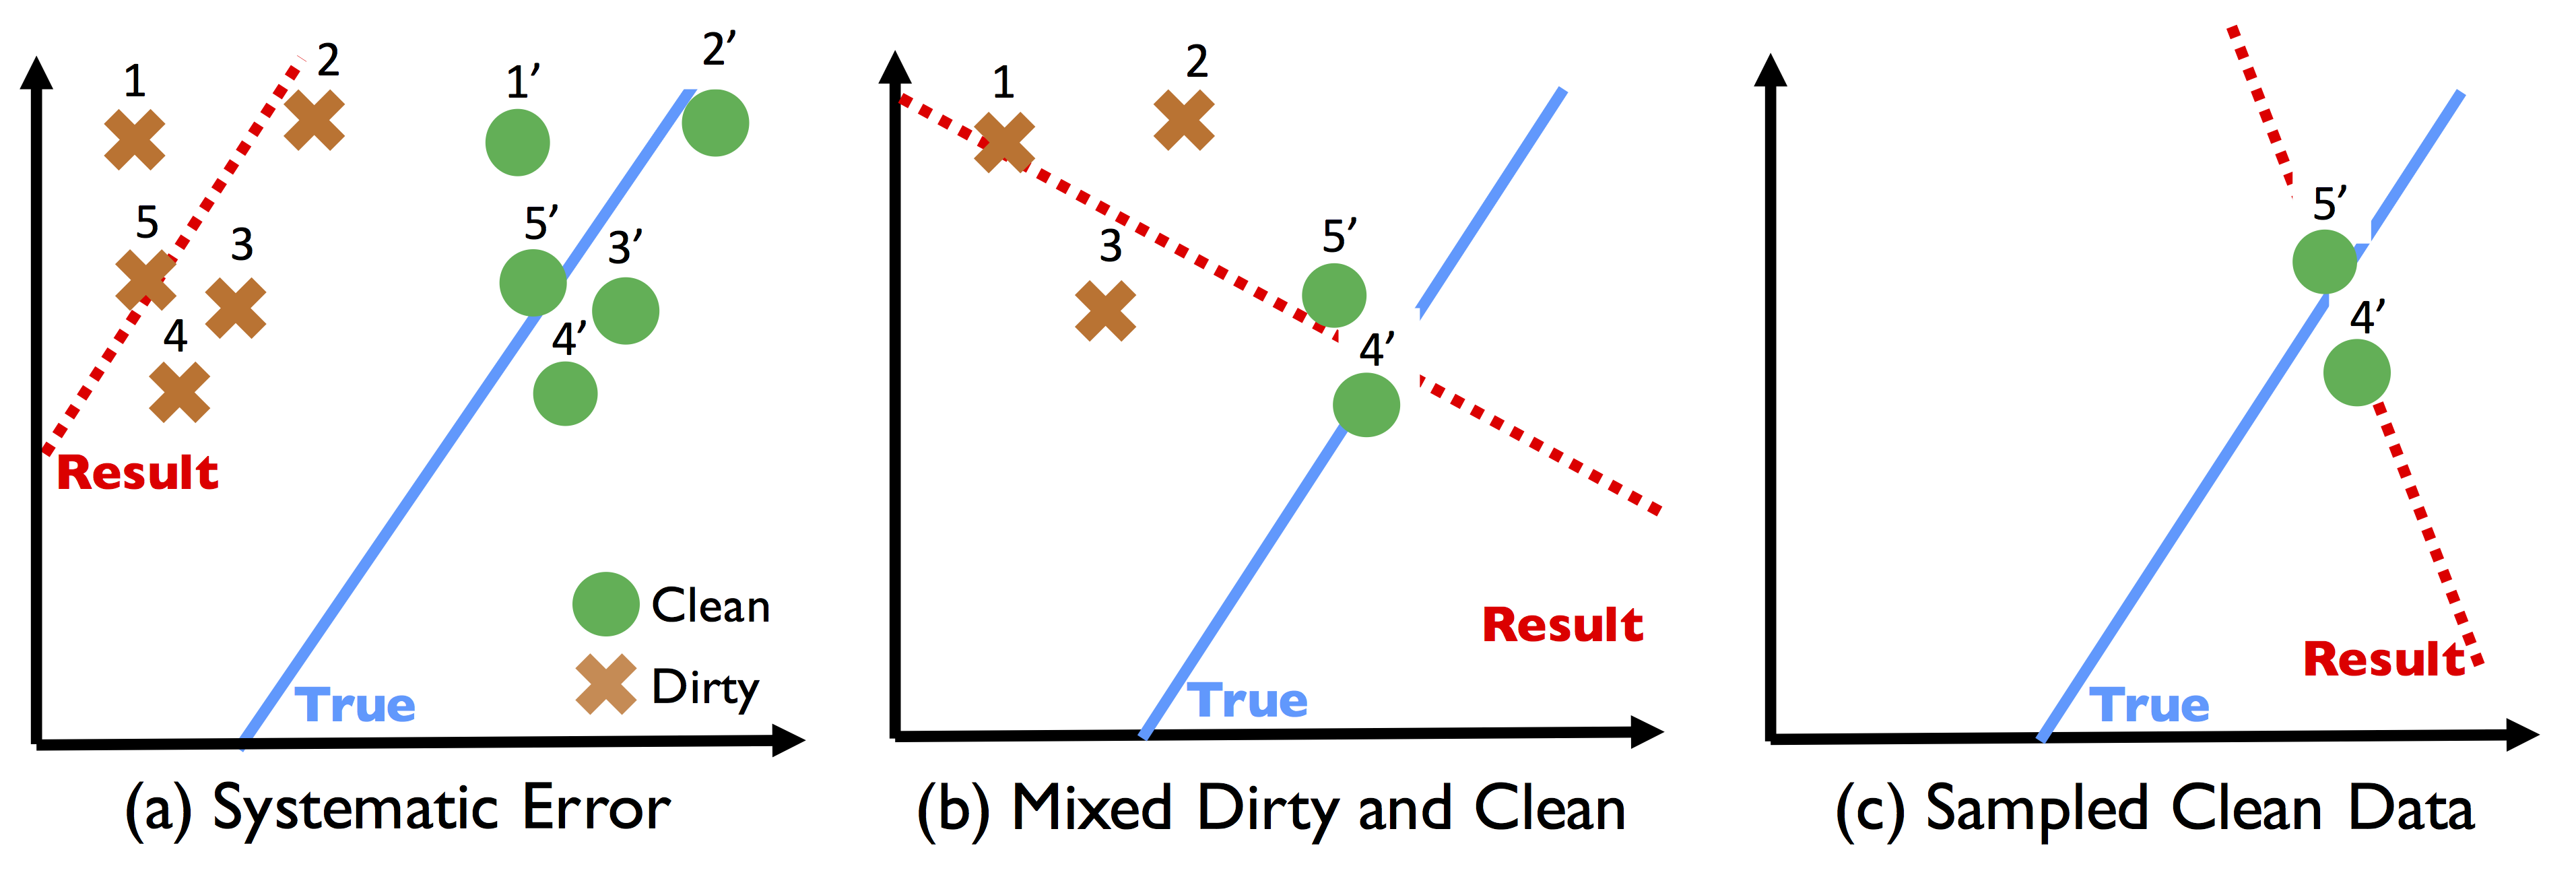
\includegraphics[width=\columnwidth]{figs/update-arch.png}
 \caption{(a) Systematic corruption in one variable can lead to a shifted model. The dirty examples are labeled 1-5 and the cleaned examples are labeled 1'-5'. 
 (b) Mixed dirty and clean data results in a less accurate model than no cleaning.
(c) Small samples of only clean data can result in similarly inaccurate models. \label{update-arch-coverletter}}
\end{figure}

\vspace{0.5em}

\noindent\textbf{R1.8 End of Sec 2.1. Why regularization term does not affect the results? It was stated w/o justification.}

\noindent We have revised the paper to make this clearer.
None of the results that we present in this paper depend on the regularization term $r(\theta)$.
Consider the regularized convex-loss minimization problem:
\[
 \theta^{*}=\arg\min_{\theta}\sum_{i=1}^{N}\phi(x_{i},y_{i},\theta) + r(\theta)
\]
Since $r(\theta)$ does not depend on on $i$, we can move it into the sum and treat is as part of $\phi$.

\vspace{0.5em}

\noindent\textbf{R1.9 Example 1 assumes very small sample (50). Why? Is that only for illustration purpose?}

\noindent   The numbers in the examples (budgets, etc.) are chosen for illustration purposes. In the particular example, each iteration samples a batch of 50 records to clean.  A discussion is included in Section \ref{sgd} on how that value can be set depending on the application:

\vspace{0.5em}
\emph{The batch size should be set by the user to have the desired properties.
Larger batches will take longer to clean and will make more progress towards the clean model but will have less frequent model updates.
On the other hand, smaller batches are cleaned faster and have more frequent model updates.}

\vspace{0.5em}

For example, if the data cleaning is implemented using crowdsourcing, then larger batches can be used. Alternatively, if the data cleaning is implemented via manual action, then smaller batches may be used.
The batch size does affect the rate of convergence, and we discuss this in Section \ref{sgd} as well. 

\vspace{0.5em}

\noindent\textbf{R1.10 Sec 4.2. Steps 4-5 need more intuition}

\noindent  Section 4.2 is Section 4.3 in the revision. We have clarified that Step 4 ``is a weighted average of the gradient on the already clean data and newly cleaned data", and Step 5 ``appends the newly cleaned data to set of previously clean records''.

\vspace{0.5em}

\noindent\textbf{R1.11 End of Sec 5. Expected Gradient Length heuristic needs more explanation}

\noindent  The discussion about Expected Gradient Length was an effort to analogize our work with Active Learning, because both are iterative algorithms. This was a side point that made the text more confusing, and we have removed it.
Section \ref{dist-samp} provides a detailed discussion of the sampling problem, what the optimal solution is, and how we apply an approximation to the optimal.

\subsection*{Review 2 Details}

\noindent\textbf{R2.1: Although the problem (iterative data cleaning) is novel, the techniques themselves are quite similar to active learning techniques.}

\noindent  We have included a revised discussion on the differences with Active Learning:

\emph{ The motivation of \sys similar to that of Active Learning~\cite{DBLP:journals/pvldb/YakoutENOI11,gokhale2014corleone} as both seek to reduce the number of queries to an analyst or a crowd.
However, Active Learning addresses a fundamentally different problem than \sys.
Active Learning poses the problem of iteratively selecting the most informative {\it unlabeled} examples to label in partially labeled datasets---these
examples are labeled by an expert and integrated into the machine learning model.
Note that Active Learning does not handle cases where the dataset is labelled incorrectly.
In contrast, \sys studies the problem of prioritizing modifications to both features and labels in existing examples.
In essence, \sys handles incorrect values in {\it any} part (label or feature) of an example.
This property fundamentally changes the type of analysis and algorithms that can be used.}

\vspace{0.5em}

\noindent\textbf{R2.2: The selection of the records to clean in each iteration (efficiency problem) uses heuristic solutions (e.g., expected gradient length). There is no formal study of the efficiency of the solution.}

\noindent  We have expanded the technical discussion of the prioritization solution and a number of experiments that evaluate its efficiency. Section \ref{dist-samp} formally describes the optimal sampling problem and our solution to it which is an approximation to the optimum. We clearly note that the \sys will converge for any sampling distribution where there is non-zero sampling probability for all remaining dirty records--and more accurate approximations only lead to faster convergence. In all of our experiments, we include ActiveClean + Oracle, which is the theoretical best performance with an optimal sampler and optimal detector.
Our results suggest that the approximate solution is very competitive to the optimum. 

 \subsection*{Reviewer 3}

\noindent\textbf{R3.1 The background sections were not very clear. This needs to be improved
to make this accessible to a general audience.}

\noindent  We have revised the background section to make the problem clearer. The background section first introduces a use case and the problems with existing tools, and then transitions to the formalism. We also significantly expanded the discussion about the system architecture~(Section \ref{syarch}), which provides intuition on the key insights.

\vspace{0.5em}

\noindent\textbf{R3.2 The jump to sampling over dirty data (Section 5.2) was too abrupt.
I do not understand statistics well enough to see why this will work at all,
and the statistically correct updates argument. Also see D6.}

\noindent  We have made several revisions to clarify the relationship between updating, sampling, and detection. We expanded the architecture section to overview the main data flows and an example of how an analyst may use \sys~(Section \ref{syarch}). Section \ref{det} now formalizes the detection component and presents our solution, and Section~\ref{dist-samp} formalizes the sampling problem and then presents our solution.

The main insight of \sys is to model the interactive data cleaning process as a form of Stochastic Gradient Descent (SGD)~\cite{bottou2012stochastic}.
SGD is an iterative optimization algorithm that starts with an initial estimate and then takes a sequence of steps ``downhill'' to minimize an objective function.
Similarly, in interactive data cleaning, the human starts with a dirty model and makes a series of cleaning decisions to improve the accuracy of the model.
We formalize the link between these two processes, and since SGD is one of the most widely studied forms of optimization, it is well understood theoretical convergence conditions.


\vspace{0.5em}

\noindent \textbf{R3.3 I was confused by Identify() in Section 2.4.
From the pseudocode, it appears Identify is picking from R,
those rows that are mispredicted under current\_model.
But why should these be the only rows that are Clean()d.
I thought cleaning was an operation that can
affect both rows that are mispredicted and rows that
are predicted correctly. Update() is not defined.}

\noindent  We have removed the pseudo-code in favor of a more precise discussion of the system architecture in Section \ref{syarch}. This new section highlights all of the components, the key data flows, and their conditions for correctness. 
The cleaning operation is applied to all rows in a batch whether or not they are predicted correctly.
In each iteration, \sys suggests a batch of data to clean based on the value to the model and the likelihood that the rows are actually dirty.

\vspace{0.5em}

\noindent \textbf{R3.4. Suppose k much less than N .. are retained .. Aren't all
the dirty records cleaned?}

\noindent This section discusses the correctness of the intermediate result (before the data are fully cleaned).
We meant to say that the user-defined cleaning function $C()$ was only applied to $k$ records.

\vspace{0.5em}

\noindent\textbf{R3.5. Sentence not clear - ' We have access to dirty
values may give us ..'}

 \noindent We have revised this to make it clear (see R2.1).

\vspace{0.5em}

\noindent\textbf{R3.6. It is not clear where R\_dirty is initialized. Do yu start with R\_dirty -= R? Or is it the set of rows misclassified in the 1st iteration?}

\noindent Section \ref{syarch} now describes the initialization as follows:

\emph{ We first initialize $R_{dirty} = R$ and $R_{clean} = \emptyset$.
The system first trains the model on $R_{dirty}$ to find an initial model $\theta^{(d)}$ that the system will subsequently improve iteratively.}

\vspace{0.5em}

\noindent\textbf{R3.7. The apriori detector assumption seems bogus.} 

\noindent  We have revised the detector section to clarify what we meant by the ``a priori'' detector (Section \ref{rule-det}). This section explains how we can integrate \emph{a priori} knowledge about which records are known to be dirty. We apologize for the lack of clarity and we have now renamed it a ``rule-based detector'' and have described concrete scenarios to which it applies. 

\vspace{0.5em}

\emph{In the data cleaning literature, error detection and error repair are treated as two distinct problems~\cite{DBLP:series/synthesis/2012Fan, Dasu:2003:EDM:861869, rahm2000data}.
Error detection is often considered to be substantially easier than error repair since one can declare a set of integrity rules on a database (e.g., an attribute must not be NULL), and select rows that violate those rules.
On the other hand, repair is harder and often requires human involvement (e.g., imputing a value for the NULL attribute).}

\vspace{0.5em}

\emph{Data quality rules are widely studied as a technique for detecting data errors.
In most rule-based frameworks, an analyst declares a set of rules $\Sigma$ and checks whether a relation $R$ satisfies those rules. The rules rules can be declared in advance before applying \sys, or constructed from the first batch of sampled data.
\sys is compatible with many commonly used classes of rules for error detection including integrity constraints (ICs), conditional functional dependencies (CFDs), and matching dependencies (MDs).
The only requirement on the rules is that there is an algorithm to enumerate the set of records that violate at least one rule.}

%\title{ActiveClean: Progressive Data Cleaning For Convex Data Analytics}
\title{ActiveClean: Interactive Data Cleaning \\ For Statistical Modeling}

\numberofauthors{1}
\author{ Sanjay Krishnan, Jiannan Wang{$\,^{\dag}$}, Eugene Wu{$\,^{\dag\dag}$}, Michael J. Franklin, Ken Goldberg \\
\affaddr{ UC Berkeley, ~~ $^\dag$Simon Fraser University, ~~ $^{\dag\dag}$Columbia University} \\
\affaddr{ \{sanjaykrishnan, franklin, goldberg\}@berkeley.edu ~~ jnwang@sfu.ca ~~ ewu@cs.columbia.edu}\\
%\affaddr{}
}

%\fontsize{9pt}{11pt}
%\selectfont


\maketitle

\begin{abstract}
Analysts often clean dirty data iteratively--cleaning some data, executing the analysis, and then cleaning more data based on the results.
We explore the iterative cleaning process in the context of statistical model training, which is an increasingly popular form of data analytics.  
We propose \sys, which allows for progressive and iterative cleaning in statistical modeling problems while preserving convergence guarantees.
\sys supports an important class of models called convex loss models (e.g., linear regression and SVMs), and prioritizes cleaning those records likely to affect the results.
We evaluate \sys on five real-world datasets UCI Adult, UCI EEG, MNIST, IMDB, and Dollars For Docs with both real and synthetic errors.
The results show that our proposed optimizations can improve model accuracy by up-to 2.5x for the same amount of data cleaned.
Furthermore for a fixed cleaning budget and on all real dirty datasets, \sys returns more accurate models than uniform sampling and Active Learning. 
\end{abstract}

\if{0}
\begin{abstract}
Databases are susceptible to various forms of corruption, or \emph{dirtiness}, such as missing, incorrect, or inconsistent values.
Increasingly, modern data analysis pipelines involve Machine Learning for predictive models which can be sensitive to dirty data.
Dirty data is often expensive to repair, and naive sampling solutions are not suited for training high dimensional models.
In this paper, we propose \sysfull, an anytime framework for training Machine Learning models with budgeted data cleaning.
Our framework updates a model iteratively as small samples of data are cleaned, and includes numerous optimizations such as importance weighting and dirty data detection.
We evaluate \sys on 4 real datasets and find that our methodology can return more accurate models for a smaller cost  than alternatives such as uniform sampling and active learning.
\end{abstract}
\fi

\setcounter{page}{1}
\setcounter{figure}{0}


\section{Introduction}\label{intro}
Statistical models trained on historical data facilitate several important predictive applications such as fraud detection, recommendation systems, and automatic content classification.
In a survey of Apache Spark users, over 60\% responded that support for advanced statistical analytics was Spark's most important feature~\cite{sparksurvey}.
This sentiment is echoed across both industry and academia, and there has been significant interest in improving the efficiency of model training pipelines. 
Although it is often overlooked, an important step in all model training pipelines is handling dirty or inconsistent data including extracting structure, imputing missing values, and handling incorrect data.
Analysts widely report that cleaning dirty data is a major concern~\cite{kandel2012}, and consequently, it is important to understand the efficiency and correctness of such operations in the context of emerging statistical analytics.

While many aspects of the data cleaning problem have been well-studied for SQL analytics, the results can be counter-intuitive in high-dimensional statistical models.
For example, studies have shown that many analysts do not approach cleaning as a one-shot pre-processing step, and instead, repeatedly alternate between cleaning and analysis.
It is common to use the preliminary analysis on dirty data as a guide to help identify potential errors and design repairs~\cite{fayyad1996data, kandel2012,krishnan2016hilda}.
Unfortunately, for statistical models, iteratively cleaning some data and re-training on a partially clean dataset can lead to biases in even the simplest models.

\begin{figure}[t]
\centering
 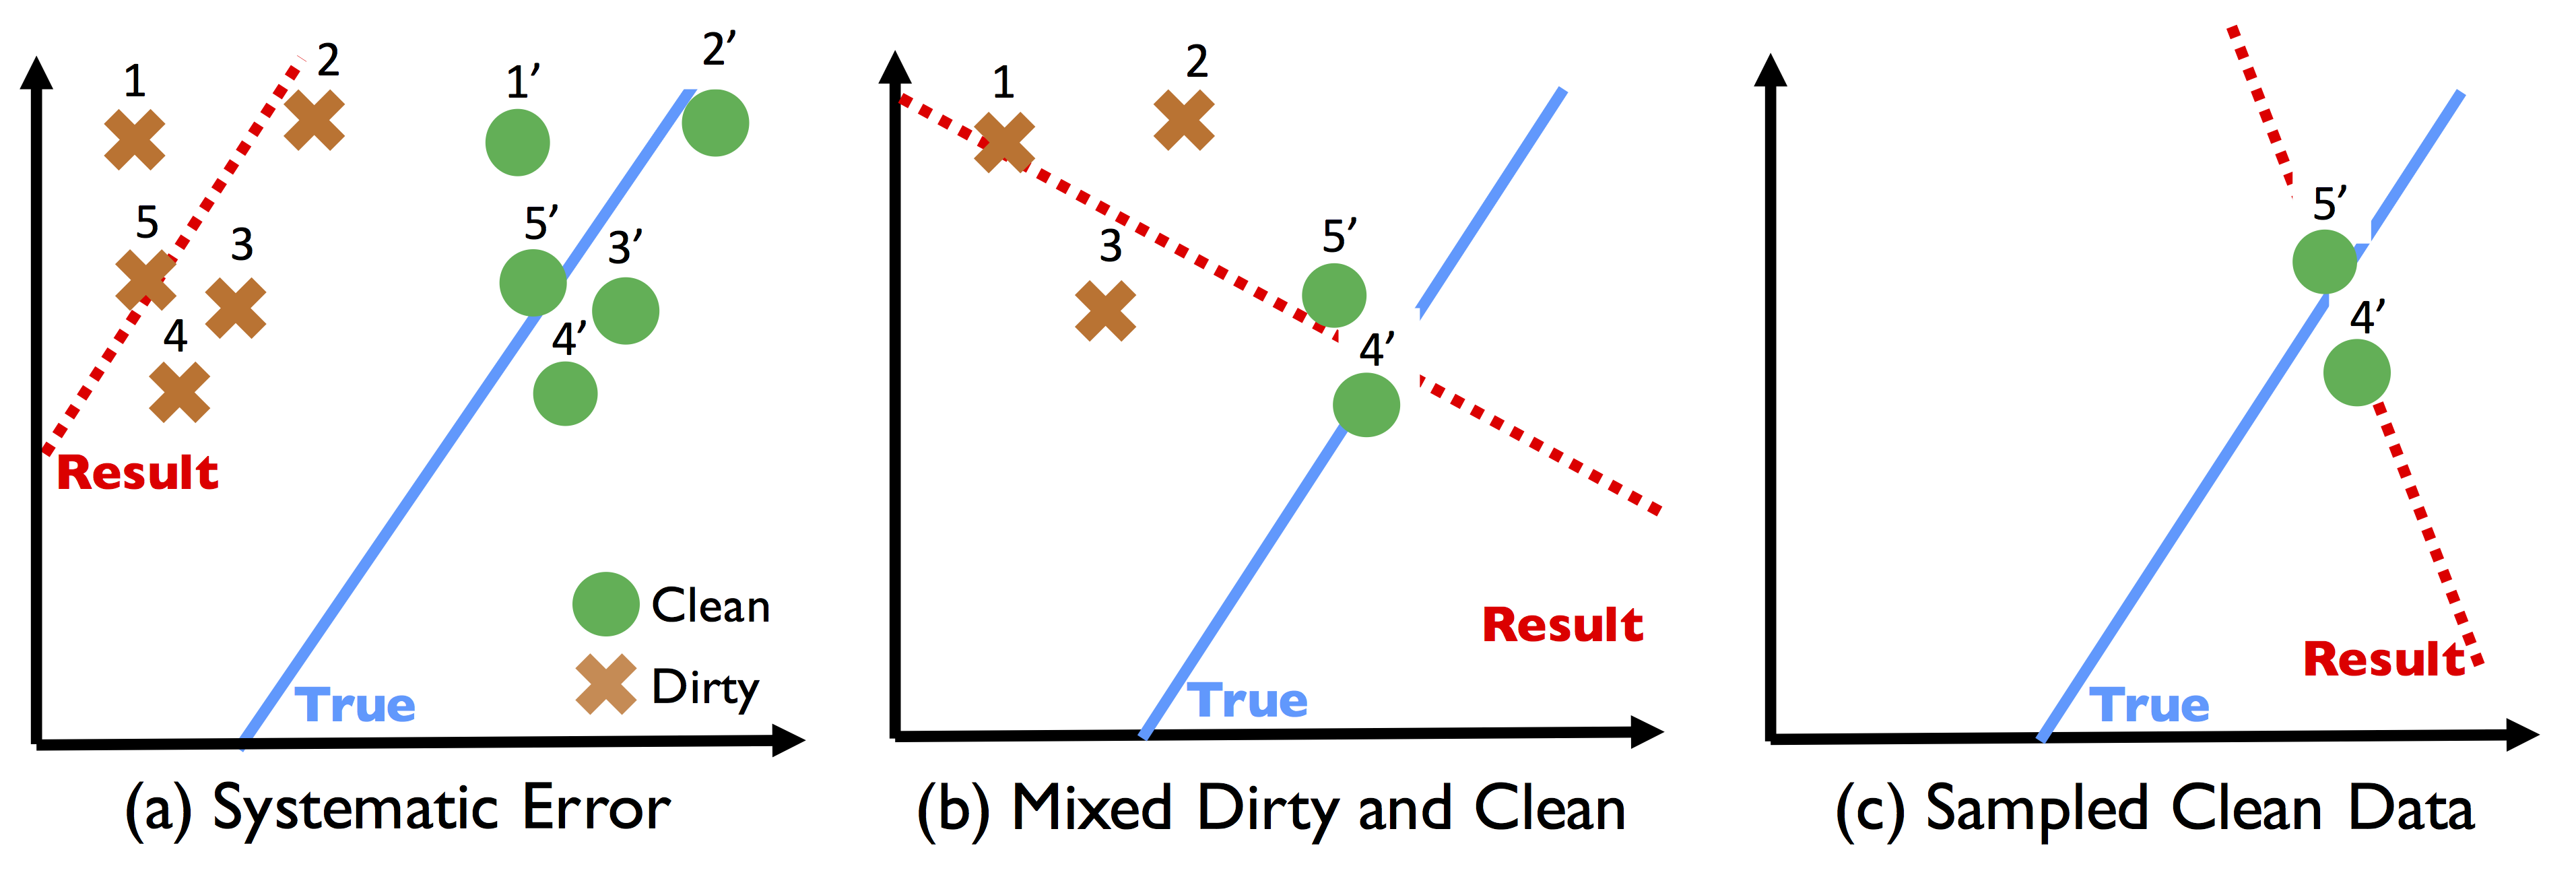
\includegraphics[width=\columnwidth]{figs/update-arch.png}
 \caption{(a) Systematic corruption in one variable can lead to a shifted model. The dirty examples are labeled 1-5 and the cleaned examples are labeled 1'-5'.
 (b) Mixed dirty and clean data results in a less accurate model than no cleaning.
(c) Small samples of only clean data can result in similarly issues. \label{update-arch1}}\vspace{-1em}
\end{figure}

Consider a linear regression model on systematically translated data (Figure \ref{update-arch1}a).
If one only cleans two of the data points, the intermediate result reveals a misleading trend (Figure \ref{update-arch1}b).
This is a consequence of the well-known Simpson's paradox where aggregates over different populations of data can result in spurious relationships~\cite{simpson1951interpretation}. 
Similarly, statistical models face more dramatic sampling effects than the traditional 1D  \sumfunc, \countfunc, \avgfunc SQL aggregates (Figure \ref{update-arch1}c).
The challenges with Simpson's paradox and sampling are problematic because recent advances in SQL data cleaning, such as Sample-and-Clean~\cite{wang1999sample} and Progressive Data Cleaning~\cite{altowim2014progressive, papenbrock2015progressive, DBLP:journals/pvldb/YakoutENOI11}, actually advocate cleaning subsets of data to avoid the potentially expensive cleaning costs.
Clearly, such data cleaning approaches will have to be re-evaluated for the statistical modeling setting, and this paper explores how to adapt such approaches with guarantees of convergence for an important class of modeling problems. 

Data cleaning is a broad area that encompasses extraction, de-duplication, schema matching, and many other problems in relational data.
We focus on two common operations that often require iterative cleaning: removing outliers and attribute transformation.
For example, battery-powered sensors can transmit inaccurate measurements when battery levels are low \cite{DBLP:conf/pervasive/JefferyAFHW06}. 
Similarly, data entered by humans can be susceptible to a variety of inconsistencies (e.g., typos), and unintentional cognitive biases~\cite{DBLP:conf/recsys/KrishnanPFG14}.
Since these two types of errors do not affect the schema or leave any obvious signs of corruption (e.g., NULL values), model training may seemingly succeed--albeit with an inaccurate result.

We propose \sys, a model training framework that allows for iterative data cleaning while preserving provable convergence properties.
The analyst initializes \sys with a model, a featurization function, and a pointer to a dirty relational table.
In each iteration, \sys suggests a sample of data to clean based on the data's value to the model and the likelihood that it is actually dirty.
The analyst can apply value transformations and filtering operations to the sample. 
\sys will incrementally and safely update the current model (as opposed to complete re-training).
We propose several novel optimizations that leverage information from the model to guide data cleaning towards the records most likely to be dirty and most likely to affect the results.
%\sys can also incorporate prior knowledge about records that are likely to be dirty.

From a statistical perspective, our key insight is to treat the cleaning and training iteration as a form of Stochastic Gradient Descent, an iterative optimization method.
We treat the dirty model as an initialization, and incrementally take gradient steps (cleaning a sample of records) towards the global solution (i.e., the clean model).
Our algorithm ensures global convergence with a provable rate for an important class of models called \emph{convex}-loss models which include SVMs, Linear Regression, and Logistic Regression.
Convexity is a property that ensures that the iterative optimization converges to a true global optimum, and we can apply convergence arguments from convex optimization theory to show that \sys converges.

To summarize our contributions:
\begin{itemize}[noitemsep]
\item We propose \sys, which allows for progressive data cleaning and statistical model training with guarantees.
\item \textbf{Correctness} We show how to update a dirty model given newly cleaned data. This update converges monotonically in expectation with a with rate $O(\frac{1}{\sqrt{T}})$.
\item \textbf{Optimizations} We derive a theoretically optimal sampling distribution that minimizes the update error and an approximation to estimate the theoretical optimum. We further show that \sys can integrate with existing dirty data detection techniques. Our proposed optimizations can improve model accuracy by up-to 2.5x for the same amount of data cleaned.
\item \textbf{Experiments} The experiments evaluate \sys on five datasets with real and synthetic corruption. In a fraud prediction example, \sys examines nearly 10x less records than alternatives to achieve an 80\% true positive rate.
\end{itemize}
The correctness of many of the components detailed proofs, which we have included in our extended technical report~\cite{activecleanarxiv}.






\section{Iterative Data Cleaning}\label{background}
This section introduces the problem of iterative data cleaning through an example application.

\subsection{Use Case: Dollars for Docs}\label{s:usecase}
ProPublica collected a dataset of corporate donations to medical researchers to analyze conflicts of interest~\cite{dollarsfordocsa}. 
For reference, the dataset has the following schema:
{\ssmall\begin{verbatim}
Contribution(
 pi_specialty text, # PI's medical specialty
 drug_nm text ,  # drug brand name, null if not drug
 device_nm text, # device brand name, null if not a device
 corp text,      # name of pharamceutical donor
 amount float,   # amount donated
 dispute bool,   # whether the research is disputed
 status text     # if the donation is allowed 
                 # under research protocol
)
\end{verbatim}
}

\vspace{1.5em}

% \begin{lstlisting}[mathescape,basicstyle={\small}]
% Contribution(pi_specialty$\textrm{,}$ drug_name$\textrm{,}$ device_name$\textrm{,}$
% $~~~~~~~~~~~~~~~~~~~~~~~~~~~~~~~$corporation$\textrm{,}$ amount$\textrm{,}$ dispute$\textrm{,}$ status)
% \end{lstlisting}
% 
% \noindent\texttt{pi\_specialty:} textual attribute describing the specialty of the doctor receiving the donation.
% 
% \noindent\texttt{drug\_name:} branded name of the drug in the research study (null if not a drug).
% 
% \noindent\texttt{device\_name} is the branded name of the device in the study (null if not a device).
% 
% \noindent\texttt{corporation} is the name of the pharmaceutical providing the donation.
% 
% \noindent\texttt{amount} is a numerical attribute representing the donation amount.
% 
% \noindent\texttt{dispute} is a Boolean attribute describing whether the research was disputed.
% 
% \noindent\texttt{status} is a string label describing whether the  donation was allowed under the declared research protocol. The goal is to predict disallowed  donation. 



%Some of these donations are flagged as suspicious after careful manual review.
%We collected the raw data and explored whether suspect donations could be predicted with an Support Vector Machine model.

The dataset comes with a \texttt{status} field that describes whether or not the donation was allowed under the declared research protocol.
Unfortunately the dataset is dirty, and there are inconsistent ways to specify ``allowed'' or ``disallowed''.
The ProPublica team identified the suspicious donations via extensive manual review (documented in ~\cite{dollarsfordocs}).
However, new donation datasets are continuously released and would need to be analyzed by hand.
Thus, let us consider an alternative ActiveClean-based approach to train a model to predict the true \texttt{status} value.
This is necessary for several reasons: 1) training a model on the raw data would not work because the \texttt{status} field is often inconsistent and incorrect;
2) techniques such as active learning are only designed for acquiring {\it new} labels and not suitable for finding and fixing {\it incorrect} labels;
and 3) other attributes such as company name may also be inconsistent (e.g., Pfizer Inc., Pfizer Incorporated, Pfizer) and need to be canonicalized before they are useful
for training the model.
%This problem is typical of analysis scenarios based on observational data seen in finance, insurance, medicine, and investigative journalism.

During our analysis, we found that nearly 40,000 of the 250,000 records had some form of inconsistency.
Indeed, these errors were structural rather than random---disallowed donations were more likely to have an incorrect \texttt{status} value.
In addition, larger pharmaceutical comparies were more likely to have inconsistent names, and more likely to make disallowed donations.
Without cleaning company names, a model would miss-predict many large pharmaceutical donations.
In fact, we found that the true positive rate for predicting disallowed donations when training an SVM model on the raw data was only 66\%.
In contrast, cleaning the entire dataset improves this rate to 97\% (Section \ref{exp:dfd}), and we show in the experiments that ActiveClean
can achieve comparable model accuracy (< 1\% of the true model accuracy) while expending only 10\% of the data cleaning effort.
The rest of this section will introduce the key challenges in designing a Machine-Learning-oriented iterative data cleaning framework.



% Suppose instead that we train a classification model to predict the \texttt{status} field of a donation, which can be used to focus manual analysis efforts in the future.
% Unfortunately, errors in the rest of the dataset make training such a model difficult.  this dataset contains numerous errors that needed to be cleaned before publication
% %and in the Technical Report~\cite{activecleanarxiv}).
% For example, company names were often inconsistently represented in the data, e.g., Pfizer Inc., Pfizer Incorporated, Pfizer.
% A crucial data cleaning operation is to canonicalize these various names.
% \reminder{Why would duplicates reduce correlation?  How does that affect propublica/svm?}.
% Duplicate representations could artificially reduce the correlation between certain companies and suspected contributions.
% Furthermore, donation records were often inconsistently flagged, e.g. Suspicious, Review, Disallowed.
% Nearly 40,000 of the 250,000 records had some form of inconsistency.
% 
% When we analyzed this data, we found that the errors were indeed structural and not random.  %were not random and were correlated with the eventual prediction.
% First, records that were suspicious were more likely to have an inconsistent flagging attribute.
% Next, the names of the larger pharmaceutical companies were also more likely to have inconsistent names, and it turns out that these companies were also more likely to provide a flagged donation.
% Without data cleaning, the true positive rate of an SVM model is only 66\%.
% Applying the data cleaning to the entire dataset improved this rate to 97\% in the clean data (Section \ref{exp:dfd}).
% This problem is typical of analysis scenarios based on observational data seen in finance, insurance, medicine, and investigative journalism.
% 

\iffalse
\begin{figure}[t]
\centering
 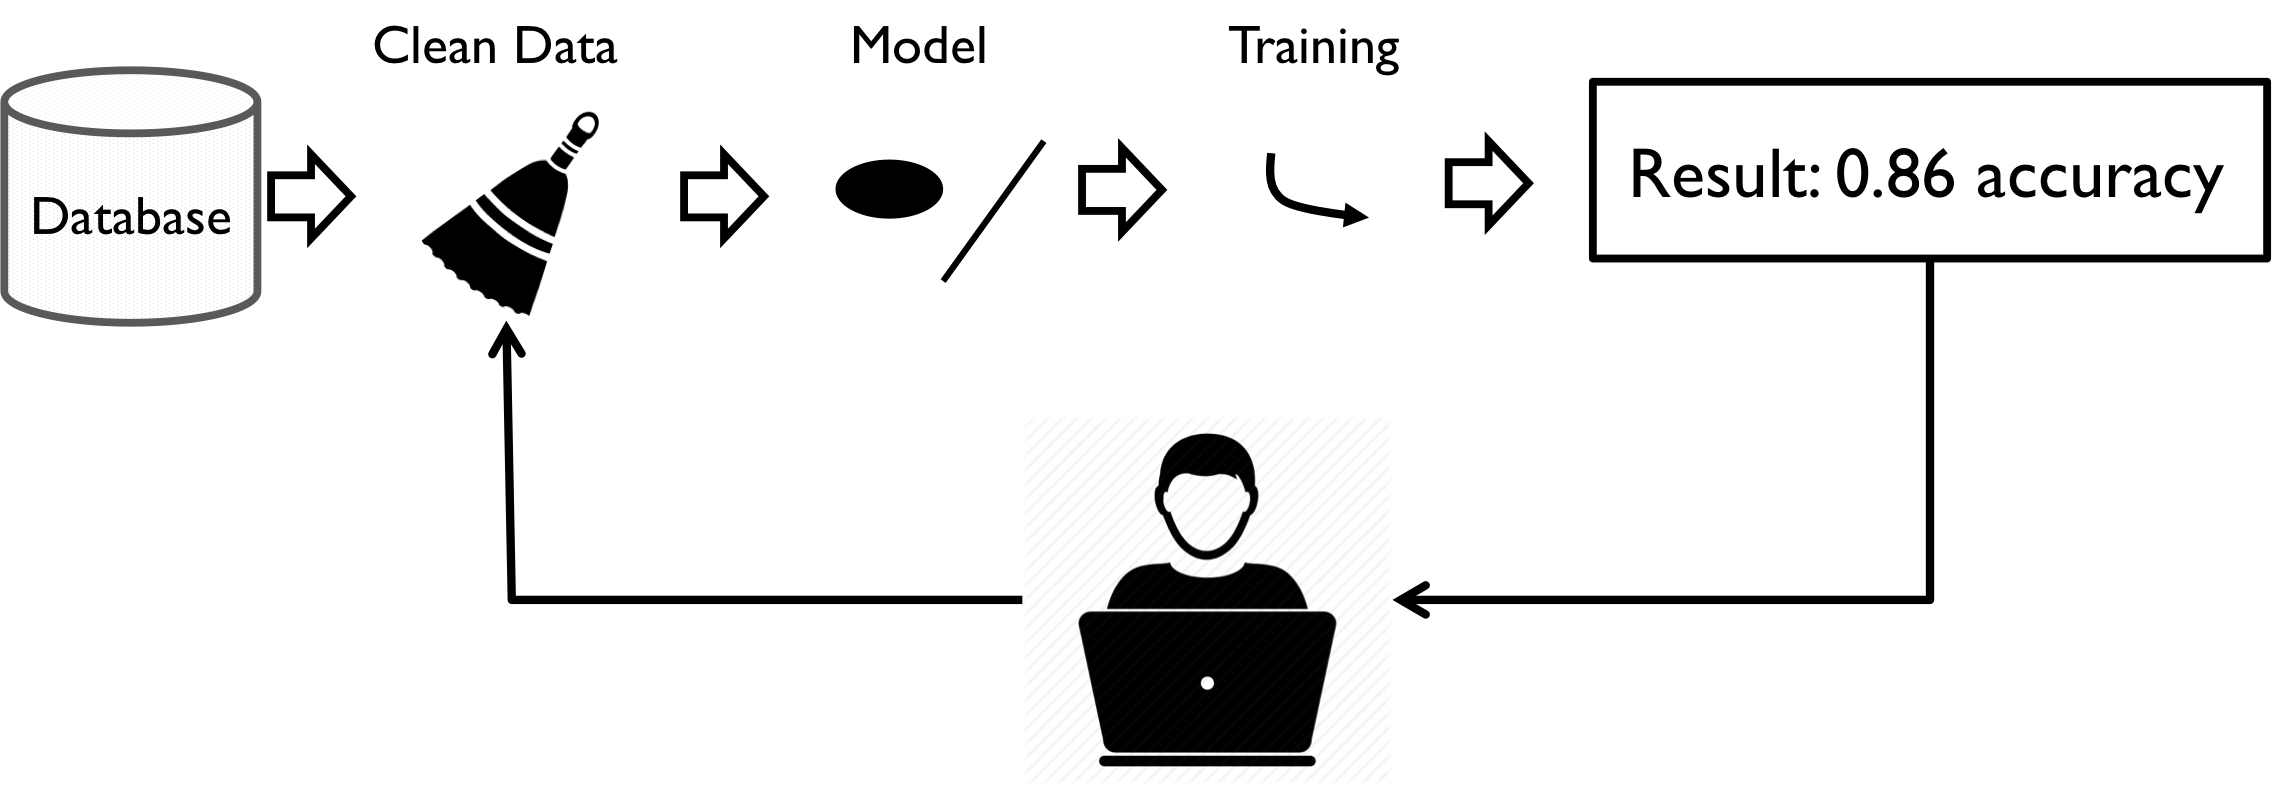
\includegraphics[width=0.8\columnwidth]{figs/workflow.png}
 \caption{Analysts often clean data interactively with data analytics; iteratively cleaning some data and re-training on a partially clean dataset to evaluate whether the cleaning was effective. It is common to use the preliminary analysis on dirty data as a guide to help identify potential errors and design repairs. \label{cartoon}}
\end{figure}
\fi

\subsection{Iteration in Model Construction}\label{alcmp}
Consider an analyst designing a classifier for this dataset.
When she first develops her model on the dirty data, she will find that the detection rate (true positives predicted) is quite low 66\%.
To investigate why she might examine those records that are incorrectly predicted by the classifier.

It is common for analysts to use the preliminary analysis on dirty data as a guide to help identify potential errors and design repairs~\cite{kandel2012}.
For example, our analyst may discover that there are numerous examples where two records are nearly identical, but one is predicted correctly, and one is incorrect, and their only difference is the \texttt{corporation} attribute: Pfizer and Pfizer Incorporated.
Upon discovering such inconsistencies, she will merge those two attribute values, re-train the model, and repeat this process.

We define iterative data cleaning to be the process of cleaning subsets of data, evaluating preliminary results, and then cleaning more data as necessary.
\sys explores two key questions about this iterative process: (1) \emph{Correctness.} Will this clean-retrain loop converge to the intended result and (2) \emph{Efficiency.} How can we best make use of the existing data and analyst effort.

\vspace{0.5em}
\noindent \textbf{Correctness: } The straight-forward application of data cleaning is to repair the corruption in-place, and re-train the model after each repair.
However, this process has a crucial flaw, where a model is trained on a mix of clean and dirty data.
It is known that aggregates over mixtures of different populations of data can result in spurious relationships due to the well-known phenomenon called Simpson's paradox \cite{simpson1951interpretation}.
Simpson's paradox is by no means a corner case, and it has affected the validity of a number of high-profile studies~\cite{pearl2003causality}.
Figure \ref{update-arch1} illustrates a simple example where such a process can lead to unreliable results, where artificial trends introduced by the mixture can be confused for the effects of data cleaning.
The consequence is that after applying a data cleaning operation on a subset of data the analyst cannot be sure if it makes the model more or less accurate.
\sys provides an update algorithm with a monotone convergence guarantee where more cleaning is leads to a more accurate result in expectation.

\vspace{0.5em}
\noindent \textbf{Efficiency: } One could alternatively avoid the mixing problem by taking a small sample of data up-front, perfectly cleaning it, and then training a model.
This approach is similar to SampleClean \cite{wang1999sample}, which was proposed to approximate the results of aggregate queries by applying them to a clean sample of data.
However, high-dimensional models are highly sensitive to sample size, and it is not uncommon to have models whose training data complexity is exponential in the dimensionality (i.e., the curse of dimensionality).
Figure \ref{update-arch1}c illustrates that, even in two dimensions, models trained from small samples can be as incorrect as the mixing solution described before.
Sampling further has a problem of scarcity, where errors that are rare may not show up in the sample.
\emph{\sys uses a model trained on the dirty data as an initialization and uses this model as guide to identify future data to clean.}

\vspace{0.5em}
\noindent \textbf{Comparison to Active Learning: } The motivation of \sys similar to that of Active Learning~\cite{DBLP:journals/pvldb/YakoutENOI11,gokhale2014corleone} as both seek to reduce the number of queries to an analyst or a crowd.
However, active learning addresses a fundamentally different problem than \sys.
Active Learning poses the problem of iteratively selecting the most informative {\it unlabeled} examples to label in partially labeled datasets---these
examples are labeled by an expert and integrated into the machine learning model.
Note that active learning does not handle cases where the dataset is labelled incorrectly but only cases where labels are missing.
In contrast, \sys studies the problem of prioritizing modifications to both features and labels in existing examples.
In essence, \sys handles incorrect values in {\it any} part (label or feature) of an example.
This property changes the type of analysis and algorithms that can be used.
Consequently, our experiments find that general active learning approaches (e.g., uncertainty sampling~\cite{settles2010active}) converge slower than \sys. 
If the only form of data error was missing labels, then we would expect active learning to perform comparably or better than \sys.

%This would be like Active Learning, where instead of unlabled data, there are inaccurate prior estimates for the labels.
%\sys reduces to a form of Expected Gradient Length Active Learning when there is no structure in the dirty data to exploit (such as completely missing attribute values).





\section{Problem Formalization}\label{statements}
\sys is an iterative framework for cleaning data in support of statistical modeling.
Analysts clean batches of data, which are fed back into the system to intelligently re-train the model, and recommend a next batch of data to clean.
We will first introduce the terms used in the rest of the paper, describe our assumptions, and define the two problems that we solve in this paper.

\subsection{Assumptions}\label{dmodel}
In this paper, we use the term \emph{statistical modeling} to describe a well-studied class of analytics problems; ones that can be expressed as the minimization of convex loss functions.
Examples include linear models (including linear and logistic regression), support vector machines, and in fact, means and medians are also special cases. 
This class is restricted to supervised Machine Learning, and the result of the minimization is a vector of parameters $\theta$.
We further assume that there is a one-to-one mapping between records in a relation $R$ and labeled training examples $(x_{i},y_{i})$.

\sys considers data cleaning operations that are applied record-by-record.
That is, the data cleaning can be represented as a user-defined function $C(\cdot)$ that when applied to a record $r$ and can perform two actions: recover a unique clean record $r' = C(r)$ with the same schema or remove the record $\emptyset = C(r)$.
\sys is agnostic to how $C(\cdot)$ is implemented, e.g., with software or a manual action by the analyst.
We define the clean relation as a relation of all of the records after cleaning:
\[R_{clean} = \cup_i^N C(r_i \in R)\]
Therefore, for every $r' \in R_{clean}$ there exists a unique $r \in R$ in the dirty data.
Supported cleaning operations include merging common inconsistencies (e.g., merging ``U.S.A" and ``United States"), filtering outliers (e.g., removing records with values $>1e6$), and standardizing attribute semantics (e.g., ``1.2 miles" and ``1.93 km").
Our technical report discusses a generalization of this basic data cleaning model called the ``set of records" cleaning model~\cite{activecleanarxiv}.
In this generalization, the $C(\cdot)$ function is composed of schema preserving \textsf{map} and \textsf{filter} operations applied to the entire dataset.
This can model problems such batch merging of inconsistencies with a ``find-and-replace".
We acknowledge that both definitions of data cleaning are limited as they do \emph{not} cover errors that simultaneously affect multiple records such as record duplication or structure such as schema transformation.

\subsection{Notation}\label{notation}
The user provides a pointer to a dirty relation $R$, a cleaner $C(\cdot)$, a featurizer $F(\cdot)$, and a convex loss problem.
A total of $k$ records will be cleaned in batches of size $b$, so there will be $T = \frac{k}{b}$ iterations of the algorithm.  
We use the following notation to represent relevant quantities:

\vspace{0.25em}

\noindent\textbf{Dirty Model: } $\theta^{(d)}$ is the model trained on $R$ (without cleaning). 

\vspace{0.25em}

\noindent\textbf{Dirty Records: } $R_{dirty} \subseteq R$ is the subset of records that are still dirty. As more data are cleaned $R_{dirty} \rightarrow \{\}$.

\vspace{0.25em}

\noindent\textbf{Clean Records: } $R_{clean} \subseteq R$ is the subset of records that are clean, i.e., the complement of $R_{dirty}$.

\vspace{0.25em}

\noindent\textbf{Batches: } $S$ is a batch of data (possibly selected stochastically but with known probabilities) from the records $R_{dirty}$. The clean batch is denoted by $S_{clean} = C(S)$.

\vspace{0.25em}

\noindent\textbf{Clean Model: } $\theta^{(c)}$ is the optimal clean model, i.e., the model trained on a fully cleaned relation. Accuracy and convergence are always with respect to $\theta^{(c)}$.

\noindent\textbf{Current Model: } $\theta^{(t)}$ is the current best model at iteration $t \in \{1,...,\frac{k}{b}\}$, and $\theta^{(0)} = \theta^{(d)}$. 


\subsection{System Architecture}\label{syarch}
The main insight of \sys is to model the interactive data cleaning problem as Stochastic Gradient Descent (SGD)~\cite{bottou2012stochastic}.
SGD is an iterative optimization algorithm that starts with an initial estimate and then takes a sequence of steps ``downhill'' to minimize an objective function.
Similarly, in interactive data cleaning, the human starts with a dirty model and makes a series of cleaning decisions to improve the accuracy of the model.
We formalize the link between these two processes, and since SGD is one of the most widely studied forms of optimization, it has well understood theoretical convergence conditions.
These theoretical properties give us clear restrictions on different components.
Figure \ref{sys-arch} illustrates the \sys architecture including the: {\it Sampler}, {\it Cleaner}, \emph{Updater}, {\it Detector}, and {\it Estimator}.

The first step of \sys is initialization. We first initialize $R_{dirty} = R$ and $R_{clean} = \emptyset$.
The system first trains the model on $R_{dirty}$ to find an initial model $\theta^{(d)}$ that the system will subsequently improve iteratively.
It turns out that SGD converges for an arbitrary initialization, so $\theta^{(d)}$ need not be very accurate. 
This can be done by featurizing the dirty records (e.g., using an arbitrary placeholder for missing values), and then training the model.

In the next step, the {\it Sampler} selects a batch of data $S$ from the data that has not been cleaned already. To ensure convergence, the Sampler has to do this in a randomized way, but can assign higher probabilities to some data as long as no data has a zero sampling probability.
The {\it Cleaner} is user-specified and executes $C(\cdot)$ for each sample record and outputs their cleaned versions.
The {\it Updater} uses the cleaned batch to update the model using a Gradient Descent step, thus moving the model closer to the true cleaned model (in expectation).
Finally, the system either terminates due to a stopping condition (e.g., $C(\cdot)$ has been called a maximum number of times $k$, or training error convergence), or passes control to the {\it sampler} for the next iteration.

A user provided {\it Detector} can be used to identify records that are more likely to be dirty (e.g., using data quality rules), and thus improves the likelihood that the next sample will contain true dirty records. Furthermore, the {\it Estimator} uses previously cleaned data to estimate the effect that cleaning a given record will have on the model. These components are optional, but our experiments show that these optimizations can improve model accuracy by up-to 2.5x (Section \ref{comp}).

\begin{figure}[t]
\centering
 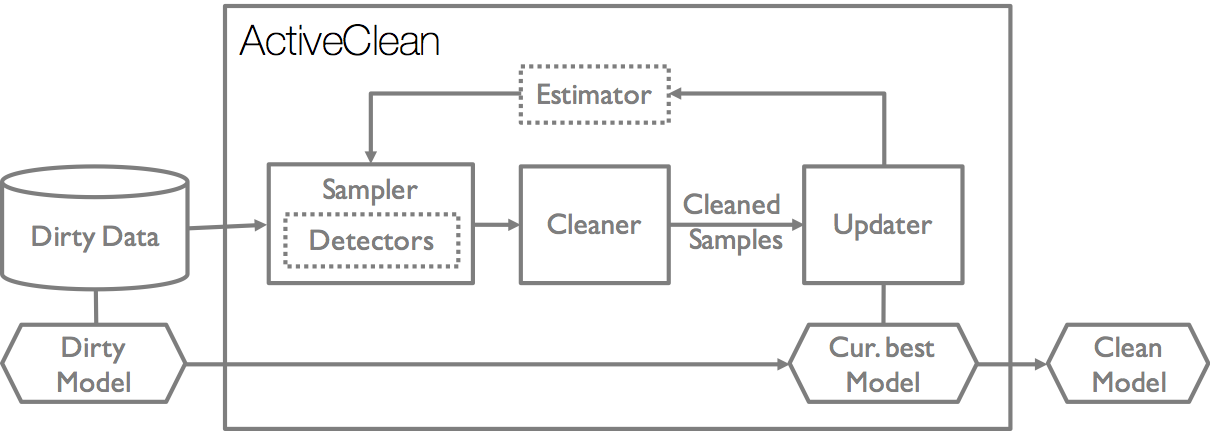
\includegraphics[width=0.8\columnwidth]{figs/arch.png}
 \caption{\sysfull allows users to train predictive models while progressively cleaning data but preserves convergence guarantees. Solid boxes are essential components for correctness and 
 dotted boxes indicate optimizations that can improve model accuracy by up-to 2.5x (Section \ref{comp}) \label{sys-arch}}
\end{figure}

Going back to the ProPublica example in Section~\ref{s:usecase}:
\begin{example}\label{archex}
The analyst chooses to use an SVM model, and manually cleans records by hand (the $C(\cdot)$).  
\sys initially selects a sample of $50$ records (the default) to show the analyst.
She identifies records that are dirty, fixes them by normalizing the drug and corporation names with the help of a search engine, and corrects the labels with typographical or incorrect values.
The system then uses the cleaned records to update the current best model and selects the next sample of $50$.
The analyst can stop at any time and use the improved model to predict whether a record is fraudulent or not.
\end{example}

\subsection{Problem Statements}\label{updp}

\vspace{0.5em}

\noindent\textbf{Update Problem: } Given a newly cleaned batch of data $S_{clean}$ and the current best model $\theta^{(t)}$, the model update problem is to calculate $\theta^{(t+1)}$. 
$\theta^{(t+1)}$ will have some error with respect to the true model $\theta^{(c)}$, which we denote as:
\[
error(\theta^{(t+1)}) = \| \theta^{(t+1)} - \theta^{(c)} \|
\]
The Update Problem is to update the model with a monotone convergence guarantee such that more cleaning implies a more accurate model.

Since the sample is potentially stochastic, it is only meaningful to talk about expected errors.
Formally, we require that the expected error is upper bounded by a monotonically decreasing function $\mu$ of the amount of cleaned data:
\[
\mathbb{E}(error(\theta^{new})) = O(\mu(\mid S_{clean} \mid))
\]
%Intuitively, ``reliable" means that more cleaning should imply more accuracy.

\vspace{0.5em}

\noindent\textbf{Prioritization Problem: } The prioritization problem is to select $S_{clean}$ in such a way that the model converges in the fewest iterations possible. 
Formally, in each batch of data, every $r$ has a probability $p(r)$ of being included.
The Prioritization Problem is to select a sampling distribution $p(\cdot)$ to maximize the progress made which each iteration of the update algorithm.
We derive the optimal sampling distribution for the updates, and show how the theoretical optimum can be approximated, while still preserving convergence.




\iffalse

\subsection{\sys Problem}
The core problem addressed by \sys is incremental model update while progressively cleaning data.

\begin{problem}[ActiveClean Problem]\label{activeclean}\sloppy
Let $R$ be a dirty relation, $F(r) \mapsto (x,y)$ be a featurization that maps
a record $r \in R$ to a feature vector $x$ and label $y$, $\phi$ be a convex regularized loss,
and $C(r) \mapsto r_{clean}$ be a cleaning technique that maps a record to its cleaned value. 
Given these inputs, the \sys problem is to return a \textbf{reliable} estimate $\hat{\theta}$ of the clean model for any limit $k$ on the number of times the data cleaning $C(\cdot)$ can be applied.

\vspace{0.5em}

\textbf{Reliable} precisely means that the expected error in this estimate (i.e., L2 difference w.r.t a model trained on a fully cleaned dataset) is bounded above by a monotonic function in $k$ and a monotonic function of the error in the dirty model.
\end{problem}
\fi


\iffalse
From a systems perspective, data cleaning and model training happen at very different time scales.
When humans are involved, per record latencies for data cleaning are orders of magnitude larger than the CPU time needed for model training.
We can compare recent results in data cleaning to a model training framework like CoCoA implemented on Spark \cite{jaggi2014communication}.
Per record, BigDansing, a highly optimized automated Spark-based data cleaning system is 15.5x slower than CoCoA\footnote{For CoCoA to reach a precision of 1e-3}.
Crowd based techniques like CrowdFill \cite{park2014crowdfill} and CrowdER \cite{wang2012crowder} are over 100,000x slower per record. 
Consequently, all of the optimizations in \sys are designed to address data cleaning latency (i.e., more progress with fewer cleaned records) rather than optimizing for numerical computation (i.e., process fewer records).
\fi



\iffalse
Here is an example application of \sys with our running example:
\begin{example}
The analyst first trains her SVM model on the dirty data ignoring the effects of the errors returning a model $\theta^{(d)}$.
She decides that she has a budget of cleaning $100$ records, and decides to clean the 100 records in batches of 10 (set based on how fast she can clean the data, and how often she wants to see an updated result).
She initializes \sys with $\theta^{(d)}$.
\sys samples an initial batch of 10 records.
She manually cleans those records by merging similar drug names, making corporation names consistent, and fixing incorrect labels.
After each batch, the model is updated with the most recent cleaning results $\theta^{(t)}$.
The model improves after each iteration.
After $t=10$ of cleaning, the analyst has an accurate model trained with 100 cleaned records but still utilizes the entire dirty data.
\end{example}



\subsection{Two perspectives on error}
When faced with such errors there are two contrasting perspectives from the Machine Learning and the Database communities.

\vspace{0.5em}

\noindent\textbf{Existing Database Literature. } 
Traditionally, cleaning is agnostic to the queries and analysis that happens downstream. 
This perspective breaks down when cleaning is so expensive that we can only clean a small number of records.
Ideally, we should clean the records that are most valuable to the downstream analysis.

\vspace{0.5em}

\noindent\textbf{Existing  Machine Learning Literature. } The Machine Learning community has focused on
designing models that are robust to outliers (i.e., values far away from the typical value)
For example, in the case of linear regression, we can change the $L_2$ norm to an $L_1$ norm to mitigate the effect of outliers:
\[
\phi(x_{i}^T\theta,y_{i}) = \|\theta^Tx_{i} - y_i \|_1
\]
The quadratic L2 loss implies that examples that deviate far from the typical example are quadratically penalized as opposed to linearly penalized with the L1 loss.
There is a natural tradeoff between robustness and efficiency.
The more robust a technique is, the less efficient it will be (i.e., estimate variance for a fixed number of training examples).
Robust techniques are best suited for random errors that look significantly different the rest of the examples.
When errors are systematic, the Machine Learning answer has been to design features in such a way that they are robust to some systematic bias.
For example, in image processing, scale-invariant feature transforms (SIFT) are widely applied that allow for image models invariant to pose or scaling issues.

\vspace{0.5em}

\noindent\textbf{The \sys Contribution. } We try to bring two perspectives together in this work to address the problem of expensive to clean systematic errors, namely the Database idea of data cleaning and the Machine Learning formalization of empirical risk minimization.
Some errors require expensive cleaning procedures, increasingly using the crowd, and we joint have a time budget on cleaning and analysis.
\sys prioritizes cleaning with respect to an estimated impact on the clean model.

\subsection{SampleClean Project}

Traditionally, data cleaning has explored expensive, up-front cleaning of entire datasets for increased query accuracy.
We proposed the SampleClean problem, in which an analyst cleans a small sample of data, and then estimates the result to an aggregate query e.g., \sumfunc, \countfunc, or \avgfunc.
The main insight from the SampleClean project is that highly accurate answers for aggregate queries does not require cleaning the full dataset.
Generalizing this insight, there is a deep relationship between the application (i.e., the query) and how an analyst should budget their effort in data cleaning.
In fact, \avgfunc and \sumfunc queries are a special case of the convex loss minimization discussed in the previous section:
\[
\phi = (x_{i} - \theta)^2
\]

We then extended the SampleClean work to study cleaning Materialized Views \cite{technicalReport}.
Suppose base data is updated with insertions, deletions, or updates, we explored how we could efficiently propagate
changes to a sample of the view instead of the full view.
Subsequent queries on the view could be answered approximate.

The SampleClean problem inspired an eponymous system that implements sampling, data cleaning, and approximate query processing on the Apache Spark stack \cite{sampleclean}.
Also included in the Apache Spark stack are Machine Learning libraries including MLlib \cite{mllib} and GraphX \cite{graphx}.
The in-memory architecture of the Apache Spark stack allows for increasingly interactive analysis \cite{AgarwalMPMMS13, armbrust2015spark}.
Analysts can prototype data processing workflows on samples to evaluate performance before running expensive batch processing jobs on entire datasets.
With data cleaning and machine learning libraries in the same software ecosystem, we see a new opportunity for joint optimization for interactive model building.



\subsection{Stochastic Gradient Descent}
Sampling is a natural part of any Machine Learning workflow, as stochastic optimization is widely used to fit model parameters.
The problems described in the previous subsections are often trained using a technique called Stochastic Gradient Descent (SGD) or one of its variants.
The basic idea of SGD is to draw a data point at random, calculate the gradient at that point, and then update a current best estimate with that gradient.
\[
\theta^{(t+1)}\leftarrow\theta^{(t)}-\gamma\nabla\phi(x_{i}^T\theta,y_{i})
\]
 SGD can also be applied in a ``mini-batch" mode, where we draw a subset of data $S^{(t)}$ at random and update with the average gradient.
 \[
 \theta^{(t+1)}\leftarrow\theta^{(t)}-\frac{\gamma}{\|S^{(t)}\|}\sum_{i\in S^{(t)}}\nabla\phi(x_{i}^T\theta,y_{i})
 \]

We can use this workflow for designing an anytime data cleaning methodology.
As data is sampled, we can clean the samples.
The analyst then can stop at anytime and use the best model at that instant.
SGD and its variants are well-studied and there are lower-bounds on the convergence rates using these techniques. 
Recently, a number of works have explored non-uniform sampling distributions for stochastic optimization \cite{zhao2014stochastic, qu2014randomized}.
The main insight is that non-uniform distributions may on average estimate the gradient accurately.
In this work, we explore how to design such a non-uniform distribution for iterative data cleaning.

\fi


 

%\section{Architecture}\label{arch}
\noindent This section presents the \sys architecture.

\subsection{Overview}\label{sysover}
Figure \ref{sys-arch} illustrates the \sys architecture.
The dotted boxes describe optional components that the user can provide to improve the efficiency of the system.  

\subsubsection{Required User Input}\label{uinp}
%To use \sys, the user provides the following:

\noindent\textbf{Model:} The user provides a predictive model (e.g., SVM) specified as a convex loss optimization problem $\phi(\cdot)$ and a featurizer $F(\cdot)$ that maps a record to its feature vector $x$ and label $y$.

\vspace{0.25em}

\noindent\textbf{Cleaning Function: } The user provides a function $C(\cdot)$ (implemented via software or crowdsourcing) that maps dirty records to clean records as per our definition in Section \ref{dmodel}. 

\vspace{0.25em}

\noindent\textbf{Batches: } Data are cleaned in batches of size $b$ and the user can change these settings if she desires more or less frequent model updates.
The choice of $b$ does affect the convergence rate.
Section~\ref{model-update} discusses the efficiency and convergence trade-offs of different values of $b$.
We empirically find that a batch size of $50$ performs well across different datasets and use that as a default.
A cleaning budget $k$ can be used as a stopping criterion once $C(\dot)$ has been called $k$ times, and so the number of iterations of \sys is $T = \frac{k}{b}$.
Alternatively, the user can clean data until the model is of sufficient accuracy to make a decision.

\subsubsection{Basic Data Flow} \label{df}
The system first trains the model $\phi(\cdot)$ on the dirty dataset to find an initial model $\theta^{(d)}$ that the system will subsequently improve.
The {\it sampler} selects a sample of size $b$ records from the dataset and passes
the sample to the {\it cleaner}, which executes $C(\cdot)$ for each sample record and outputs their cleaned versions.
The \emph{updater} uses the cleaned sample to update the weights of the model, thus moving the model closer to the true cleaned model (in expectation).
Finally, the system either terminates due to a stopping condition (e.g., $C(\cdot)$ has been called a maximum number of times $k$, or training error convergence),
or passes control to the {\it sampler} for the next iteration.

In many cases, such as missing values, errors can be efficiently detected.
A user provided {\it Detector} can be used to identify such records that are more likely to be dirty, and thus improves the likelihood that the next sample will contain true dirty records.
Furthermore, the {\it Estimator} uses previously cleaned data to estimate the effect that cleaning a given record will have on the model.
These components can be used separately (if only one is supplied) or together to focus the system's cleaning efforts on records that will most improve the model.
Section \ref{opti} describes several instantiations of these components for different data cleaning problems.
Our experiments show that these optimizations can improve model accuracy by up-to 2.5x (Section \ref{comp}).

\subsection{Example}
The following example illustrates how a user would apply \sys to address the use case in Section~\ref{s:usecase}:
\begin{example}\label{archex}
The analyst chooses to use an SVM model, and manually cleans records by hand (the $C(\cdot)$).  
\sys initially selects a sample of $50$ records (the default)  to show the analyst.
She identifies a subset of 15 records that are dirty, fixes them by normalizing the drug and corporation names with the help of a search engine, and corrects the labels with typographical or incorrect values.
The system then uses the cleaned records to update the the current best model and select the next sample of $50$.
The analyst can stop at any time and use the improved model to predict donation likelihoods.
\end{example}






\iffalse
  \noindent To summarize in pseudocode:
  \begin{enumerate}[leftmargin=1em]\scriptsize\sloppy
  \item \texttt{Init(dirty\_data, cleaned\_data, dirty\_model, batch, iter)}
  \item For each t in $\{1,...,T\}$
  \begin{enumerate}
    \item \texttt{dirty\_sample $=$ sampler(dirty\_data, sample\_prob, detector, batch)}
    \item \texttt{clean\_sample $=$ Cleaner(dirty\_sample)}
    \item \texttt{current\_model $=$ Update(current\_model, sample\_prob, clean\_sample)}
    \item \texttt{cleaned\_data = cleaned\_data + clean\_sample}
    \item \texttt{dirty\_data = dirty\_data - clean\_sample}
    \item \texttt{sample\_prob $=$ Estimator(dirty\_data, cleaned\_data, detector)}
    \item \texttt{detector $=$ DetectorUpdater(detector, cleaned\_data)}
  \end{enumerate}
  \item \texttt{Output: current\_model}
  \end{enumerate}
\fi


\iffalse
  \subsection{Challenges and Formalization}
  We highlight the important components and formalize the research questions explored in this paper. 

  \vspace{0.5em}

  \noindent\textbf{Detector (Section \ref{det}). } The first challenge in \sys is dirty data detection. In this step, the detector selects a candidate set of dirty records $R_{dirty} \subseteq R$. There are two techniques to do this: (1) an \emph{a priori} case, and (2) and an adaptive case. In the \emph{a priori} case, the detector knows which data is dirty in advance. In the adaptive case, the detector learns classifier based on previously cleaned data to detect corruption in uncleaned data.

  \vspace{0.5em}



  \vspace{0.5em}



  \vspace{0.5em}

  \noindent\textbf{Update (Section \ref{model-update}). } This step updates the model $\theta^{(t)}$ based on the featurized (with featurization $F(\cdot)$) cleaned sample $F(S_{clean})$ resulting in $\theta^{(t+1)}$. Analyzing the model update procedure as a stochastic gradient descent algorithm will help derive the sampling distribution and estimation.

  \vspace{0.5em}

  \noindent\textbf{Estimator (Section \ref{sampling}): } The estimator approximates the optimal distribution derived in the Sample step. Based on the change in the featurized data $F(S_{clean})$ and $F(S_{dirty})$, it directs the next iteration of sampling to select points that will have changes most valuable to the next model update.


  \subsection{Optimizations}
  There are three aspects of \sys, that allow us to achieve this design point: error partitioning, gradient-based model update (Section \ref{model-update}), estimate-driven sampling (Section \ref{sampling}).

  \vspace{0.5em}

  \noindent\textbf{Partitioning Dirty and Clean Data: } In many applications, enumerating the set of corrupted records is much easier than cleaning them. For example, we may be able to select the set of rows that have missing values but actually filling those missing values is expensive. Likewise, in the constraint literature, selecting a set of rows that have a violated constraint can be done in polynomial time, however, fixing the constraints is NP-Hard.
  In our error detection step, we partition the dirty and clean data.
  Partitioning serves two purposes: (1) it reduces the variance of our updates because we can cheaply scan over data we know that is clean, and (2) it increases the fraction of actually dirty records in the candidate batch.
  A good example of why we need the second objective is seen in the context of crowdsourcing.
  If we have a crowdworker clean records, we will have to pay them for the task whether or not the record required cleaning.
  To efficiently use this partitioning, we need a database solution indexing dirty and clean data.

  \vspace{0.5em}

  \noindent\textbf{Gradient-Based Updates: } In \sys, we start with a dirty model and then make an update using a gradient step. Here, we can draw an analogy to Materialized View maintenance, since after all, a model parametrized by $\theta$ is just a table of floating point numbers.
  Krishnan et al. proposed a technique called sample view cleaning, in which they take a clean sample of data and propagate the updates to a Materialized View.
  Similarly, in this work, we take the information from a sample of cleaned data and propagate an update with the gradient.

  \vspace{0.5em}

  \noindent\textbf{Estimate-Driven Sampling: } Repair is the most expensive step in the workflow, so optimizing for scan cost may lead to negligible overall time improvements.
  We can sacrifice a small overhead in pre-computation for each data point to determine its value to the model and select a sampling distribution accordingly.
  Intuitively, while each iteration has an increased cost, it also makes more progress towards the optimum.


  \begin{example}

  The analyst first trains an SVM model on the dirty data ignoring the effects of the errors resulting in a model $\theta^{(d)}$.
  She decides that she has a budget of cleaning $100$ records, and decides to clean the 100 records in batches of 10 (set based on how fast she can clean the data, and how often she wants to see an updated result).
  She initializes \sys with $\theta^{(d)}$.
  \sys samples an initial batch of 10 records.
  She manually cleans those records by merging similar drug names, making corporation names consistent, and fixing incorrect labels.
  After each batch, the model is updated with the most recent cleaning results $\theta^{(t)}$.
  The model improves after each iteration.
  After $t=10$ of cleaning, the analyst has an accurate model trained with 100 cleaned records but still utilizes the entire dirty data.
  \end{example}
\fi

\begin{figure}[t]
\centering
 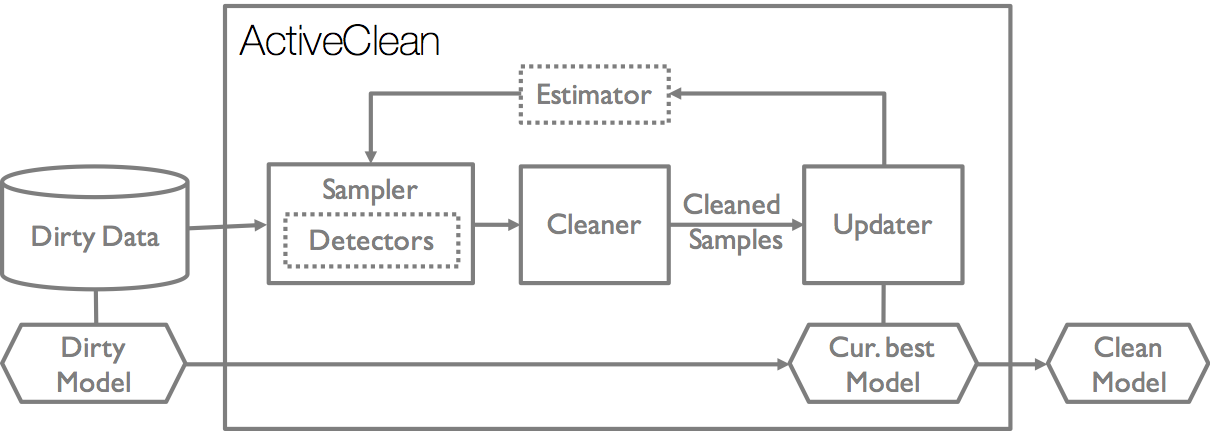
\includegraphics[width=\columnwidth]{figs/arch.png}
 \caption{\sysfull allows users to train predictive models while progressively cleaning data. The framework adaptively selects the best data to clean and can optionally (denoted with dotted lines) integrate with pre-defined detection rules and estimation algorithms for improved conference. \label{sys-arch}}
\end{figure}



\section{Updating the Model}\label{model-update}
This section describes an algorithm for reliable model updates.
For convex loss minimization, Stochastic Gradient Descent converges to an optimum from any initialization as long each gradient descent step is unbiased.
We show how we can leverage this property to prove convergence for interactive data cleaning regardless of the inaccuracy of the initial model--as long as the analyst does not systematically exclude certain data from cleaning. 
%To do so, we will sample yet-to-be-cleaned data in batches, where every record has a non-zero probability $p(i)$ of being sampled.
%Sections \ref{dist-samp} show how to select a non-uniform $p(\cdot)$ and the analysis in this section applies for any sampling distribution $p(\cdot) > 0$.
The updater only assumes that it is given a sample of data $S_{dirty}$ from $R_{dirty}$ where $i \in S_{dirty}$ has a known sampling probability $p(i)$.

\subsection{Convex Loss Models}
Formally, suppose $x$ is a feature vector and $y$ is a label.
For labeled training examples $\{(x_{i},y_{i})\}_{i=1}^{N}$, the problem is to find a vector of model parameters $\theta$ by minimizing a loss function $\phi$ (a function that measures prediction error) over all training examples:
\[
 \theta^{*}=\arg\min_{\theta}\sum_{i=1}^{N}\phi(x_{i},y_{i},\theta)
\]
where $\phi$ is a convex function in $\theta$.
For example, in a linear regression $\phi$ is:
\[
\phi(x_{i},y_{i},\theta) = \|\theta^Tx_{i} - y_i \|_2^2
\]
Sometimes, a convex \emph{regularization} term $r(\theta)$ is added to the loss:
\[
 \theta^{*}=\arg\min_{\theta}\sum_{i=1}^{N}\phi(x_{i},y_{i},\theta) + r(\theta)
\]
However, we ignore this term without loss of generality, since none of our results require analysis of the regularization.
The regularization can be moved into the sum as a part of $\phi$ for the purposes of this paper.

\subsection{Geometric Derivation}\label{geod}
The update algorithm intuitively follows from the convex geometry of the problem.
Consider the problem in one dimension (i.e., the parameter $\theta$ is a scalar value), so then the goal is to find the minimum point ($\theta$) of a curve $l(\theta)$.
The consequence of dirty data is that the wrong loss function is optimized.
Figure \ref{update-arch2}A illustrates the consequence of the optimization.
The red dotted line shows the loss function on the dirty data.
Optimizing the loss function finds $\theta^{(d)}$ at the minimum point (red star).
However, the true loss function (w.r.t to the clean data) is in blue, thus
the optimal value on the dirty data is in fact a suboptimal point on clean curve (red circle).

\begin{figure}[ht!]
\centering
 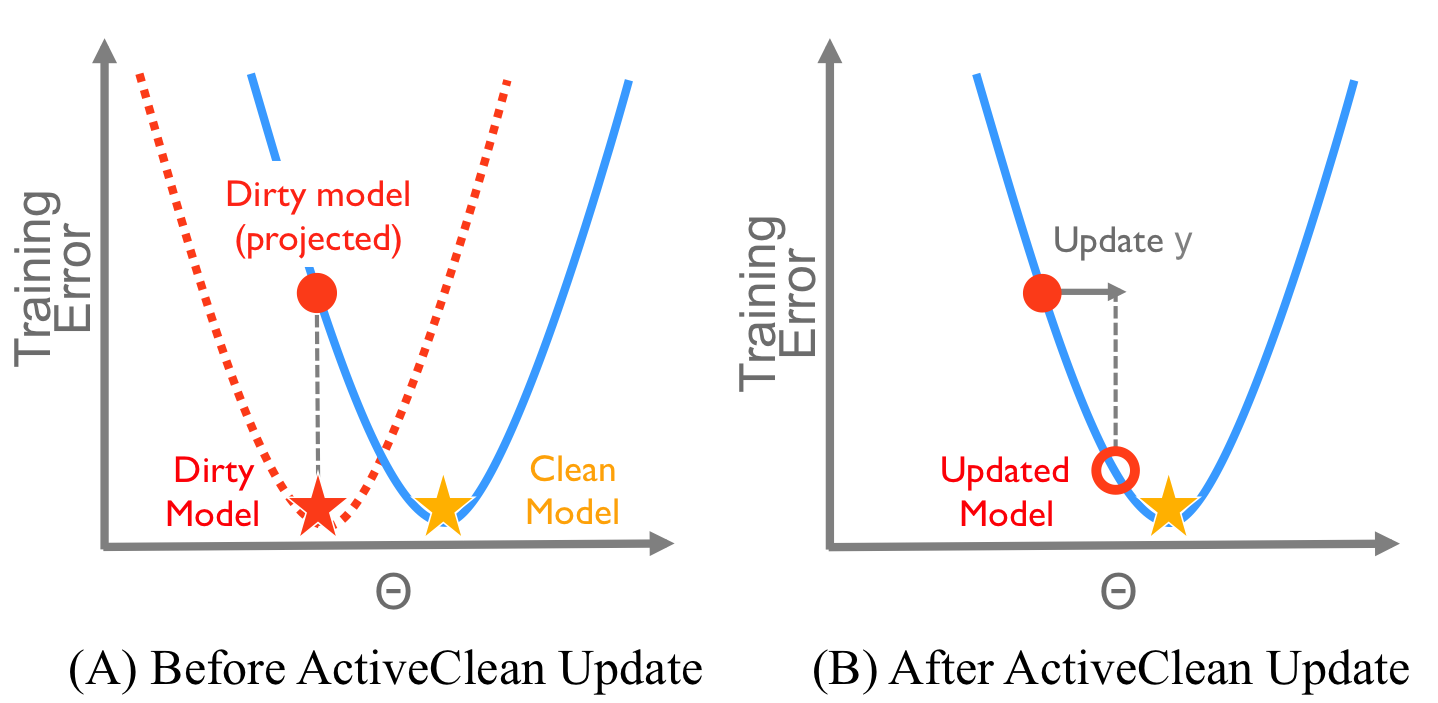
\includegraphics[width=0.8\columnwidth]{figs/update-arch2.png}
 \caption{(A) A model trained on dirty data can be thought of as a sub-optimal point w.r.t to the clean data. (B) The gradient gives us the direction to move the suboptimal model to approach the true optimum. \label{update-arch2}}
\end{figure}

In the figure, the optimal clean model $\theta^{(c)}$ is visualized as a yellow star.
The first question is which direction to update $\theta^{(d)}$ (i.e., left or right).
For this class of models, given a suboptimal point, the direction to 
the global optimum is the gradient of the loss function.
The gradient is a $p$-dimensional vector function of the current model $\theta^{(d)}$ and the clean data.
Therefore, \sys needs to update $\theta^{(d)}$ some distance $\gamma$ (Figure \ref{update-arch2}B):
\[
\theta^{new} \leftarrow \theta^{(d)} - \gamma \cdot \nabla\phi(\theta^{(d)})
\]
At the optimal point, the magnitude of the gradient will be zero.
So intuitively, this approach iteratively moves the model downhill (transparent red circle) -- correcting the dirty model until the desired accuracy is reached.
However, the gradient depends on all of the clean data, which is not available, and \sys will have to approximate the gradient from a sample of newly cleaned data.
%The main intuition is that if the gradient steps are on average correct, the model still moves downhill albeit with a reduced convergence rate proportional to the inaccuracy of the sample-based estimate.

To derive a sample-based update rule, the most important property is that sums commute with derivatives and gradients.
The convex loss class of models are sums of losses, so given the current best model $\theta$, the true gradient $g^*(\theta)$ is:
\[
g^*(\theta) = \nabla\phi(\theta) = \frac{1}{N} \sum_{i=1}^N \nabla\phi(x_i^{(c)},y_i^{(c)},\theta)
\]
\sys needs to estimate $g^*(\theta)$ from a sample $S$, which is drawn from the dirty data $R_{dirty}$.
 Therefore, the sum has two components which are the gradient from the already clean data $g_C$ and $g_S$ a gradient estimate from a sample of dirty data to be cleaned:
\begin{equation}
g(\theta) = \frac{\mid R_{clean} \mid}{\mid R \mid} \cdot g_C(\theta) + \frac{\mid R_{dirty} \mid}{\mid R \mid} \cdot g_S(\theta)\label{unbia}
\end{equation}
$g_C$ can be calculated by applying the gradient to all of the already cleaned records:
\[
g_C(\theta) = \frac{1}{\mid R_{clean}\mid}\sum_{i \in R_{clean}}\nabla\phi(x_i^{(c)},y_i^{(c)},\theta)
\] 
$g_S$ can be estimated from a sample by taking the gradient w.r.t each record, and re-weighting the average by their respective sampling probabilities.
Before taking the gradient, the cleaning function $C(\cdot)$ is applied to each sampled record.
Therefore, let $S$ be a sample of data, where each $i \in S$ is drawn with probability $p(i)$:
\[
g_{S}(\theta) = \frac{1}{\mid S \mid} \sum_{i \in S}\frac{1}{p(i)}\nabla\phi(x_i^{(c)},y_i^{(c)},\theta)
\]
Then, at each iteration $t$, the update becomes:
\[
\theta^{(t+1)} \leftarrow \theta^{(t)} - \gamma \cdot g(\theta^{(t)})
\]

\vspace{1em}

\subsection{Model Update Algorithm}\label{update-alg}
We present an outline for one iteration of the update algorithm.
To summarize, the algorithm is initialized with $\theta^{(0)} = \theta^{(d)}$ which is the dirty model.
There are three user set parameters: the budget $k$, batch size $b$, and the step size $\gamma$.
In the following section, we provide references from the convex optimization literature that allow the user to appropriately select these values.
At each iteration $t=\{1,...,T\}$, the cleaning is applied to a batch of data $b$ selected from the set of candidate dirty records $R_{dirty}$.
Then, an average gradient is estimated from the cleaned batch and the model is updated.
Iterations continue until $k = T \cdot b$ records are cleaned.

\vspace{1.5em}

\noindent The algorithm is as follows:
\begin{enumerate}[noitemsep]
	\item Take a sample of data $S$ from $R_{dirty}$ 
	\item Calculate the gradient over the sample of newly clean data and call the result $g_S(\theta^{(t)})$
	\item Calculate the average gradient over all of the already clean records in $R_{clean}=R-R_{dirty}$, and call the result $g_C(\theta^{(t)})$
	\item Apply the following update rule, which is a weighted average of the gradient on the already clean records and newly cleaned records:
	\[
	\theta^{(t+1)} \leftarrow \theta^{(t)} - \gamma \cdot(\frac{\mid R_{dirty} \mid}{\mid R \mid} \cdot g_S(\theta^{(t)}) + \frac{\mid R_{clean} \mid}{\mid R \mid} \cdot  g_C(\theta^{(t)}))
	\]
	\item Append the newly cleaned records to set of previously clean records $R_{clean} = R_{clean} \cup S$ 
\end{enumerate} 

This basic algorithm will serve as the scaffolding for the optimizations in the subsequent sections.
For example, if we know that a record is likely to be clean, we can move it from $R_{dirty}$ to $R_{clean}$ without having to sample it.
Similarly, we can set the sampling probabilities $p(\cdot)$ to favor records that are likely to affect the model.

\subsection{Analysis with Stochastic Gradient Descent}\label{sgd}
The update algorithm can be formalized as a class of very well studied algorithms called Stochastic Gradient Descent (SGD; more precisely the mini-batch variant of SGD).
In SGD, random subsets of data are selected at each iteration and the average gradient is computed for every batch.
The basic condition for convergence is that the gradient steps need to be on average correct.
We provided the intuition that this is the case in Equation \ref{unbia}, and this can be more rigorously formalized as an unbiased estimate of the true gradient~(see T.R \cite{activecleanarxiv}).
Then model is guaranteed to converge essentially with a rate proportional to the inaccuracy of the sample-based estimate.

One key difference with the tpyical application of SGD is that \sys takes a \emph{full} gradient step on the already clean data (i.e., not sampled) and averages it with a stochastic gradient step on the dirty data (i.e., sampled). 
This is because that data is already clean and we assume that the time-consuming step is the data cleaning and not the numerical operations.
The update algorithm can be thought of as a variant of SGD that lazily materializes the clean value.
As data is sampled at each iteration, data is cleaned when needed.
It is well-known that even for an arbitrary initialization, SGD makes significant progress in less than one epoch (a pass through the entire dataset) \cite{bottou2012stochastic}.
However, the dirty model can be much more accurate than an arbitrary initialization leading to even faster convergence.

\vspace{0.25em}

\noindent\textbf{ Setting the step size $\gamma$: } There is extensive literature in machine learning for choosing the step size $\gamma$ appropriately. $\gamma$ can be set either to be a constant or decayed over time. Many machine learning frameworks (e.g., MLLib, Sci-kit Learn, Vowpal Wabbit) automatically set this value. 
In the experiments, we use a technique called inverse scaling where there is a parameter $\gamma_0=0.1$, and at each iteration it decays to $\gamma_t = \frac{\gamma_0}{\mid S \mid t}$. 

\vspace{0.25em}

\noindent\textbf{ Setting the batch size $b$: } The batch size should be set by the user to have the desired properties.
Larger batches will take longer to clean and will make more progress towards the clean model but will have less frequent model updates.
On the other hand, smaller batches are cleaned faster and have more frequent model updates.
In the experiments, we use a batch size of 50 which converges fast but allows for frequent model updates.
If a data cleaning technique requires a larger batch size than 50, \sys can abstract this size away from the update algorithm and apply the updates in smaller batches.
For example, the batch size set by the user might be $b=1000$, but the model updates after every $50$ records are cleaned.
We can disassociate the batching requirements of SGD and the batching requirements of the data cleaning technique.

\vspace{0.25em}

\noindent\textbf{Convergence Conditions and Properties}
The convergence rates of SGD are also well analyzed \cite{dekel2012optimal,bertsekas2011incremental,zhao2014stochastic}. 
The analysis gives a bound on the error of intermediate models and the expected number of steps before achieving a model within a certain error. 
For a general convex loss, a batch size $b$, and $T$ iterations, the convergence rate is bounded by $O(\frac{\sigma^2}{\sqrt{bT}})$. 
$\sigma^2$ is a measure of how well the sample gradient estimates the gradient over the entire dataset, and $\sqrt{T}$ shows that each iteration has diminishing returns.
$\sigma^2$ is the variance in the estimate of the gradient at each iteration:
\[
\sigma^2 = \mathbb{E}(\|g - g^*\|^2)
\]
where $g^*$ is the gradient computed over the full data if it were fully cleaned.
This property of SGD allows us to bound the model error with a monotonically decreasing function of the number of records cleaned, thus satisfying the reliability condition in the problem statement.

Gradient descent techniques also can be applied to non-convex losses and they are widely used in graphical model inference and deep learning. In this case, however, instead of converging to a global optimum, they converge to a locally optimal value that dependends on the initialization.
In the non-convex setting, ActiveClean will converge to the closest locally optimal value to
the dirty model which is how we initialize \sys. Because of this, it is harder to reason about
the objective quality of the results and to define accuracy.
 Different initializations may lead to different local
optima, and thus, introduce a complex dependence on the
initialization with the dirty model.

\vspace{1.5em}

\begin{example}\label{upex}
Recall that the analyst has a dirty SVM model on the dirty data $\theta^{(d)}$.
She decides that she has a budget of cleaning $100$ records, and decides to clean the 100 records in batches of 10 (set based on how fast she can clean the data, and how often she wants to see an updated result).
All of the data is initially treated as dirty with $R_{dirty} = R$ and $R_{clean} = \emptyset$.
The gradient of a basic SVM is given by the following function:
\[
\nabla\phi(x,y,\theta) =
\begin{cases}      
-y\cdot\boldsymbol{x} ~~~~~~ \text{ if } y\boldsymbol{x}\cdot\theta < 1 \\
~~~~~~~0\ ~~~~~~\text{ if } y\boldsymbol{x}\cdot\theta \geq 1      
\end{cases}
\]

For each iteration $t$, a sample of 10 records $S$ is drawn from $R_{dirty}$.
\sys then applies the cleaning function to the sample.
Using these values, \sys estimates the gradient on the newly cleaned data:
\[
\frac{1}{10} \sum_{i \in S}\frac{1}{p(i)}\nabla\phi(x_i^{(c)},y_i^{(c)},\theta)
\]
\sys also applies the gradient to the already clean data (initially non-existent):
\[
\frac{1}{\mid R_{clean}\mid}\sum_{i \in R_{clean}}\nabla\phi(x_i^{(c)},y_i^{(c)},\theta)
\]
Then, it calculates the update rule:
\[
	\theta^{(t+1)} \leftarrow \theta^{(t)} - \gamma \cdot(\frac{\mid R_{dirty} \mid}{\mid R \mid} \cdot g_S(\theta^{(t)}) + \frac{\mid R_{clean} \mid}{\mid R \mid} \cdot  g_C(\theta^{(t)}))
\] 
Finally, $R_{dirty} \leftarrow R_{dirty} - S$, $R_{clean} \leftarrow R_{clean} + S$, and continue to the next iteration.
\end{example}

\vspace{2em}
\section{Dirty Data Detection}\label{det}
If corrupted records are relatively rare, sampling might be very inefficient.
The analyst may have to sample many batches of data before finding a corrupted record.
In this section, we describe how we can couple \sys with prior knowledge about which data are likely to be dirty.
In the data cleaning literature, error detection and error repair are treated as two distinct problems~\cite{DBLP:series/synthesis/2012Fan, Dasu:2003:EDM:861869, rahm2000data}.
 Error detection is often considered to be substantially easier than error repair since one can declare a set of integrity rules on a database (e.g., an attribute must not be NULL), and select rows that violate those rules.
On the other hand, repair is harder and often requires human involvement (e.g., imputing a value for the NULL attribute).

\subsection{Detection Problem}
First, we describe the required properties of the dirty data detector.
The detector returns two important aspects of a record: 
(1) whether the record is dirty, and (2) if it is dirty, on which attributes there are errors.
The sampler can use (1) to select a subset of dirty records to sample at each batch and 
the estimator can use (2) to estimate the value of data cleaning based on other records with the same corruption.

\begin{definition}[Detector]
Let $r$ be a record in $R$. A detector is a function that returns a Boolean of whether the record is dirty and a set of attributes $e_r$ that are dirty.
\[
D(r) = (\{0,1\}, e_r)
\]
\end{definition}

From the set of attributes that are dirty, we can find the corresponding features that are dirty $f_r$ and labels that are dirty $l_r$ since we assume a one-to-one mapping between records and training examples.
We will consider two types of detectors: exact rule-based detectors that detect integrity constraint or functional dependency violations, and approximate adaptive detectors that learn which data are likely to be dirty.

\subsection{Rule-Based Detector}\label{rule-det}
Data quality rules are widely studied as a technique for detecting data errors.
In most rule-based frameworks, an analyst declares a set of rules $\Sigma$ and checks whether a relation $R$ satisfies those rules.  The rules rules can be declared in advance before applying \sys, or constructed from the first batch of sampled data.
\sys is compatible with many commonly used classes of rules for error detection including integrity constraints (ICs), conditional functional dependencies (CFDs), and matching dependencies (MDs).
The only requirement on the rules is that there is an algorithm to enumerate the set of records that violate at least one rule.

Let $R_{viol}$ and $R_{sat}$ be the subset of records in $R_{ditry}$ that violate at least one rule and satisfy all rules respectively.
The rule-based detector modifies the update workflow in the following way:
\begin{enumerate}
\item $R_{clean} = R_{clean} \cup R_{sat}$
\item $R_{dirty} = R_{viol}$
\item Apply the algorithm in Section \ref{update-alg}.
\end{enumerate}

\begin{example}[Rule-Based Detection]\label{detex1}
An example of a rule on the running example dataset is that the \texttt{status} of
a contribution can be only ``allowed" or ``disallowed".
Any other value for \texttt{status} is considered violation.
\end{example}

\vspace{2em}

\subsection{Adaptive Detection}
Rule-based detection is not possible in all cases, especially in cases where the analyst selectively modifies data.
This is why we propose an alternative called the adaptive detector.
Essentially, we reduce the problem to training a classifier on previously cleaned data.
Note that this ``learning" is distinct from the ``learning" in the user-specified statistical model.
One challenge is that the detector needs to describe how the data is dirty.
The detector achieves this by categorizing the corruption into $u$ classes, and using a multi-class classifier.
These classes are corruption categories that do not necessarily align with features, but every record is classified with at most one category.

When using adaptive detection, the repair step has to clean the data and report to which of the $u$ classes the corrupted record belongs.
When an example $(x,y)$ is cleaned, the repair step labels it with one of the ${\text{clean}, 1,2,...,u}$.
It is possible that $u$ increases each iteration as more types of dirtiness are discovered.
In many real world datasets, data errors have locality, where similar records tend to be similarly corrupted.
There are usually a small number of error classes even if a large number of records are corrupted.
This problem can be addressed by any classifier, and we use an all-versus-one Logistic Regression in our experiments.

The adaptive detector modifies the update workflow in the following way:
\begin{enumerate}
\item Let $R_{clean}$ be the previously cleaned data, and let $U_{clean}$ be a set of labels for each record indicating the error class and if they are dirty or ``not dirty''.
\item Train a classifier to predict the label \textsf{Train}$(R_{clean}, U_{clean})$
\item Apply the classifier to the dirty data \textsf{Predict}$(R_{dirty})$
\item For all records predicted to be clean, remove from $R_{dirty}$ and append to $R_{clean}$.
\item Apply the algorithm in Section \ref{update-alg}.
\end{enumerate}

The precision and recall of this classifier should be tuned to favor classifying a record as dirty to avoid falsely moving a dirty record into $R_{clean}$. In our experiments, we set this value to $0.90$ probability of the ``clean" class.







\section{Selecting Records to Clean}\label{dist-samp}
The algorithm proposed in Section \ref{update-alg} will convege for 
any sampling distribution where  $p(\cdot) > 0$ for all records, albeit different distributions will have different convergence rates.
The sampling algorithm is designed to include records in each batch that are most valuable to the analyst's model with a higher probability.

\subsection{Optimal Sampling Problem}
Recall that the convergence rate of an SGD algorithm is bounded by $\sigma^2$ which is the variance of the gradient.
Intuitively, the variance measures how accurately the gradient is estimated from a uniform sample.
Other sampling distributions, while preserving the same expected value, may have a lower variance.
Thus, the optimal sampling problem is defined as a search over sampling distributions to find the minimum variance sampling distribution.

\begin{definition}[optimal Sampling Problem]
Given a set of candidate dirty data $R_{dirty}$, $\forall r \in R_{dirty}$ find sampling probabilities $p(r)$ such that over all samples $S$ of size $k$ it minimizes the variance:
\[
\arg\min_p \mathbb{E}(\|g_S - g^*\|^2)
\]
\end{definition}

It can be shown~\cite{zhao2014stochastic} that the optimal distribution over records in $R_{dirty}$ is proportional to: $p_i \propto \|\nabla\phi(x^{(c)}_i,y^{(c)}_i,\theta^{(t)})\|$
Intuitively, this sampling distribution prioritizes records with higher gradients, i.e., make a larger impact during optimization.
The challenge is that this particular optimal distribution depends on knowing the clean value of a records, which is a chicken-and-egg problem:
the optimal sampling distribution requires knowing $(x^{(c)}_i,y^{(c)}_i)$; however, we are sampling the values so that they can be cleaned.

One natural solution is to calculate this gradient with respect to the dirty values--implicitly assuming that the corruption is not that severe:
\[
p_i \propto \|\nabla\phi(x^{(d)}_i,y^{(d)}_i,\theta^{(t)})\|
\]
This solution is highly related to the Expected Gradient Length heuristic that has been proposed before in Active Learning\cite{settles2010active}.
However, there is additional structure to the data cleaning problem.
As the analyst cleans more data, we can build a model for how cleaned data relates to dirty data.
By using the detector from the previous section to estimate the impact of data cleaning, we show that we can estimate the cleaned values.
We find that this optimization can improve the convergence rate by a factor of 2 in some datasets.
%Note that as long as every record gets sampled, the algorithm will still converge.





\vspace{1em}

\subsection{The Estimator}\label{sampling}
We call this component, the estimator, which connects the detector and the sampler.
The goal of the estimator is to estimate $\nabla\phi(x^{(c)}_i,y^{(c)}_i,\theta^{(t)})$ (the clean gradient) using $\nabla\phi(x^{(d)}_i,y^{(d)}_i,\theta^{(t)})$ (the dirty gradient) and $D(r)$ (the detection results).
As a strawman approach, one could use all of the previously cleaned data (tuples of dirty and clean records), and use another learning algorithm to relate the two.
The main challenges with this approach are: (1) the problem of scarcity where errors may affect a small number of records and a small number of attributes and (2) the problem of modeling where if we have an accurate parametric model relating clean to dirty data then why clean the data in the first place. 
To address these challenges, we propose a light-weight estimator uses a linear approximation of the gradient and only relies on the average change in each feature value.
Empirically, we find that this estimator provides more accurate early estimates and is easier to tune than the strawman approach until a large amount of data are cleaned (Section \ref{est}).  

\vspace{1em}

\subsection{Linearization Algorithm}
The basic idea is for every feature $i$ to maintain an average change $\delta_i$ before and after cleaning--estimated from the previously cleaned data.
This avoids having to design a complex internal model to relate the dirty and clean data, and is based on just estimating sample means.
This would work if the gradient was linear in the features, and we could write this estimate as:
\[
\nabla\phi(x^{(c)}_i,y^{(c)}_i,\theta^{(t)}) \approx \nabla\phi(x^{(d)}_i,y^{(d)}_i,\theta^{(t)}) + A \cdot [\delta_1, ..., \delta_p]^{\intercal}
\]
The problem is that the gradient $\nabla\phi(\cdot)$ can be a very non-linear function of the features that couple features together.
For example, even in the simple case of linear regression, the gradient is a non-linear function in $x$:
\[
\nabla\phi(x,y,\theta) = (\theta^Tx - y)x
\]
It is not possible to isolate the effect of a change of one feature on the gradient.
Even if one of the features is corrupted, all of the gradient components can be incorrect.

The way that we address this problem is to linearize the gradient, where the matrix $A$ is found by computing a first-order Taylor Series expansion of the gradient.
If $d$ is the dirty value and $c$ is the clean value, the Taylor series approximation for a function $f$ is given as follows:
\[
f(c) = f(d) + f'(d)\cdot(d-c) + ...
\]
In our case, the function $f$ is the gradient $\nabla\phi$, and the linear term $f'(d)\cdot(d-c)$ is a linear function in each feature and label:
\[
\nabla\phi(x^{(c)}_i,y^{(c)}_i,\theta^{(t)}) \approx 
\nabla\phi(x^{(d)}_i,y^{(d)}_i,\theta^{(t)}) 
\]
\[
+ \frac{\partial}{\partial X}\nabla\phi(x^{(d)}_i,y^{(d)}_i,\theta^{(t)})
\cdot (x^{(d)} - x^{(c)}) 
\]
\[+ \frac{\partial}{\partial Y}\phi(x^{(d)}_i,y^{(d)}_i,\theta^{(t)})\cdot (y^{(d)} - y^{(c)})
\]
This can be simplified with two model-dependent matrices $M_x$ (relating feature changes to the gradient) and $M_y$ (relating label changes to the gradient)~\footnote{A number of example linearizations are listed in~\cite{activecleanarxiv}}:
\[
\approx \phi(x^{(d)}_i,y^{(d)}_i,\theta^{(t)}) + M_x \cdot \Delta x + M_y \cdot \Delta y
\]
where $\Delta_x = [\delta_1, ..., \delta_p]^{\intercal}$ is the average change in each feature and $\Delta_y = [\delta_1, ..., \delta_l]^{\intercal}$ is the average change in each label.
It follows that the resulting sampling distribution is:
\[
p(r)\propto\|\nabla\phi(x^{(d)}_i,y^{(d)}_i,\theta^{(t)}) + M_x \cdot \Delta_{x} +  M_y \cdot \Delta_{y}\|
\]

\iffalse
\subsubsection{More Accurate Early Error Estimates}\label{acc}
Linearization over avoids amplifying estimation error for small samples.
Consider the linear regression gradient:
\[
\nabla\phi(x,y,\theta) = (\theta^Tx - y)x
\]
This can be rewritten as a vector in each component:
\[
g[i] = \sum_{i} x[i]^2-x[i]y + \sum_{j \ne i} \theta[j]x[j]
\]
This function is already mostly linear in $x$ except for the one quadratic term.
However, this one quadratic term has potential to amplify errors.
Consider two expressions:
\[
f(x+\epsilon) = (x+\epsilon)^2 = x^2 + 2x\epsilon + \epsilon^2
\]
\[
f(x+\epsilon) \approx f(x) + f'(x)(\epsilon) = x^2 + 2x\epsilon
\]
The only difference between the two estimates is the quadratic $\epsilon^2$, if $\epsilon$ is highly uncertain random variable then the quadratic dominates.
If the variance is large, the Taylor estimate avoids amplifying the error.



\subsection{Estimation For Adaptive Case}
A similar procedure holds in the adaptive setting, however, it requires reformulation.
Here, \sys uses $u$ corruption classes provided by the detector.
Instead of conditioning on the features that are corrupted, the estimator conditions on the classes.
So for each error class, it computes a $\Delta_{ux}$ and $\Delta_{uy}$.
These are the average change in the features given that class and the average change in labels given that class.
\[
p(r_u)\propto\|\nabla\phi(x,y,\theta^{(t)}) + M_x \cdot \Delta_{ux} +  M_y \cdot \Delta_{uy}\|
\] 

Here is an example of using the optimization to select a sample of data for cleaning.
\begin{example}\label{estex}
Consider using \sys with an a priori detector.
Let us assume that there are no errors in the labels and only errors in the features.
Then, each training example will have a set of corrupted features (e.g., $\{1,2,6\}$, $\{1,2,15\}$).
Suppose that the cleaner has just cleaned the records $r_1$ and $r_2$ represented as tuples with their corrupted feature set: ($r_1$,$\{1,2,3\}$), ($r_2$,$\{1,2,6\}$).
For each feature $i$, \sys maintains the average change between dirty and clean in a value in a vector $\Delta_x[i]$ for those records corrupted on that feature. 

Then, given a new record ($r_3$,$\{1,2,3,6\}$), $\Delta_{r_3x}$ is the vector $\Delta_x$ where component $i$ is set to 0 if the feature is not corrupted.
Suppose the data analyst is using an SVM, then the $M_x$ matrix is as follows:
\[
M_x[i,i] = \begin{cases}      
-y[i] ~~~~~~\text{ if } y\boldsymbol{x}\cdot\theta < 1 \\
0\ ~~~~~~~\text{ if } y\boldsymbol{x}\cdot\theta \geq 1      
\end{cases} 
\]
Thus, we calculate a sampling weight for record $r_3$:
\[
p(r_3) \propto\|\nabla\phi(x,y,\theta^{(t)}) + M_x \cdot \Delta_{r_3x} \|
\] 
To turn the result into a probability distribution, \sys normalizes over all dirty records.
\end{example}
\fi


%\section{Optimizations}\label{opti}


In this section, we describe two approaches to optimization, the {\it Detector} and the {\it Estimator}, that
improve the efficiency of the cleaning process.  
Both approaches are designed to increase the likelihood that the 
{\it Sampler} will pick dirty records that, once cleaned,
most move the model towards the true clean model.
The {\it Detector} is intended to learn the characteristics that distinguish dirty records from clean records
while the {\it Estimator} is designed to estimate the amount that cleaning a given dirty record will move the 
model towards the true optimal model.


\vspace{2em}
\section{Dirty Data Detection}\label{det}
If corrupted records are relatively rare, sampling might be very inefficient.
The analyst may have to sample many batches of data before finding a corrupted record.
In this section, we describe how we can couple \sys with prior knowledge about which data are likely to be dirty.
In the data cleaning literature, error detection and error repair are treated as two distinct problems~\cite{DBLP:series/synthesis/2012Fan, Dasu:2003:EDM:861869, rahm2000data}.
 Error detection is often considered to be substantially easier than error repair since one can declare a set of integrity rules on a database (e.g., an attribute must not be NULL), and select rows that violate those rules.
On the other hand, repair is harder and often requires human involvement (e.g., imputing a value for the NULL attribute).

\subsection{Detection Problem}
First, we describe the required properties of the dirty data detector.
The detector returns two important aspects of a record: 
(1) whether the record is dirty, and (2) if it is dirty, on which attributes there are errors.
The sampler can use (1) to select a subset of dirty records to sample at each batch and 
the estimator can use (2) to estimate the value of data cleaning based on other records with the same corruption.

\begin{definition}[Detector]
Let $r$ be a record in $R$. A detector is a function that returns a Boolean of whether the record is dirty and a set of attributes $e_r$ that are dirty.
\[
D(r) = (\{0,1\}, e_r)
\]
\end{definition}

From the set of attributes that are dirty, we can find the corresponding features that are dirty $f_r$ and labels that are dirty $l_r$ since we assume a one-to-one mapping between records and training examples.
We will consider two types of detectors: exact rule-based detectors that detect integrity constraint or functional dependency violations, and approximate adaptive detectors that learn which data are likely to be dirty.

\subsection{Rule-Based Detector}\label{rule-det}
Data quality rules are widely studied as a technique for detecting data errors.
In most rule-based frameworks, an analyst declares a set of rules $\Sigma$ and checks whether a relation $R$ satisfies those rules.  The rules rules can be declared in advance before applying \sys, or constructed from the first batch of sampled data.
\sys is compatible with many commonly used classes of rules for error detection including integrity constraints (ICs), conditional functional dependencies (CFDs), and matching dependencies (MDs).
The only requirement on the rules is that there is an algorithm to enumerate the set of records that violate at least one rule.

Let $R_{viol}$ and $R_{sat}$ be the subset of records in $R_{ditry}$ that violate at least one rule and satisfy all rules respectively.
The rule-based detector modifies the update workflow in the following way:
\begin{enumerate}
\item $R_{clean} = R_{clean} \cup R_{sat}$
\item $R_{dirty} = R_{viol}$
\item Apply the algorithm in Section \ref{update-alg}.
\end{enumerate}

\begin{example}[Rule-Based Detection]\label{detex1}
An example of a rule on the running example dataset is that the \texttt{status} of
a contribution can be only ``allowed" or ``disallowed".
Any other value for \texttt{status} is considered violation.
\end{example}

\vspace{2em}

\subsection{Adaptive Detection}
Rule-based detection is not possible in all cases, especially in cases where the analyst selectively modifies data.
This is why we propose an alternative called the adaptive detector.
Essentially, we reduce the problem to training a classifier on previously cleaned data.
Note that this ``learning" is distinct from the ``learning" in the user-specified statistical model.
One challenge is that the detector needs to describe how the data is dirty.
The detector achieves this by categorizing the corruption into $u$ classes, and using a multi-class classifier.
These classes are corruption categories that do not necessarily align with features, but every record is classified with at most one category.

When using adaptive detection, the repair step has to clean the data and report to which of the $u$ classes the corrupted record belongs.
When an example $(x,y)$ is cleaned, the repair step labels it with one of the ${\text{clean}, 1,2,...,u}$.
It is possible that $u$ increases each iteration as more types of dirtiness are discovered.
In many real world datasets, data errors have locality, where similar records tend to be similarly corrupted.
There are usually a small number of error classes even if a large number of records are corrupted.
This problem can be addressed by any classifier, and we use an all-versus-one Logistic Regression in our experiments.

The adaptive detector modifies the update workflow in the following way:
\begin{enumerate}
\item Let $R_{clean}$ be the previously cleaned data, and let $U_{clean}$ be a set of labels for each record indicating the error class and if they are dirty or ``not dirty''.
\item Train a classifier to predict the label \textsf{Train}$(R_{clean}, U_{clean})$
\item Apply the classifier to the dirty data \textsf{Predict}$(R_{dirty})$
\item For all records predicted to be clean, remove from $R_{dirty}$ and append to $R_{clean}$.
\item Apply the algorithm in Section \ref{update-alg}.
\end{enumerate}

The precision and recall of this classifier should be tuned to favor classifying a record as dirty to avoid falsely moving a dirty record into $R_{clean}$. In our experiments, we set this value to $0.90$ probability of the ``clean" class.







\vspace{1em}

\subsection{The Estimator}\label{sampling}
We call this component, the estimator, which connects the detector and the sampler.
The goal of the estimator is to estimate $\nabla\phi(x^{(c)}_i,y^{(c)}_i,\theta^{(t)})$ (the clean gradient) using $\nabla\phi(x^{(d)}_i,y^{(d)}_i,\theta^{(t)})$ (the dirty gradient) and $D(r)$ (the detection results).
As a strawman approach, one could use all of the previously cleaned data (tuples of dirty and clean records), and use another learning algorithm to relate the two.
The main challenges with this approach are: (1) the problem of scarcity where errors may affect a small number of records and a small number of attributes and (2) the problem of modeling where if we have an accurate parametric model relating clean to dirty data then why clean the data in the first place. 
To address these challenges, we propose a light-weight estimator uses a linear approximation of the gradient and only relies on the average change in each feature value.
Empirically, we find that this estimator provides more accurate early estimates and is easier to tune than the strawman approach until a large amount of data are cleaned (Section \ref{est}).  

\vspace{1em}

\subsection{Linearization Algorithm}
The basic idea is for every feature $i$ to maintain an average change $\delta_i$ before and after cleaning--estimated from the previously cleaned data.
This avoids having to design a complex internal model to relate the dirty and clean data, and is based on just estimating sample means.
This would work if the gradient was linear in the features, and we could write this estimate as:
\[
\nabla\phi(x^{(c)}_i,y^{(c)}_i,\theta^{(t)}) \approx \nabla\phi(x^{(d)}_i,y^{(d)}_i,\theta^{(t)}) + A \cdot [\delta_1, ..., \delta_p]^{\intercal}
\]
The problem is that the gradient $\nabla\phi(\cdot)$ can be a very non-linear function of the features that couple features together.
For example, even in the simple case of linear regression, the gradient is a non-linear function in $x$:
\[
\nabla\phi(x,y,\theta) = (\theta^Tx - y)x
\]
It is not possible to isolate the effect of a change of one feature on the gradient.
Even if one of the features is corrupted, all of the gradient components can be incorrect.

The way that we address this problem is to linearize the gradient, where the matrix $A$ is found by computing a first-order Taylor Series expansion of the gradient.
If $d$ is the dirty value and $c$ is the clean value, the Taylor series approximation for a function $f$ is given as follows:
\[
f(c) = f(d) + f'(d)\cdot(d-c) + ...
\]
In our case, the function $f$ is the gradient $\nabla\phi$, and the linear term $f'(d)\cdot(d-c)$ is a linear function in each feature and label:
\[
\nabla\phi(x^{(c)}_i,y^{(c)}_i,\theta^{(t)}) \approx 
\nabla\phi(x^{(d)}_i,y^{(d)}_i,\theta^{(t)}) 
\]
\[
+ \frac{\partial}{\partial X}\nabla\phi(x^{(d)}_i,y^{(d)}_i,\theta^{(t)})
\cdot (x^{(d)} - x^{(c)}) 
\]
\[+ \frac{\partial}{\partial Y}\phi(x^{(d)}_i,y^{(d)}_i,\theta^{(t)})\cdot (y^{(d)} - y^{(c)})
\]
This can be simplified with two model-dependent matrices $M_x$ (relating feature changes to the gradient) and $M_y$ (relating label changes to the gradient)~\footnote{A number of example linearizations are listed in~\cite{activecleanarxiv}}:
\[
\approx \phi(x^{(d)}_i,y^{(d)}_i,\theta^{(t)}) + M_x \cdot \Delta x + M_y \cdot \Delta y
\]
where $\Delta_x = [\delta_1, ..., \delta_p]^{\intercal}$ is the average change in each feature and $\Delta_y = [\delta_1, ..., \delta_l]^{\intercal}$ is the average change in each label.
It follows that the resulting sampling distribution is:
\[
p(r)\propto\|\nabla\phi(x^{(d)}_i,y^{(d)}_i,\theta^{(t)}) + M_x \cdot \Delta_{x} +  M_y \cdot \Delta_{y}\|
\]

\iffalse
\subsubsection{More Accurate Early Error Estimates}\label{acc}
Linearization over avoids amplifying estimation error for small samples.
Consider the linear regression gradient:
\[
\nabla\phi(x,y,\theta) = (\theta^Tx - y)x
\]
This can be rewritten as a vector in each component:
\[
g[i] = \sum_{i} x[i]^2-x[i]y + \sum_{j \ne i} \theta[j]x[j]
\]
This function is already mostly linear in $x$ except for the one quadratic term.
However, this one quadratic term has potential to amplify errors.
Consider two expressions:
\[
f(x+\epsilon) = (x+\epsilon)^2 = x^2 + 2x\epsilon + \epsilon^2
\]
\[
f(x+\epsilon) \approx f(x) + f'(x)(\epsilon) = x^2 + 2x\epsilon
\]
The only difference between the two estimates is the quadratic $\epsilon^2$, if $\epsilon$ is highly uncertain random variable then the quadratic dominates.
If the variance is large, the Taylor estimate avoids amplifying the error.



\subsection{Estimation For Adaptive Case}
A similar procedure holds in the adaptive setting, however, it requires reformulation.
Here, \sys uses $u$ corruption classes provided by the detector.
Instead of conditioning on the features that are corrupted, the estimator conditions on the classes.
So for each error class, it computes a $\Delta_{ux}$ and $\Delta_{uy}$.
These are the average change in the features given that class and the average change in labels given that class.
\[
p(r_u)\propto\|\nabla\phi(x,y,\theta^{(t)}) + M_x \cdot \Delta_{ux} +  M_y \cdot \Delta_{uy}\|
\] 

Here is an example of using the optimization to select a sample of data for cleaning.
\begin{example}\label{estex}
Consider using \sys with an a priori detector.
Let us assume that there are no errors in the labels and only errors in the features.
Then, each training example will have a set of corrupted features (e.g., $\{1,2,6\}$, $\{1,2,15\}$).
Suppose that the cleaner has just cleaned the records $r_1$ and $r_2$ represented as tuples with their corrupted feature set: ($r_1$,$\{1,2,3\}$), ($r_2$,$\{1,2,6\}$).
For each feature $i$, \sys maintains the average change between dirty and clean in a value in a vector $\Delta_x[i]$ for those records corrupted on that feature. 

Then, given a new record ($r_3$,$\{1,2,3,6\}$), $\Delta_{r_3x}$ is the vector $\Delta_x$ where component $i$ is set to 0 if the feature is not corrupted.
Suppose the data analyst is using an SVM, then the $M_x$ matrix is as follows:
\[
M_x[i,i] = \begin{cases}      
-y[i] ~~~~~~\text{ if } y\boldsymbol{x}\cdot\theta < 1 \\
0\ ~~~~~~~\text{ if } y\boldsymbol{x}\cdot\theta \geq 1      
\end{cases} 
\]
Thus, we calculate a sampling weight for record $r_3$:
\[
p(r_3) \propto\|\nabla\phi(x,y,\theta^{(t)}) + M_x \cdot \Delta_{r_3x} \|
\] 
To turn the result into a probability distribution, \sys normalizes over all dirty records.
\end{example}
\fi



% \input{detect.tex}

% \input{impestimate.tex}

%\section{Adaptive Error Detection}\label{imperfect} 
In this section, we explore how we can handle the case where the error detection is learned as we clean data.

\subsection{Challenges}
In this section, we explore the partitioning model, where as we clean more data, we iteratively prune data we expect to be clean from $R_{dirty}$.
This is done with a classifier that is updated with new training data based on the previous iterations results.
The main challenge is that the sampling weights calculated in the previous section are dependent on the error detection step returning a set of corrupted features.
When we relax this assumption, there are new challenges in error estimation.
Next, an important aspect of our gradient update is partitioning the dirty and clean data.
We aggregate an average gradient from both subpopulations when making our update.
However, in some cases, characterizing this partioning can be difficult and it may be impossible to ensure this condition unless $R_{dirty} = R$ causing a loss in efficiency if errors are sparse. 

\subsection{Error Classes}
When we relax the restrictions on the error detection step, we no long have a set of corrupted features $e_r$.
This breaks the decoupling argument that we made in the previous section.
However, our high-level goal in the previous section, was to estimate the gradient for groups of similarly corrupted records.
We try to formulate an analogous methodology that generalizes what we did in the previous section to error detection steps that are learned over time.
Instead of assuming that we know which features are corrupted, let us say that we know that there are $u$ classes of errors.
As the analyst cleans data, she tags dirty data with one of the $u$ classes.
Then, the error detection problem reduces to a multiclass classification problem.
Once classified, we can apply an average change conditioned on the error class.

With this intuition in mind, we have to revise our error repair step:
\vspace{0.5em}

\noindent\textbf{Error Repair: } When an example $(x,y)$ is cleaned, the repair step also has to provide a label of to which of the ${\text{clean}, 1,2,...,u}$ classes it belongs. It is possible that $u$ increases each iteration as more errors are discovered. 

\vspace{0.5em}

Suppose, we have a multi-class classifier $\kappa$ (e.g. SVM) that classifies every record $r$ into $u+1$ classes (the $u$ error types or not dirty).
Thus, we revise the partitioning in the following way:

\vspace{0.5em}

\noindent\textbf{Error Detection: } To select $R_{dirty}$, we select the set of records for which $\kappa$ give a positive error classification (i.e., one of the $u$ error classes).
Many types of classifiers allow users to tradeoff precision and recall.
In other words, we can also select any record within some level of confidence of the classification margin.
For an SVM, we may only classify a point as clean if it is sufficiently far from the margin.
Or for Logistic Regression, we may do so if its class likelihood is over 80\%.

\subsection{Error Estimate}
Our model update framework still holds in this setting, however, our error estimation framework requires some modification.
In our derivation, we showed that our error estimate was a linearization of the conditional expectation of the gradient.
Instead of conditioning on the features that are corrupted, we condition the error classes.
So for each error class, we compute a $\Delta_{xu}$ and $\Delta_{yu}$.
These are the average change in the features given that class and the average change in labels given that class respectively.
\[
p_{r,u}\propto\|\nabla\phi(x,y,\theta^{(t)}) + M_x \cdot \Delta_{ux} +  M_y \cdot \Delta_{uy}\|
\] 


\vspace{1em}

\section{Experiments}\label{eval}
We start by presenting two end-to-end scenarios based on a dataset of movies from IMDB and a dataset of medical donations from ProPublica.
Then, we evaluate each of the components of \sys on standard Machine Learning benchmarks (Tax Record Classification, EEG anomaly detection) with synthetic errors.

\subsection{Setup}
We compare \sys to alternative solutions along two primary axes: the sampling procedure to pick the next set of records to clean, and the model update procedure to incorporate the cleaned sample.
All of the compared approaches clean the same amount of data, and we evaluate the accuracy of the approaches as a function of the amount of data examined; defined as the number of evaluations of the user-specified $C()$ (cleaner) on a record whether or not the record is actually dirty.

\vspace{0.25em}
\noindent\textbf{Naive-Mix (NM): } In each iteration, Naive-Mix  draws a random sample, merges the cleaned sample back into the dataset, and re-trains over the entire dataset.

\vspace{0.25em}
\noindent\textbf{Naive-Sampling (NS): } In contrast to Naive-Mix, Naive-Sampling only re-trains over the set of records that have been cleaned so far.

\vspace{0.25em}
\noindent\textbf{Active Learning (AL): }
The samples are picked using Active Learning (more precisely, Uncertainty Sampling~\cite{settles2010active}), and the model is re-trained over the set of records cleaned so far.

\vspace{0.25em}
\noindent\textbf{Oracle (O): } Oracle has complete access to the ground truth, and in each iteration, selects samples that maximize the expected convergence rate.  It uses \sys's model update procedure.  

\vspace{0.25em}
\noindent\textbf{Metrics: } We evaluate these approaches on two metrics: \emph{model error}, which is the distance between the trained model and true model if all data were cleaned $\|\theta - \theta^{(c)}\|$, and \emph{test error}, which is the prediction accuracy of the model on a held out set of clean data. 

\begin{figure*}[t]
\centering
 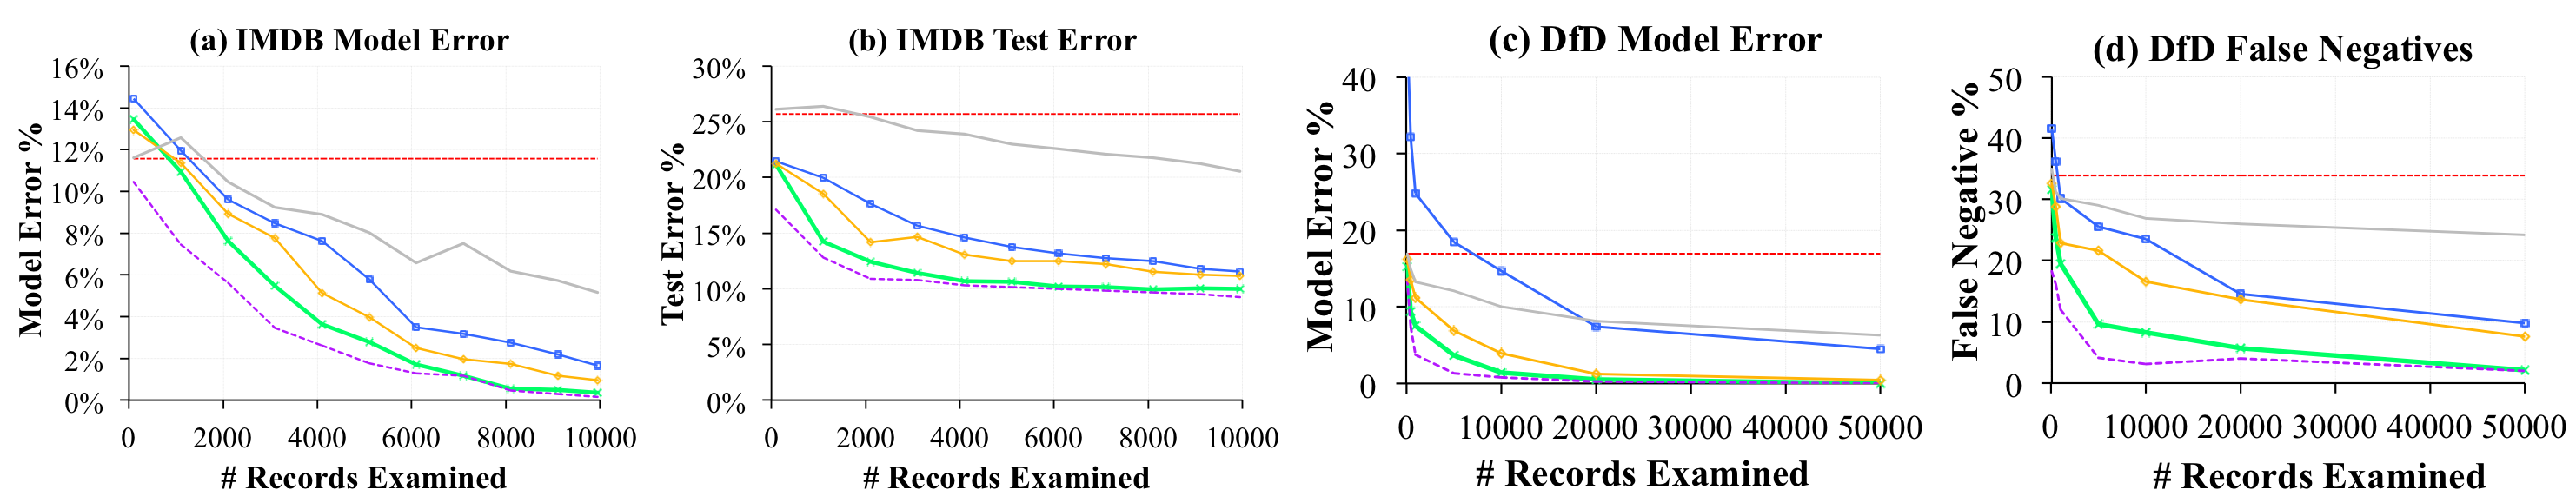
\includegraphics[width=\textwidth]{exp/real-experiments-full.png}
 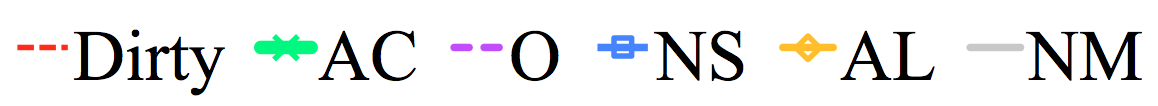
\includegraphics[width=0.6\columnwidth]{exp/legend-real.png}
 \caption{(a) We plot the relative model error as a function of the number of records cleaned for each of the alternatives on the IMDB content tagging task. \sys results in the fastest convergence. (b) Faster convergence translates into improved test accuracy. On a holdout set of 20\%, \sys is more accurate than the alternatives. (c) We evaluate \sys on the Dollars For Docs fraud detection task and find similar results, where \sys converges faster than the alternatives. (d) \sys improves the false negative rate (detection error) of the classifier resulting in an improved fraud detector. \label{real}}
\end{figure*}

\subsection{Real Scenarios}\label{real-errors}
We now describe two data analyst classification scenarios based on popular industry use cases reported in the Apache Spark user survey~\cite{sparksurvey} --- these experiments are run with real data and real corruption.
The first is a content tagging problem to categorize movies from plot descriptions; 
the second is a fraud detection problem to  determine whether a medical donation is suspicious.
Both of the datasets are plagued by systematic errors that affect the classification accuracy by $10-35\%$.
One indication of the systematic nature of the data error is that errors disproportionately affect one class rather than another.
We simulate the analyst's cleaning procedure by looking up the cleaned value in the dataset that we cleaned beforehand.
See~\cite{activecleanarxiv} for constraints, errors, and cleaning methodology, as well as an additional regression scenario.

%\reminder{Can I propose using "Records Examined" as the x-axes instead of "records cleaned"?}

\subsubsection{Movie Prediction}\label{imdb}
The first scenario uses two published datasets about movies, from IMDB~\footnote{\tiny \url{ftp://ftp.fu-berlin.de/pub/misc/movies/database/}} and Yahoo~\footnote{\tiny \url{http://webscope.sandbox.yahoo.com/catalog.php?datatype=r}}.
Each movie has a title, a short 1-2 paragraph plot description, and a list of categories, and the goal is to train a model to predict whether a movie is a ``Horror'' or ``Comedy'' from the description and title.  
The text data was featurized using a TFIDF model.

The IMDB dataset has 486,298 movies and is very dirty.  
The category list of many movies has redundant and possibly conflicting tags (e.g., ``Kids'' and ``Horror'' for the same movie).   
Also, the plot and title text may have errors from the scraping procedure (e.g., ``br\^Cuin, the'').
This dataset also shows experimental evidence for systematic bias.
Horror movies were more likely to be erroneously tagged, and consequently, a classifier trained on the dirty data favored ``Comedy'' predictions.
In contrast, the smaller Yahoo dataset (106,959 movies) is much cleaner, and nearly all of the movies are found in the IMDB dataset.

To clean the category lists, this smaller dataset to cross-referencing records when possible and import categories from Yahoo.
This was done using a simple entity resolution to match movie titles between the two dataset.
When there was a sufficiently close textual match (in terms of title string similarity), we imported the Yahoo dataset's category list to the IMDB dataset.
For the movies that did not match, we appended the records to the IMDB dataset.
Finally, we filtered the dataset for movies whose category lists included ``Horror'' or ``Comedy''.
To clean the parsing errors, we identify common parsing artifacts in each sampled batch and write a script to fix all records with that problem (e.g., remove all instances of ``\^C'').




% The first scenario explores a dataset of movie descriptions scrapped from the Internet Movie Database (IMDB)\footnote{\url{ftp://ftp.fu-berlin.de/pub/misc/movies/database/}}. 
% Each movie has a title, a 1-2 paragraph plot description, and a list of categories.
% We want to train a model that predicts whether a movie is a ``Horror'' movie or a ``Comedy'' from the plot description and the title.
% These textual attributes are featurized using a TFIDF model and stop words are removed. 
% 
% However, since much of this data is user contributed, the category list of the movies is often very dirty with redundant and sometimes conflicting tags (e.g., ``Kids and Family'' and ``Horror''). 
% Furthermore, the dataset was scrapped in HTML and then encoded in Markdown leaving a number of artifacts of parsing in the plot descriptions (e.g., ``results fr\^Celf, the'').
% Fortunately, we were able to find a much smaller but cleaner dataset from Yahoo of 106959 movies, almost all of which were contained in the IMDB dataset.
% Using this cleaner reference dataset, we matched titles and imported categories when possible.
% We also appended the cleaner plot descriptions from Yahoo to the IMDB descriptions when available.
% The clean dataset had about 10\% less examples than the dirty dataset since some movies were marked as neither  ``Horror'' or ``Comedy''.

Figure \ref{real}a plots the model error and test error versus the number of records examined by each algorithm. 
For very small batches of data (e.g., 50 out of 400,000), some of the techniques are actually less accurate than the dirty model. 
This is because the error due to the particular initial sampled batch of dominates, and we find that differences between the techniques are not statistically significant in that regime.
However, as more data is cleaned, we see a clear seperation between the techniques
%as more records are cleaned. 
The purple bottom curve is the Oracle approach, and we find that out of the practical approaches \sys reduces the model error the fastest, and is the only method that converges to the Oracle performance.
Figure~\ref{real}b directly shows how \sys rapidly reduces the test error --- after 2000 records, \sys's test error is within 0.02 of the fully cleaned model.
\sys provides superior convergence for two main reasons.
First, the update algorithm can incorporate both the raw data as well as the smaller set of cleaned records.
This makes \sys less sensitive to sampling error.
Next, \sys also selects records that are more likely to by dirty (Section \ref{det}) and will will most improve the model (Section \ref{dist-samp}).
This is illustrated in \sys's faster convergence curve in the first 2000 cleaned records.

% We find that \sys converges faster than those trained with the alternatives.
% The reasons for this include: (1) \sys samples more data that is likely to be dirty, and (2) \sys selects data that is most valuable to the model.
% This improvement in model convergence translates into large improvements in the accuracy of the model on a holdout set Figure \ref{real}b.
% Figure \ref{real}b illustrates two points: dirty data significantly affects the quality of the model (25\% misclassification rate) and a relatively small amount of data cleaning can greatly improve the quality of the model with the appropriate update techniques.
% For 2000 records cleaned, \sys is within 2\% of the accuracy of the model if the data were fully cleaned.
% On the other hand, for the same amount of cleaning, the ``Re-training'' approach hasn't improved the model. 

% One of the reasons for this positive result is the significant systematic bias in the errors. Horror movies were more likely to be erroneously tagged. 
% On the dirty dataset, the prediction precision of the model for Horror movies was only 29\%.
% This improved to 74\% after data cleaning.

\vspace{1em}
\subsubsection{Dollars For Docs (DfD)}\label{exp:dfd}
The second scenario explores ProPublica's Dollars for Docs dataset described in Section~\ref{s:usecase}.
We featurize the 5 text attributes using a bag-of-words representation, and our goal is to predict the status of medical donations using an SVM (``allowed'' or ``disallowed'').
Figure~\ref{real}c plots the model error as a function of the number of records examined for each of the techniques.
As in the IMDB dataset, we find that \sys converges faster than Naive-Mix, Naive-Sampling, and Active Learning.
In fact, \sys can achieve comparable model accuracy (< 1\% of the true model accuracy) while expending a fraction of the data cleaning effort (10\% of the records cleaned).

In terms of test error, Figure~\ref{real}d reports the detection error or false negative \% (percentage of disallowed research contributions that the model misses) on a held-out evaluation set. 
This measures the real-world utility of the classifier learned with \sys.
The dirty and fully cleaned models have respectively a 34\% and 3\% detection error.
Due to the systematic bias in the data errors (explained in Section \ref{s:usecase}), \sys is able to identify the dirty records and
reduce the detection error to 8\% after examining 10,000 records.

Overall, we found that systematic errors are indeed present in real-world datasets, and that \sys can effectively identify and exploit this bias
to more quickly converge to the true clean model as compared to the naive or active learning approaches.  
In fact, we found that the commonly used retraining approach (Naive-Mix) was almost completely ineffective as compared to other model update techniques.

% The dataset has 240,089 records with 5 textual attributes and one numerical attribute.
% The dataset is featurized with bag-of-words featurization model for the textual attributes which resulted in a 2021 dimensional feature vector, and a binary SVM is used to classify the status of the medical donations.
% Figure \ref{real}c shows that \sys converges faster than Active Learning and SampleClean.
% To achieve a 4\% relative error (i.e., a 75\% error reduction from the dirty model), \sys cleans 40000 fewer records than Active Learning.
% Also, for 10000 records cleaned, \sys has nearly an order of magnitude smaller error than SampleClean.

% Figure \ref{real}d shows the detection rate (fraction of disallowed research contributions identified) of the classifier as a function of the number of records cleaned. 
% On the dirty data, we can only correctly classify 66\% of the suspected examples (88\% overall accuracy due to a class imbalance).
% On the cleaned data, this classifier is nearly perfect with a 97\% true positive rate (98\% overall accuracy).
% \sys converges to the cleaned accuracy faster than the alternatives with a classifier of 92\% true positive rate for only 10000 records cleaned.
% These numbers also indicate the significant systematic bias where positive examples are more likely to be corrupted.

% In short, these two scenarios illustrate the value of \sys on real datasets both of which contain significant systematic biases.
% \sys demonstrates increased accuracy for the same amount of records cleaned compared the alternatives.
% Across all of our experimental datasets, we found that the retraining approach gave poor results in addition to the correctness problems discussed in the introduction.
% For this reason, in future comparisons, we exclude retraining but discuss this in Section \ref{exp:rtr}.

\begin{figure}[t]
\centering
 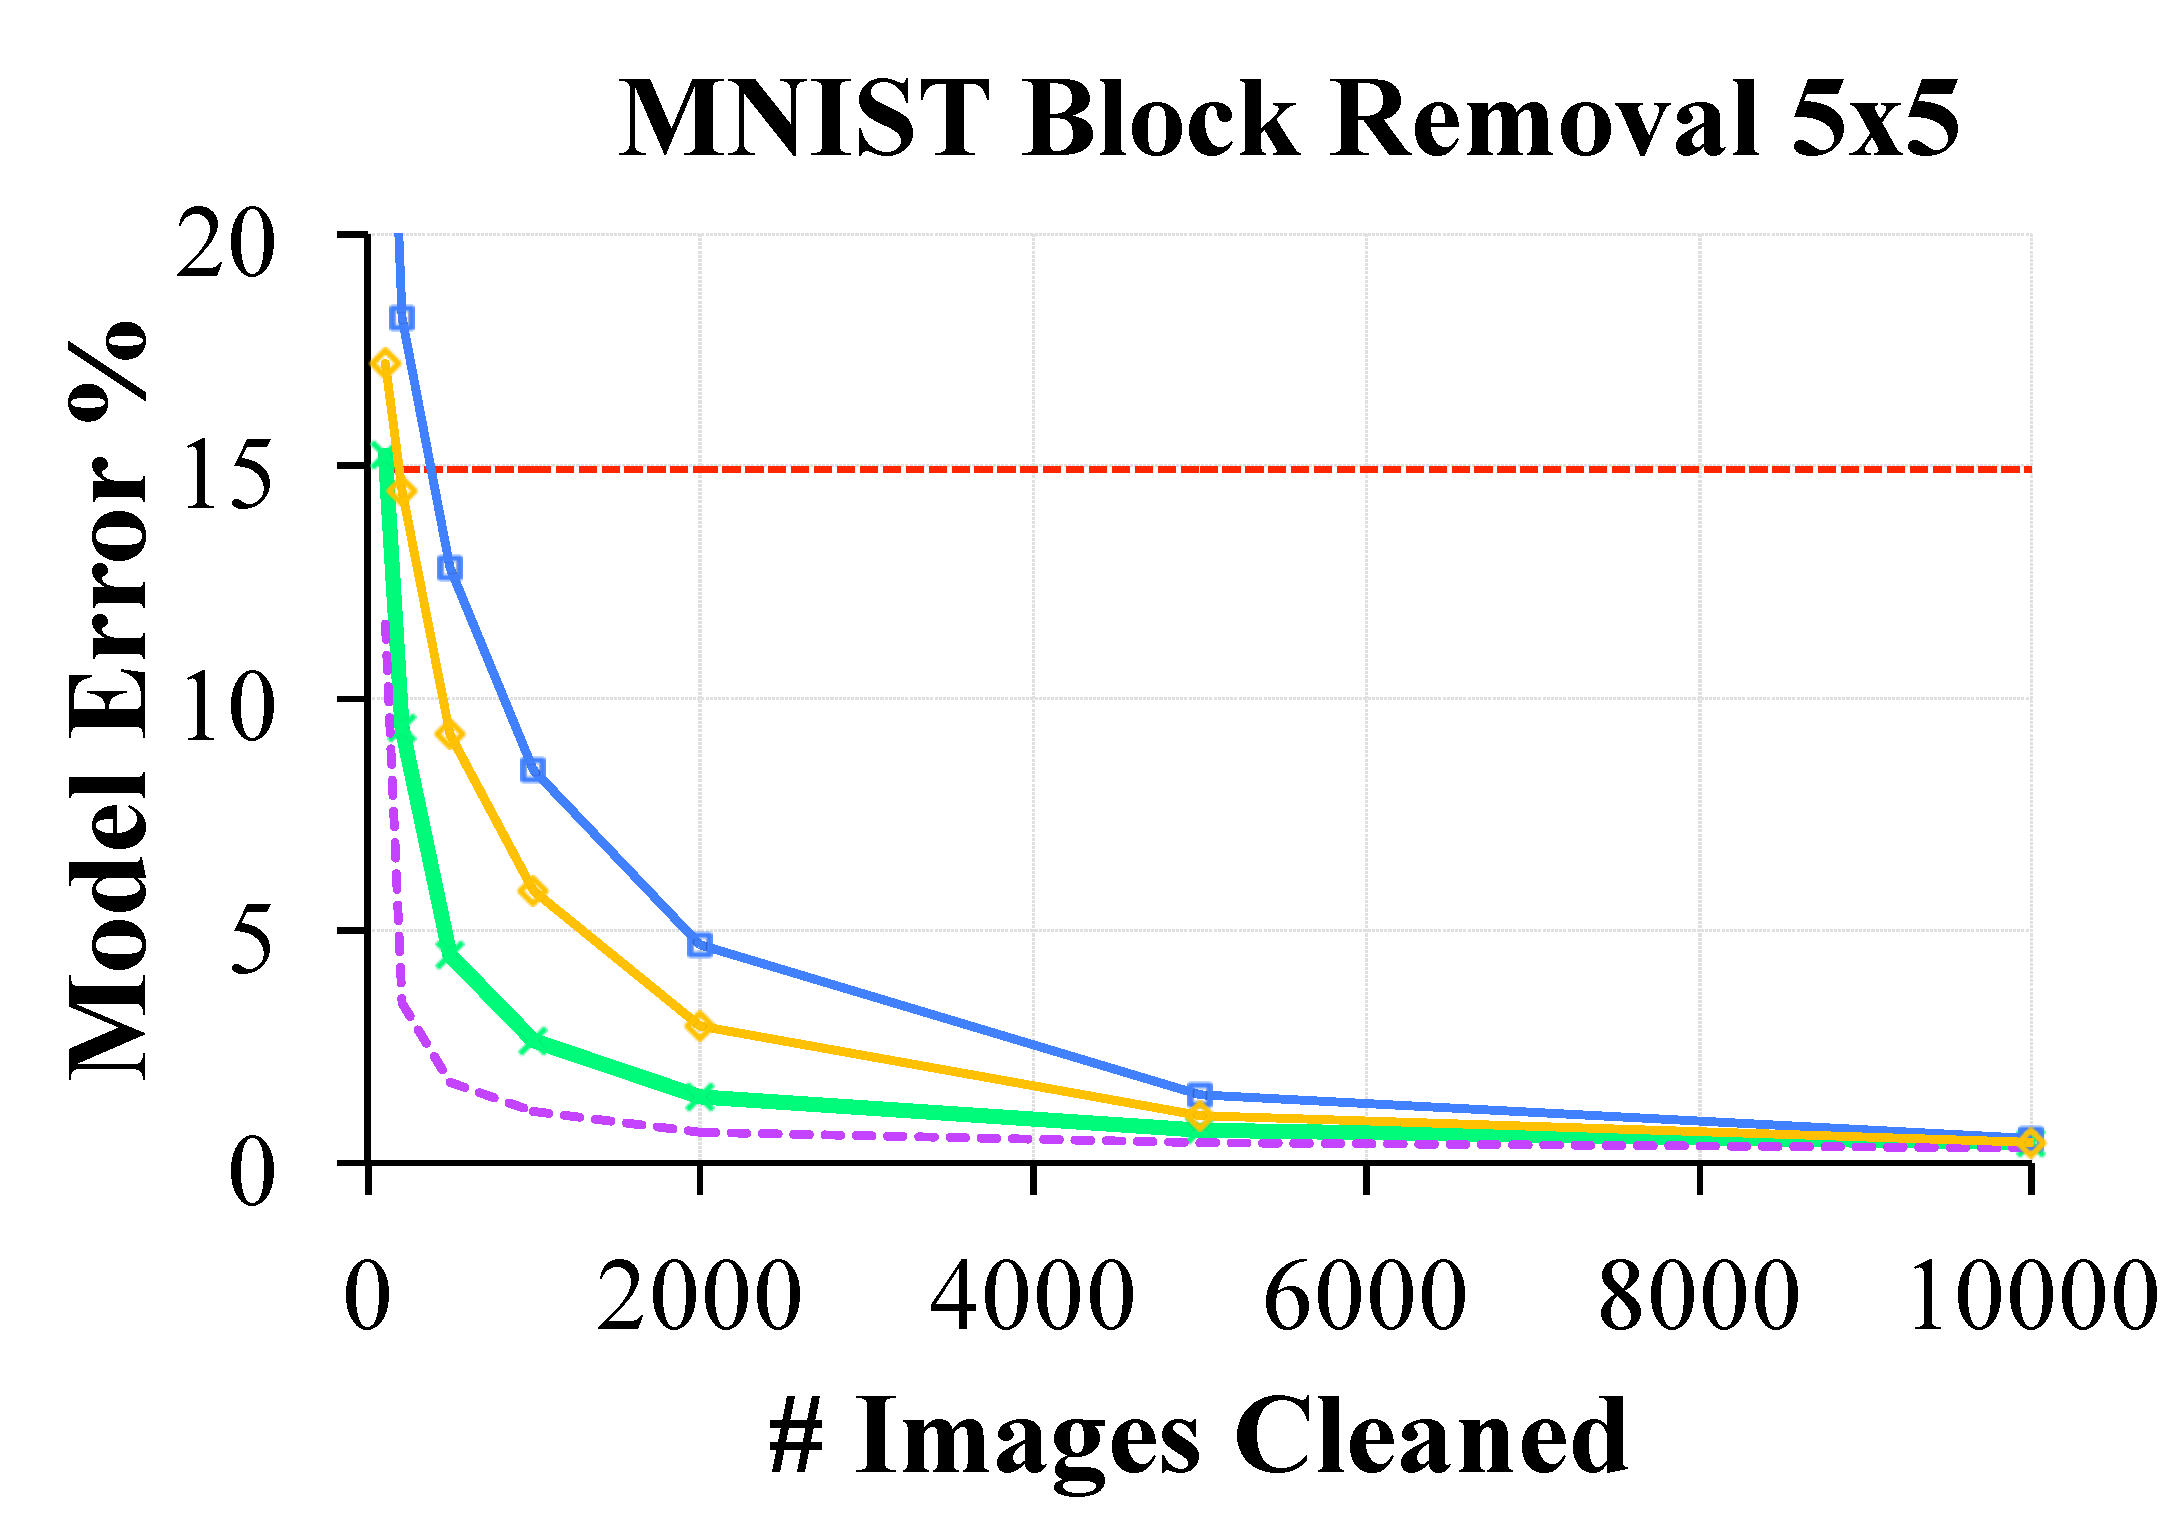
\includegraphics[width=0.49\columnwidth]{exp/exp7a.pdf}
 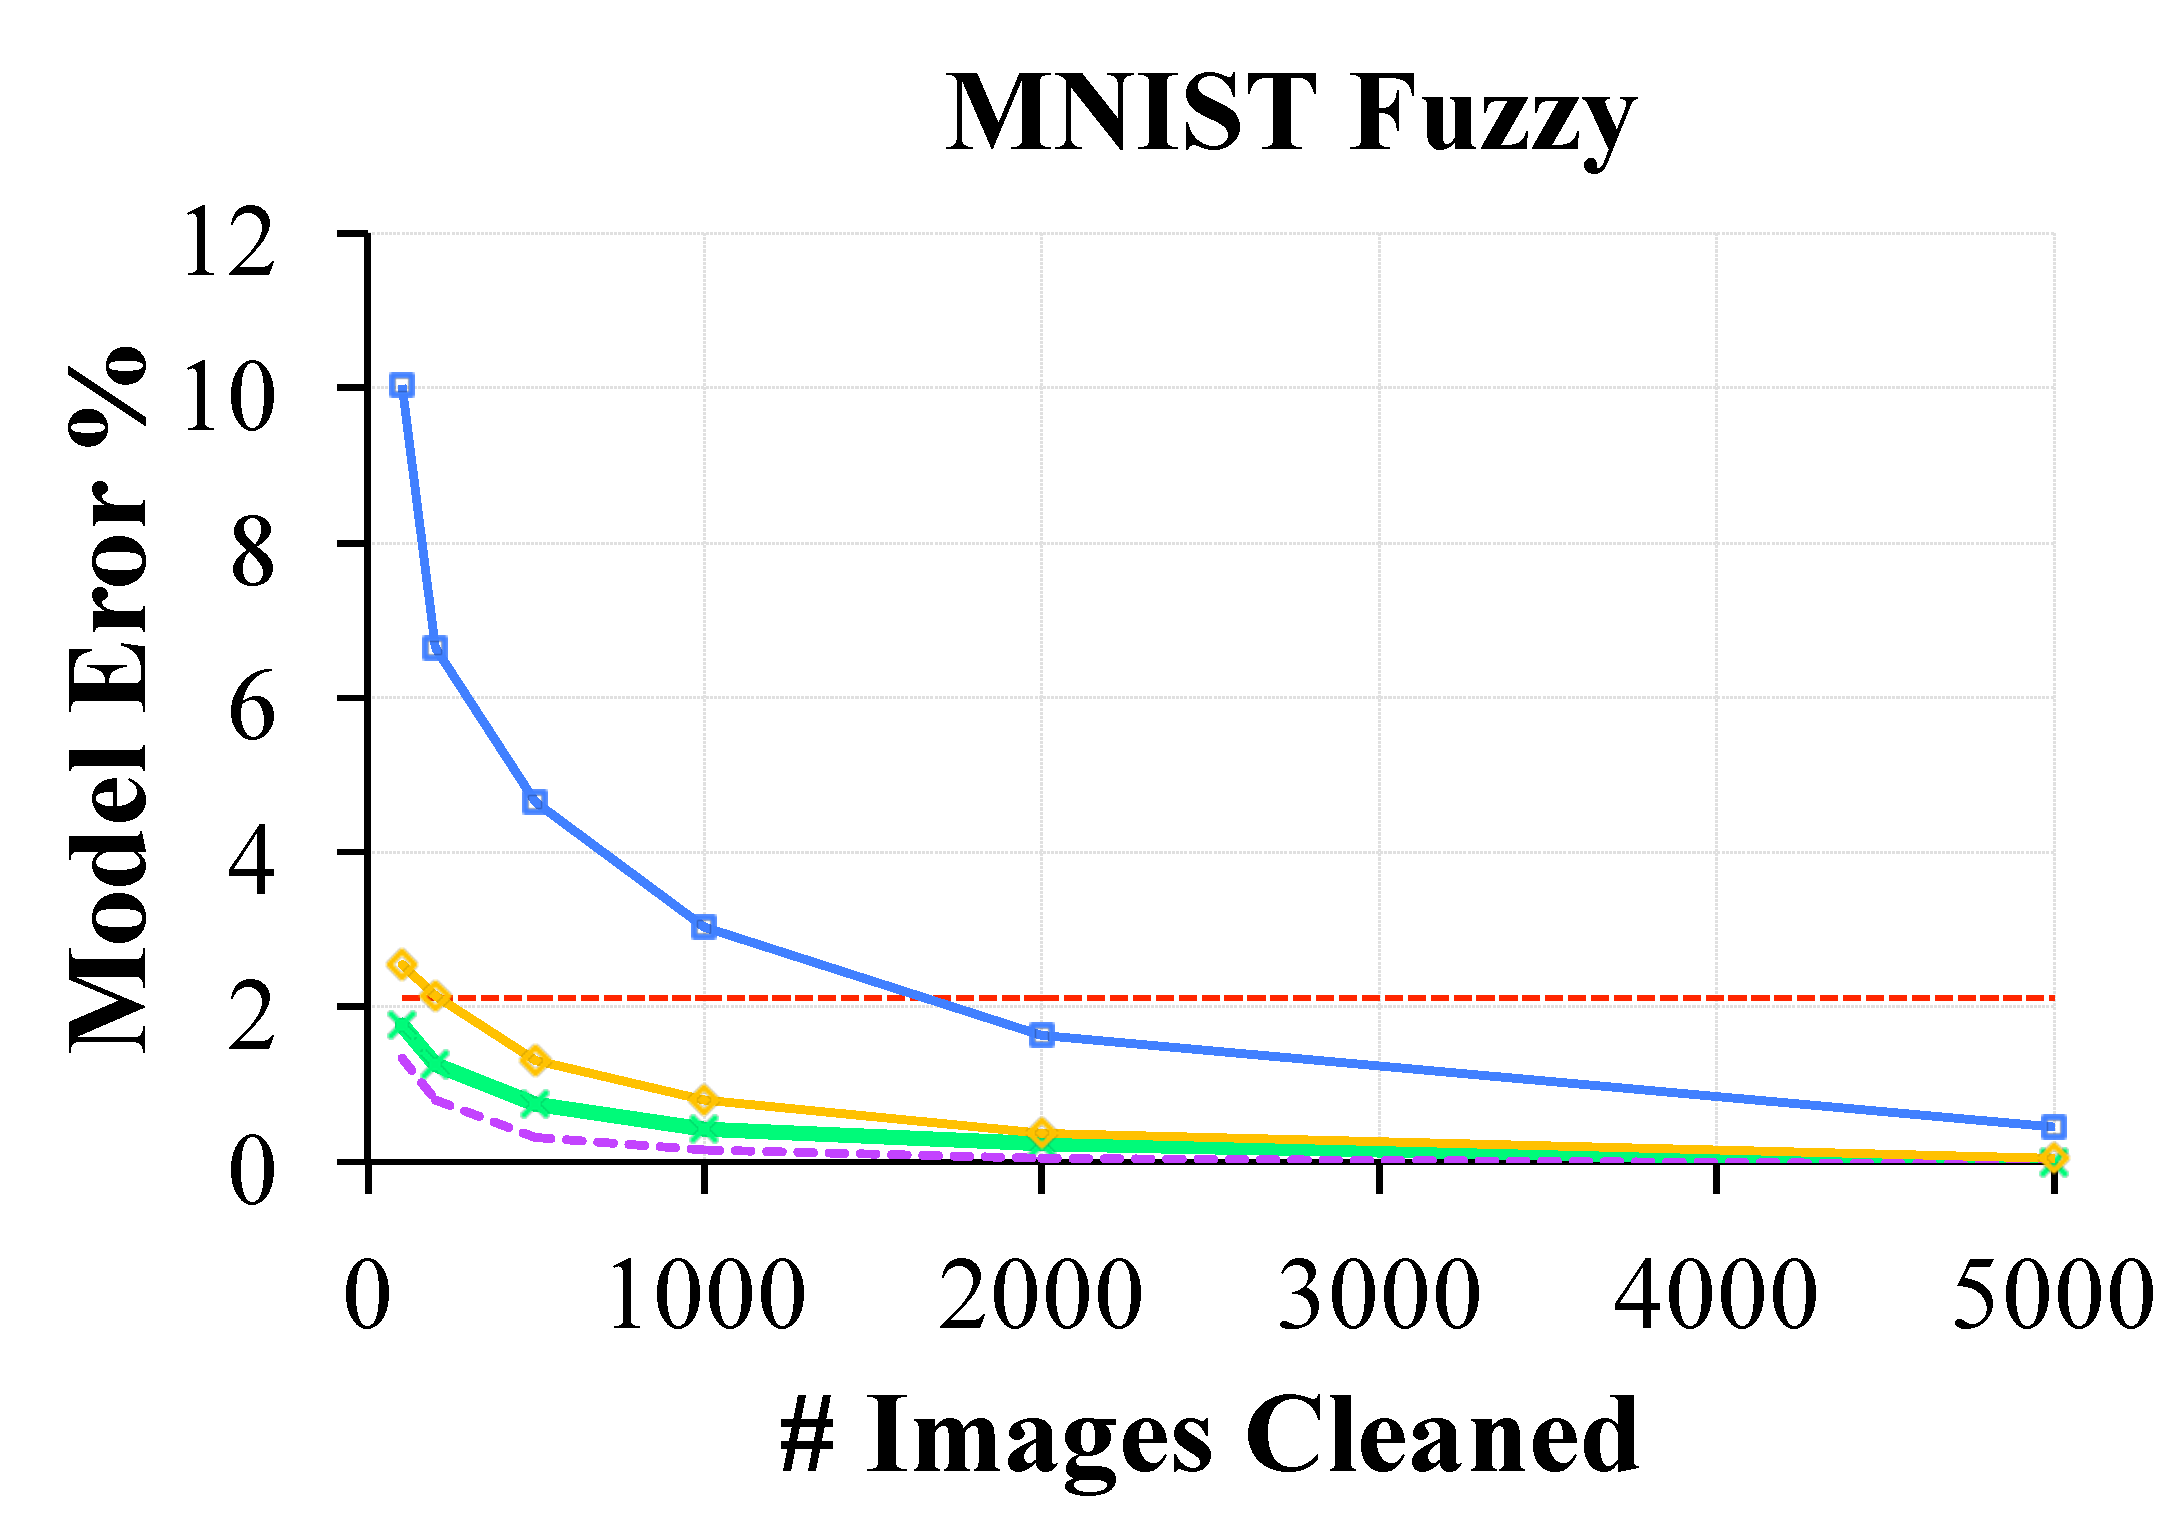
\includegraphics[width=0.49\columnwidth]{exp/exp7b.pdf}
 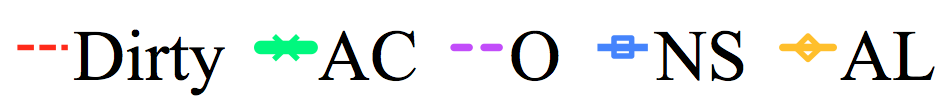
\includegraphics[width=0.49\columnwidth]{exp/legend-general.png}
 \caption{In an image processing pipeline on the MNIST dataset with simulated errors, \sys outperforms Active Learning and Naive-Sample.  \label{mnist}}
\end{figure}

\vspace{4em}
\subsection{Simulated Machine Learning Pipeline}
This experiment is representative of modern machine learning pipelines such as AMPLab's Keystone ML~\cite{keystone} and Google's Tensor Flow~\cite{tensor}. 
The task is to classify 60,000 images of handwritten digits from the MNIST dataset into 10 categories with a one-to-all multiclass SVM classifier~\footnote{\scriptsize\url{http://ufldl.stanford.edu/wiki/index.php/Using_the_MNIST_Dataset}}. 
In contrast to the prior scenarios, which directly extracted feature vectors from the raw dataset, image feature extraction involves a pipeline of transformation steps including edge detection, projection, and raw image patch extraction~\cite{keystone,tensor}.
The cleaning function $C()$ involves replacing a potentially corrupted image with a non-corrupted version.
We find that pipelines tend to propagate small amounts of corruption, and in fact, and even randomly generated errors can morph into systematic biases.
% What is unique about image processing is that data are often processed through a pipeline of operators edge detectors, projections, and raw image patches~\cite{keystone,tensor}.
% This experiment explores data cleaning in this context, where dirtiness is in the raw data but get propagated through the pipeline.

% We use the MNIST handwritten digit recognition dataset with a MATLAB image processing pipeline.
% In this scenario, the analyst must inspect a potentially corrupted image and replace it with a higher quality one.
% The MNIST dataset consists of 64x64 grayscale images.
There are two types of simulated corruptions that mimic standard corruptions in image processing (occlusion and low-resolution): \texttt{5x5 Removal} deletes a random 5x5 pixel block by setting the pixel values to 0, and \texttt{Fuzzy} blurs the entire image using a 4x4 moving average patch. 
We apply these corruptions to a random 5\% of the images.

Figure \ref{mnist} shows that \sys makes more progress towards the clean model with a smaller number of examples cleaned.
To achieve a 2\% error for 5x5 Removal, \sys can inspect 2200 fewer images than Active Learning and 2750 fewer images than Naive-Sampling.
For the fuzzy images, both Active Learning and \sys reach 2\% error after examining $<100$ images, while Naive-Sampling requires 1750.
Even though these corruptions are generated independently of the data, the \texttt{5x5 Removal} propagates through the pipeline as a systematic error.
The image features are constructed with edge detectors, which are highly sensitive to this type of corruption.
Digits that naturally have fewer edges than others are disproportionately affected since the removal process adds spurious edges.
On the other hand, the \texttt{Fuzzy} corruption propagates through the pipeline are similar to random errors (as opposed to systematic).
%This experiment highlights that featurization and other data processing pipelines between the raw data and model can introduce systematic biases in the presence of data corruption.

\subsection{Simulated Error Scenarios}
In the next set of experiments, we use standard Machine Learning benchmark datasets and corrupt them with varying levels of systematic noise.
We use this to evaluate \sys while isolating certain variables.
The two datasets that we used were:

\vspace{0.25em}

\noindent\textbf{Income Classification (Adult): } In this dataset of 45,552 records, the task is to predict the income bracket (binary) from 12 numerical and categorical covariates with an SVM classifier. 

\vspace{0.25em}

\noindent\textbf{Seizure Classification (EEG): } In this dataset, the task is to predict the onset of a seizure (binary) from 15 numerical covariates with a thresholded Linear Regression. There are 14980 data points in this dataset. This classification task is inherently hard with an accuracy on the completely clean data of only 65\%.

\begin{figure}[t]
\centering
 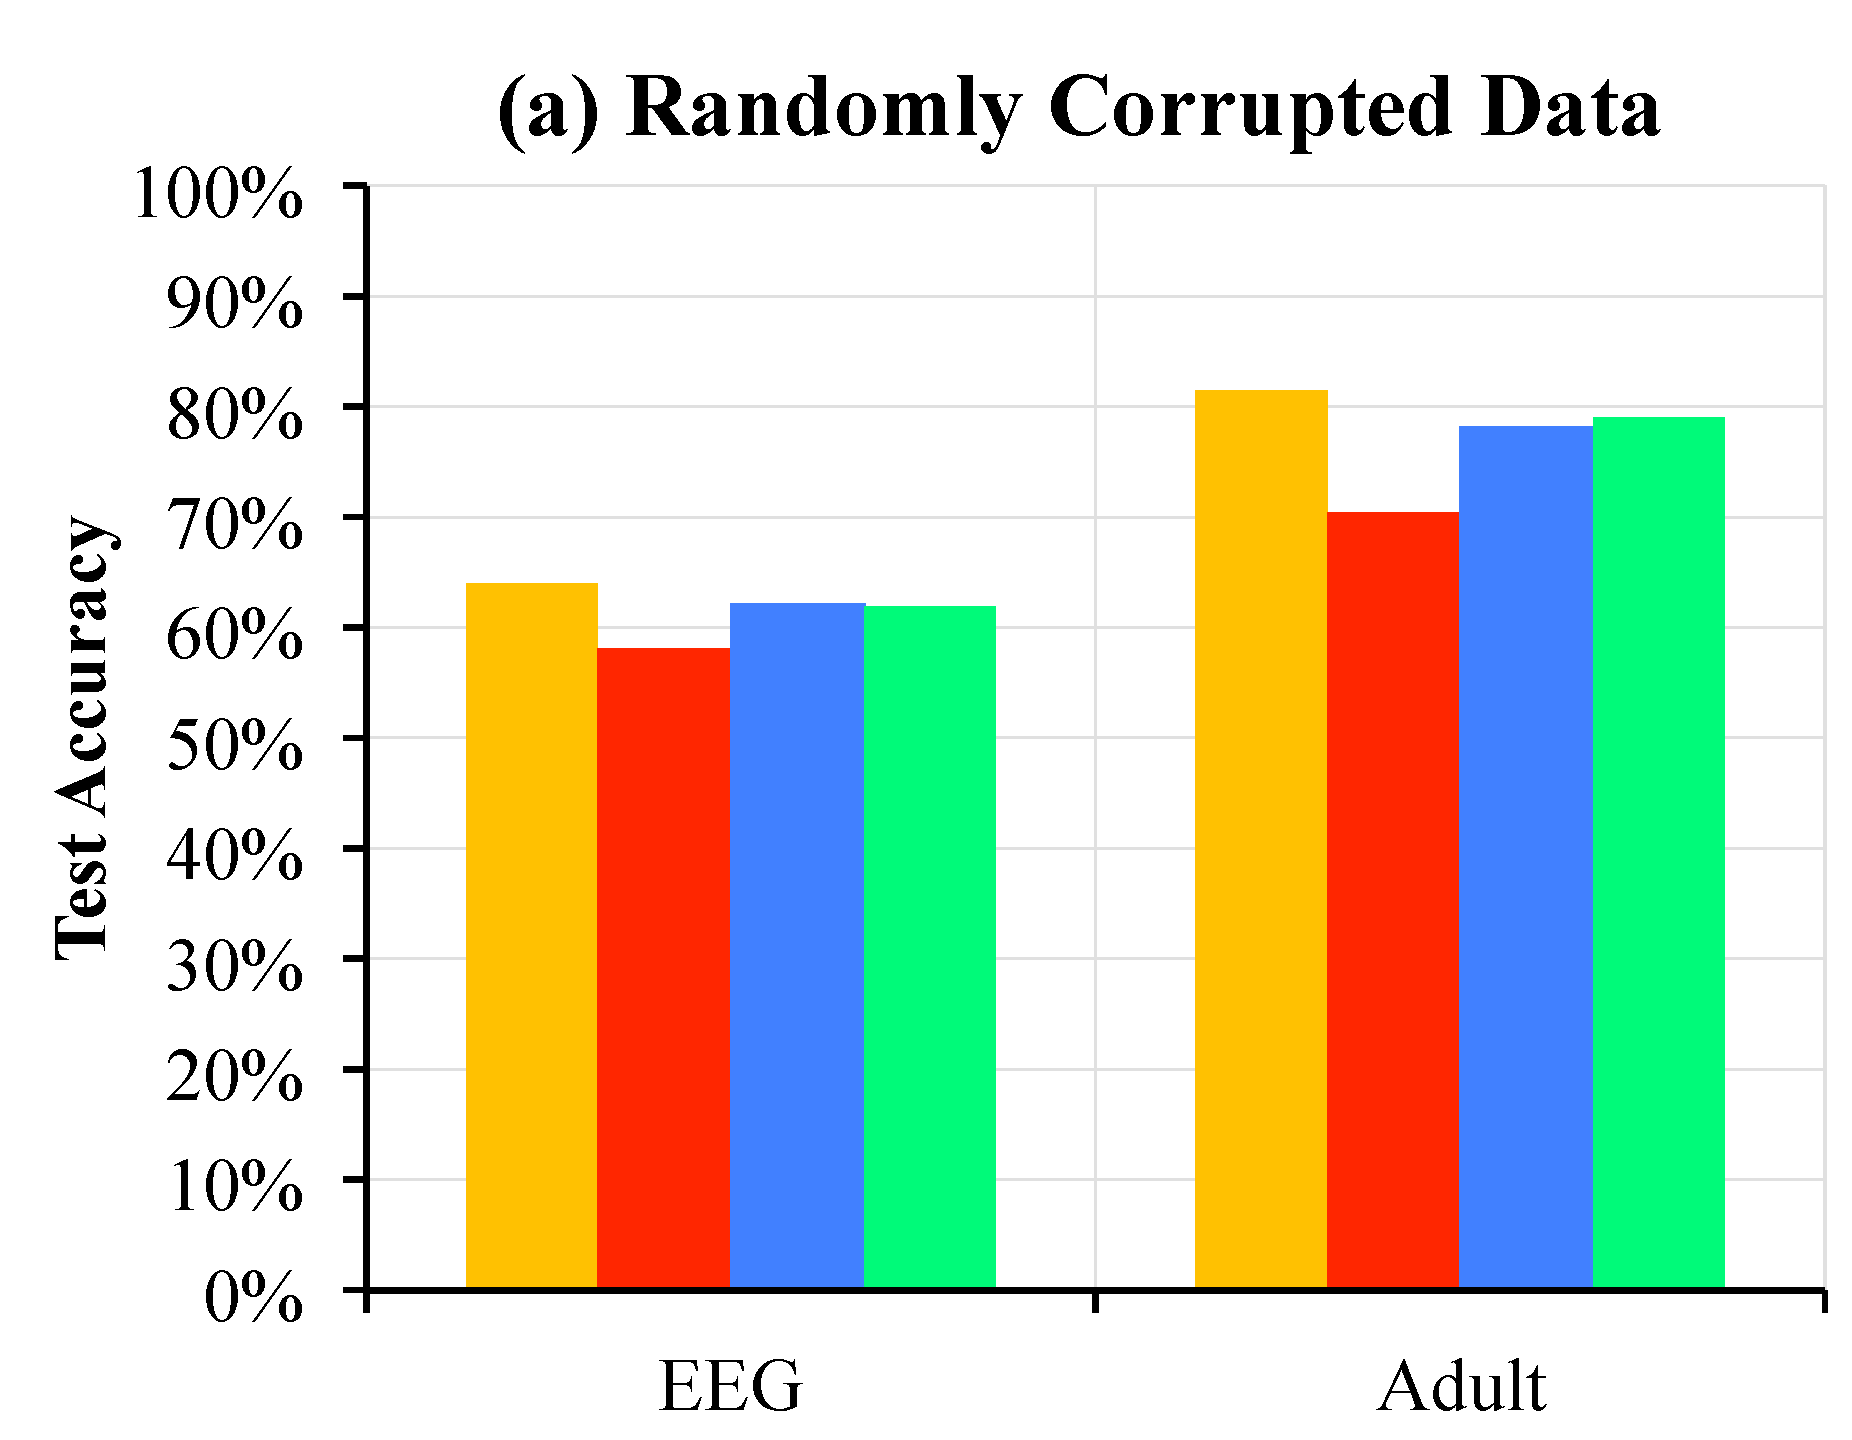
\includegraphics[width=0.49\columnwidth]{exp/exp2.pdf}
 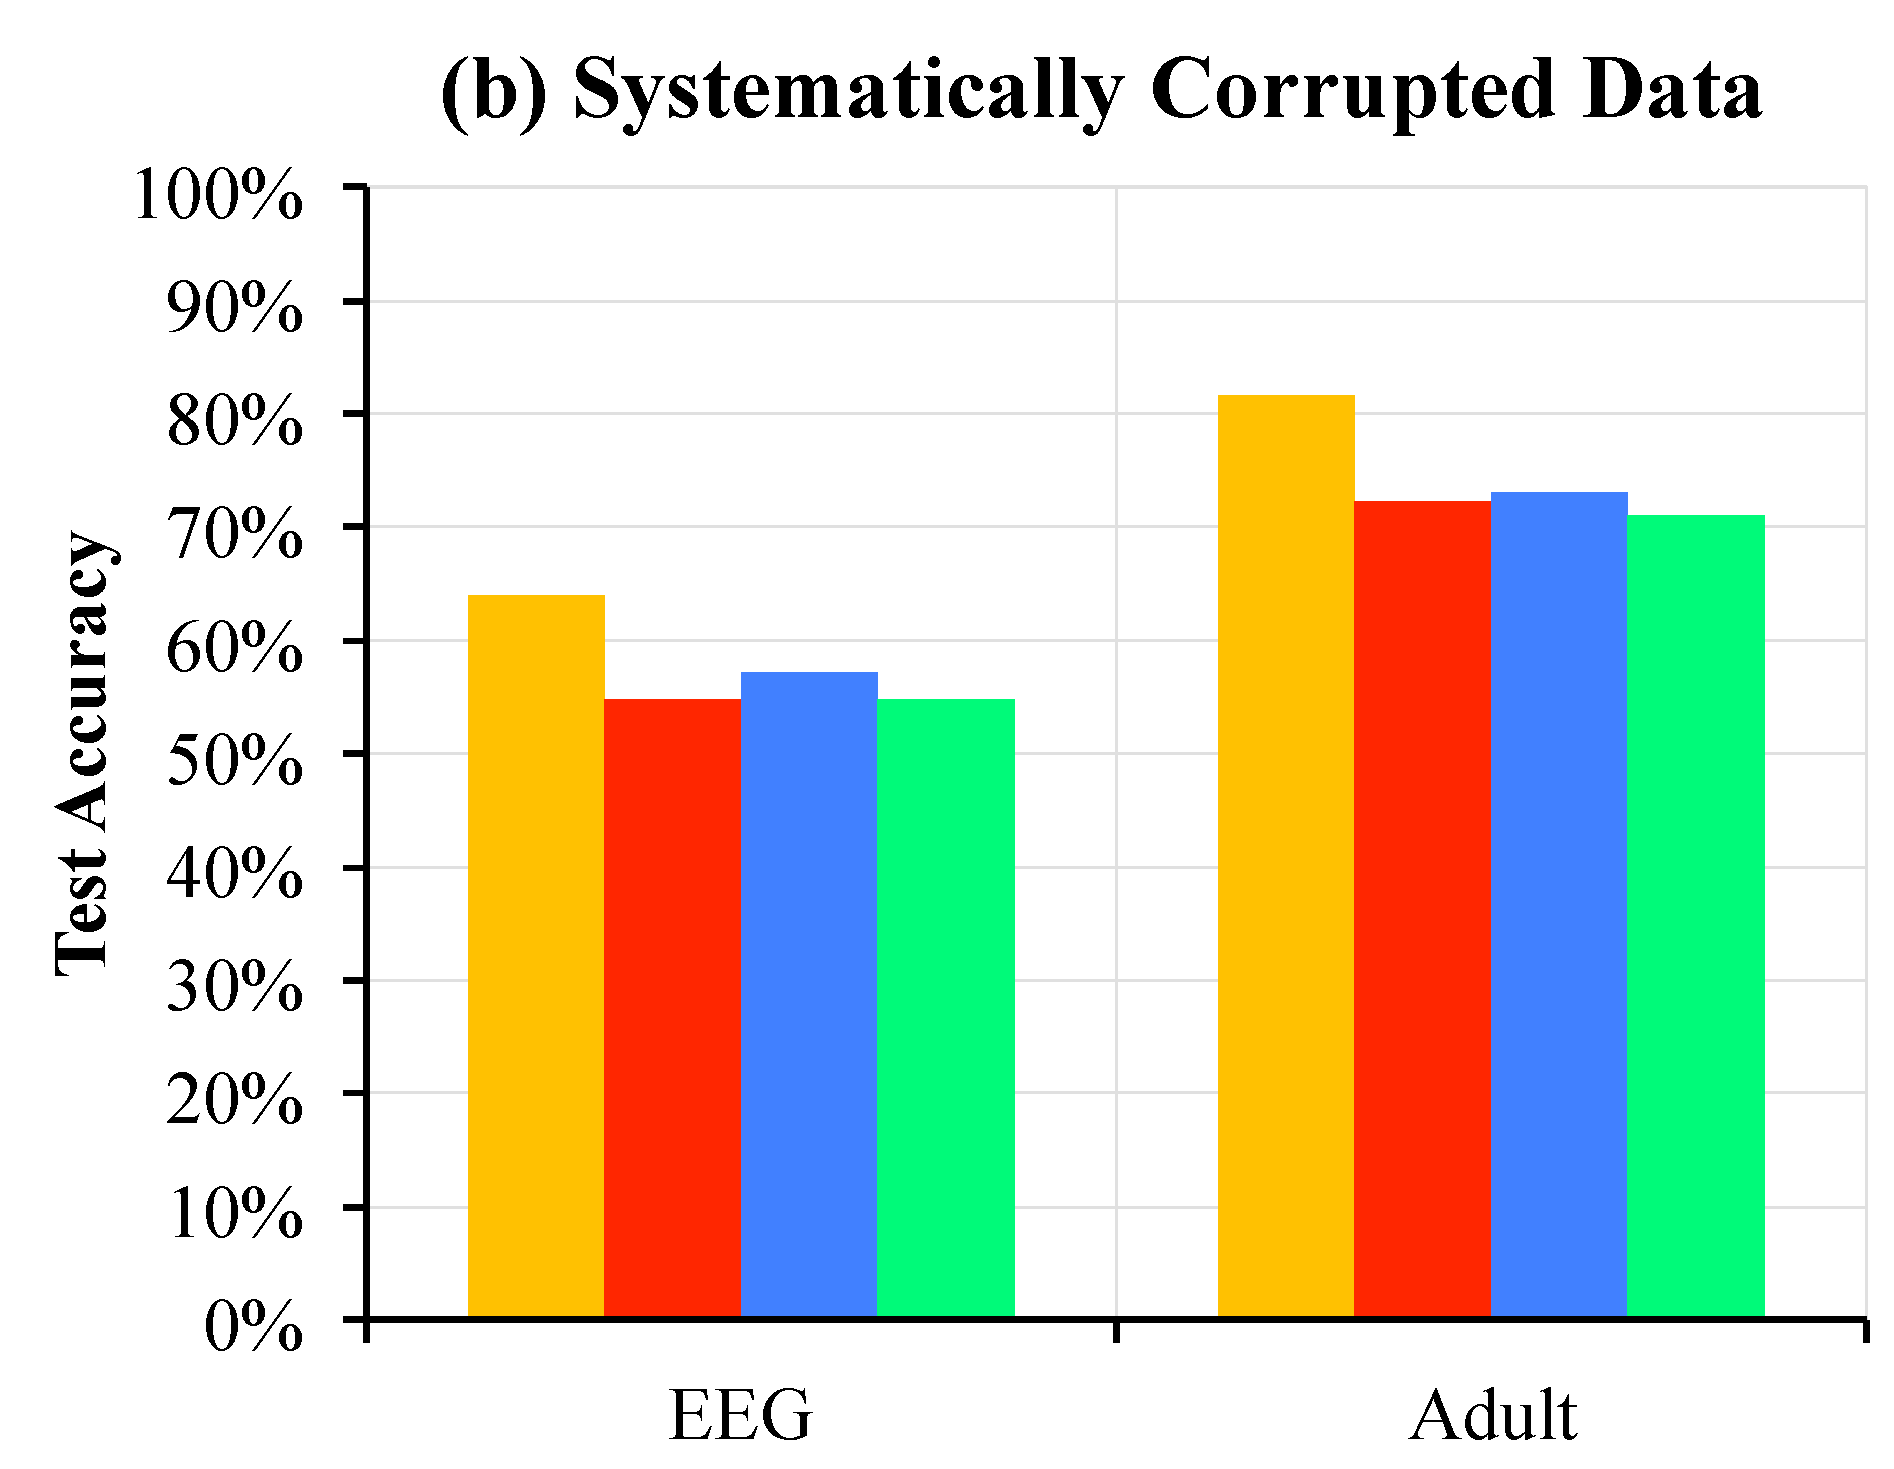
\includegraphics[width=0.49\columnwidth]{exp/exp1.pdf}
 
\includegraphics[width=0.5\columnwidth]{exp/legend-1.png}
 \caption{(a) Robust techniques and discarding data work when corrupted data are random and look atypical. (b) Data cleaning can provide reliable performance in both the systematically corrupted setting and randomly corrupted setting.\label{sys-rand}}
\end{figure}

\subsubsection{Data Cleaning v.s. Robust Statistics}
Machine Learning has broadly studied a number of \emph{robust} methods to deal with some types of outliers. In particular, this field studies random high-magnitude outliers and techniques to make statistical model training agnostic to their presence. Feng et al. proposed a variant of logistic regression that is robust to outliers~\cite{feng2014robust}. We chose this algorithm because it is a robust extension of the convex regularized loss model, leading to a better apples-to-apples comparison between the techniques.
Our goal is to understand which types of data corruption are amenable to data cleaning and which are better suited for robust statistical techniques.
The experiment compares four schemes: (1) full data cleaning, (2) baseline of no cleaning, (3) discarding the dirty data, and (4) robust logistic regression. 
We corrupted 5\% of the training examples in each dataset in two different ways:

\vspace{1em}

\noindent\textbf{Random Corruption: } Simulated high-magnitude random outliers. 5\% of the examples are selected at random and a random feature is replaced with 3 times the highest feature value.

\vspace{0.5em}

\noindent\textbf{Systematic Corruption: } Simulated innocuous looking (but still incorrect) systematic corruption. The model is trained on the clean data, and the three most important features (highest weighted) are identified. The examples are sorted by each of these features and the top examples are corrupted with the mean value for that feature (5\% corruption in all). 
%It is important to note that examples can have multiple corrupted features.

\vspace{1em}

Figure \ref{sys-rand} shows the test accuracy for models trained on both types of data with the different techniques.
The robust method performs well on the random high-magnitude outliers with only a 2.0\% reduction in clean test accuracy for EEG and 2.5\% reduction for Adult.
In the random setting, discarding dirty data also performs relatively well.
However, the robust method falters on the systematic corruption with a 9.1\% reduction in clean test accuracy for EEG and 10.5\% reduction for Adult.
Data cleaning is the most reliable option across datasets and corruption types.
The problem is that without cleaning, there is no way to know if the corruption is random or systematic and when to trust a robust method.
While data cleaning requires more effort, it provides benefits in both settings.
The remaining experiments, unless otherwise noted, use systematic corruption.

\subsubsection{Source of Improvements}\label{comp}
This experiment compares the performance of \sys with and without various optimizations for 500 records examined. 
\sys without detection is denoted as (AC-D) (that is at each iteration we sample from the entire dirty data), and \sys without detection and our prioritized sampling is denoted as (AC-D-I).
Figure \ref{opts} plots the relative error of the alternatives and \sys with and without the optimizations.
Without detection (AC-D), \sys is still more accurate than Active Learning.
Removing the sampling, \sys is slightly worse than Active Learning on the Adult dataset but is comparable on the EEG dataset.
The advantage of \sys is that it is a composable framework supporting different instantiations of the detection and prioritization modules while still preserving convergence guarantees.
With these optimizations, \sys is consistently more efficient than Active Learning.

\begin{figure}[t]
\centering
 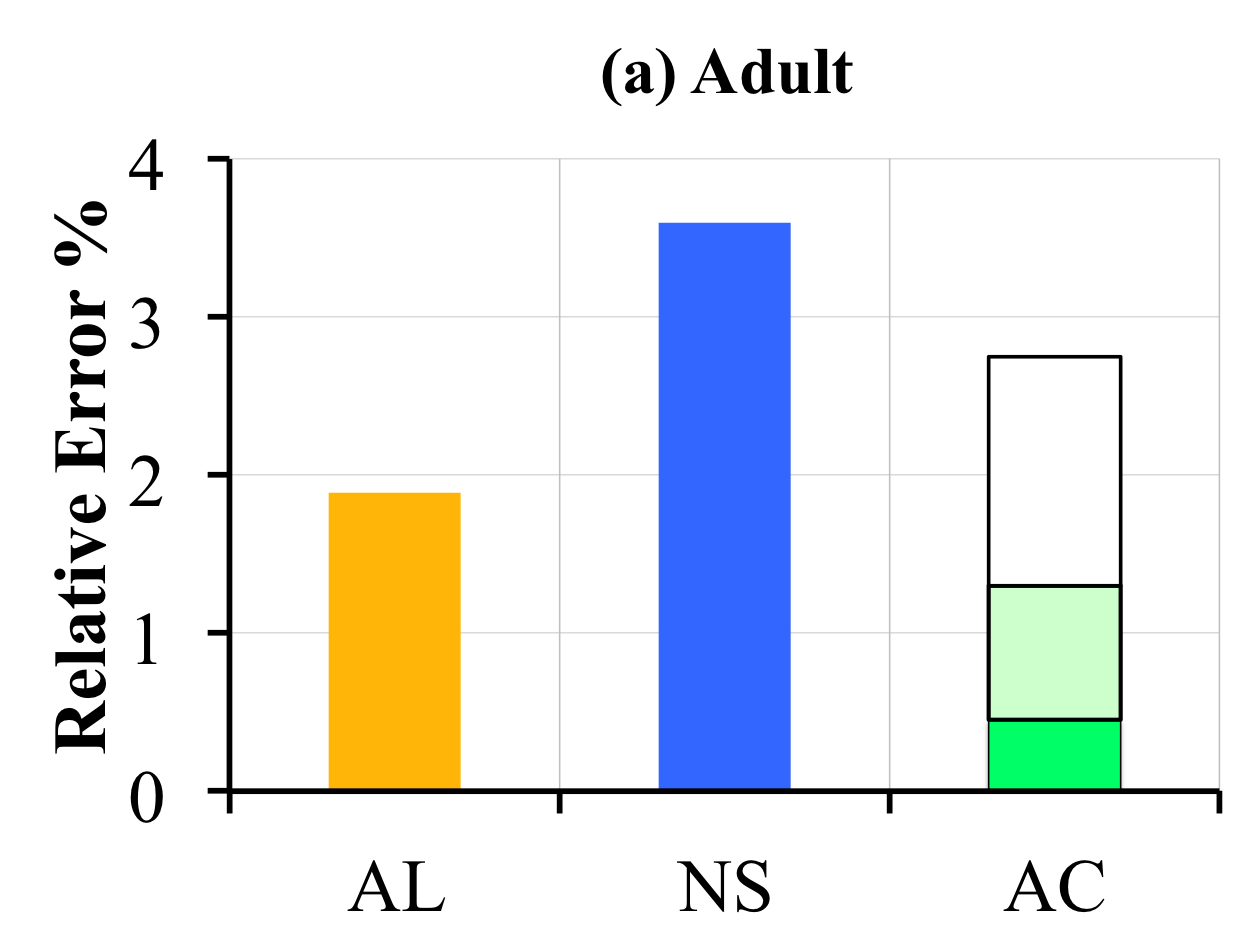
\includegraphics[width=0.49\columnwidth]{exp/exp8a.png}
 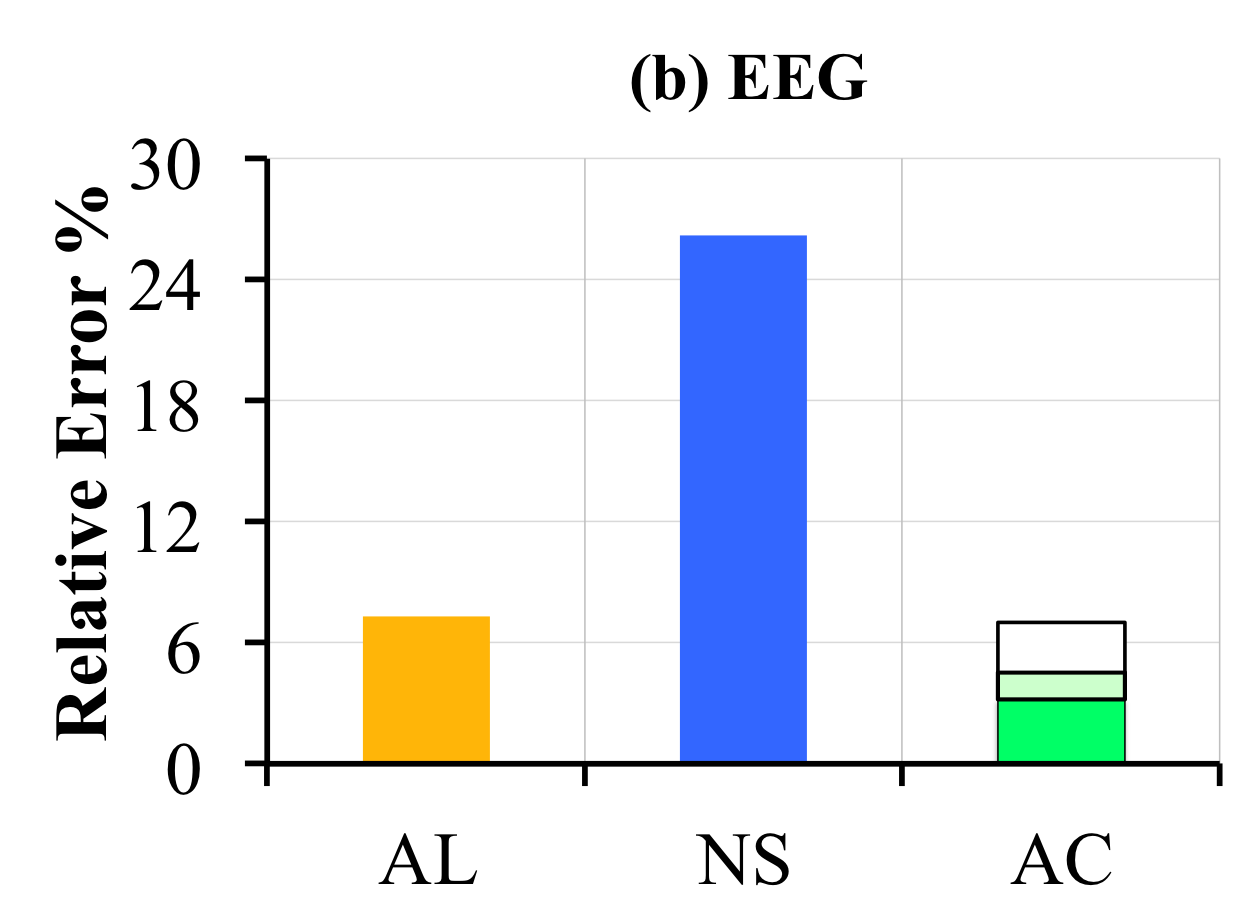
\includegraphics[width=0.49\columnwidth]{exp/exp8b.png}
 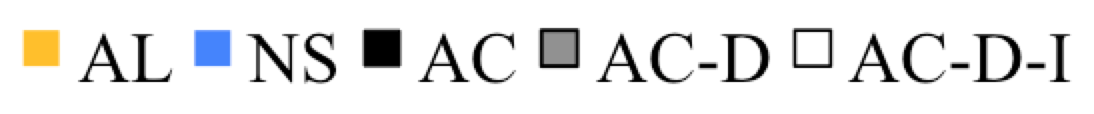
\includegraphics[width=0.5\columnwidth]{exp/legend-8.png}
 \caption{ -D denotes no detection, and -D-I denotes no detection and no importance sampling. Both optimizations significantly help \sys outperform Naive-Sampling and Active Learning. \label{opts}}
\end{figure}

\subsubsection{Mixing Dirty and Clean Data}\label{exp:rtr}
Naive-Mix is an unreliable methodology lacking the same guarantees as Active Learning or Naive-Sampling even in the simplest of cases.
We also saw that it is significantly less efficient than \sys, Naive-Sampling, and Active Learning on the real datasets.
For thoroughness, these experiments include the model error as a function of records examined in comparison to \sys.
We also evaluate this approach with our detection component.
Naive-Mix+D randomly samples data using the dirty data detector, applies the user-specified cleaning, and writes-back the cleaned data.

Figure \ref{pc-perf} plots the same curves as the previous experiment comparing \sys, Active Learning, and two mixed data algorithms.
Intuitively, Naive-Mix makes less progress with each update.
Consider the case where 10\% of the dataset is corrupted and a small sample of data 1\%.
\sys and Naive-Sampling extrapolate from the cleaned sample (\sys extrapolates a gradient) while Naive-Mix considers the entire dirty data which might be much larger.

%\sys converges faster.
%\sys tunes the weighting when averaging dirty and clean data into the gradient.

\begin{figure}[ht!]
\centering
 %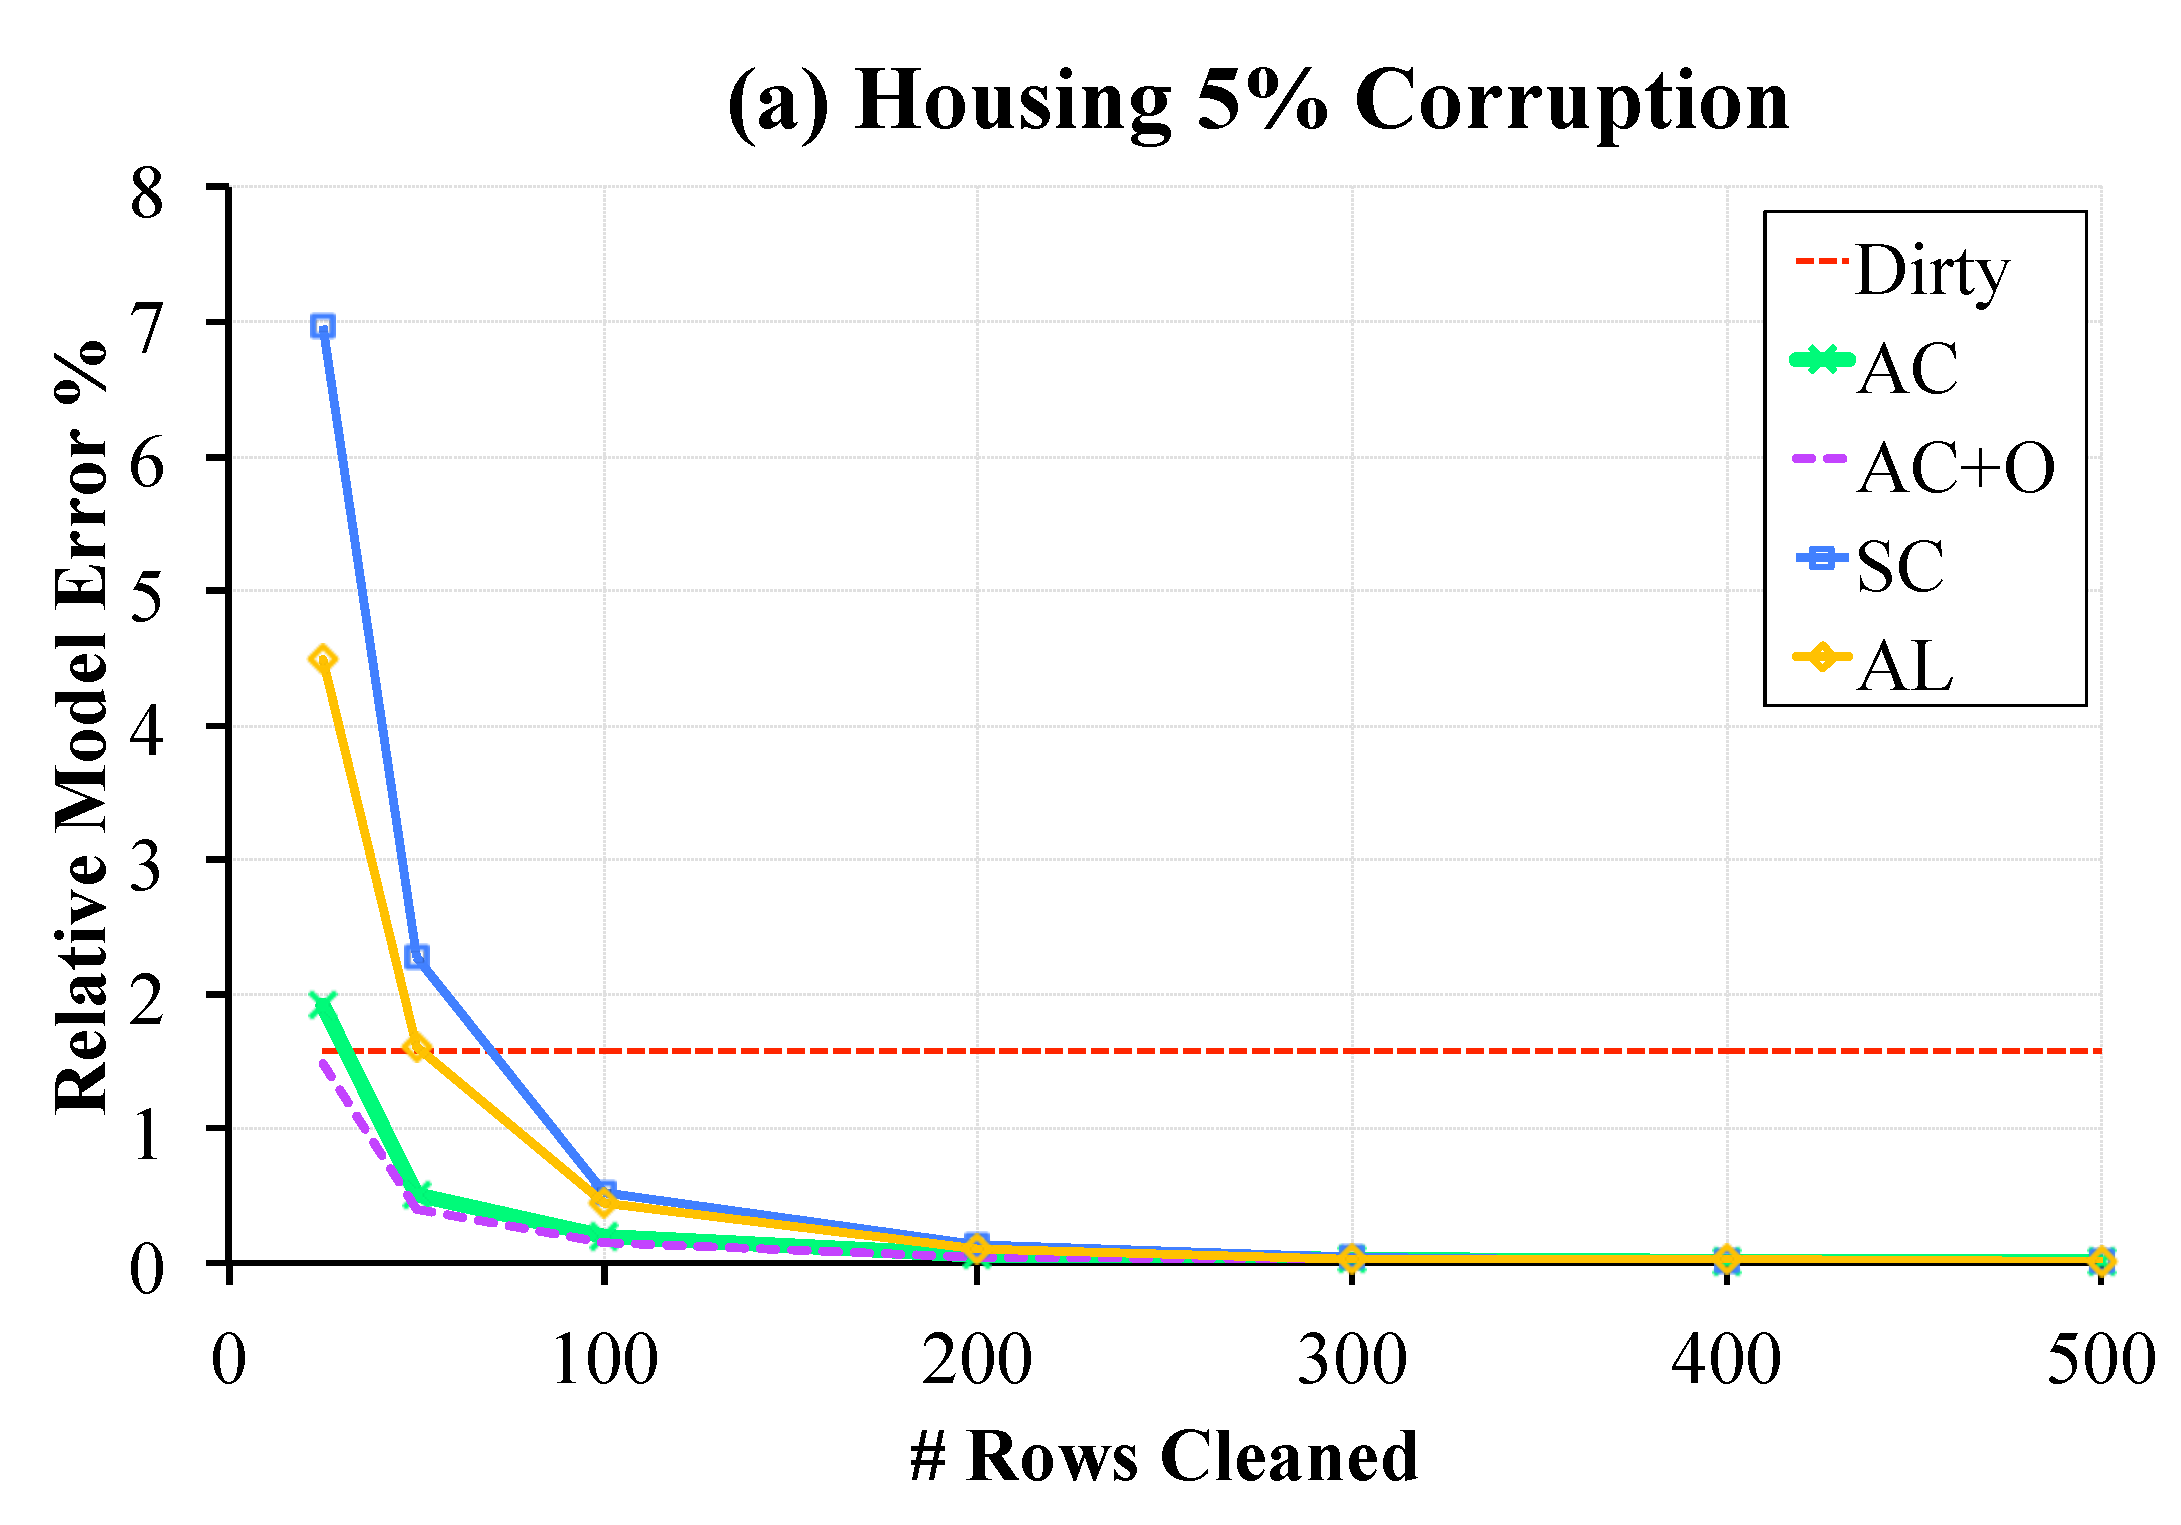
\includegraphics[scale=0.15]{exp/exp3a.pdf}
 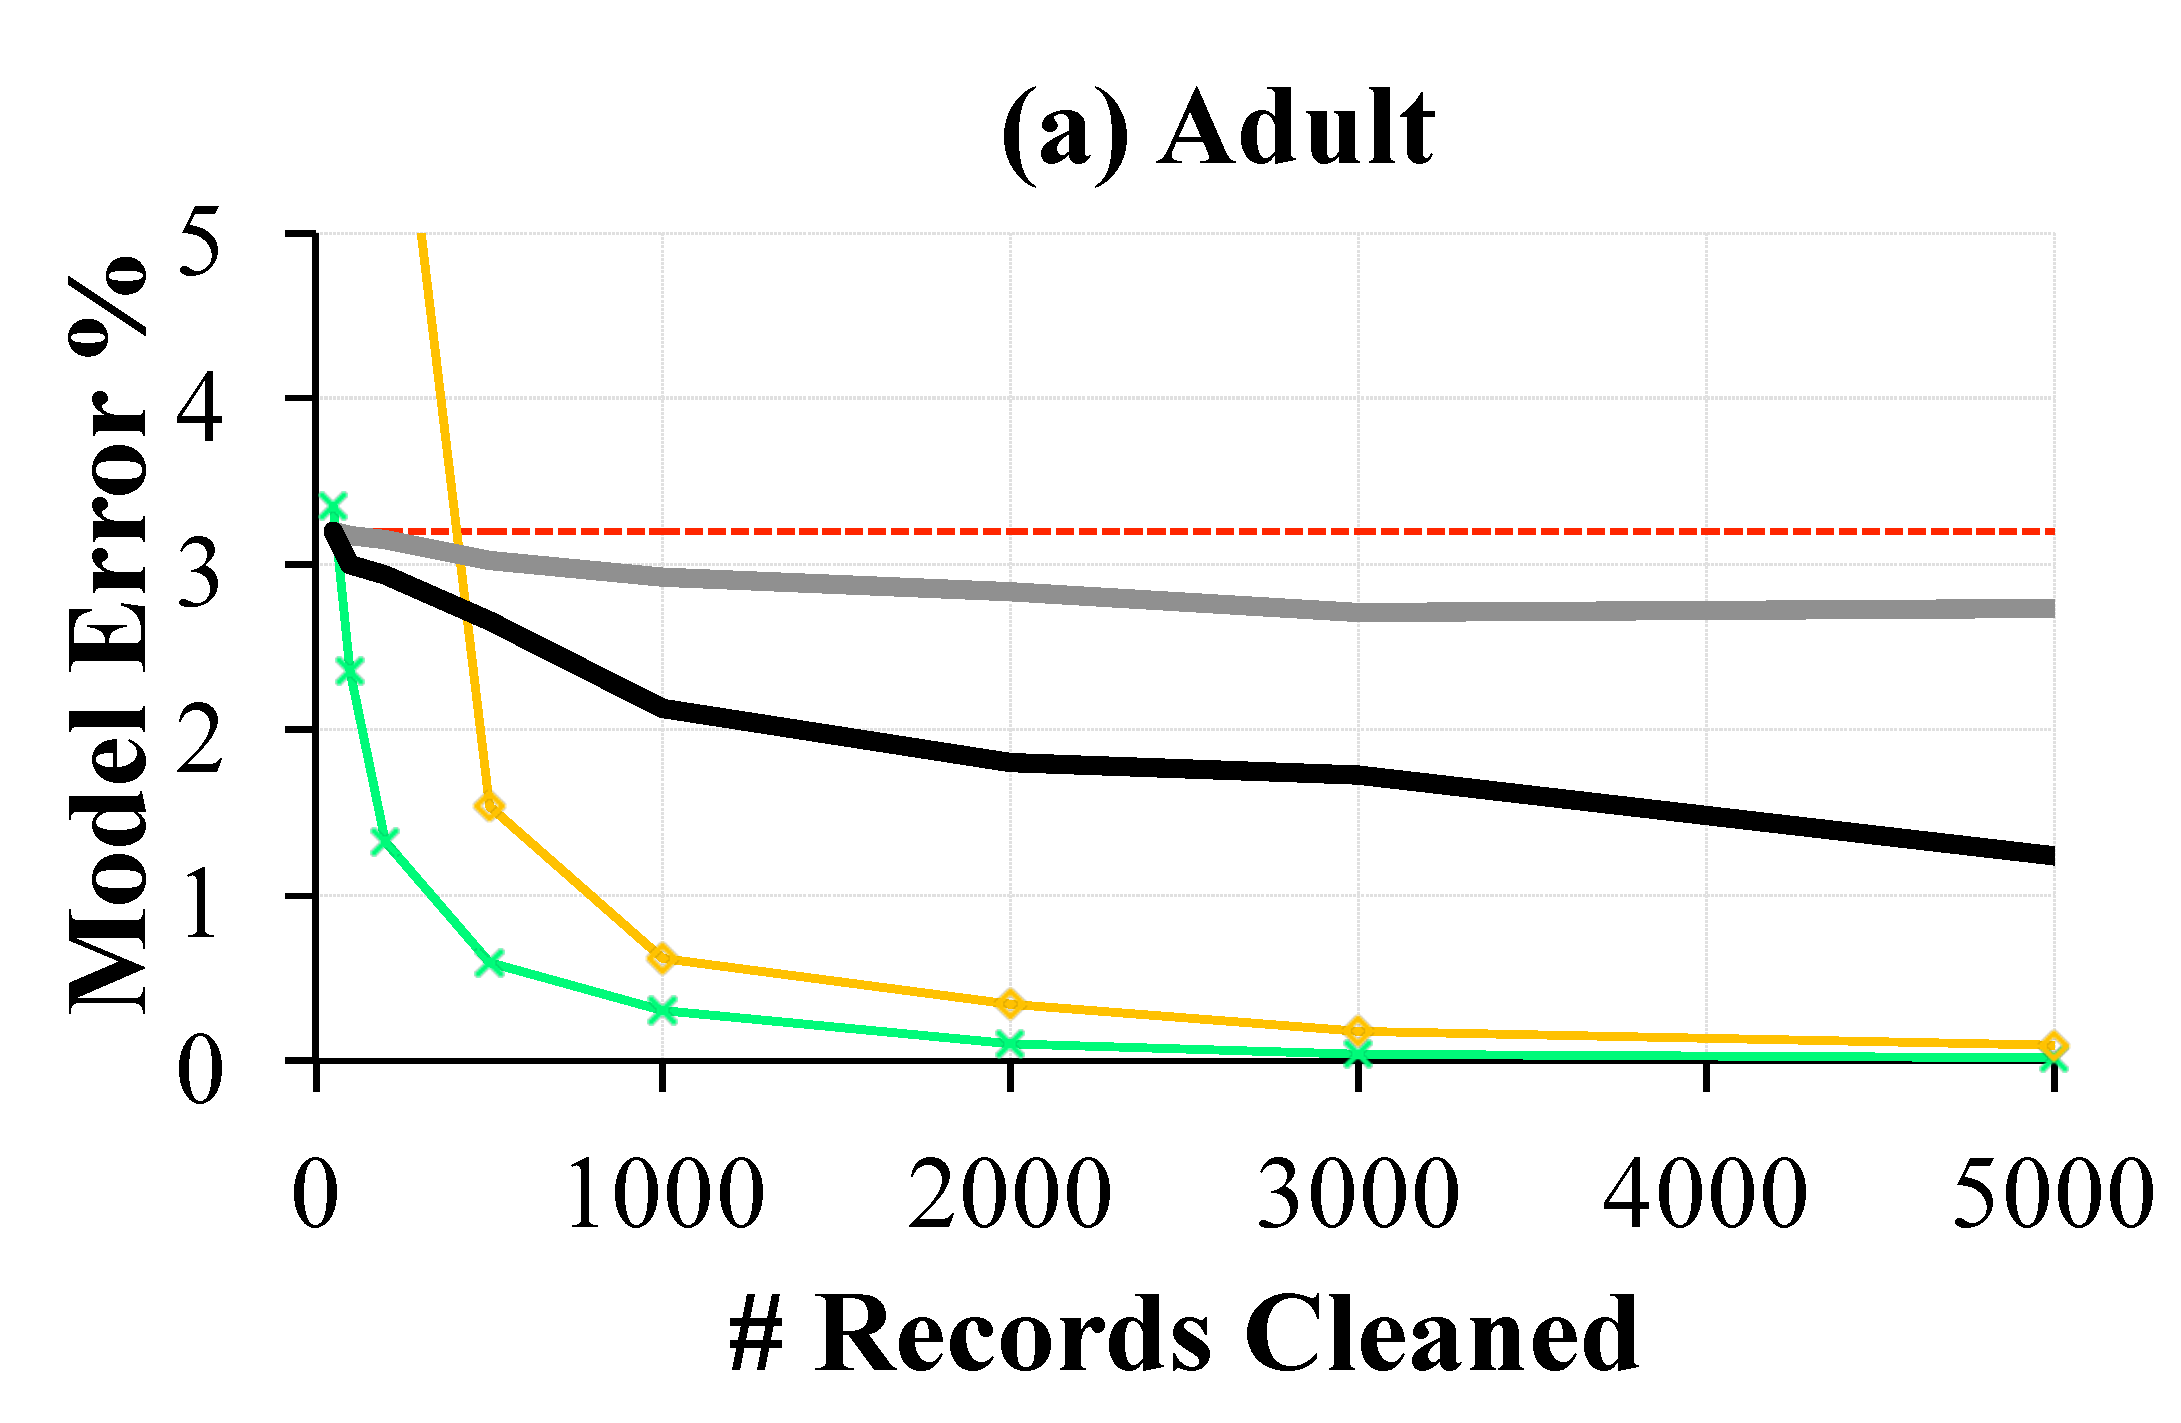
\includegraphics[width=0.49\columnwidth]{exp/exp14a.pdf}
    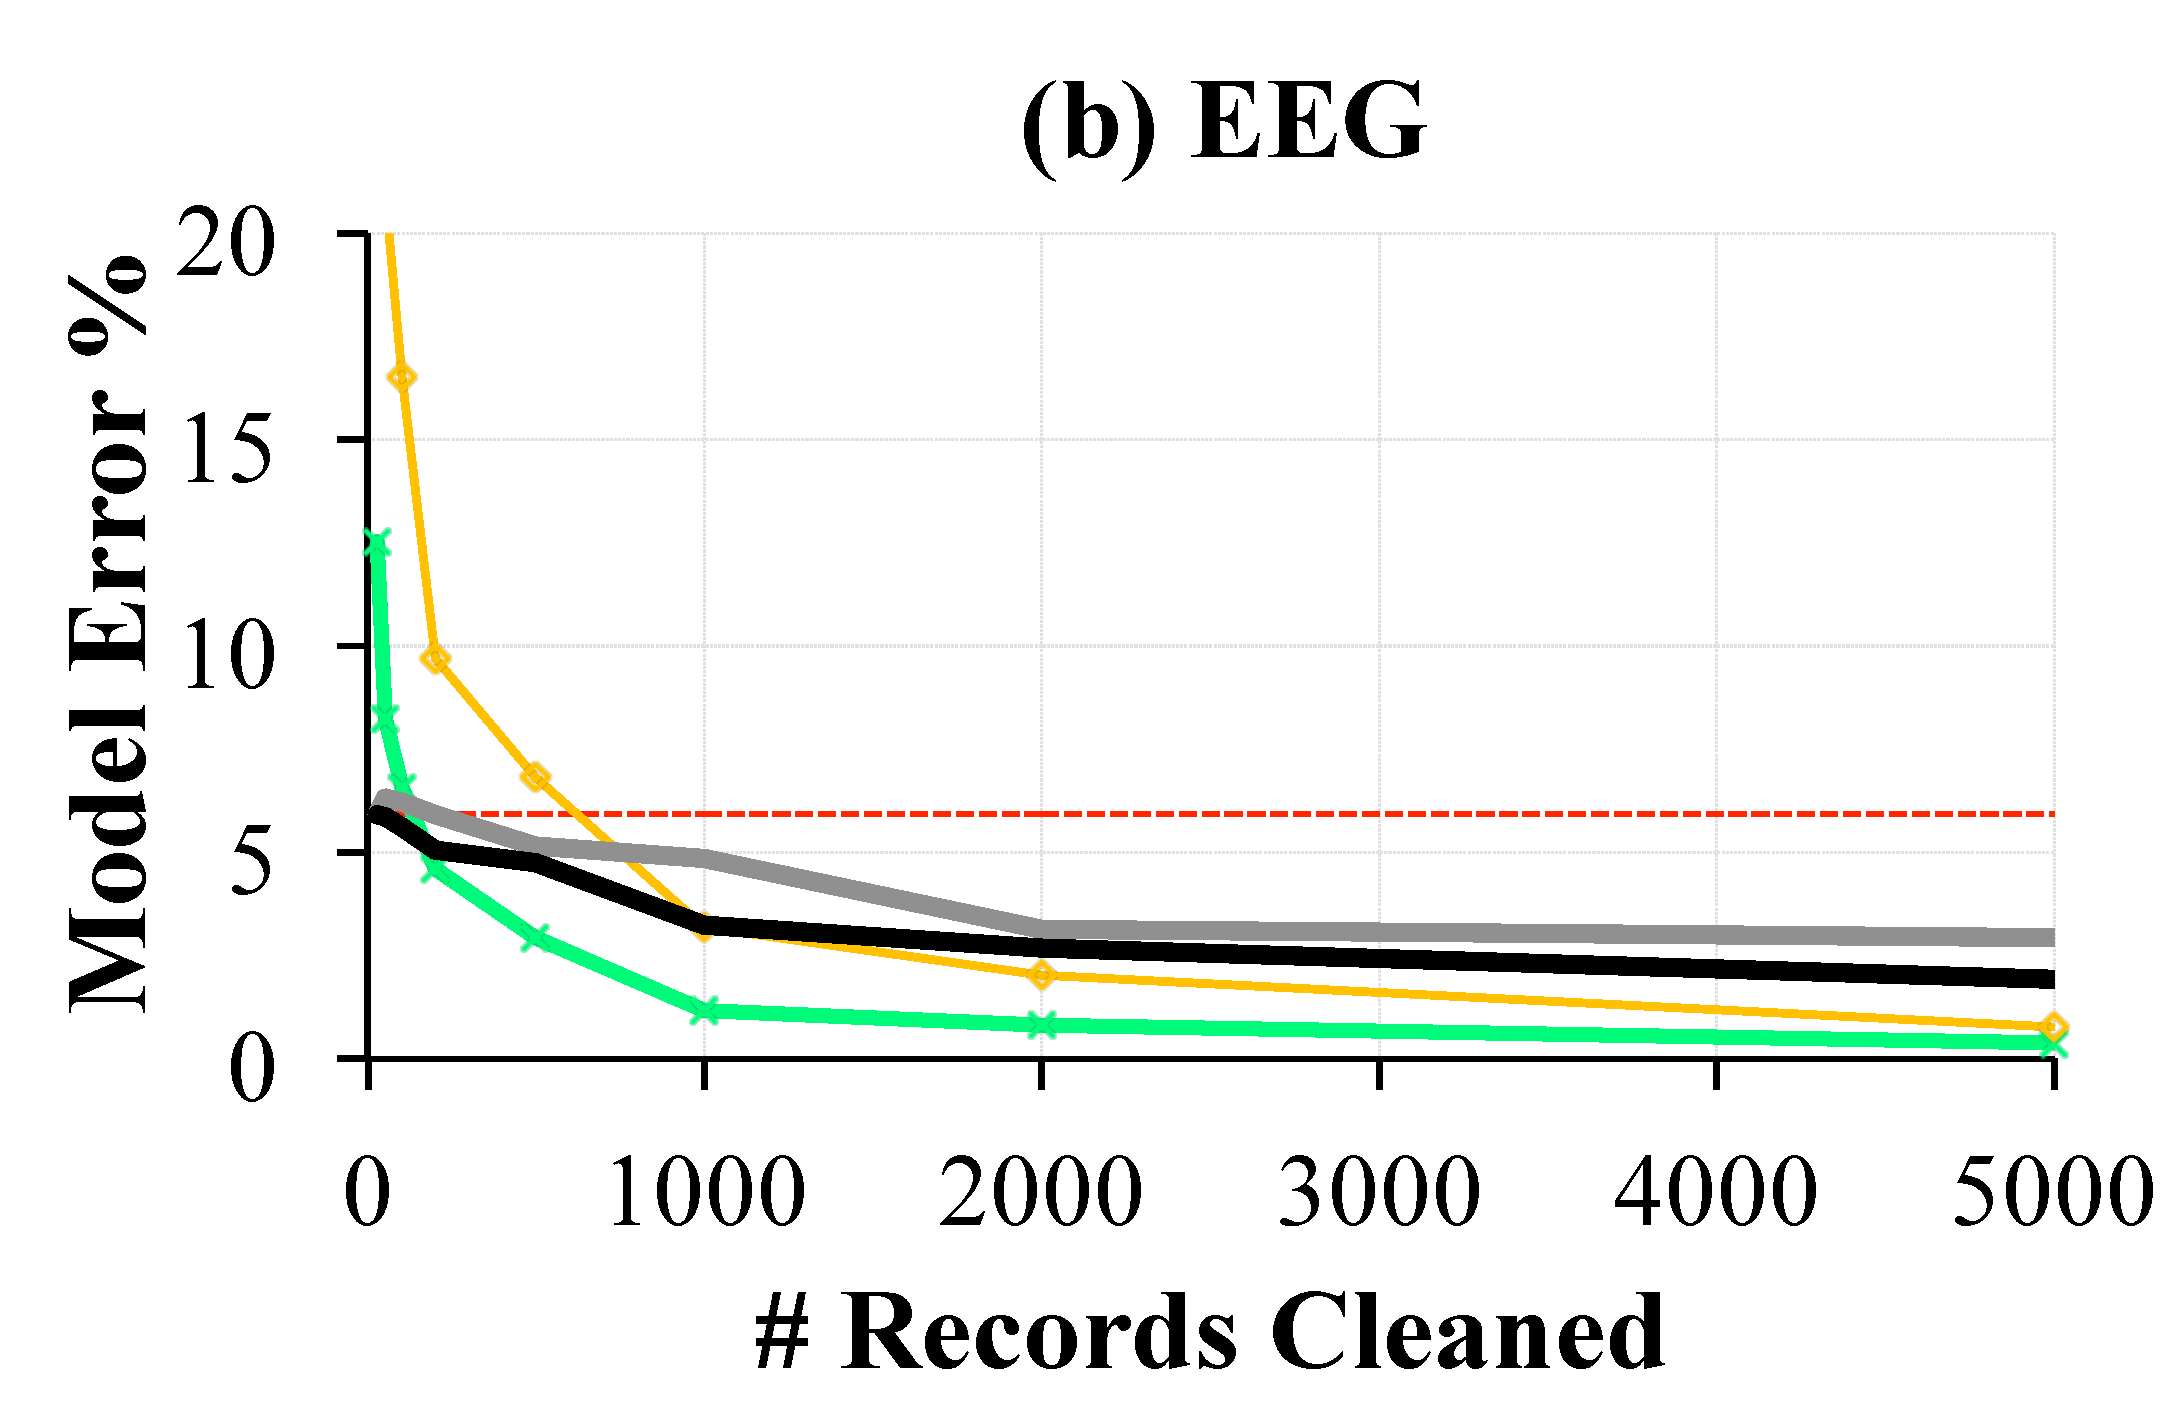
\includegraphics[width=0.49\columnwidth]{exp/exp14b.pdf}
    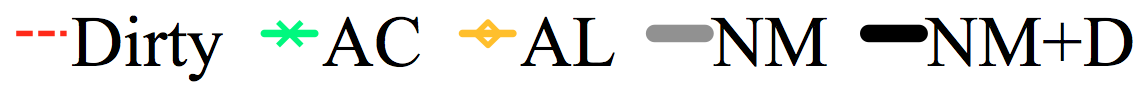
\includegraphics[width=0.49\columnwidth]{exp/legend-14.png}
 \caption{The relative model error as a function of the number of examples cleaned. \sys converges with a smaller sample size to the true result in comparison to partial cleaning (NM, NM+D).  \label{pc-perf}}
\end{figure}

\subsubsection{Corruption Rate}
This experiment explores the tradeoff between Naive-Sampling and \sys.
Figure \ref{bias} varies the systematic corruption rate and plots the number of records examined to achieve 1\% relative error for Naive-Sampling and \sys.
Naive-Sampling does not use the dirty data and thus its error is essentially governed by the the sample size and not the magnitude or prevalence of corruption.
Naive-Sampling outperforms \sys only when corruptions are very severe (45\% in Adult and nearly 60\% in EEG).
When the initialization with the dirty model is inaccurate, \sys does not perform as well. 

\begin{figure}[t]
\centering
 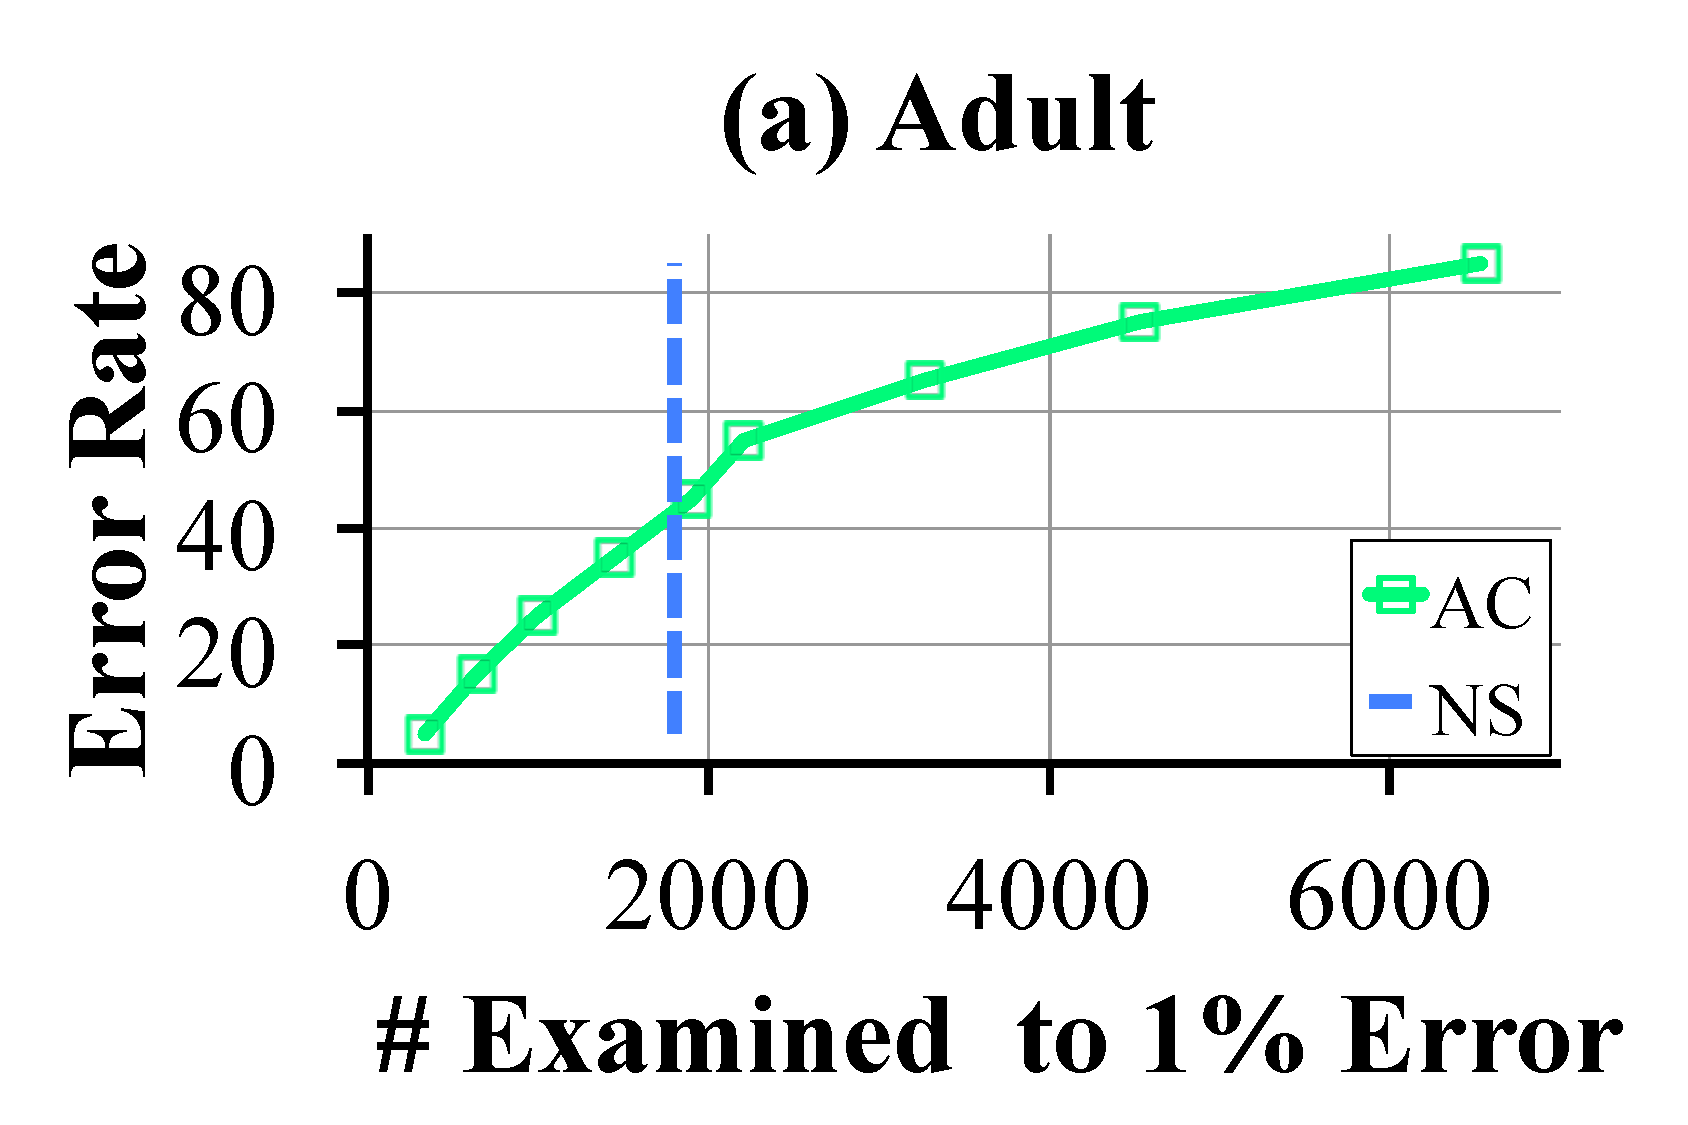
\includegraphics[width=0.49\columnwidth]{exp/exp9a.pdf}
  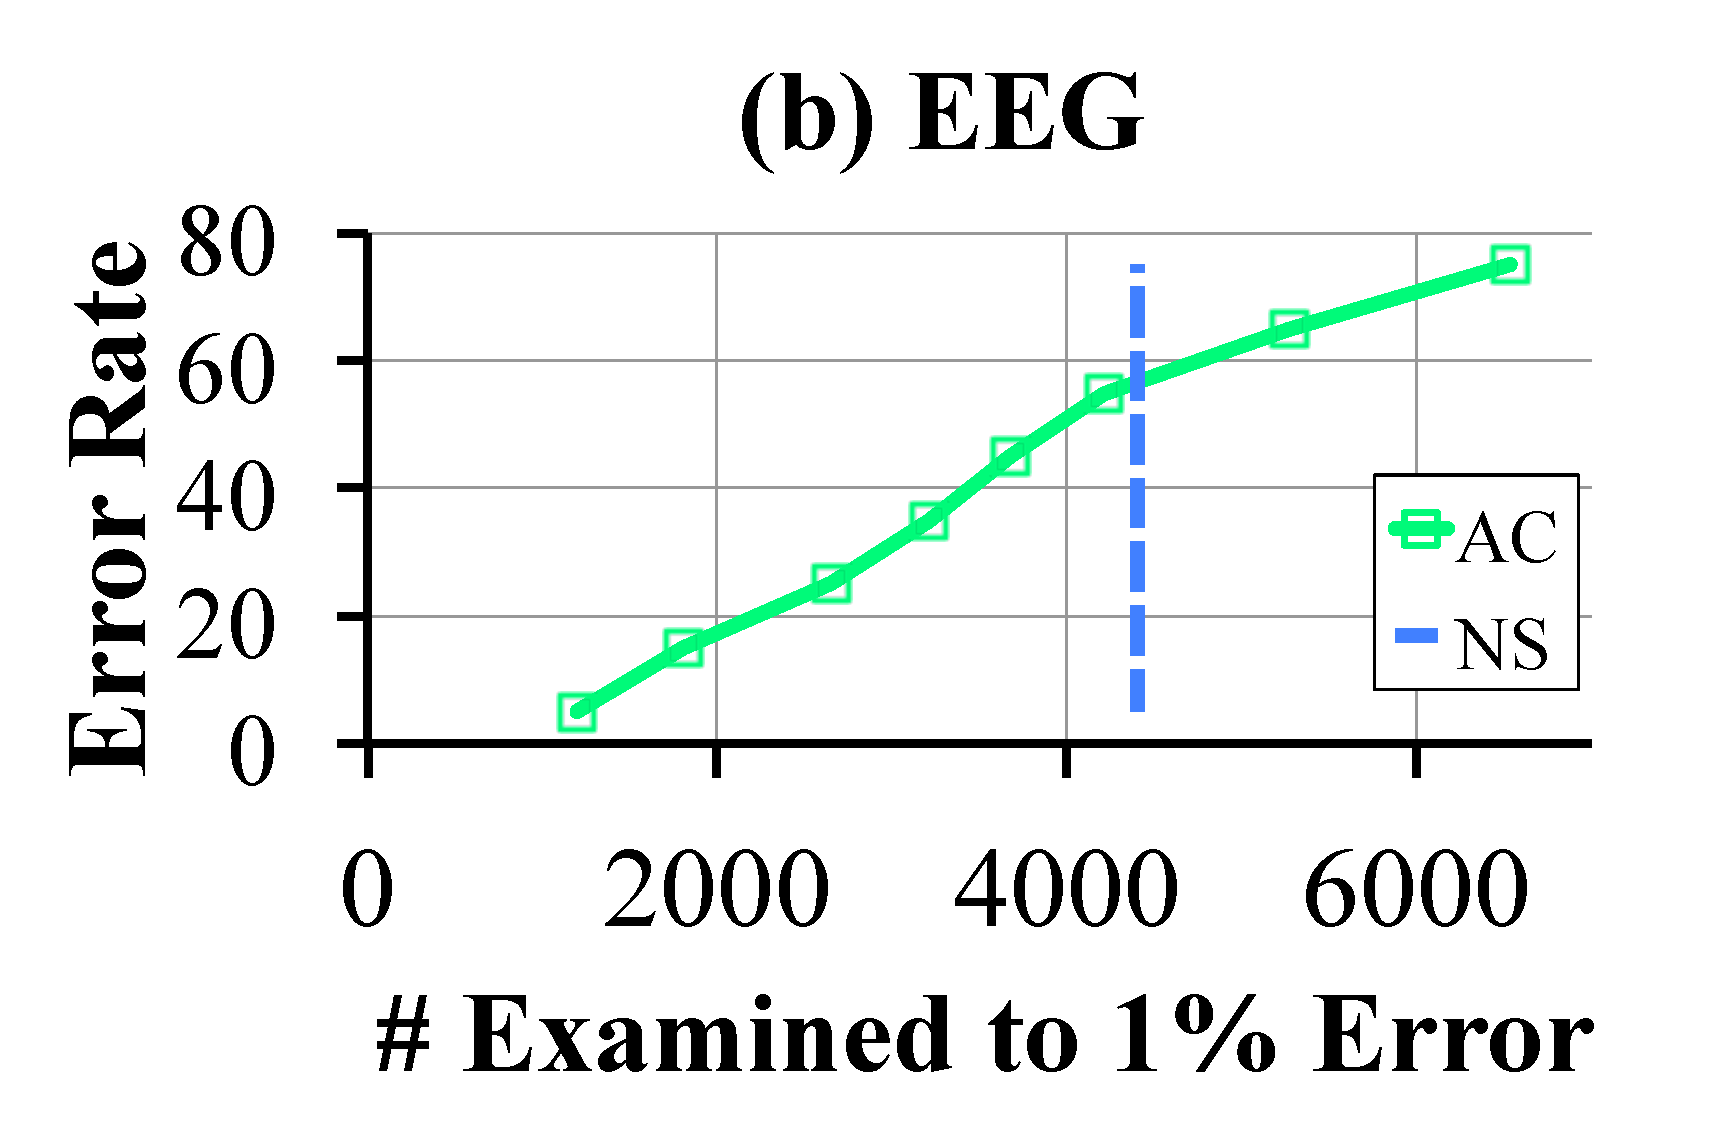
\includegraphics[width=0.49\columnwidth]{exp/exp9b.pdf}
 \caption{\sys outperforms Naive until the corruption is so severe that the dirty model is initialized very far away from the clean model.
  The error of Naive-Sampling does not depend on the corruption rate so it is a vertical line.  \label{bias}}
\end{figure}

\iffalse
\begin{figure}[t]
\centering\vspace{-1em}
 %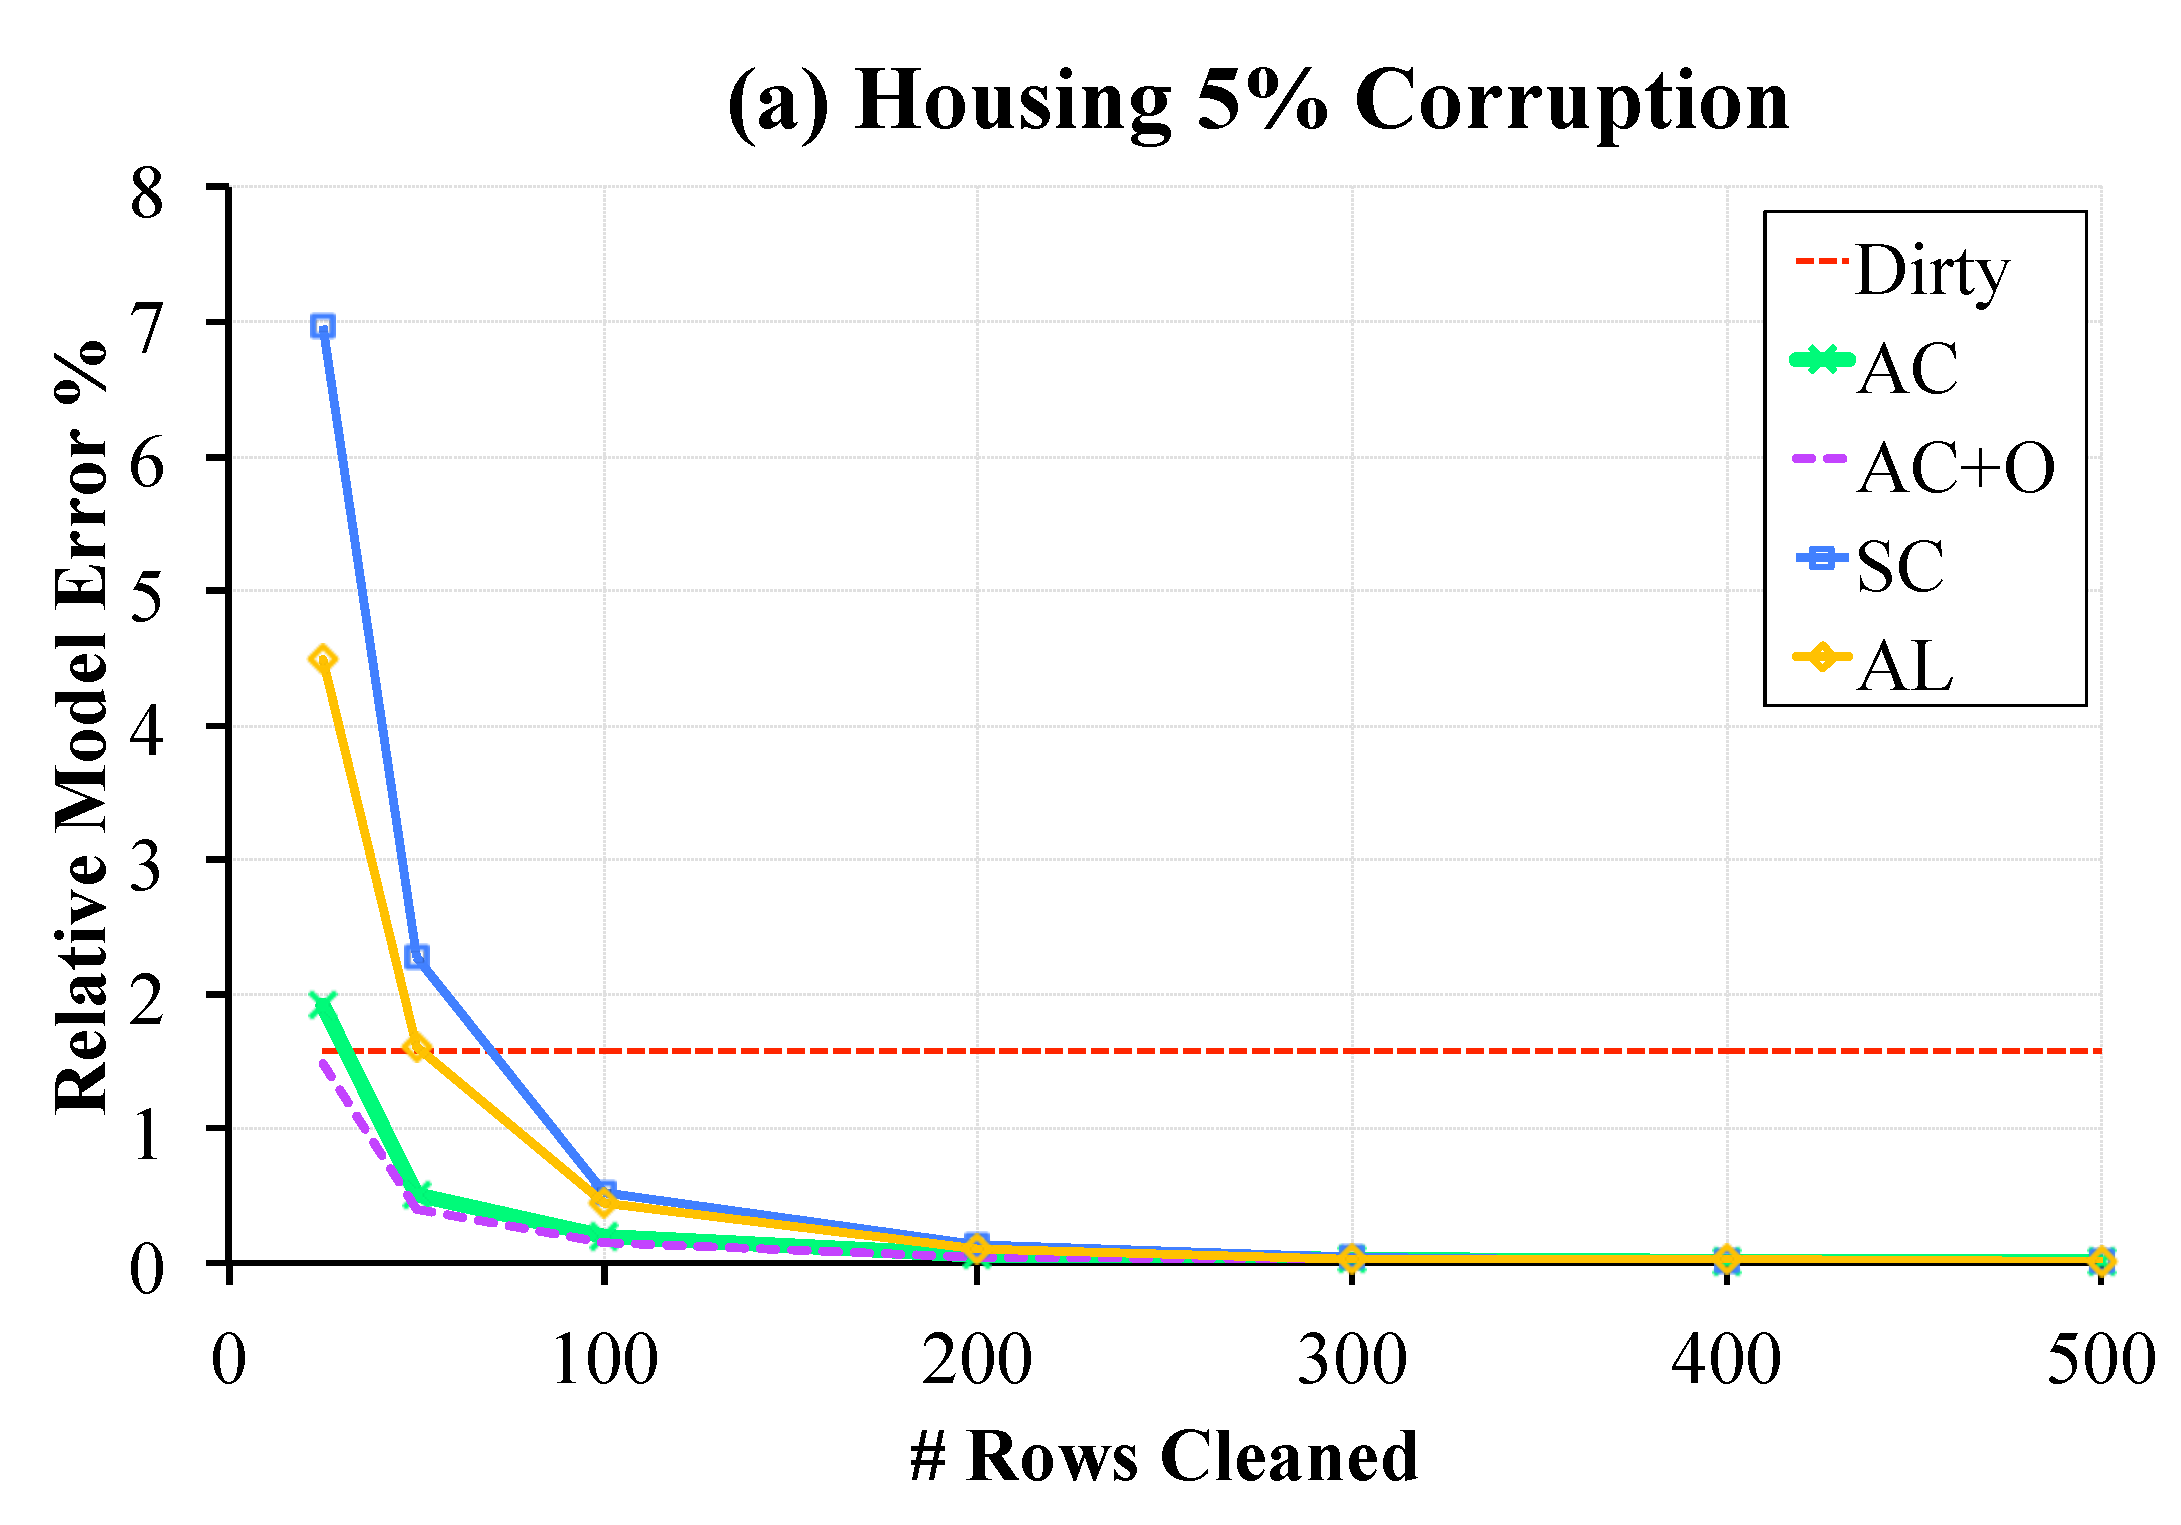
\includegraphics[scale=0.15]{exp/exp3a.pdf}
 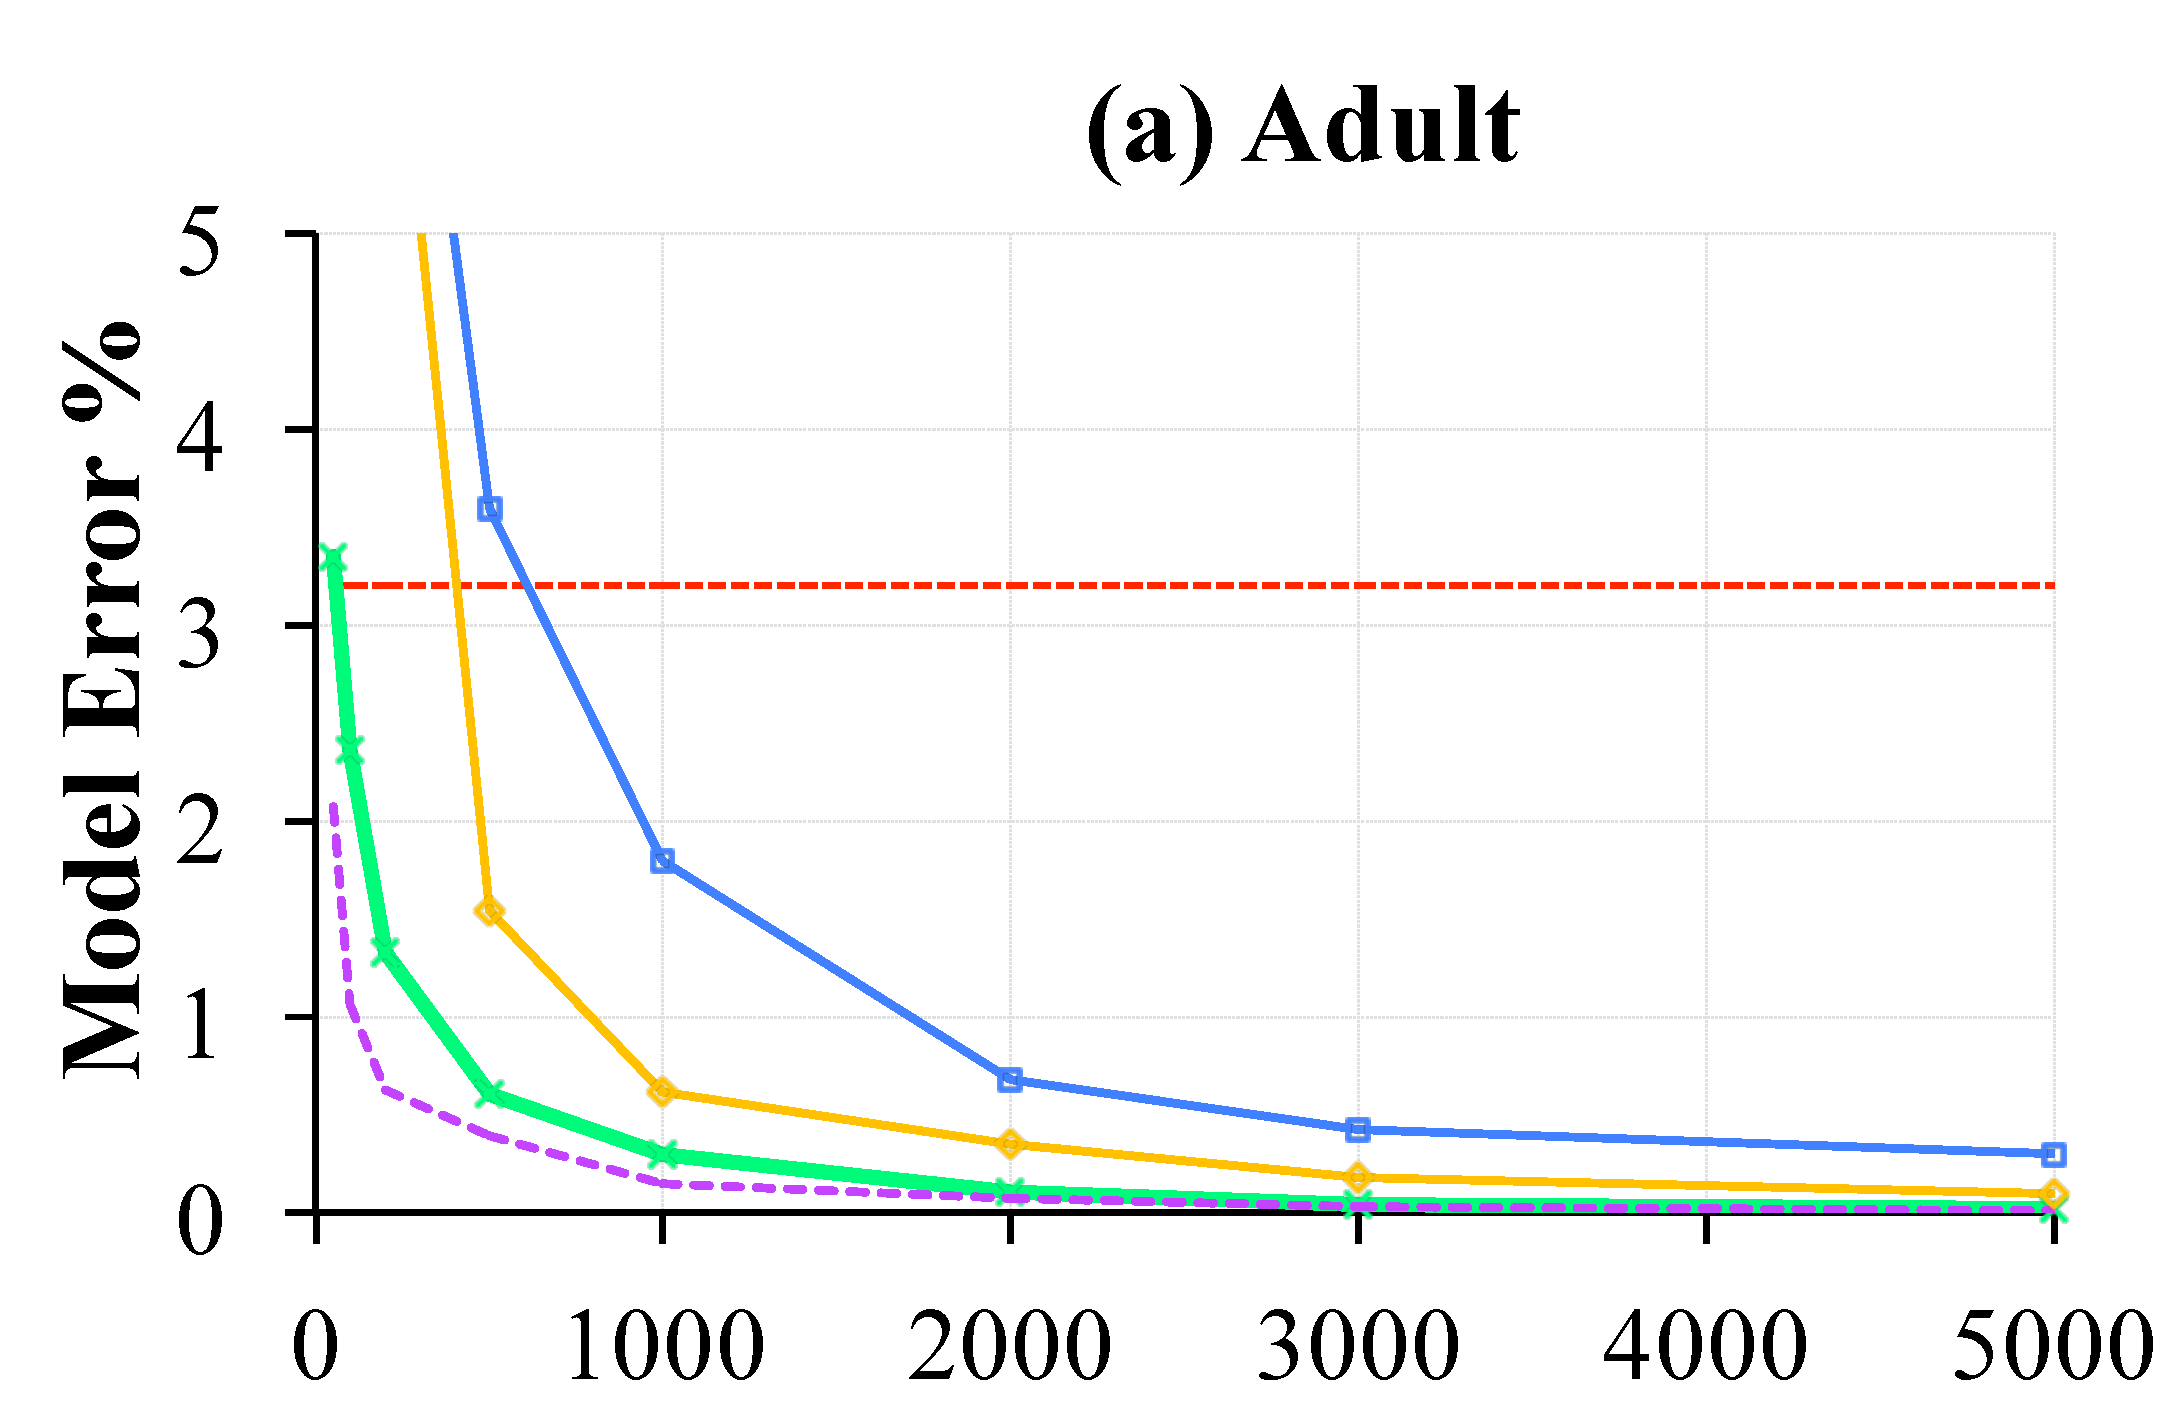
\includegraphics[width=0.49\columnwidth]{exp/exp3b.pdf}
  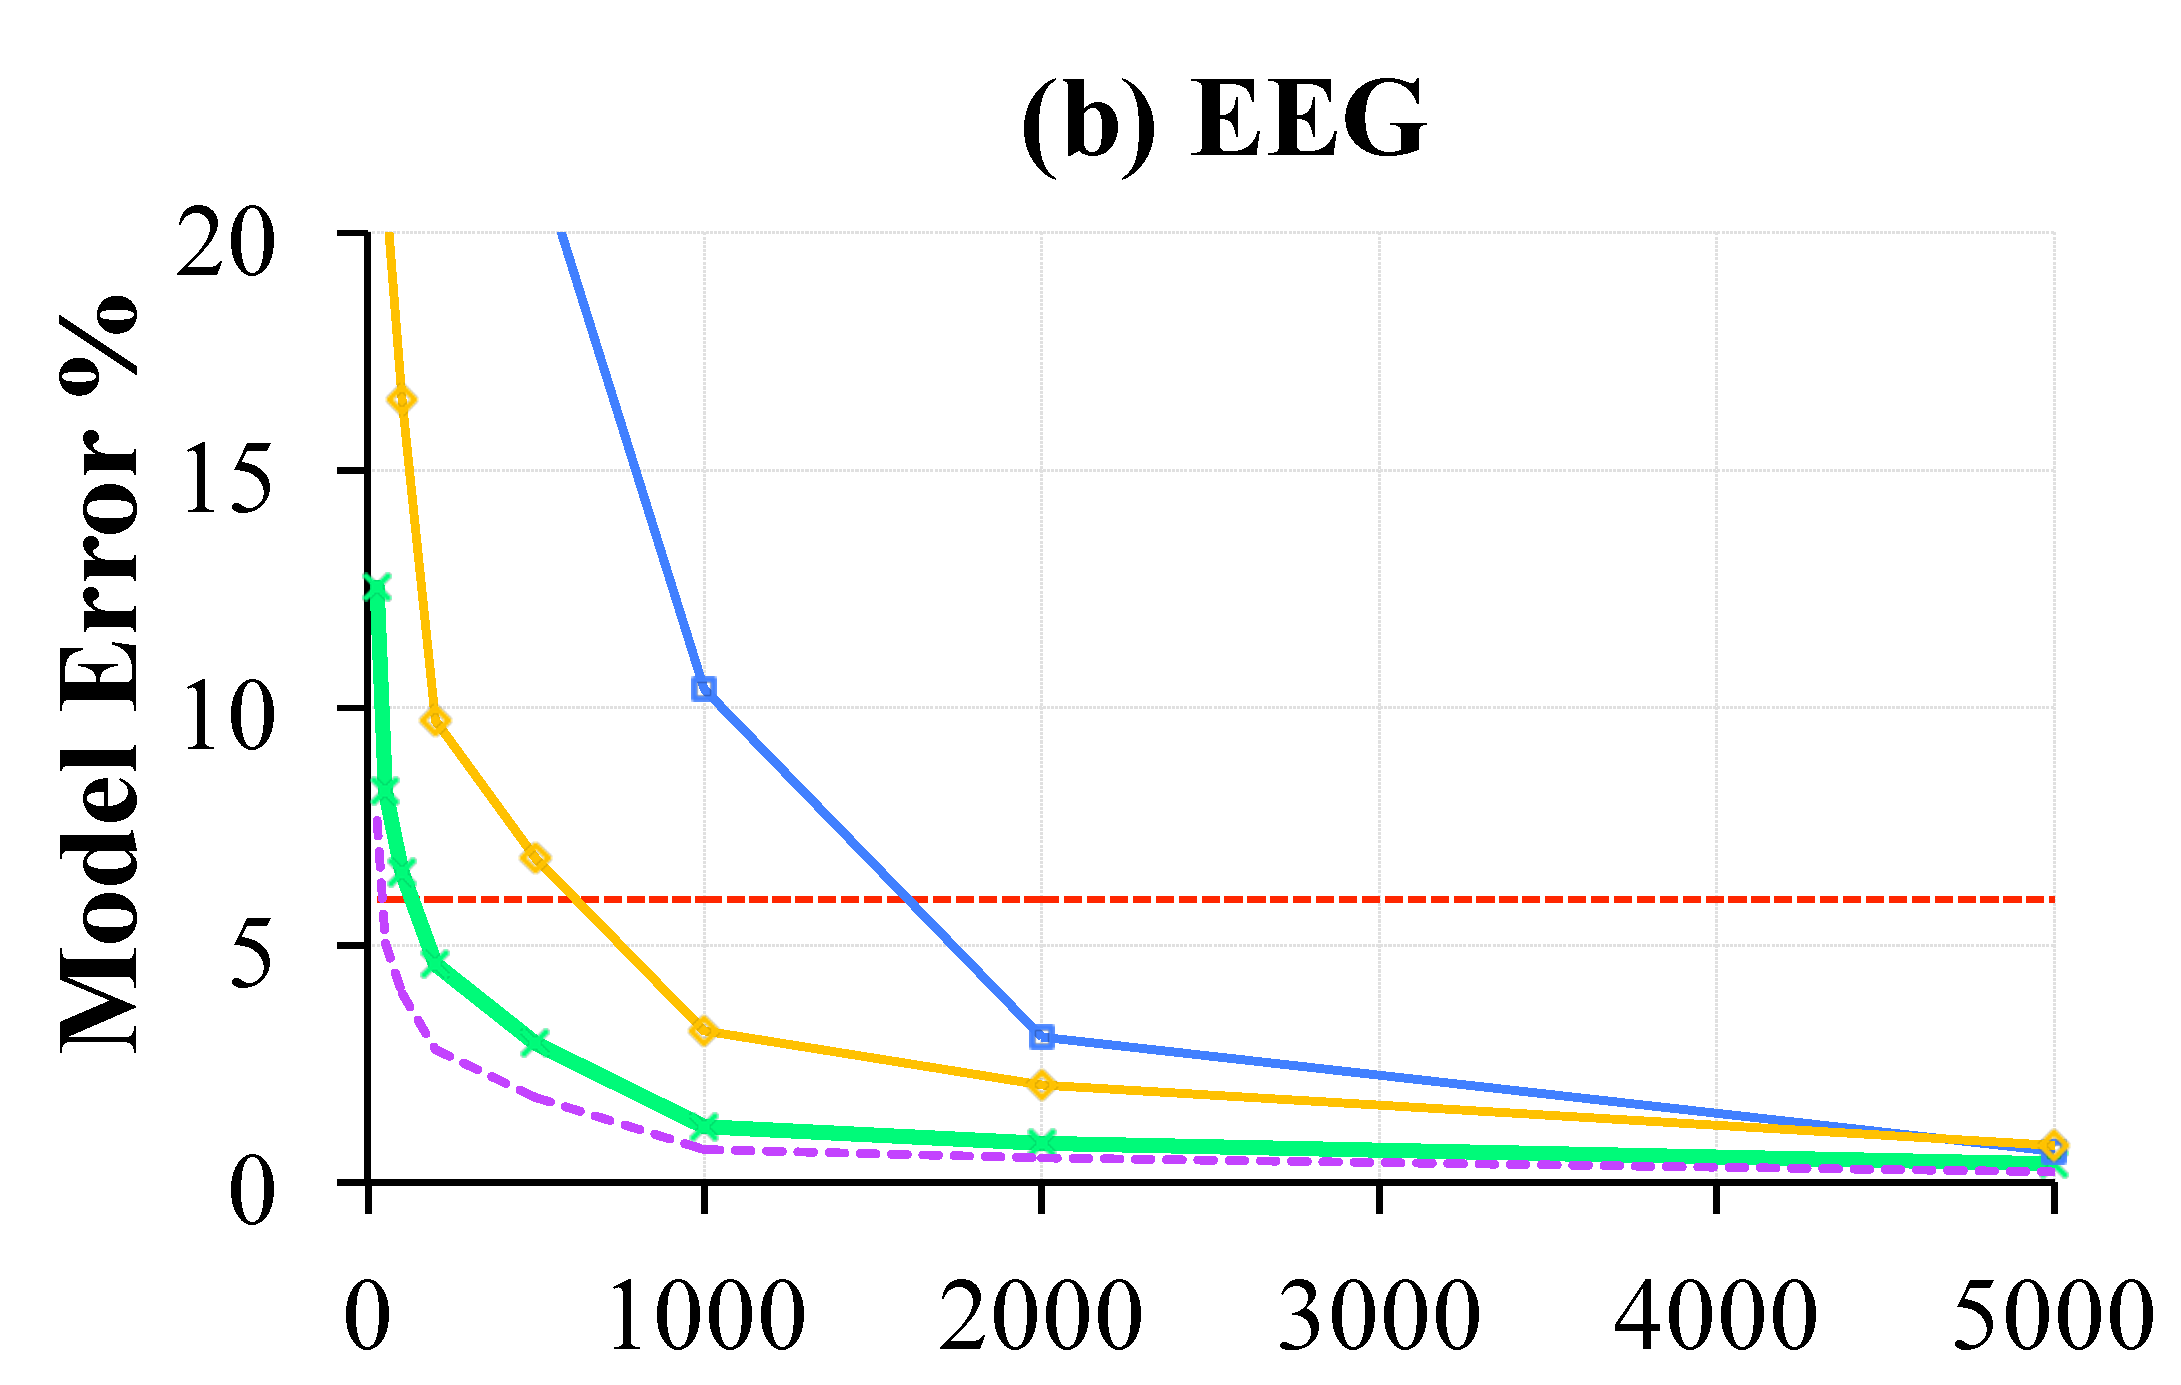
\includegraphics[width=0.49\columnwidth]{exp/exp3c.pdf}
  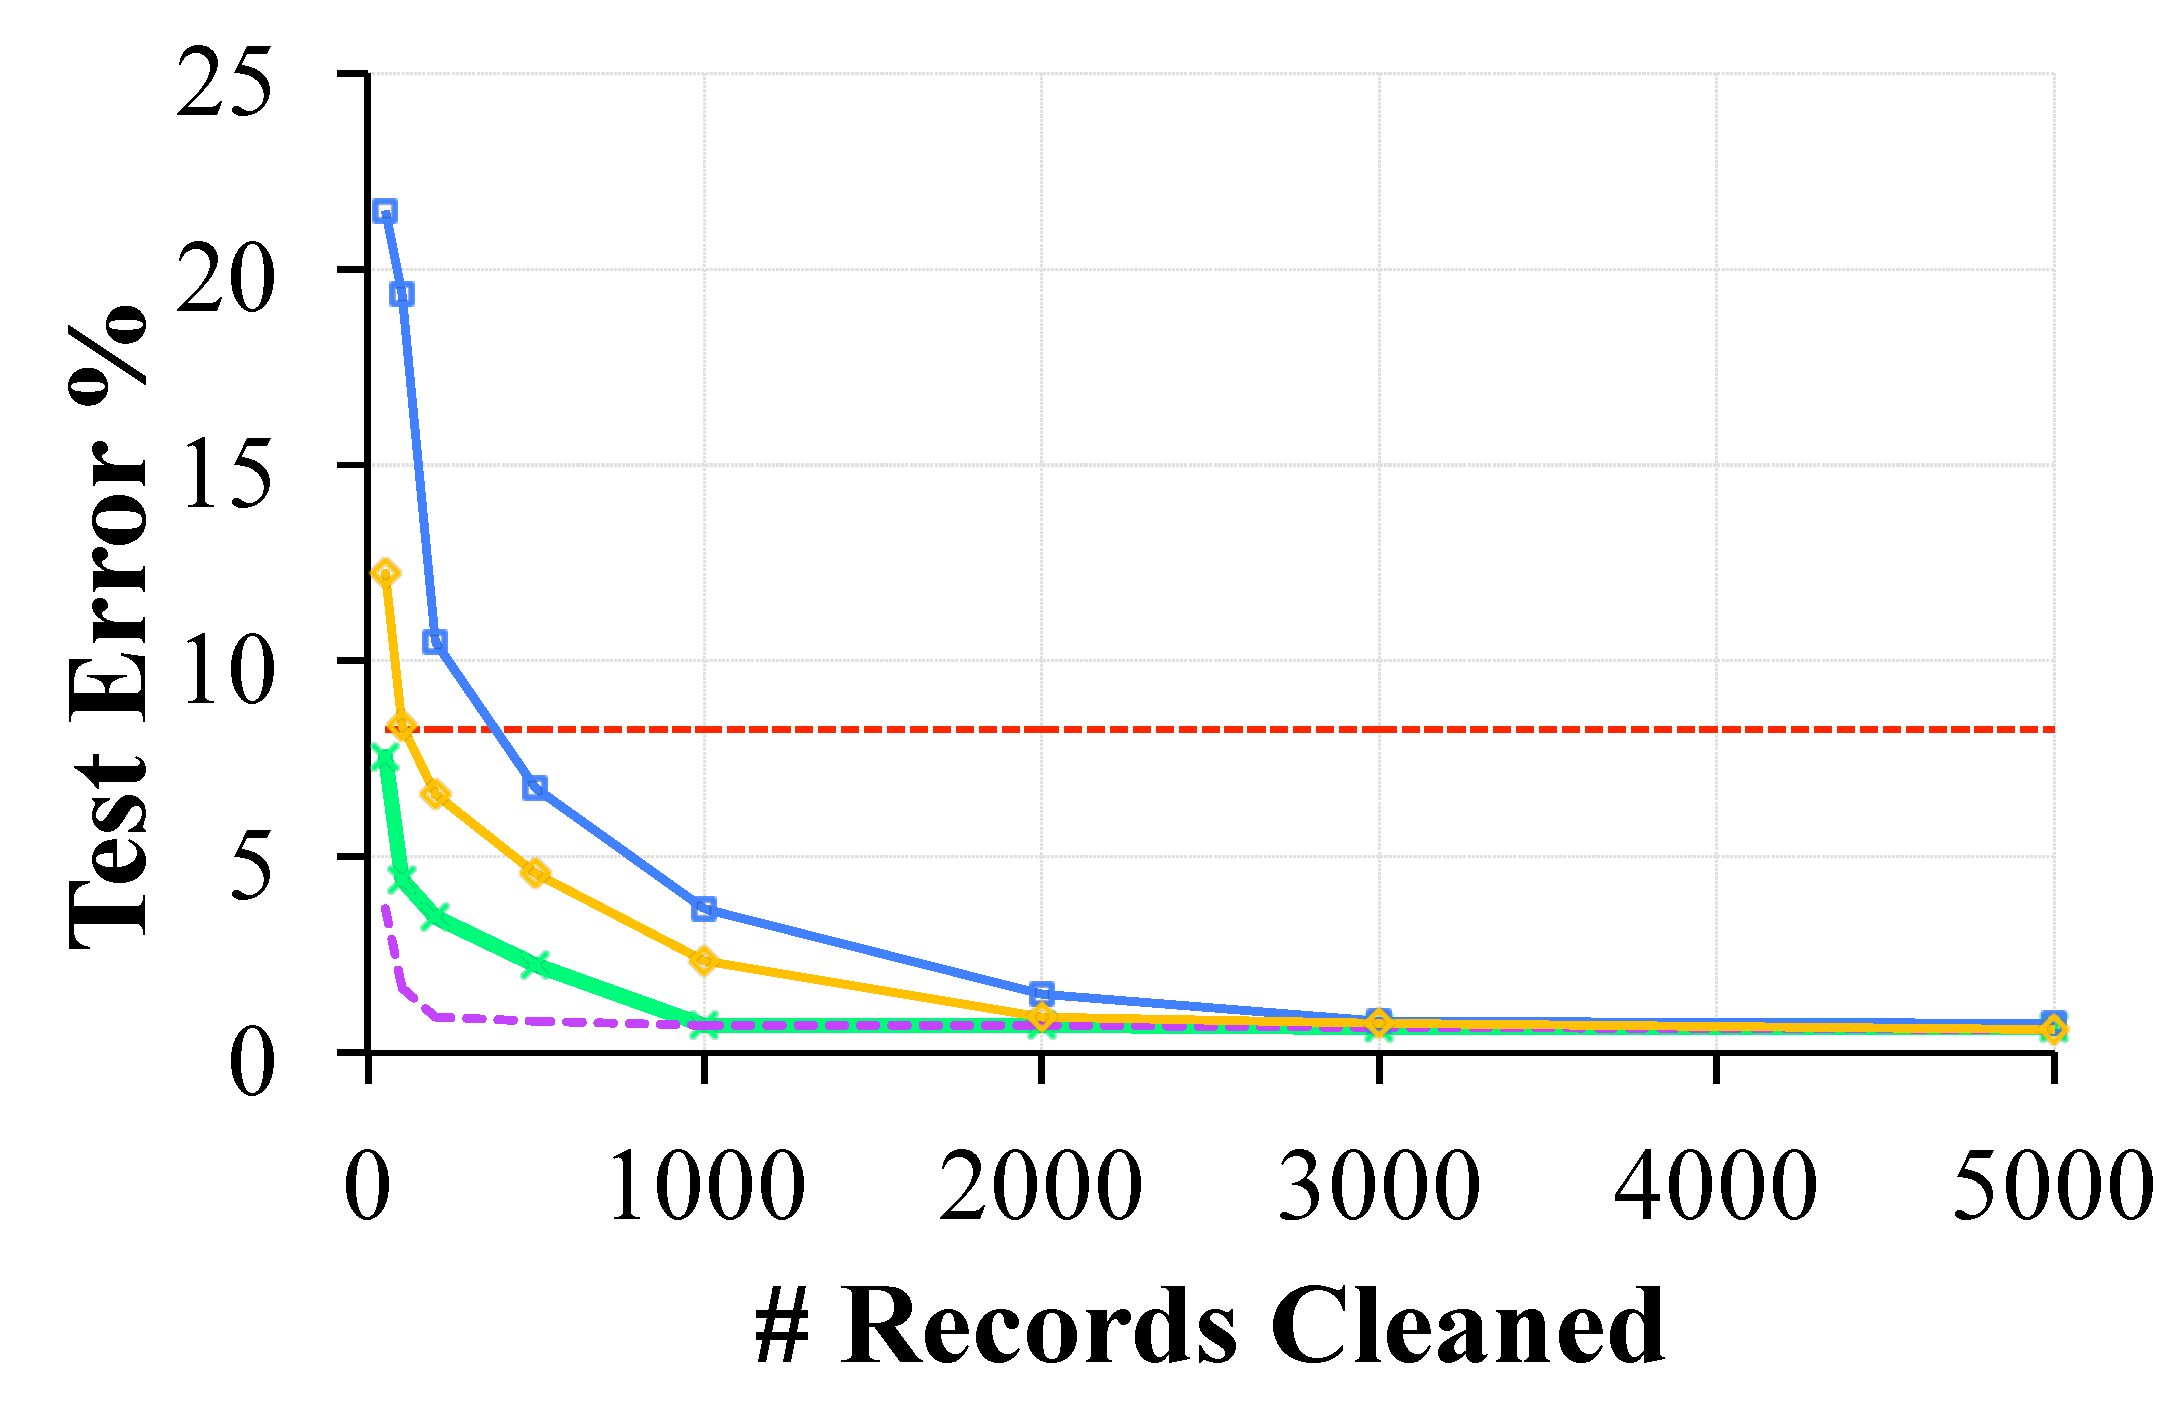
\includegraphics[width=0.49\columnwidth]{exp/exp3bb.pdf}
  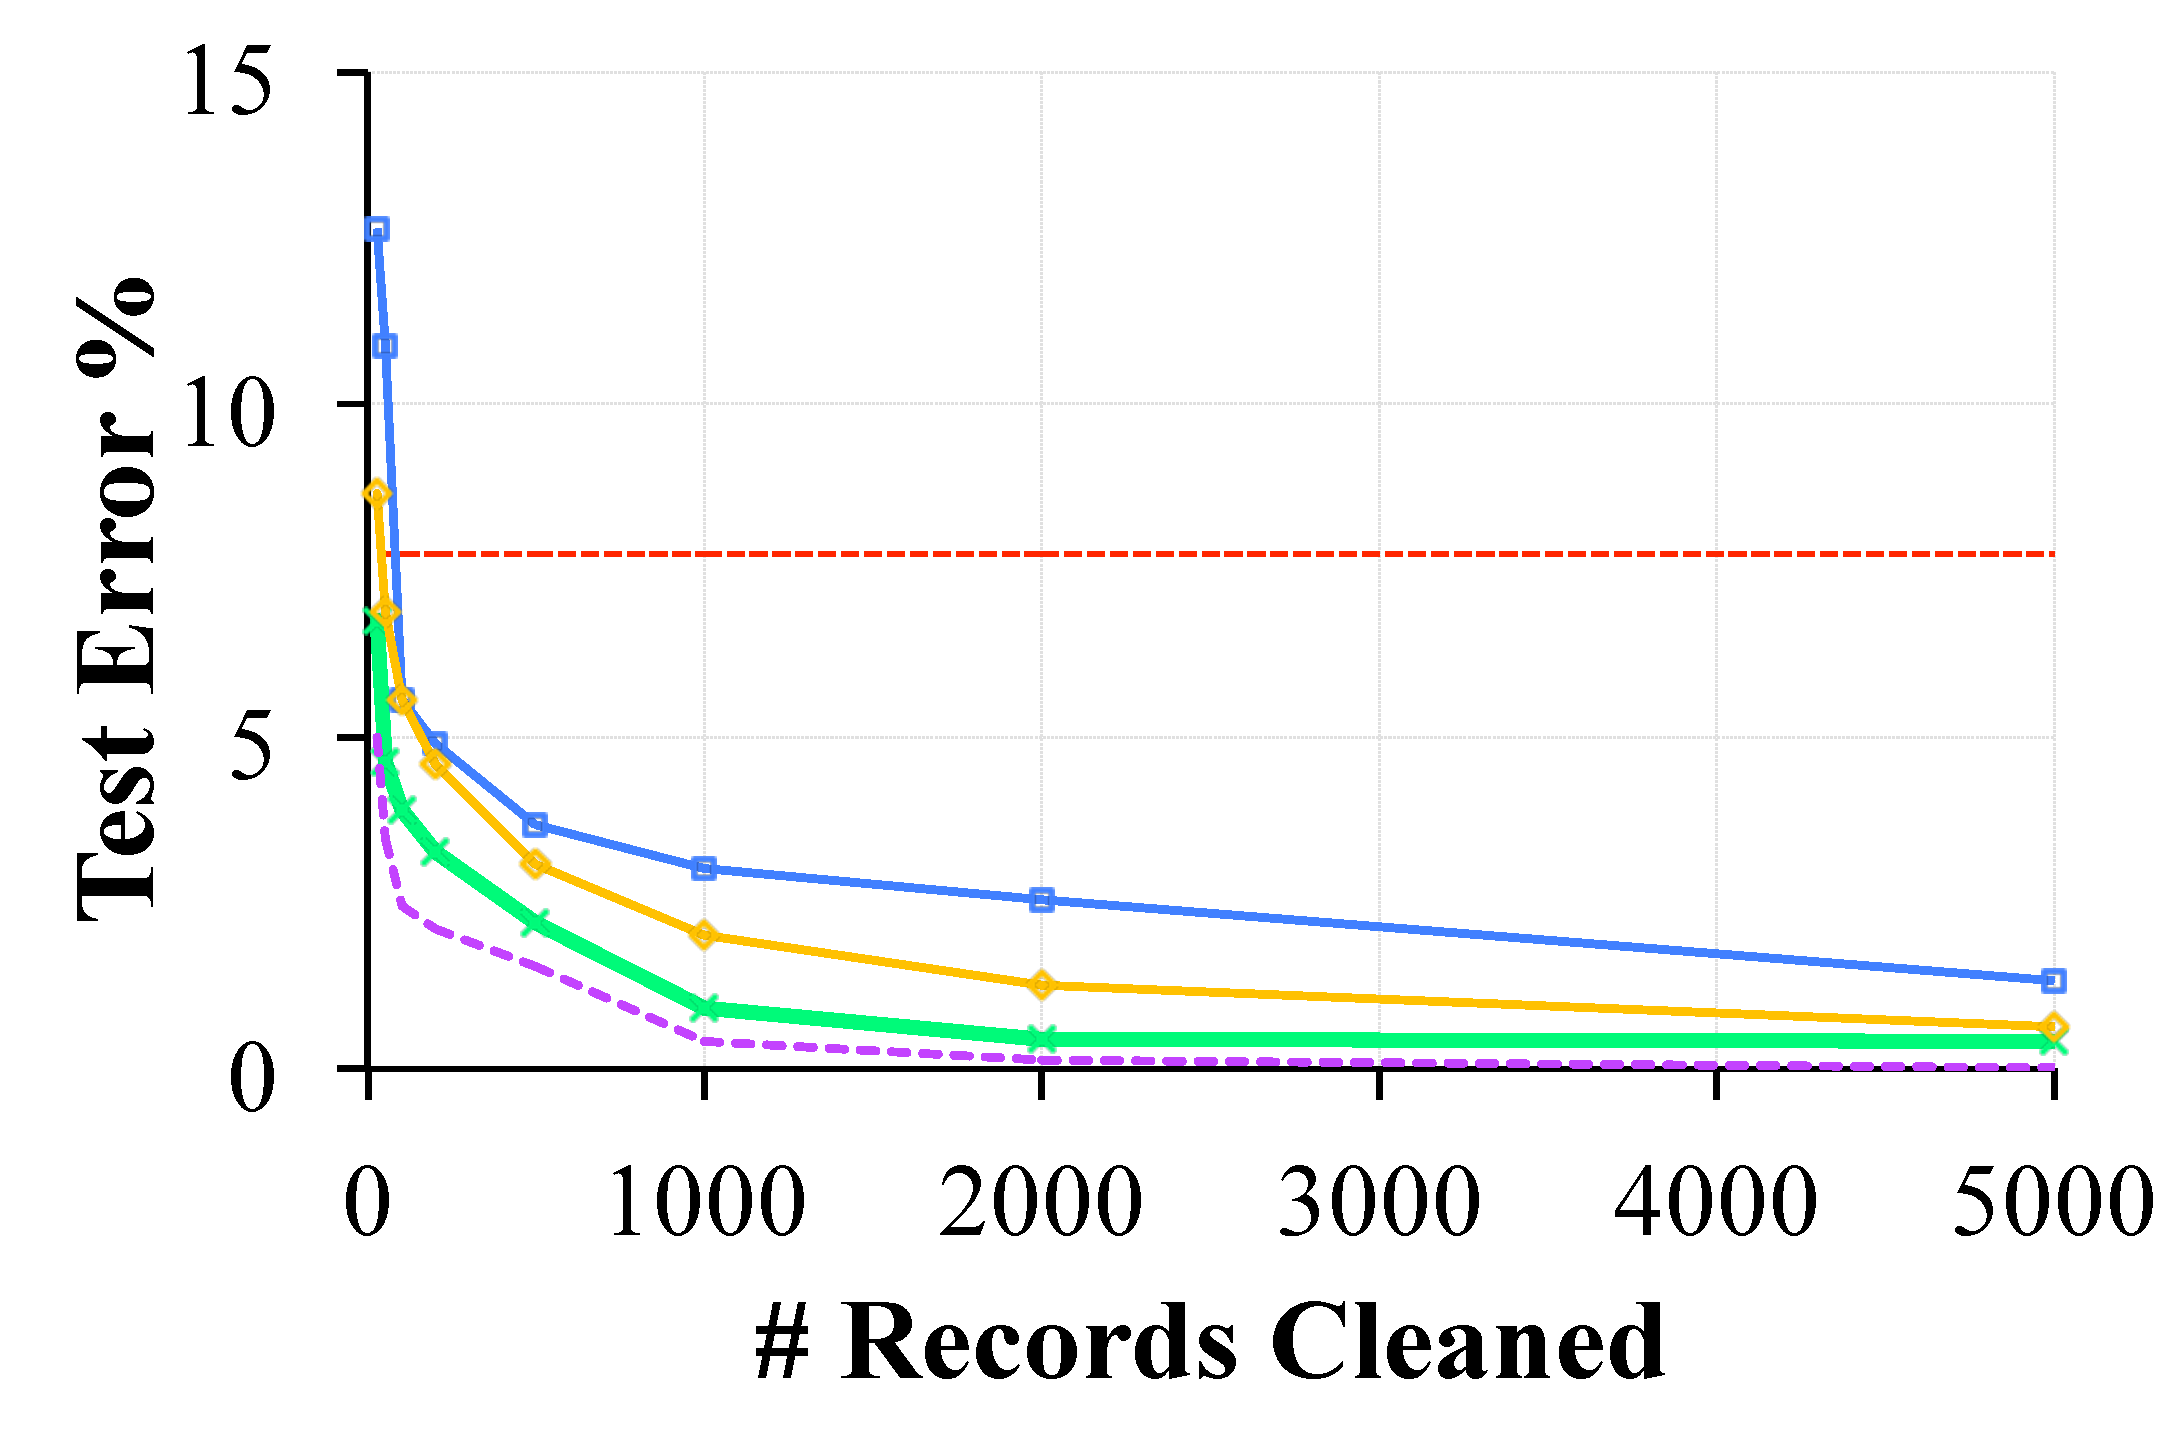
\includegraphics[width=0.49\columnwidth]{exp/exp3cc.pdf}
  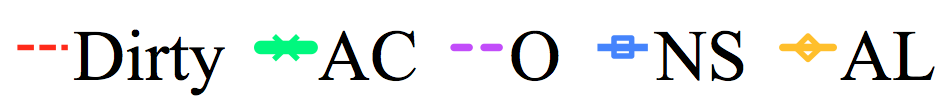
\includegraphics[width=0.5\columnwidth]{exp/legend-general.png}
 \caption{ The relative model error as a function of the number of examples cleaned. \sys converges with a smaller sample size to the true result in comparison to Active Learning and Naive-Sampling. \label{prio-perf}}
\end{figure}

\subsubsection{Samples-to-Error}
This experiment evaluates the samples-to-error tradeoff between four alternative algorithms: \sys (AC), SampleClean, Active Learning, and \sys+Oracle (AC+O).
Figure \ref{prio-perf} shows the model error and test accuracy as a function of the number of cleaned records.
In terms of model error, \sys gives its largest benefits for small sample sizes.
For 500 cleaned records of the Adult dataset, \sys has 6.1x less error than SampleClean and 2.1x less error than Active Learning.
For 500 cleaned records of the EEG dataset, \sys has 9.6x less error than SampleClean and 2.4x less error than Active Learning.
Both Active Learning and \sys benefit from the initialization with the dirty model as they do not retrain their models from scratch, and \sys improves on this performance with detection and error estimation.
Active Learning has no notion of dirty and clean data, and therefore prioritizes its selections with respect to the dirty data.
These gains in model error also correlate well to improvements in test error (defined as the test accuracy difference w.r.t cleaning all data).
The test error converges more quickly than model error, emphasizing the benefits of progressive data cleaning since it is not necessary to clean all the data to get a model with essentially the same performance as the clean model.
For example, to achieve a test error of 1\% on the Adult dataset, \sys cleans 500 fewer records than Active Learning.
\fi

\subsubsection{Dirty Data Detection}
Adaptive detection depends on predicting which records are dirty; and this is again related to the systematic nature of data error.
For example, random corruption not correlated with any other data features may be hard to learn.
As corruption becomes more random, the classifier becomes increasingly erroneous.
This experiment explores making our generated systematic corruption incrementally more random.
Instead of selecting the highest valued records for the most valuable features, we corrupt random records with probability $p$. 
We compare these results to AC-D where we do not have a detector at all (for a fixed number of 1000 records examined).
Figure \ref{tradeoffs2}a plots the relative error reduction using a classifier.
When the corruption is about 50\% random then there is a break even point where no detection is better.
The classifier is imperfect and misclassifies some data points incorrectly as cleaned.

\begin{figure}[t]
\centering
 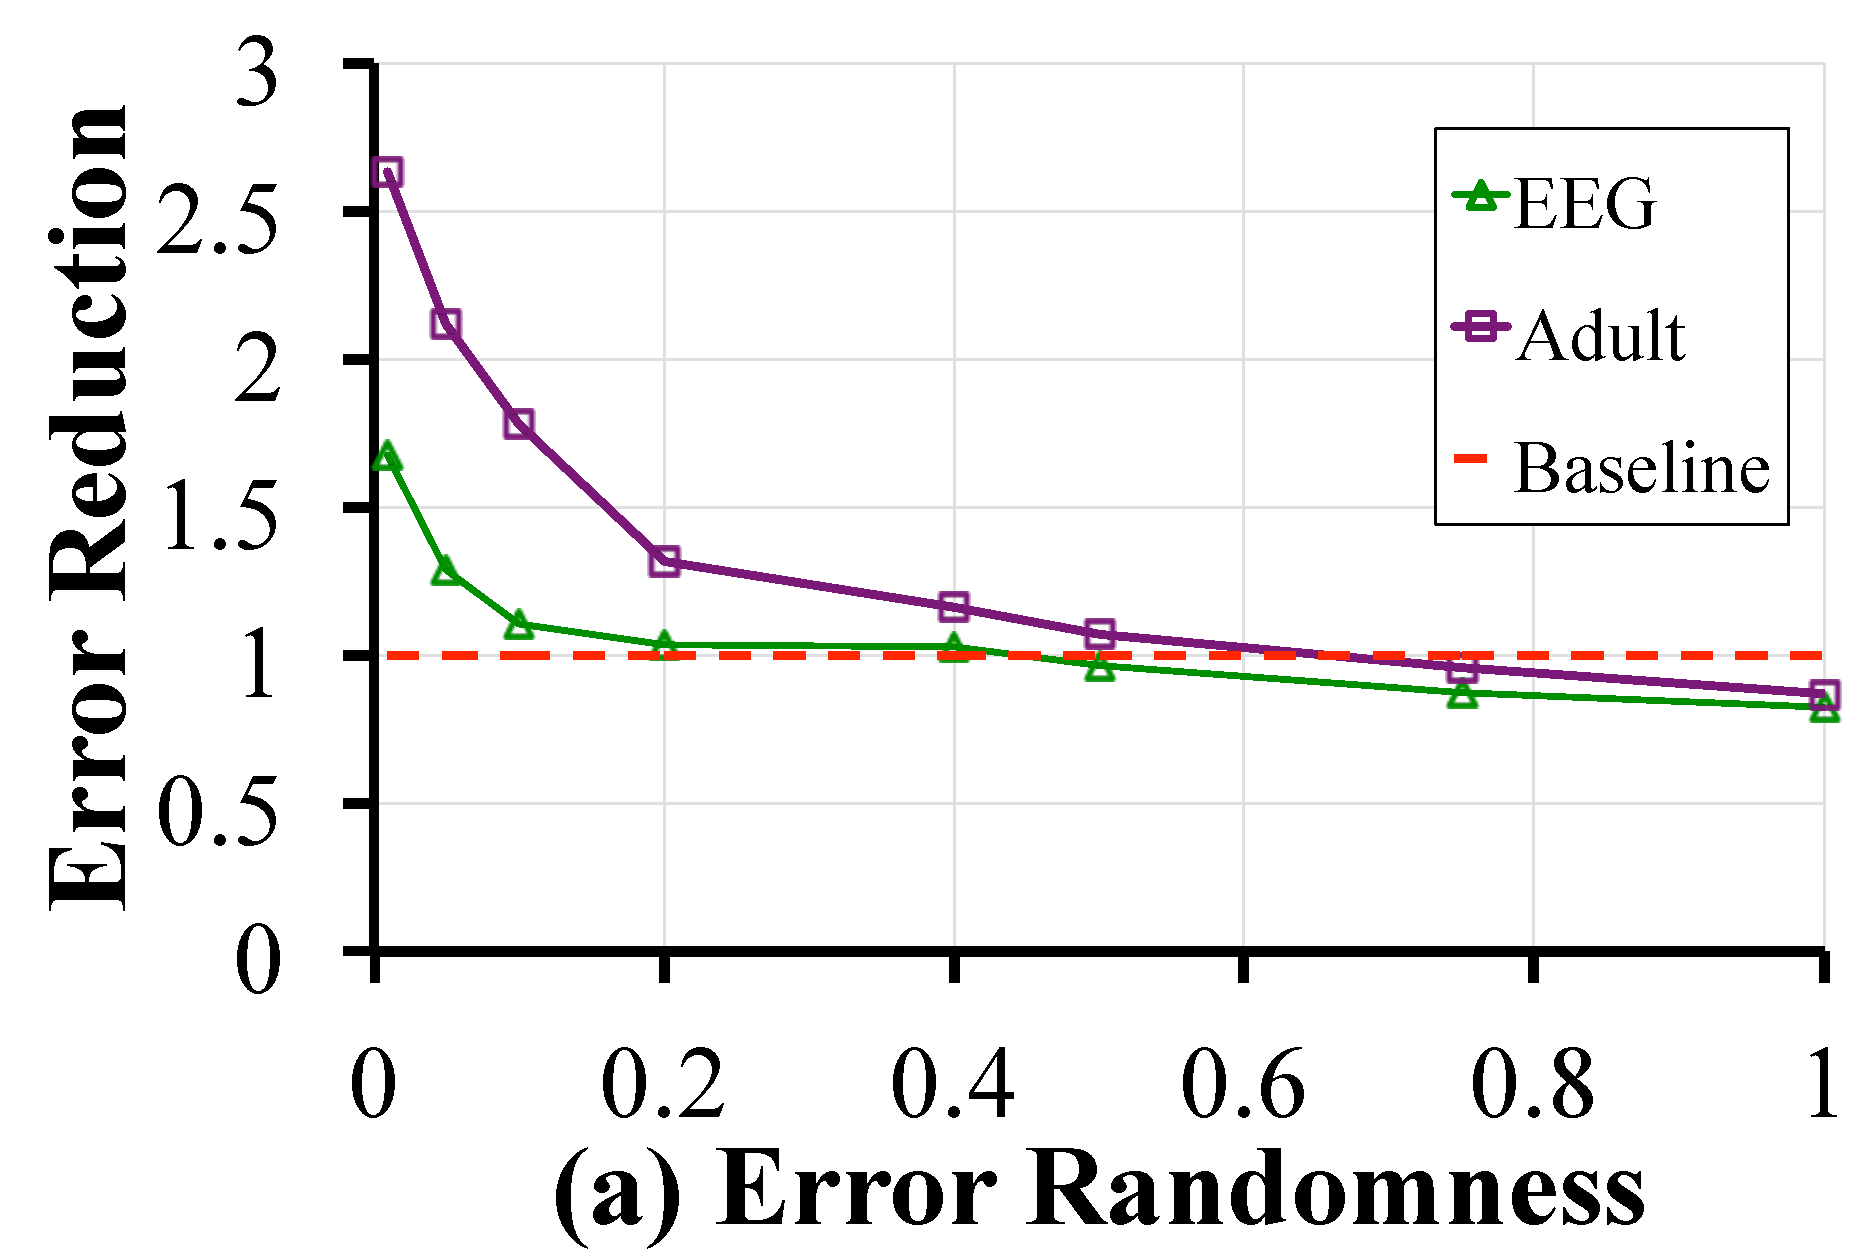
\includegraphics[width=0.49\columnwidth]{exp/exp5a.pdf}
 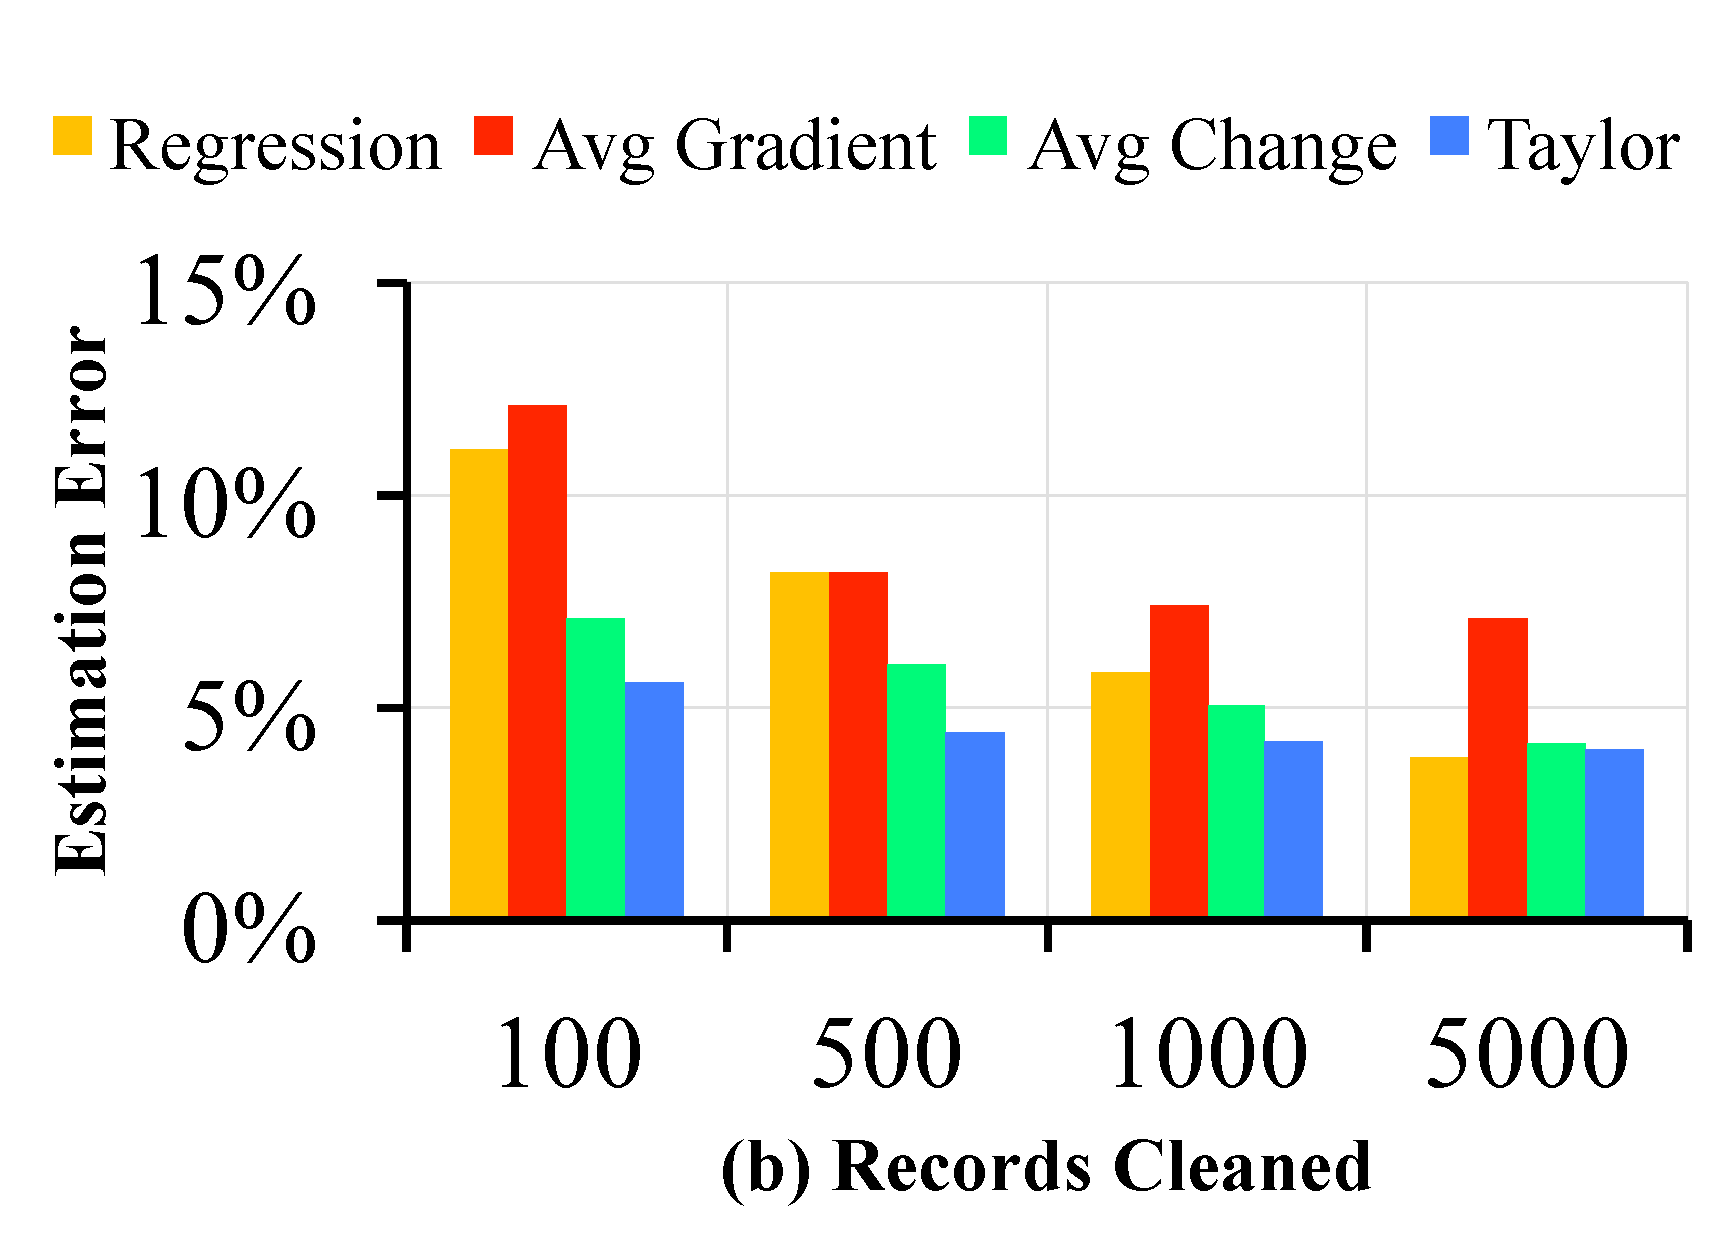
\includegraphics[width=0.49\columnwidth]{exp/exp12.pdf}
 \caption{(a) Data corruptions that are less random are easier to classify, and lead to more significant reductions in relative model error. (b) The Taylor series approximation gives more accurate estimates when the amount of cleaned data is small. \label{tradeoffs2}}
\end{figure}

\subsubsection{Impact Estimation}\label{est}
This experiment compares estimation techniques: (1) ``linear regression" trains a linear regression model that predicts the clean gradient as a function of the dirty gradient, (2) ``average gradient" which does not use the detection to inform how to apply the estimate, (3) ``average feature change" uses detection but no linearization, and (4) the Taylor series linear approximation.
Figure \ref{tradeoffs2}b measures how accurately each estimation technique estimates the gradient as a function of the number of examined records on the EEG dataset.
Estimation error is measured using the relative L2 error with the true gradient.
The Taylor series approximation proposed gives more accurate for small cleaning sizes.

\iffalse
\subsection{Summary of Experiments}
In summary, we evaluated \sys on five datasets with both real and synthetic corruption. We find that when data error is systematic \sys can train models with a fraction of the cleaning effort of alternative techniques.
On the two real datasets, from IMDB and ProPublica, we found that many types of corruption are indeed systematic.
We also showed that our proposed optimizations (detection and sampling) further reduce cleaning effort by up-to 2.5x, and we characterized the limitations of \sys (a model trained on the dirty data is a poor initialization).
We have been noted this in our prior work on other datasets as well, where corruption is correlated with the hypotheses of interest~(see Microsoft Academic Search in~\cite{wang1999sample}, see World Bank in~\cite{activecleanarxiv}). 
However, it is possible that some types of errors do not have a systematic bias; however, the analyst could not know this for certain without applying a tool like \sys.
\fi



\section{Related Work}\label{rw}
\noindent \textbf{Data Cleaning: } 
There are a number of other works that use machine learning to improve the efficiency and/or reliability of data cleaning~\cite{DBLP:journals/pvldb/YakoutENOI11,yakout2013don,gokhale2014corleone}.
For example, Yakout et al. train a model that evaluates the likelihood of a proposed replacement value \cite{yakout2013don}.
Another application of machine learning is value imputation, where a missing value is predicted based on those records without missing values.
Machine learning is also increasingly applied to make automated repairs more reliable with human validation \cite{DBLP:journals/pvldb/YakoutENOI11}.
Human input is often expensive and impractical to apply to entire large datasets.
Machine learning can extrapolate rules from a small set of examples cleaned by a human (or humans) to uncleaned data \cite{gokhale2014corleone, DBLP:journals/pvldb/YakoutENOI11}.
This approach can be coupled with active learning \cite{DBLP:journals/pvldb/MozafariSFJM14} to learn an accurate model with the fewest possible number of examples.
While, in spirit, \sys is similar to these approaches, it addresses a very different problem of data cleaning before user-specified modeling.
%The key new challenge in this problem is ensuring the correctness of the user's model after partial data cleaning.

SampleClean~\cite{wang1999sample} applies data cleaning to a sample of data, and estimates the results of aggregate queries.
Sampling has also been applied to estimate the number of duplicates in a relation \cite{heise2014estimating}. 
Similarly, Bergman et al. explore the problem of query-oriented data cleaning \cite{DBLP:conf/sigmod/BergmanMNT15}, where given a query, they clean data relevant to that query. 
Deshpande et al. studied data acquisition in sensor networks \cite{deshpande2004model}. They explored value of information based prioritization of data acquisition for estimating aggregate queries of sensor readings.
Similarly, Jeffery et al. \cite{DBLP:conf/pervasive/JefferyAFHW06} explored similar prioritization based on value of information.
Existing work does not explore cleaning driven by the downstream machine learning ``queries" studied in this work.
%Finally, incremental optimization methods like SGD have a connection to incremental materialized view maintenance as the argument for incremental maintenance over recomputation is similar (i.e., relatively sparse updates).
%Krishnan et al. explored how samples of materialized views can be maintained similar to how models are updated with a sample of clean data in this work \cite{krishnan2015svc}.

\vspace{0.5em}

\noindent \textbf{Stochastic Optimization and Active Learning: } Zhao and Tong recently proposed using importance sampling in conjunction with stochastic gradient descent \cite{zhao2014stochastic}. 
This line of work builds on prior results in linear algebra that show that some matrix columns are more informative than others \cite{drineas2012fast}, and Active Learning which shows that some labels are more informative that others \cite{settles2010active}.
Active Learning largely studies the problem of label acquisition \cite{settles2010active},
and recently the links between Active Learning and Stochastic optimization have been studied \cite{guillory2009active}. 


\vspace{0.5em}

\noindent \textbf{Transfer Learning and Bias Mitigation: }  
\sys has a strong link to a field called Transfer Learning and Domain Adaptation \cite{pan2010survey}. The basic idea of Transfer Learning is that suppose a model is trained on a dataset $D$ but tested on a dataset $D'$. 
Much of the complexity and contribution of \sys comes from efficiently tuning such a process for expensive data cleaning applications -- costs not studied in Transfer Learning.
%In robotics, Mahler et al. explored a calibration problem in which data was systematically corrupted \cite{DBLP:conf/case/MahlerKLSMKPWFAG14} and proposed a rule-based technique for cleaning data.
Other problems in bias mitigation (e.g., Krishnan et al. \cite{DBLP:conf/recsys/KrishnanPFG14}) have the same structure, systematically corrupted data that is feeding into a model.
In this work, we try to generalize these principles given a general dirty dataset, convex model, and data cleaning procedure.


\vspace{0.5em}

\noindent \textbf{Secure Learning: } \sys is also related to work in adversarial learning \cite{nelson2012query}, where the goal is to make models robust to adversarial data manipulation.
This line of work has extensively studied methodologies for making models private to external queries and robust to malicious labels \cite{xiaofeature}, but the data cleaning problem explores more general corruptions than just malicious labels.
One widely applied technique in this field is reject-on-negative impact, which essentially, discards data that reduces the loss function--which will not work when we do not have access to the true loss function (only the ``dirty loss"). 



%\section{Discussion and Future Work}
The experimental results suggest the following conclusions about \sys: (1) when the data corruption rate is relatively small (e.g., 5\%), \sys cleans fewer records than Active Learning or SampleClean to achieve the same model accuracy, (2) all of the optimizations in \sys (importance sampling, detection, and estimation) lead to significantly more accurate models at small sample sizes, (3) only when corruption rates are very severe (e.g. 50\%) , SampleClean outperforms \sys, and (4) two real-world scenarios demonstrate similar accuracy improvements where \sys returns significantly more accurate models than SampleClean or Active Learning for the same number of records cleaned.

There are also a few additional points for discussion.
\sys provides guarantees for training error on models trained with progressive data cleaning, however, there are no such guarantees on test error. 
This work focuses on the problem where an analyst has a large amount of dirty data and would like explore data cleaning and predictive models on this dataset.
By providing the analyst more accurate model estimates, the value of different data cleaning techniques can be judged without having to clean the entire dataset.
However, the exploratory analysis problem is distinct from the model deployment problem (i.e., serving predictions to users from the model), which we hope to explore in more detail in future work.
It implicitly assumes that when the model is deployed, it will be applied in a setting where the test data is also clean.
Training on clean data, and testing on dirty data, defeats the purpose of data cleaning and can lead to unreliable predictions.

As the experiments clearly show, \sys is not strictly \emph{better} than Active Learning or SampleClean.
\sys is optimized for a specific design point of sparse errors and small sample sizes, and the empirical results suggest it returns more accurate models in this setting.
As sample sizes and error rates increase, the benefits of \sys are reduced.
Another consideration for future work is automatically selecting alternative techniques when \sys is expected to perform poorly.

Beyond these limitations, there are several exciting new avenues for future work.
The data cleaning models explored in this work can be extended to handle non-uniform costs, where different errors have a different cleaning cost.
Next, the empirical success of Deep Learning has led to increasing industry and research adoption of non-convex losses in many tasks that were traditionally served by convex models.
In future work, we hope to explore how we can integrate with such frameworks.


\section{Conclusion}
The growing popularity of predictive models in data analytics adds additional challenges in managing dirty data.
We propose \sys, a model training framework that allows for iterative data cleaning while preserving provable convergence properties.
We specifically focus on problems that arise when data error is systematic, i.e., correlated with the hypotheses of interest.
The key insight of \sys is that convex loss models (e.g., linear regression and SVMs) can be simultaneously trained and cleaned.
%Consequently, there are provable guarantees on the convergence and error bounds of \sys.  
\sys also includes numerous optimizations such as: using the information from the model to inform data cleaning on samples, dirty data detection to avoid sampling clean data, and batching updates.
The experimental results are promising as they suggest that these optimizations can significantly reduce data cleaning costs when errors are sparse and cleaning budgets are small.
Techniques such as Active Learning and SampleClean are not optimized for the sparse low-budget setting, and \sys achieves models of high accuracy for significantly less records cleaned.
%\input{outlier.tex}
%\input{analysis.tex}
%\vspace{1em}

\section{Experiments}\label{eval}
We start by presenting two end-to-end scenarios based on a dataset of movies from IMDB and a dataset of medical donations from ProPublica.
Then, we evaluate each of the components of \sys on standard Machine Learning benchmarks (Tax Record Classification, EEG anomaly detection) with synthetic errors.

\subsection{Setup}
We compare \sys to alternative solutions along two primary axes: the sampling procedure to pick the next set of records to clean, and the model update procedure to incorporate the cleaned sample.
All of the compared approaches clean the same amount of data, and we evaluate the accuracy of the approaches as a function of the amount of data examined; defined as the number of evaluations of the user-specified $C()$ (cleaner) on a record whether or not the record is actually dirty.

\vspace{0.25em}
\noindent\textbf{Naive-Mix (NM): } In each iteration, Naive-Mix  draws a random sample, merges the cleaned sample back into the dataset, and re-trains over the entire dataset.

\vspace{0.25em}
\noindent\textbf{Naive-Sampling (NS): } In contrast to Naive-Mix, Naive-Sampling only re-trains over the set of records that have been cleaned so far.

\vspace{0.25em}
\noindent\textbf{Active Learning (AL): }
The samples are picked using Active Learning (more precisely, Uncertainty Sampling~\cite{settles2010active}), and the model is re-trained over the set of records cleaned so far.

\vspace{0.25em}
\noindent\textbf{Oracle (O): } Oracle has complete access to the ground truth, and in each iteration, selects samples that maximize the expected convergence rate.  It uses \sys's model update procedure.  

\vspace{0.25em}
\noindent\textbf{Metrics: } We evaluate these approaches on two metrics: \emph{model error}, which is the distance between the trained model and true model if all data were cleaned $\|\theta - \theta^{(c)}\|$, and \emph{test error}, which is the prediction accuracy of the model on a held out set of clean data. 

\begin{figure*}[t]
\centering
 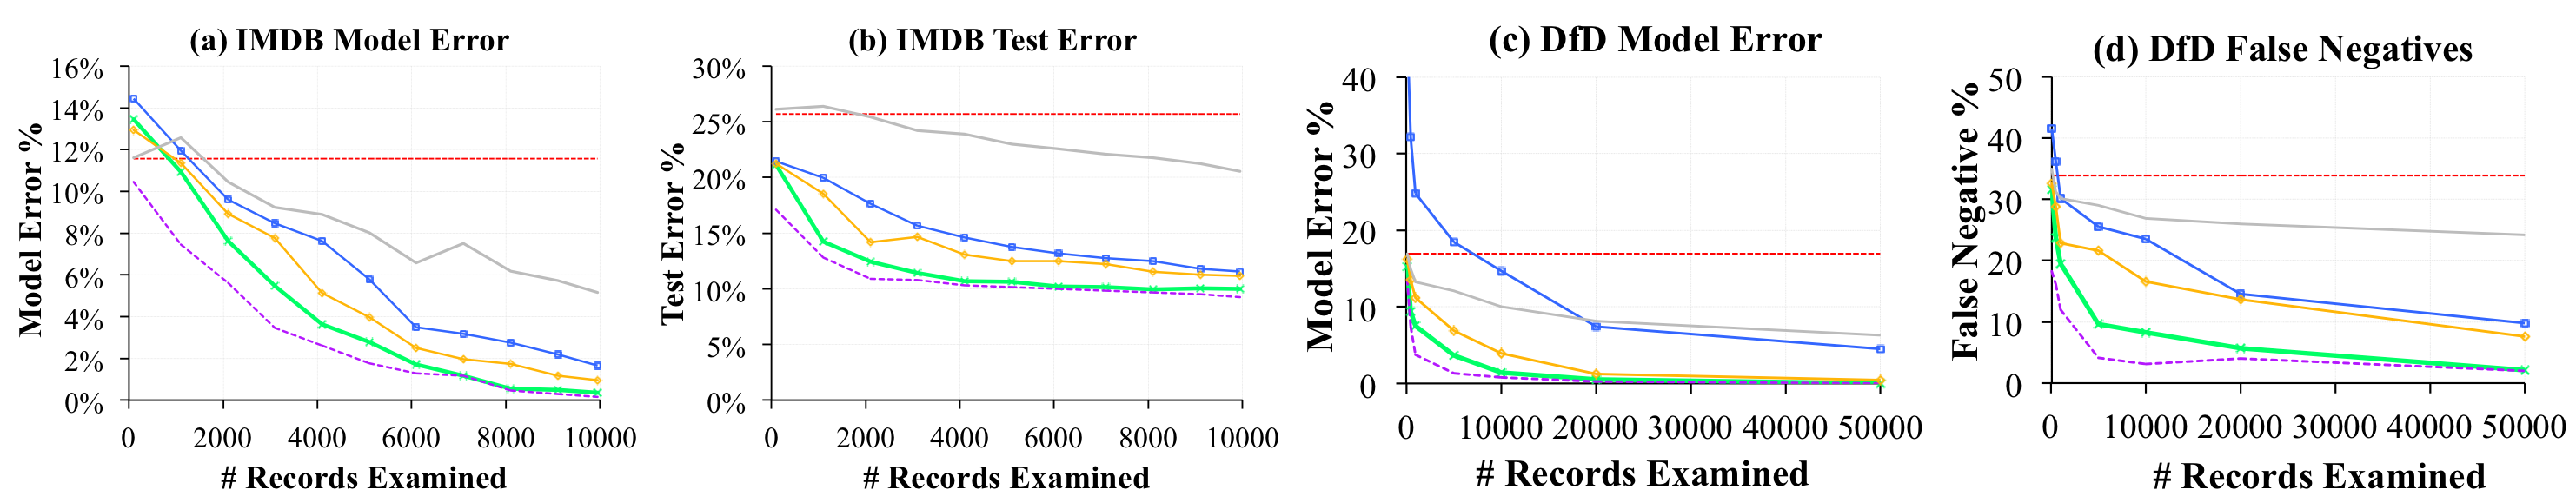
\includegraphics[width=\textwidth]{exp/real-experiments-full.png}
 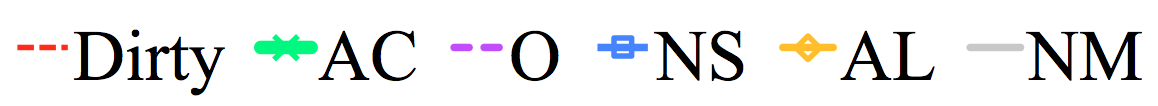
\includegraphics[width=0.6\columnwidth]{exp/legend-real.png}
 \caption{(a) We plot the relative model error as a function of the number of records cleaned for each of the alternatives on the IMDB content tagging task. \sys results in the fastest convergence. (b) Faster convergence translates into improved test accuracy. On a holdout set of 20\%, \sys is more accurate than the alternatives. (c) We evaluate \sys on the Dollars For Docs fraud detection task and find similar results, where \sys converges faster than the alternatives. (d) \sys improves the false negative rate (detection error) of the classifier resulting in an improved fraud detector. \label{real}}
\end{figure*}

\subsection{Real Scenarios}\label{real-errors}
We now describe two data analyst classification scenarios based on popular industry use cases reported in the Apache Spark user survey~\cite{sparksurvey} --- these experiments are run with real data and real corruption.
The first is a content tagging problem to categorize movies from plot descriptions; 
the second is a fraud detection problem to  determine whether a medical donation is suspicious.
Both of the datasets are plagued by systematic errors that affect the classification accuracy by $10-35\%$.
One indication of the systematic nature of the data error is that errors disproportionately affect one class rather than another.
We simulate the analyst's cleaning procedure by looking up the cleaned value in the dataset that we cleaned beforehand.
See~\cite{activecleanarxiv} for constraints, errors, and cleaning methodology, as well as an additional regression scenario.

%\reminder{Can I propose using "Records Examined" as the x-axes instead of "records cleaned"?}

\subsubsection{Movie Prediction}\label{imdb}
The first scenario uses two published datasets about movies, from IMDB~\footnote{\tiny \url{ftp://ftp.fu-berlin.de/pub/misc/movies/database/}} and Yahoo~\footnote{\tiny \url{http://webscope.sandbox.yahoo.com/catalog.php?datatype=r}}.
Each movie has a title, a short 1-2 paragraph plot description, and a list of categories, and the goal is to train a model to predict whether a movie is a ``Horror'' or ``Comedy'' from the description and title.  
The text data was featurized using a TFIDF model.

The IMDB dataset has 486,298 movies and is very dirty.  
The category list of many movies has redundant and possibly conflicting tags (e.g., ``Kids'' and ``Horror'' for the same movie).   
Also, the plot and title text may have errors from the scraping procedure (e.g., ``br\^Cuin, the'').
This dataset also shows experimental evidence for systematic bias.
Horror movies were more likely to be erroneously tagged, and consequently, a classifier trained on the dirty data favored ``Comedy'' predictions.
In contrast, the smaller Yahoo dataset (106,959 movies) is much cleaner, and nearly all of the movies are found in the IMDB dataset.

To clean the category lists, this smaller dataset to cross-referencing records when possible and import categories from Yahoo.
This was done using a simple entity resolution to match movie titles between the two dataset.
When there was a sufficiently close textual match (in terms of title string similarity), we imported the Yahoo dataset's category list to the IMDB dataset.
For the movies that did not match, we appended the records to the IMDB dataset.
Finally, we filtered the dataset for movies whose category lists included ``Horror'' or ``Comedy''.
To clean the parsing errors, we identify common parsing artifacts in each sampled batch and write a script to fix all records with that problem (e.g., remove all instances of ``\^C'').




% The first scenario explores a dataset of movie descriptions scrapped from the Internet Movie Database (IMDB)\footnote{\url{ftp://ftp.fu-berlin.de/pub/misc/movies/database/}}. 
% Each movie has a title, a 1-2 paragraph plot description, and a list of categories.
% We want to train a model that predicts whether a movie is a ``Horror'' movie or a ``Comedy'' from the plot description and the title.
% These textual attributes are featurized using a TFIDF model and stop words are removed. 
% 
% However, since much of this data is user contributed, the category list of the movies is often very dirty with redundant and sometimes conflicting tags (e.g., ``Kids and Family'' and ``Horror''). 
% Furthermore, the dataset was scrapped in HTML and then encoded in Markdown leaving a number of artifacts of parsing in the plot descriptions (e.g., ``results fr\^Celf, the'').
% Fortunately, we were able to find a much smaller but cleaner dataset from Yahoo of 106959 movies, almost all of which were contained in the IMDB dataset.
% Using this cleaner reference dataset, we matched titles and imported categories when possible.
% We also appended the cleaner plot descriptions from Yahoo to the IMDB descriptions when available.
% The clean dataset had about 10\% less examples than the dirty dataset since some movies were marked as neither  ``Horror'' or ``Comedy''.

Figure \ref{real}a plots the model error and test error versus the number of records examined by each algorithm. 
For very small batches of data (e.g., 50 out of 400,000), some of the techniques are actually less accurate than the dirty model. 
This is because the error due to the particular initial sampled batch of dominates, and we find that differences between the techniques are not statistically significant in that regime.
However, as more data is cleaned, we see a clear seperation between the techniques
%as more records are cleaned. 
The purple bottom curve is the Oracle approach, and we find that out of the practical approaches \sys reduces the model error the fastest, and is the only method that converges to the Oracle performance.
Figure~\ref{real}b directly shows how \sys rapidly reduces the test error --- after 2000 records, \sys's test error is within 0.02 of the fully cleaned model.
\sys provides superior convergence for two main reasons.
First, the update algorithm can incorporate both the raw data as well as the smaller set of cleaned records.
This makes \sys less sensitive to sampling error.
Next, \sys also selects records that are more likely to by dirty (Section \ref{det}) and will will most improve the model (Section \ref{dist-samp}).
This is illustrated in \sys's faster convergence curve in the first 2000 cleaned records.

% We find that \sys converges faster than those trained with the alternatives.
% The reasons for this include: (1) \sys samples more data that is likely to be dirty, and (2) \sys selects data that is most valuable to the model.
% This improvement in model convergence translates into large improvements in the accuracy of the model on a holdout set Figure \ref{real}b.
% Figure \ref{real}b illustrates two points: dirty data significantly affects the quality of the model (25\% misclassification rate) and a relatively small amount of data cleaning can greatly improve the quality of the model with the appropriate update techniques.
% For 2000 records cleaned, \sys is within 2\% of the accuracy of the model if the data were fully cleaned.
% On the other hand, for the same amount of cleaning, the ``Re-training'' approach hasn't improved the model. 

% One of the reasons for this positive result is the significant systematic bias in the errors. Horror movies were more likely to be erroneously tagged. 
% On the dirty dataset, the prediction precision of the model for Horror movies was only 29\%.
% This improved to 74\% after data cleaning.

\vspace{1em}
\subsubsection{Dollars For Docs (DfD)}\label{exp:dfd}
The second scenario explores ProPublica's Dollars for Docs dataset described in Section~\ref{s:usecase}.
We featurize the 5 text attributes using a bag-of-words representation, and our goal is to predict the status of medical donations using an SVM (``allowed'' or ``disallowed'').
Figure~\ref{real}c plots the model error as a function of the number of records examined for each of the techniques.
As in the IMDB dataset, we find that \sys converges faster than Naive-Mix, Naive-Sampling, and Active Learning.
In fact, \sys can achieve comparable model accuracy (< 1\% of the true model accuracy) while expending a fraction of the data cleaning effort (10\% of the records cleaned).

In terms of test error, Figure~\ref{real}d reports the detection error or false negative \% (percentage of disallowed research contributions that the model misses) on a held-out evaluation set. 
This measures the real-world utility of the classifier learned with \sys.
The dirty and fully cleaned models have respectively a 34\% and 3\% detection error.
Due to the systematic bias in the data errors (explained in Section \ref{s:usecase}), \sys is able to identify the dirty records and
reduce the detection error to 8\% after examining 10,000 records.

Overall, we found that systematic errors are indeed present in real-world datasets, and that \sys can effectively identify and exploit this bias
to more quickly converge to the true clean model as compared to the naive or active learning approaches.  
In fact, we found that the commonly used retraining approach (Naive-Mix) was almost completely ineffective as compared to other model update techniques.

% The dataset has 240,089 records with 5 textual attributes and one numerical attribute.
% The dataset is featurized with bag-of-words featurization model for the textual attributes which resulted in a 2021 dimensional feature vector, and a binary SVM is used to classify the status of the medical donations.
% Figure \ref{real}c shows that \sys converges faster than Active Learning and SampleClean.
% To achieve a 4\% relative error (i.e., a 75\% error reduction from the dirty model), \sys cleans 40000 fewer records than Active Learning.
% Also, for 10000 records cleaned, \sys has nearly an order of magnitude smaller error than SampleClean.

% Figure \ref{real}d shows the detection rate (fraction of disallowed research contributions identified) of the classifier as a function of the number of records cleaned. 
% On the dirty data, we can only correctly classify 66\% of the suspected examples (88\% overall accuracy due to a class imbalance).
% On the cleaned data, this classifier is nearly perfect with a 97\% true positive rate (98\% overall accuracy).
% \sys converges to the cleaned accuracy faster than the alternatives with a classifier of 92\% true positive rate for only 10000 records cleaned.
% These numbers also indicate the significant systematic bias where positive examples are more likely to be corrupted.

% In short, these two scenarios illustrate the value of \sys on real datasets both of which contain significant systematic biases.
% \sys demonstrates increased accuracy for the same amount of records cleaned compared the alternatives.
% Across all of our experimental datasets, we found that the retraining approach gave poor results in addition to the correctness problems discussed in the introduction.
% For this reason, in future comparisons, we exclude retraining but discuss this in Section \ref{exp:rtr}.

\begin{figure}[t]
\centering
 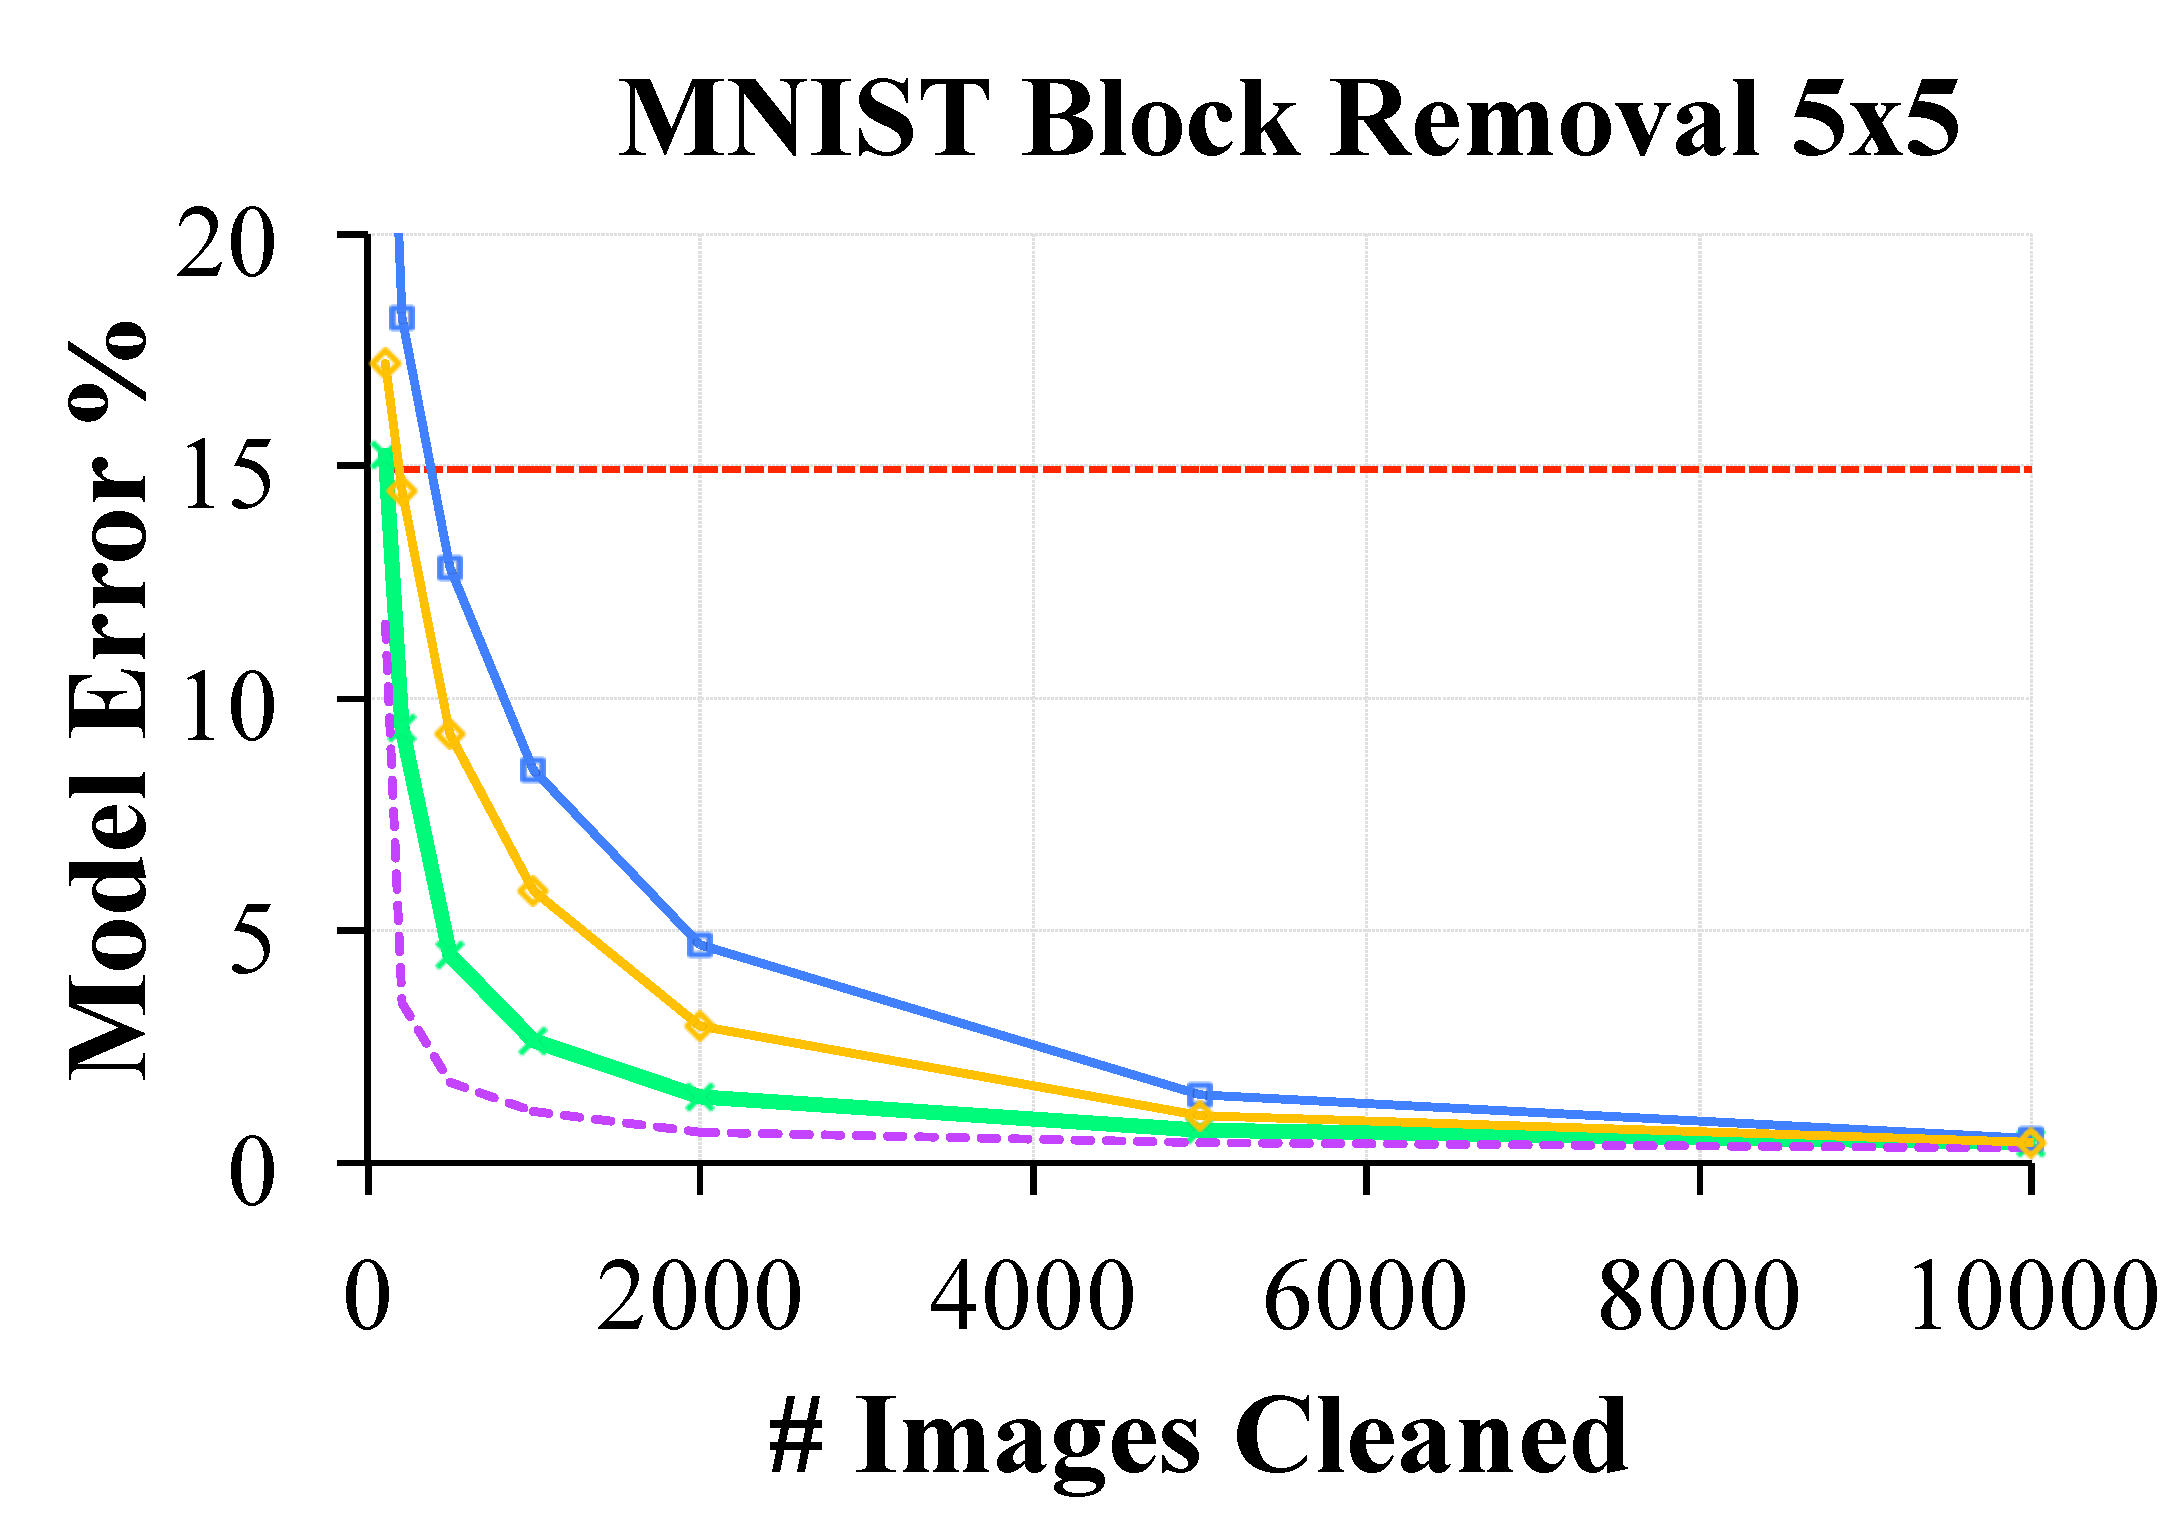
\includegraphics[width=0.49\columnwidth]{exp/exp7a.pdf}
 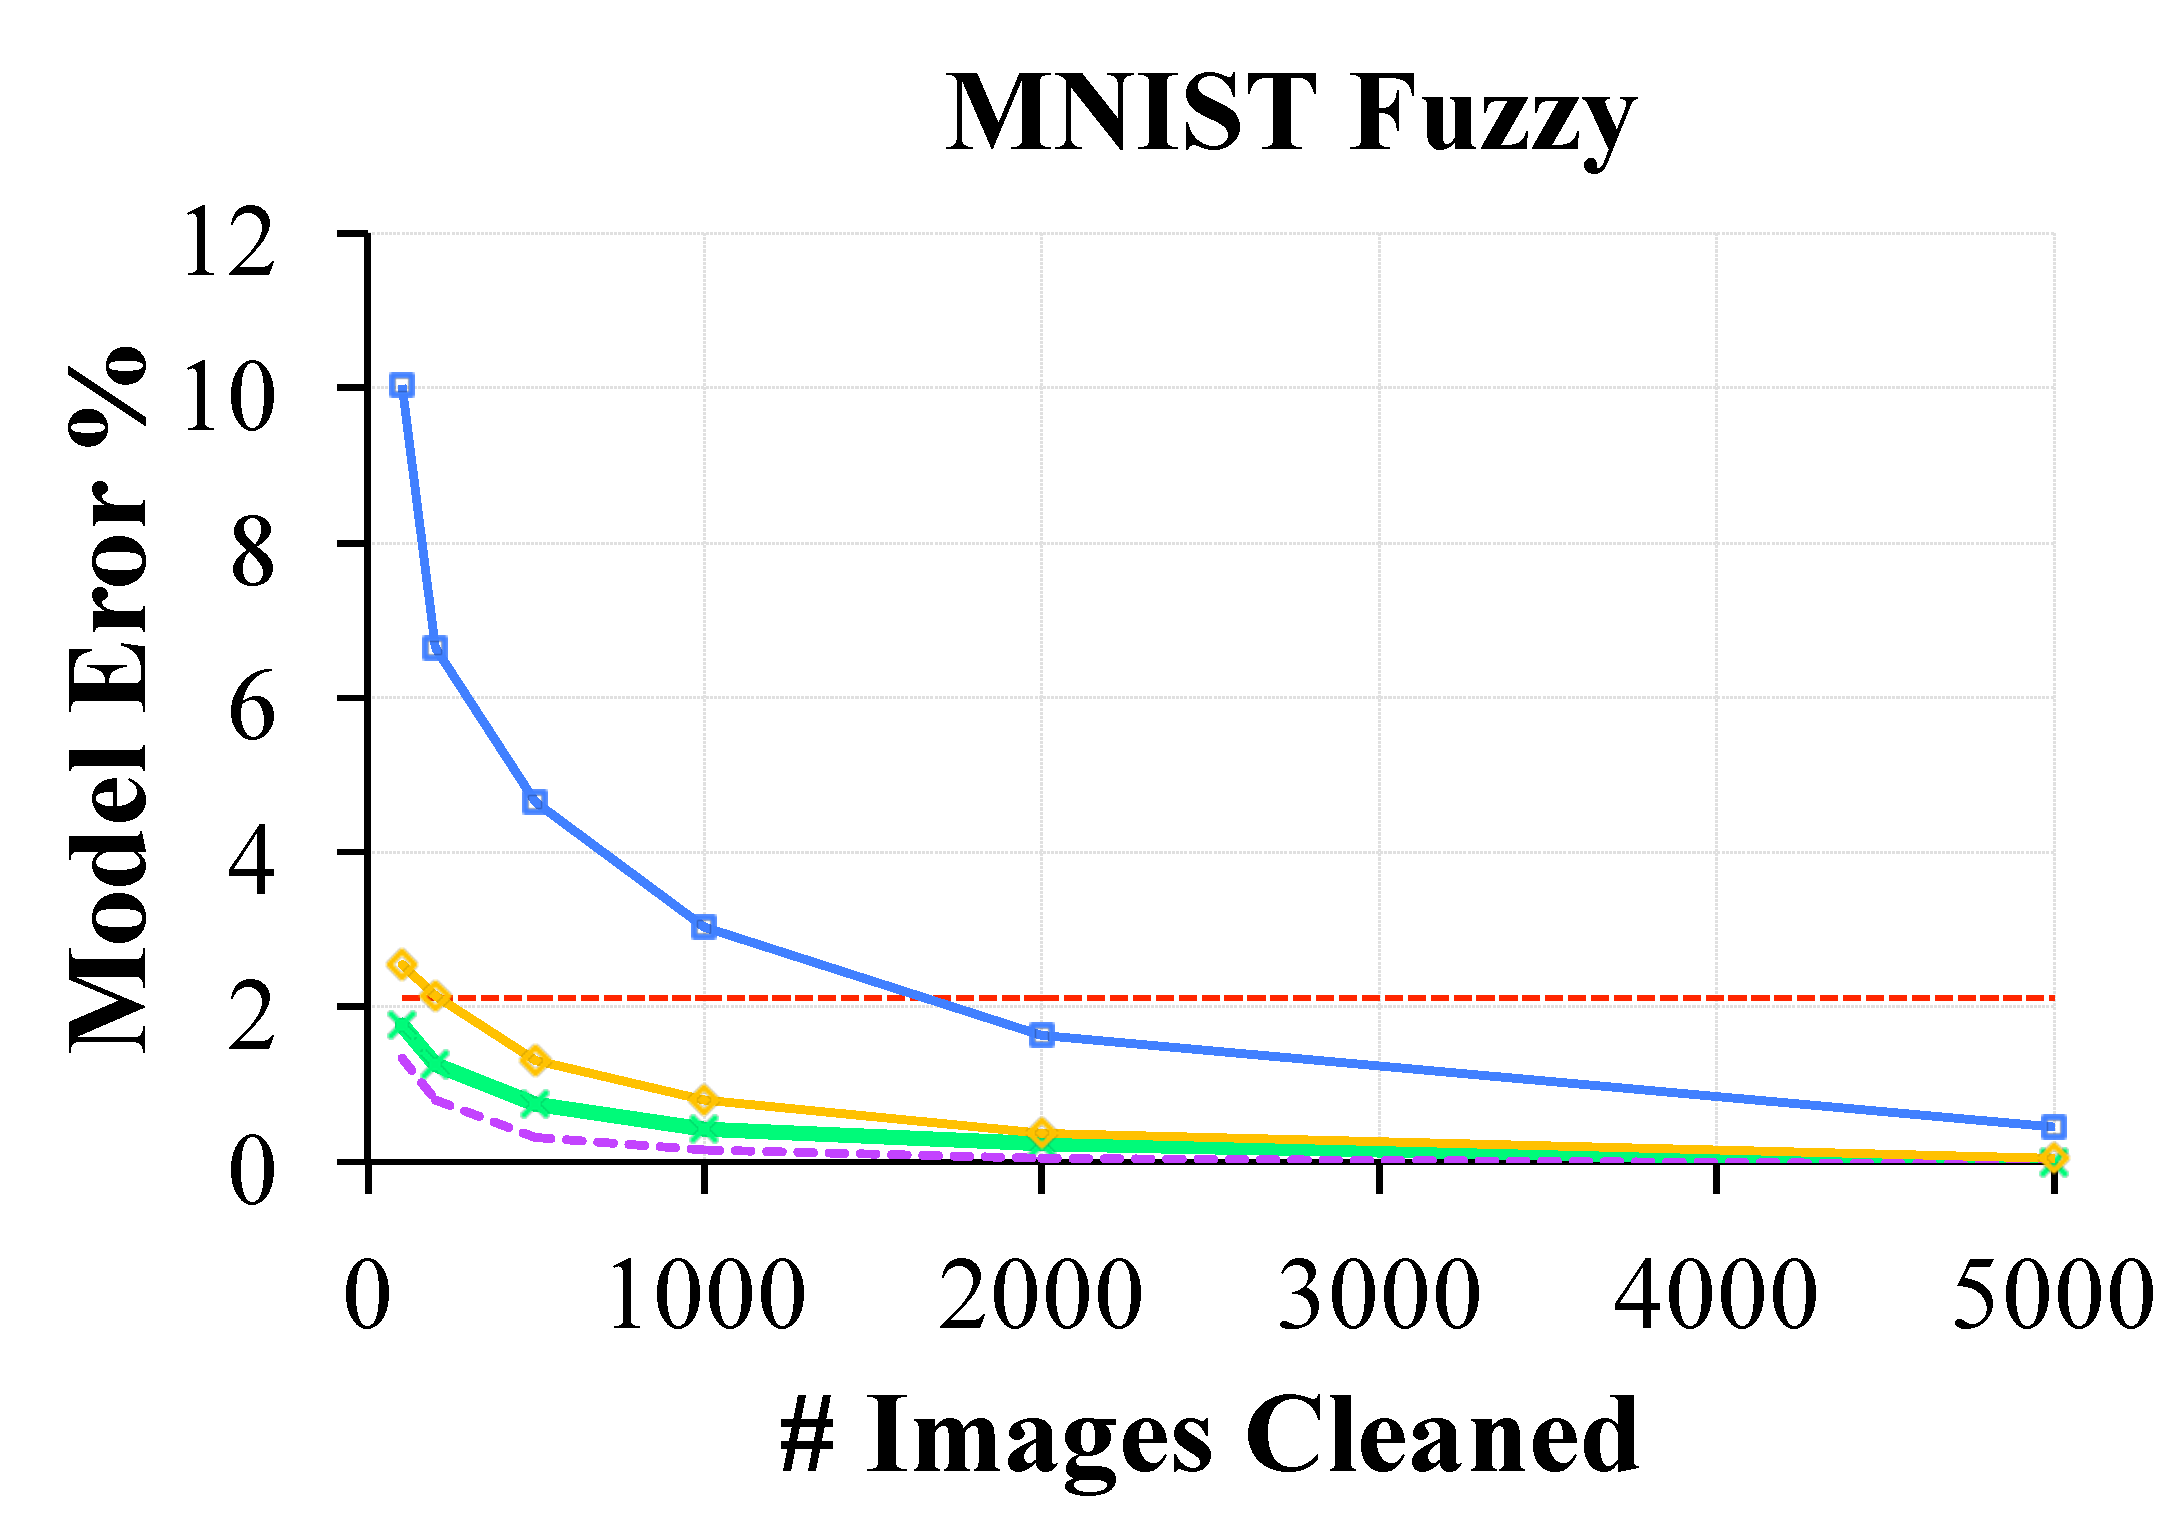
\includegraphics[width=0.49\columnwidth]{exp/exp7b.pdf}
 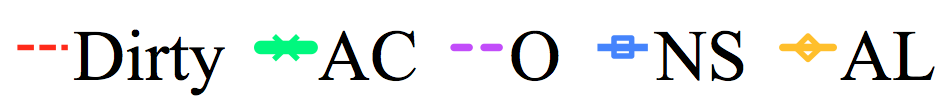
\includegraphics[width=0.49\columnwidth]{exp/legend-general.png}
 \caption{In an image processing pipeline on the MNIST dataset with simulated errors, \sys outperforms Active Learning and Naive-Sample.  \label{mnist}}
\end{figure}

\vspace{4em}
\subsection{Simulated Machine Learning Pipeline}
This experiment is representative of modern machine learning pipelines such as AMPLab's Keystone ML~\cite{keystone} and Google's Tensor Flow~\cite{tensor}. 
The task is to classify 60,000 images of handwritten digits from the MNIST dataset into 10 categories with a one-to-all multiclass SVM classifier~\footnote{\scriptsize\url{http://ufldl.stanford.edu/wiki/index.php/Using_the_MNIST_Dataset}}. 
In contrast to the prior scenarios, which directly extracted feature vectors from the raw dataset, image feature extraction involves a pipeline of transformation steps including edge detection, projection, and raw image patch extraction~\cite{keystone,tensor}.
The cleaning function $C()$ involves replacing a potentially corrupted image with a non-corrupted version.
We find that pipelines tend to propagate small amounts of corruption, and in fact, and even randomly generated errors can morph into systematic biases.
% What is unique about image processing is that data are often processed through a pipeline of operators edge detectors, projections, and raw image patches~\cite{keystone,tensor}.
% This experiment explores data cleaning in this context, where dirtiness is in the raw data but get propagated through the pipeline.

% We use the MNIST handwritten digit recognition dataset with a MATLAB image processing pipeline.
% In this scenario, the analyst must inspect a potentially corrupted image and replace it with a higher quality one.
% The MNIST dataset consists of 64x64 grayscale images.
There are two types of simulated corruptions that mimic standard corruptions in image processing (occlusion and low-resolution): \texttt{5x5 Removal} deletes a random 5x5 pixel block by setting the pixel values to 0, and \texttt{Fuzzy} blurs the entire image using a 4x4 moving average patch. 
We apply these corruptions to a random 5\% of the images.

Figure \ref{mnist} shows that \sys makes more progress towards the clean model with a smaller number of examples cleaned.
To achieve a 2\% error for 5x5 Removal, \sys can inspect 2200 fewer images than Active Learning and 2750 fewer images than Naive-Sampling.
For the fuzzy images, both Active Learning and \sys reach 2\% error after examining $<100$ images, while Naive-Sampling requires 1750.
Even though these corruptions are generated independently of the data, the \texttt{5x5 Removal} propagates through the pipeline as a systematic error.
The image features are constructed with edge detectors, which are highly sensitive to this type of corruption.
Digits that naturally have fewer edges than others are disproportionately affected since the removal process adds spurious edges.
On the other hand, the \texttt{Fuzzy} corruption propagates through the pipeline are similar to random errors (as opposed to systematic).
%This experiment highlights that featurization and other data processing pipelines between the raw data and model can introduce systematic biases in the presence of data corruption.

\subsection{Simulated Error Scenarios}
In the next set of experiments, we use standard Machine Learning benchmark datasets and corrupt them with varying levels of systematic noise.
We use this to evaluate \sys while isolating certain variables.
The two datasets that we used were:

\vspace{0.25em}

\noindent\textbf{Income Classification (Adult): } In this dataset of 45,552 records, the task is to predict the income bracket (binary) from 12 numerical and categorical covariates with an SVM classifier. 

\vspace{0.25em}

\noindent\textbf{Seizure Classification (EEG): } In this dataset, the task is to predict the onset of a seizure (binary) from 15 numerical covariates with a thresholded Linear Regression. There are 14980 data points in this dataset. This classification task is inherently hard with an accuracy on the completely clean data of only 65\%.

\begin{figure}[t]
\centering
 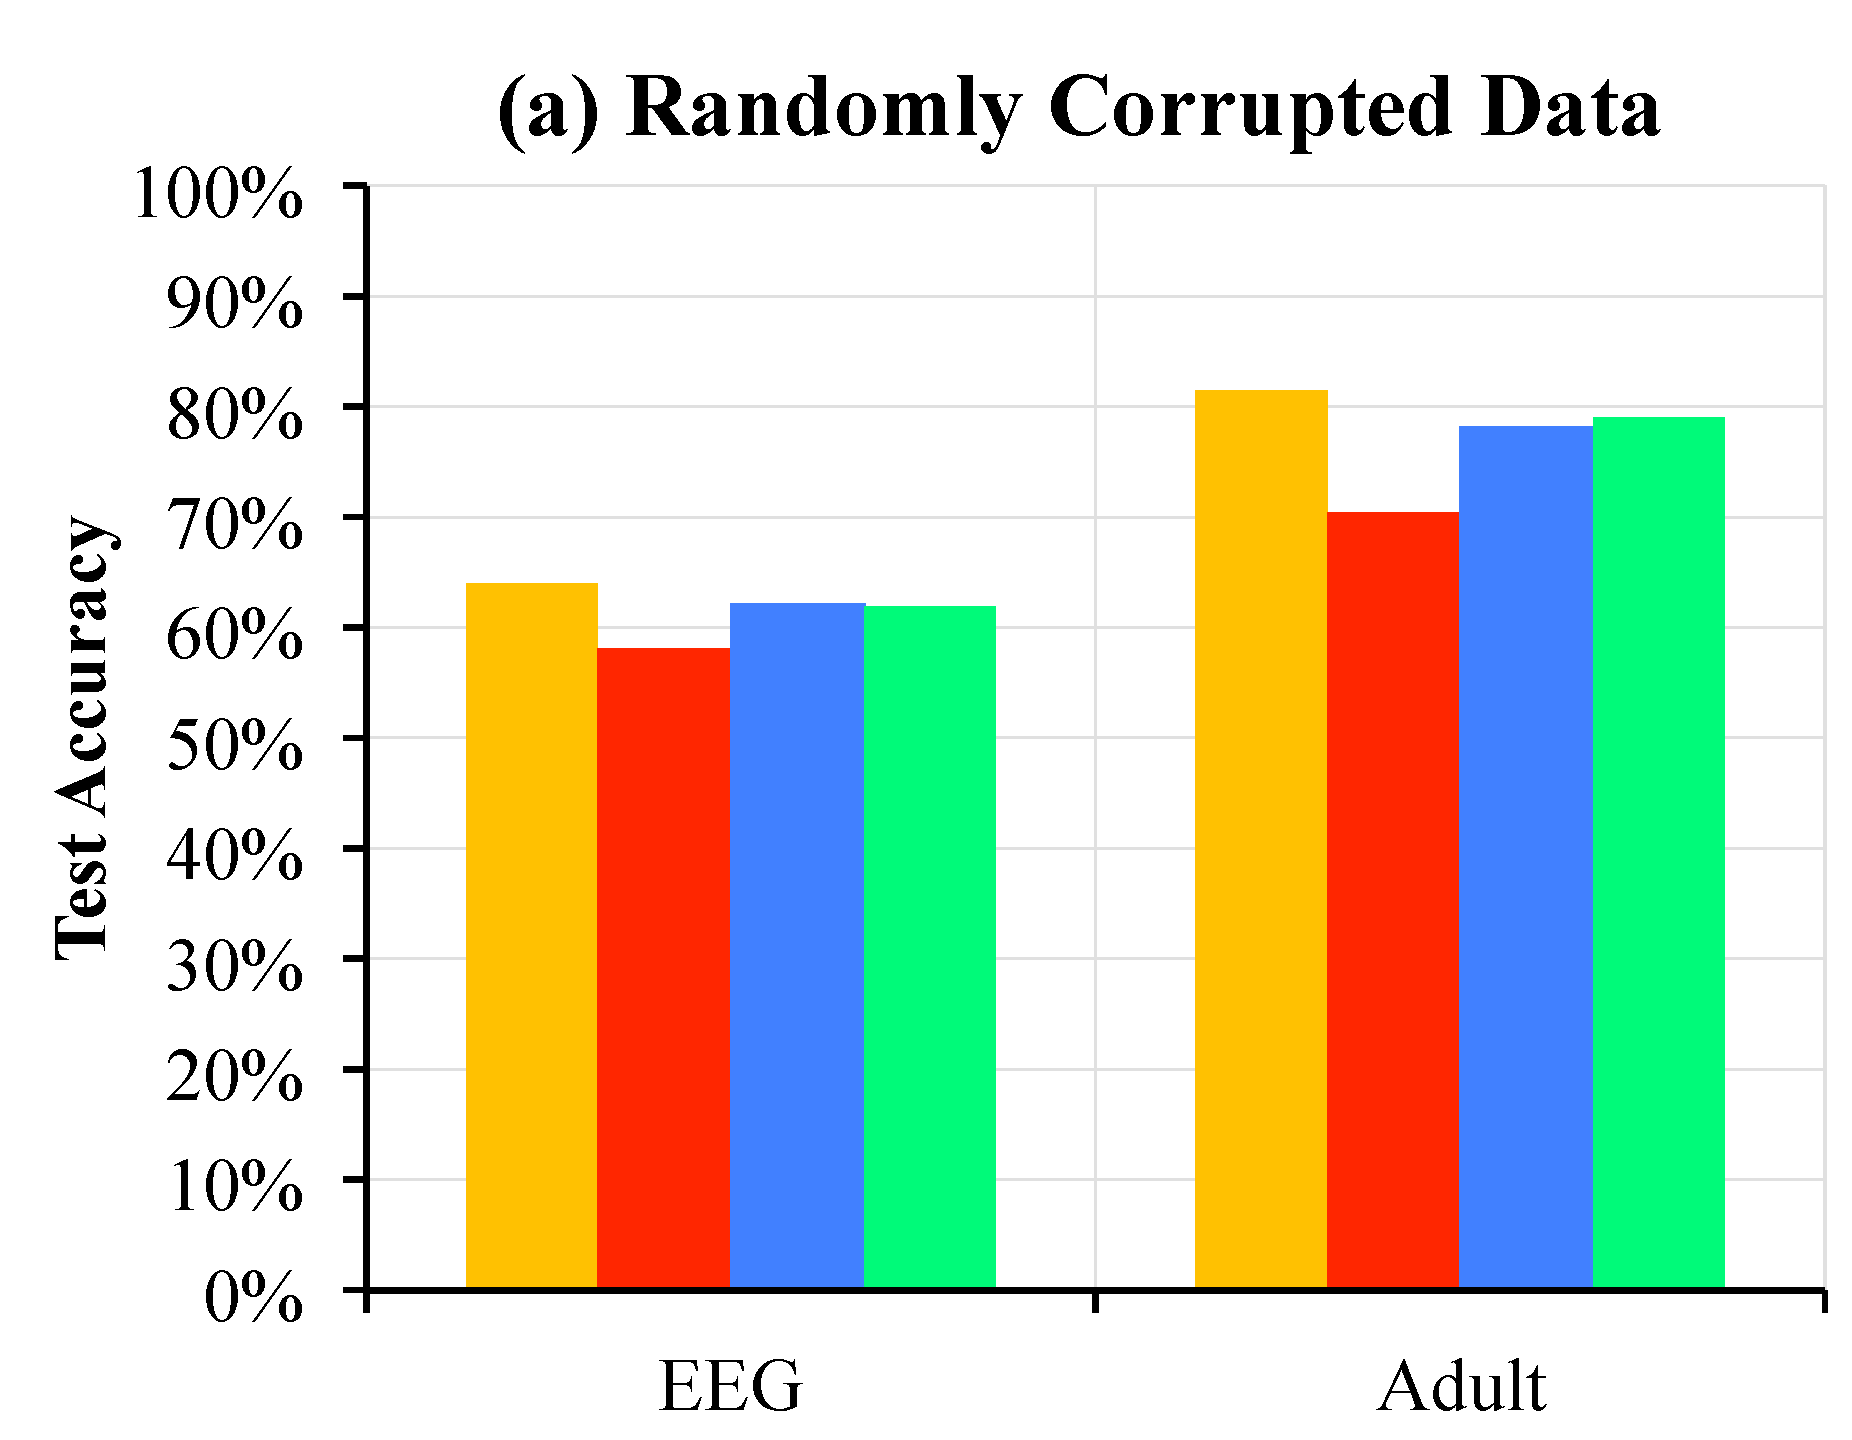
\includegraphics[width=0.49\columnwidth]{exp/exp2.pdf}
 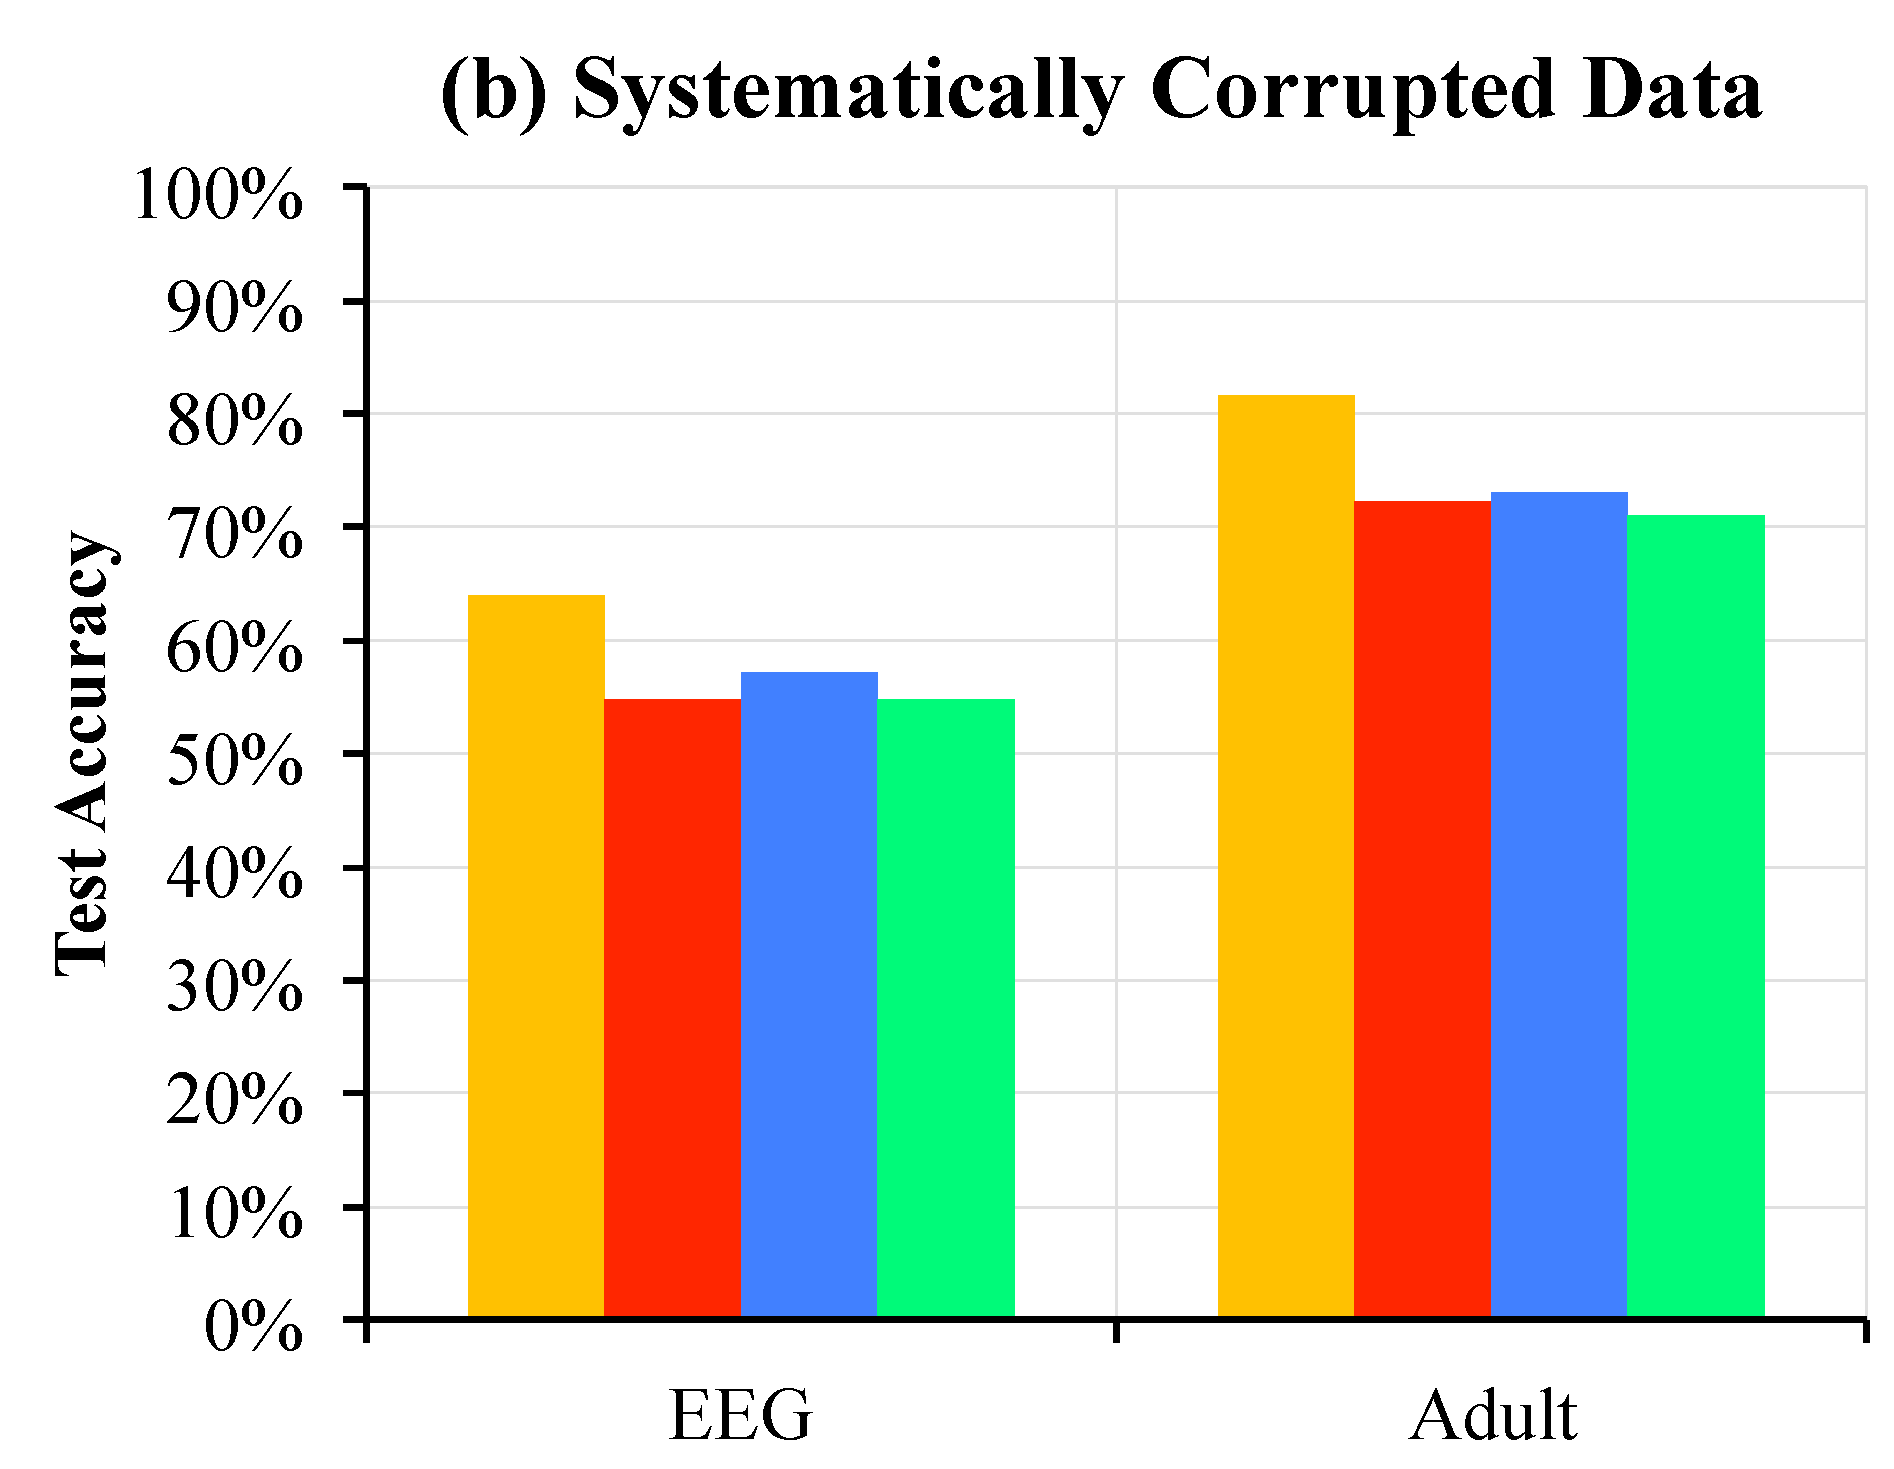
\includegraphics[width=0.49\columnwidth]{exp/exp1.pdf}
 
\includegraphics[width=0.5\columnwidth]{exp/legend-1.png}
 \caption{(a) Robust techniques and discarding data work when corrupted data are random and look atypical. (b) Data cleaning can provide reliable performance in both the systematically corrupted setting and randomly corrupted setting.\label{sys-rand}}
\end{figure}

\subsubsection{Data Cleaning v.s. Robust Statistics}
Machine Learning has broadly studied a number of \emph{robust} methods to deal with some types of outliers. In particular, this field studies random high-magnitude outliers and techniques to make statistical model training agnostic to their presence. Feng et al. proposed a variant of logistic regression that is robust to outliers~\cite{feng2014robust}. We chose this algorithm because it is a robust extension of the convex regularized loss model, leading to a better apples-to-apples comparison between the techniques.
Our goal is to understand which types of data corruption are amenable to data cleaning and which are better suited for robust statistical techniques.
The experiment compares four schemes: (1) full data cleaning, (2) baseline of no cleaning, (3) discarding the dirty data, and (4) robust logistic regression. 
We corrupted 5\% of the training examples in each dataset in two different ways:

\vspace{1em}

\noindent\textbf{Random Corruption: } Simulated high-magnitude random outliers. 5\% of the examples are selected at random and a random feature is replaced with 3 times the highest feature value.

\vspace{0.5em}

\noindent\textbf{Systematic Corruption: } Simulated innocuous looking (but still incorrect) systematic corruption. The model is trained on the clean data, and the three most important features (highest weighted) are identified. The examples are sorted by each of these features and the top examples are corrupted with the mean value for that feature (5\% corruption in all). 
%It is important to note that examples can have multiple corrupted features.

\vspace{1em}

Figure \ref{sys-rand} shows the test accuracy for models trained on both types of data with the different techniques.
The robust method performs well on the random high-magnitude outliers with only a 2.0\% reduction in clean test accuracy for EEG and 2.5\% reduction for Adult.
In the random setting, discarding dirty data also performs relatively well.
However, the robust method falters on the systematic corruption with a 9.1\% reduction in clean test accuracy for EEG and 10.5\% reduction for Adult.
Data cleaning is the most reliable option across datasets and corruption types.
The problem is that without cleaning, there is no way to know if the corruption is random or systematic and when to trust a robust method.
While data cleaning requires more effort, it provides benefits in both settings.
The remaining experiments, unless otherwise noted, use systematic corruption.

\subsubsection{Source of Improvements}\label{comp}
This experiment compares the performance of \sys with and without various optimizations for 500 records examined. 
\sys without detection is denoted as (AC-D) (that is at each iteration we sample from the entire dirty data), and \sys without detection and our prioritized sampling is denoted as (AC-D-I).
Figure \ref{opts} plots the relative error of the alternatives and \sys with and without the optimizations.
Without detection (AC-D), \sys is still more accurate than Active Learning.
Removing the sampling, \sys is slightly worse than Active Learning on the Adult dataset but is comparable on the EEG dataset.
The advantage of \sys is that it is a composable framework supporting different instantiations of the detection and prioritization modules while still preserving convergence guarantees.
With these optimizations, \sys is consistently more efficient than Active Learning.

\begin{figure}[t]
\centering
 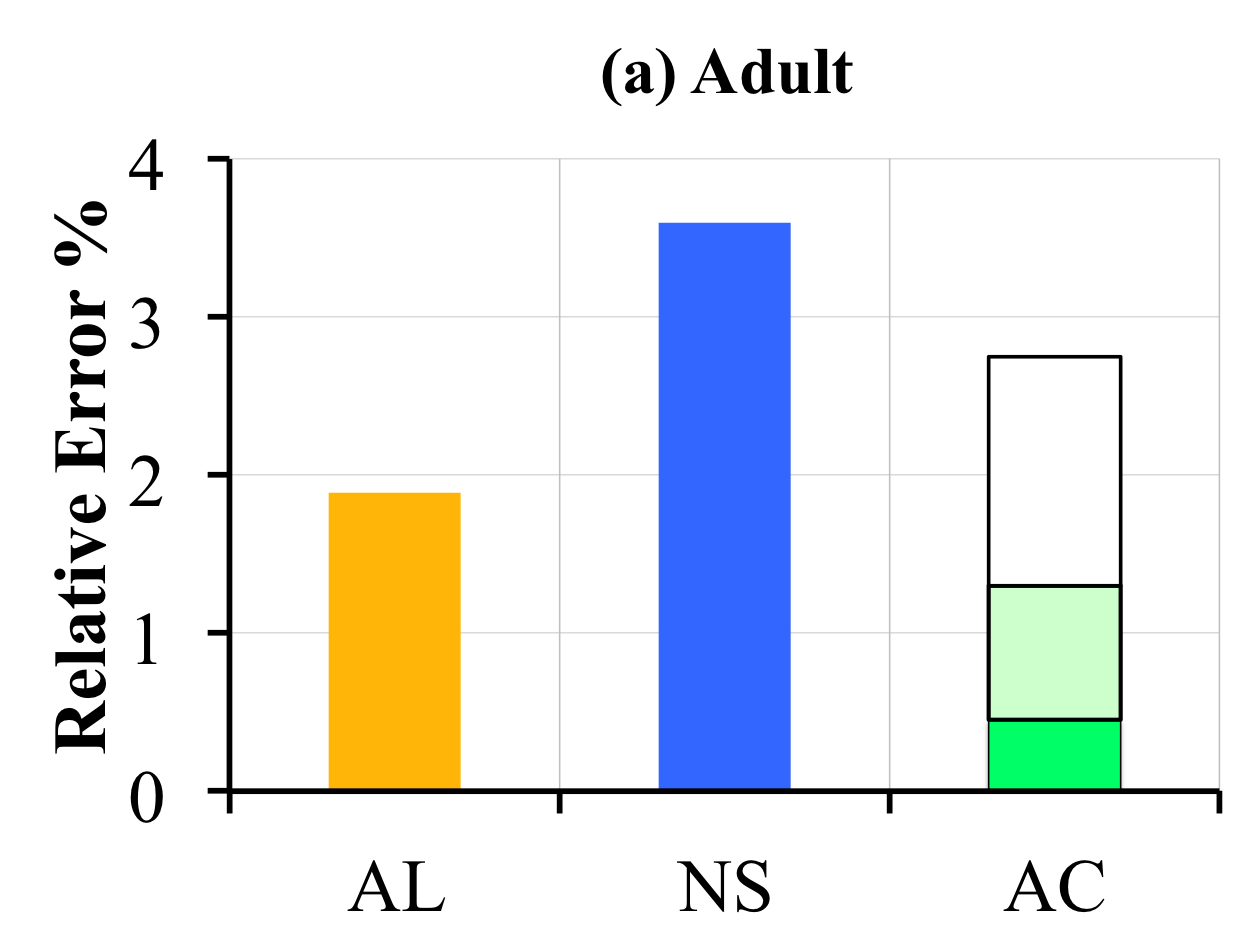
\includegraphics[width=0.49\columnwidth]{exp/exp8a.png}
 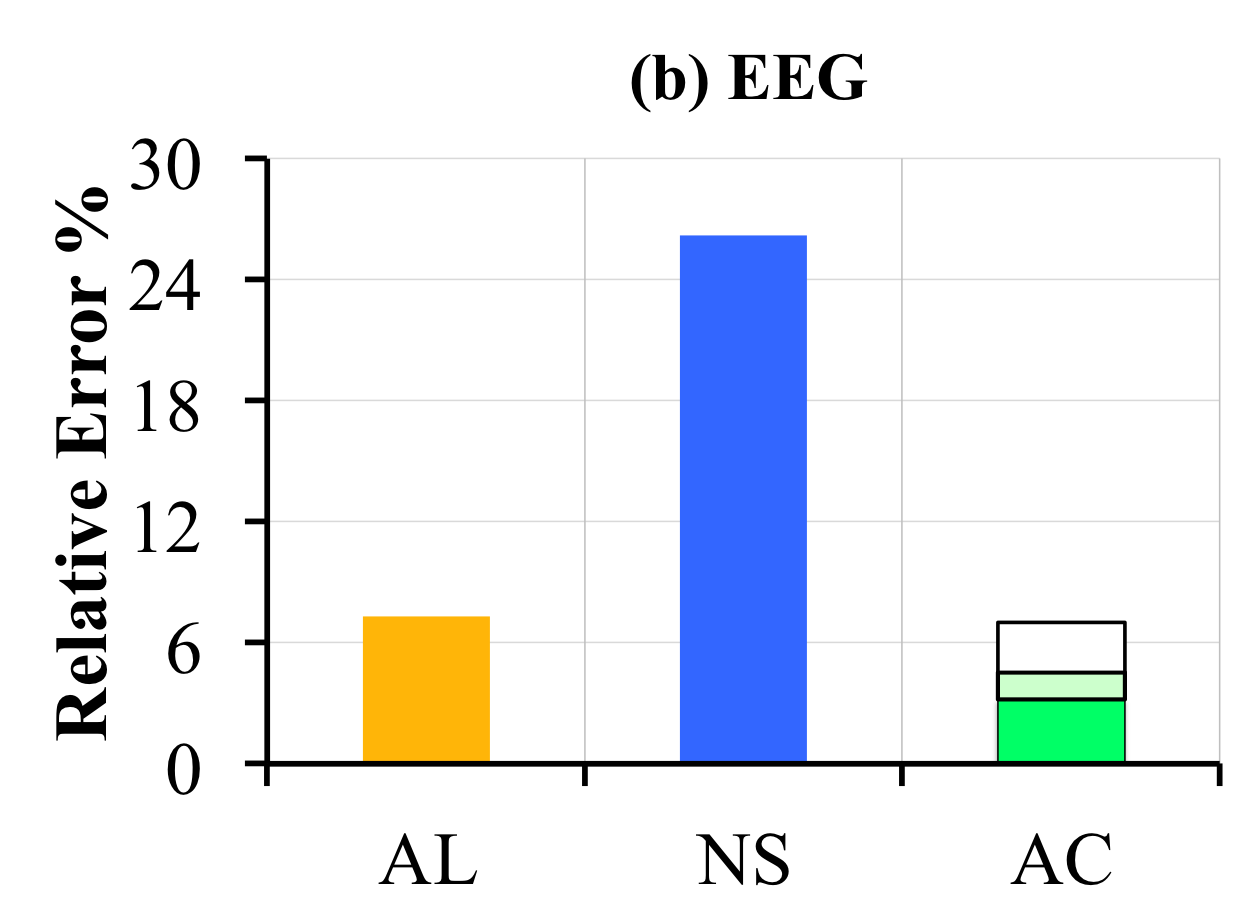
\includegraphics[width=0.49\columnwidth]{exp/exp8b.png}
 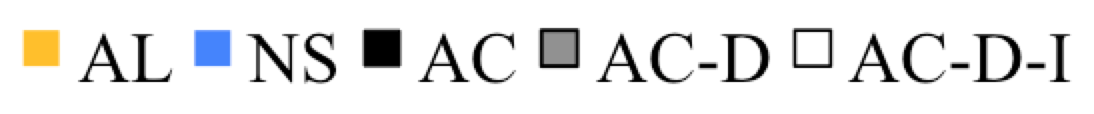
\includegraphics[width=0.5\columnwidth]{exp/legend-8.png}
 \caption{ -D denotes no detection, and -D-I denotes no detection and no importance sampling. Both optimizations significantly help \sys outperform Naive-Sampling and Active Learning. \label{opts}}
\end{figure}

\subsubsection{Mixing Dirty and Clean Data}\label{exp:rtr}
Naive-Mix is an unreliable methodology lacking the same guarantees as Active Learning or Naive-Sampling even in the simplest of cases.
We also saw that it is significantly less efficient than \sys, Naive-Sampling, and Active Learning on the real datasets.
For thoroughness, these experiments include the model error as a function of records examined in comparison to \sys.
We also evaluate this approach with our detection component.
Naive-Mix+D randomly samples data using the dirty data detector, applies the user-specified cleaning, and writes-back the cleaned data.

Figure \ref{pc-perf} plots the same curves as the previous experiment comparing \sys, Active Learning, and two mixed data algorithms.
Intuitively, Naive-Mix makes less progress with each update.
Consider the case where 10\% of the dataset is corrupted and a small sample of data 1\%.
\sys and Naive-Sampling extrapolate from the cleaned sample (\sys extrapolates a gradient) while Naive-Mix considers the entire dirty data which might be much larger.

%\sys converges faster.
%\sys tunes the weighting when averaging dirty and clean data into the gradient.

\begin{figure}[ht!]
\centering
 %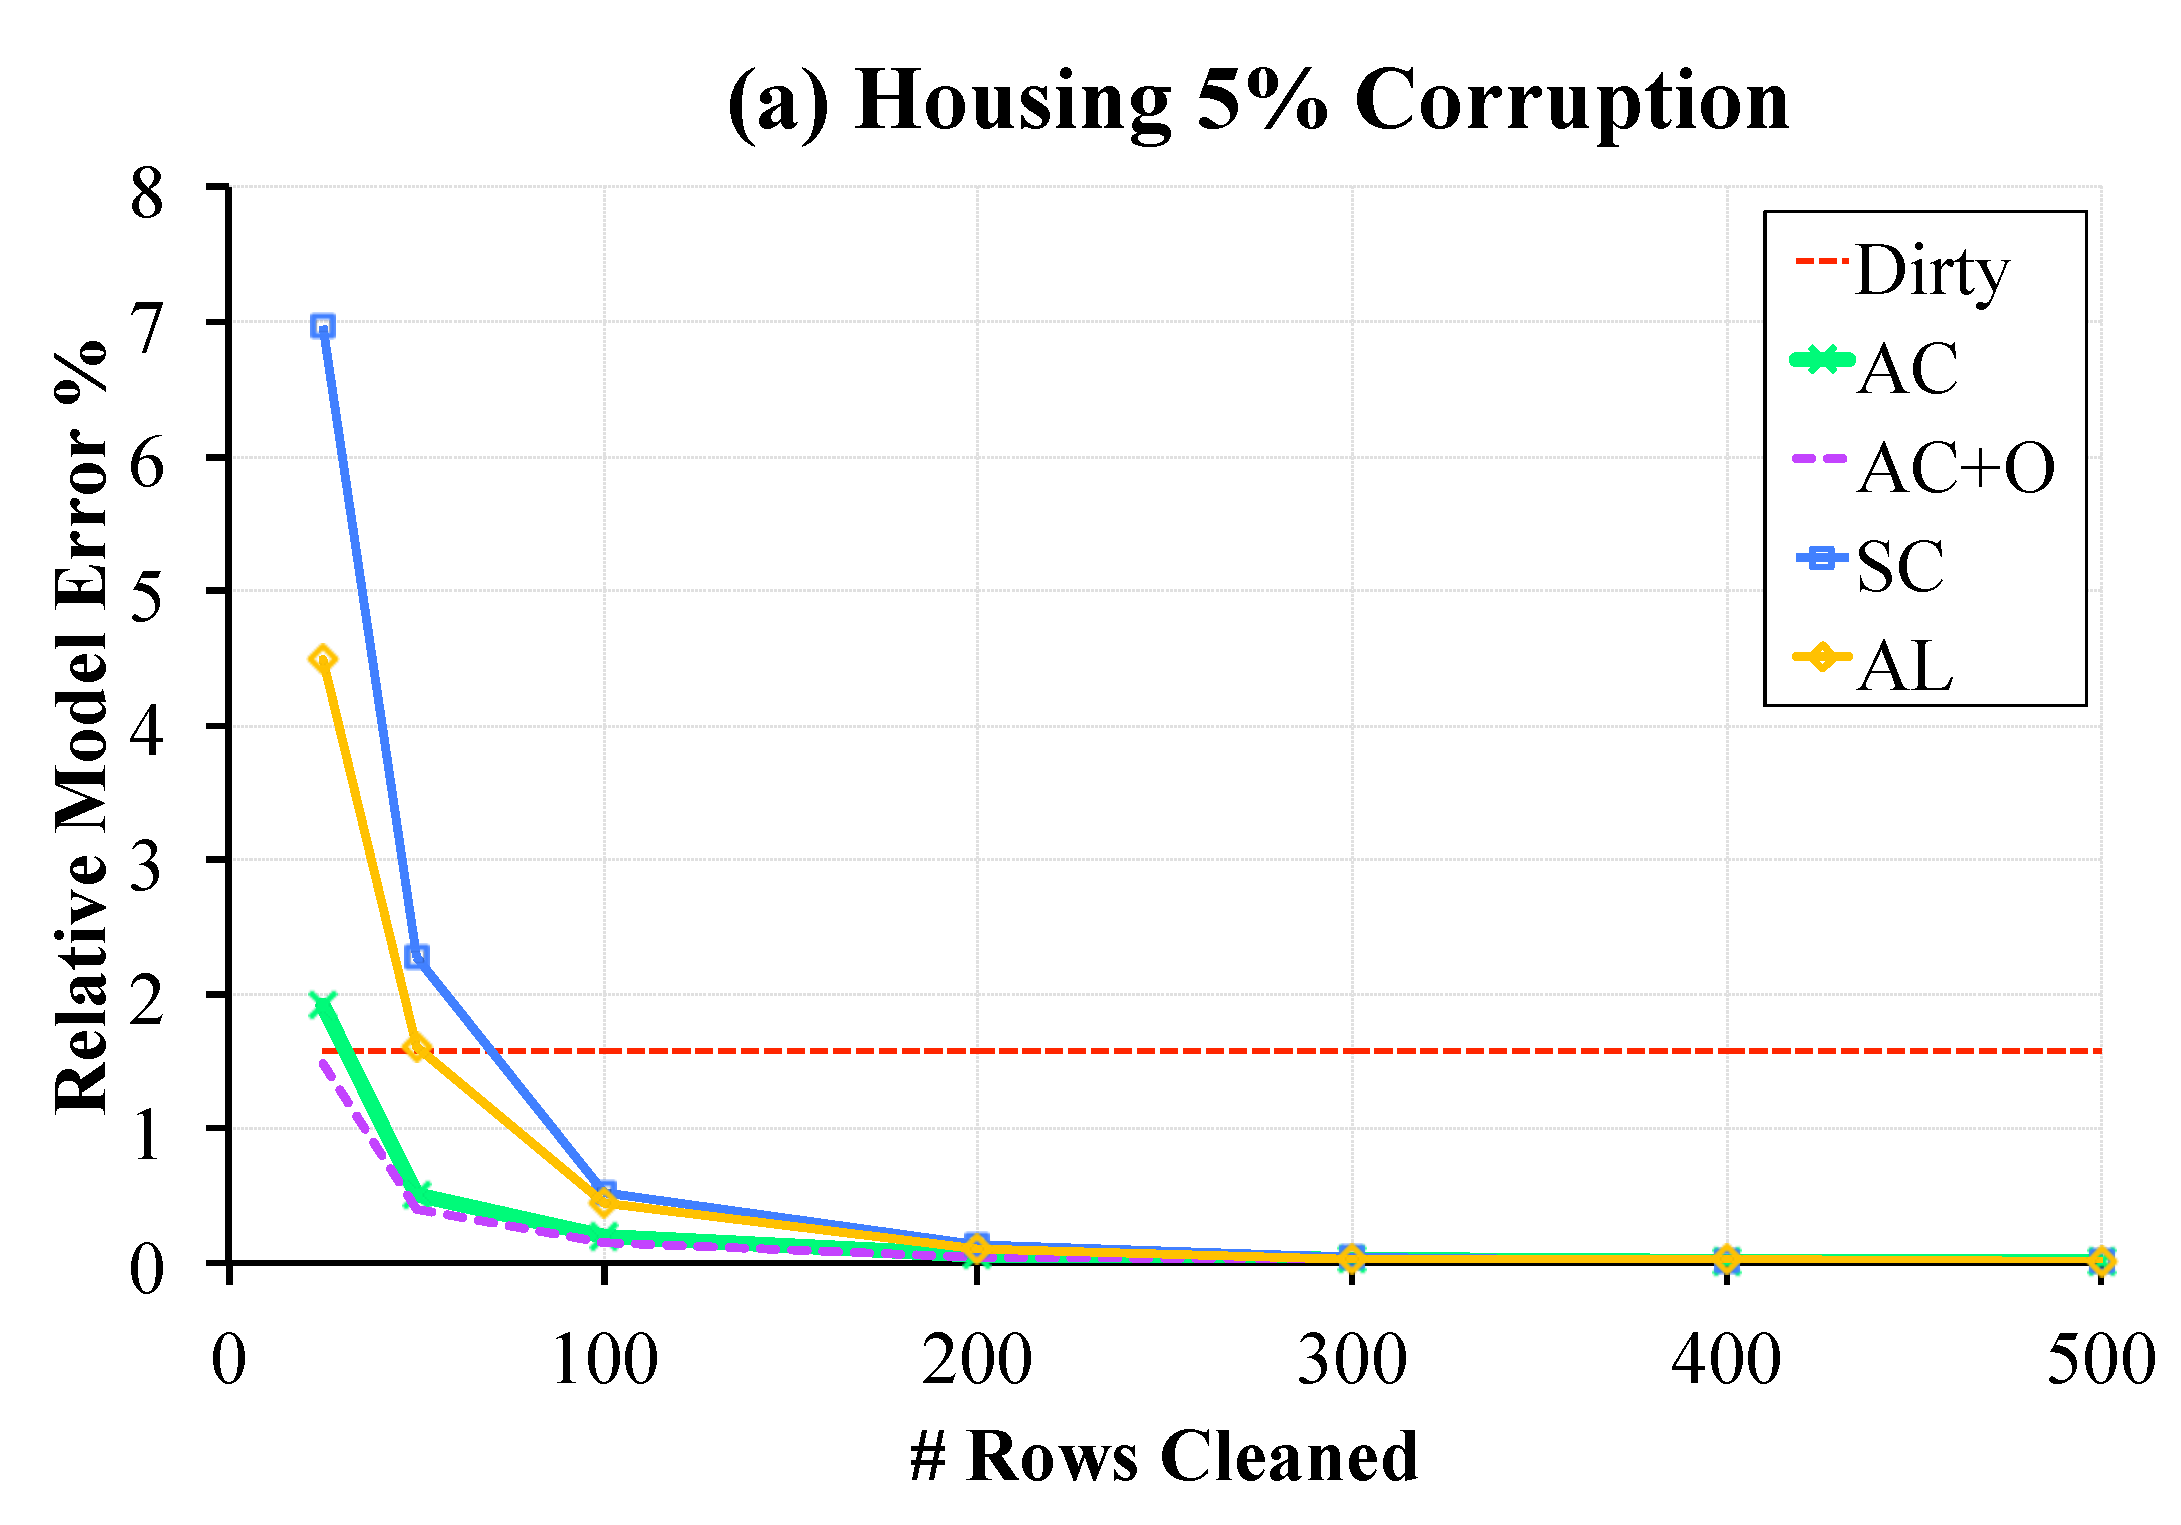
\includegraphics[scale=0.15]{exp/exp3a.pdf}
 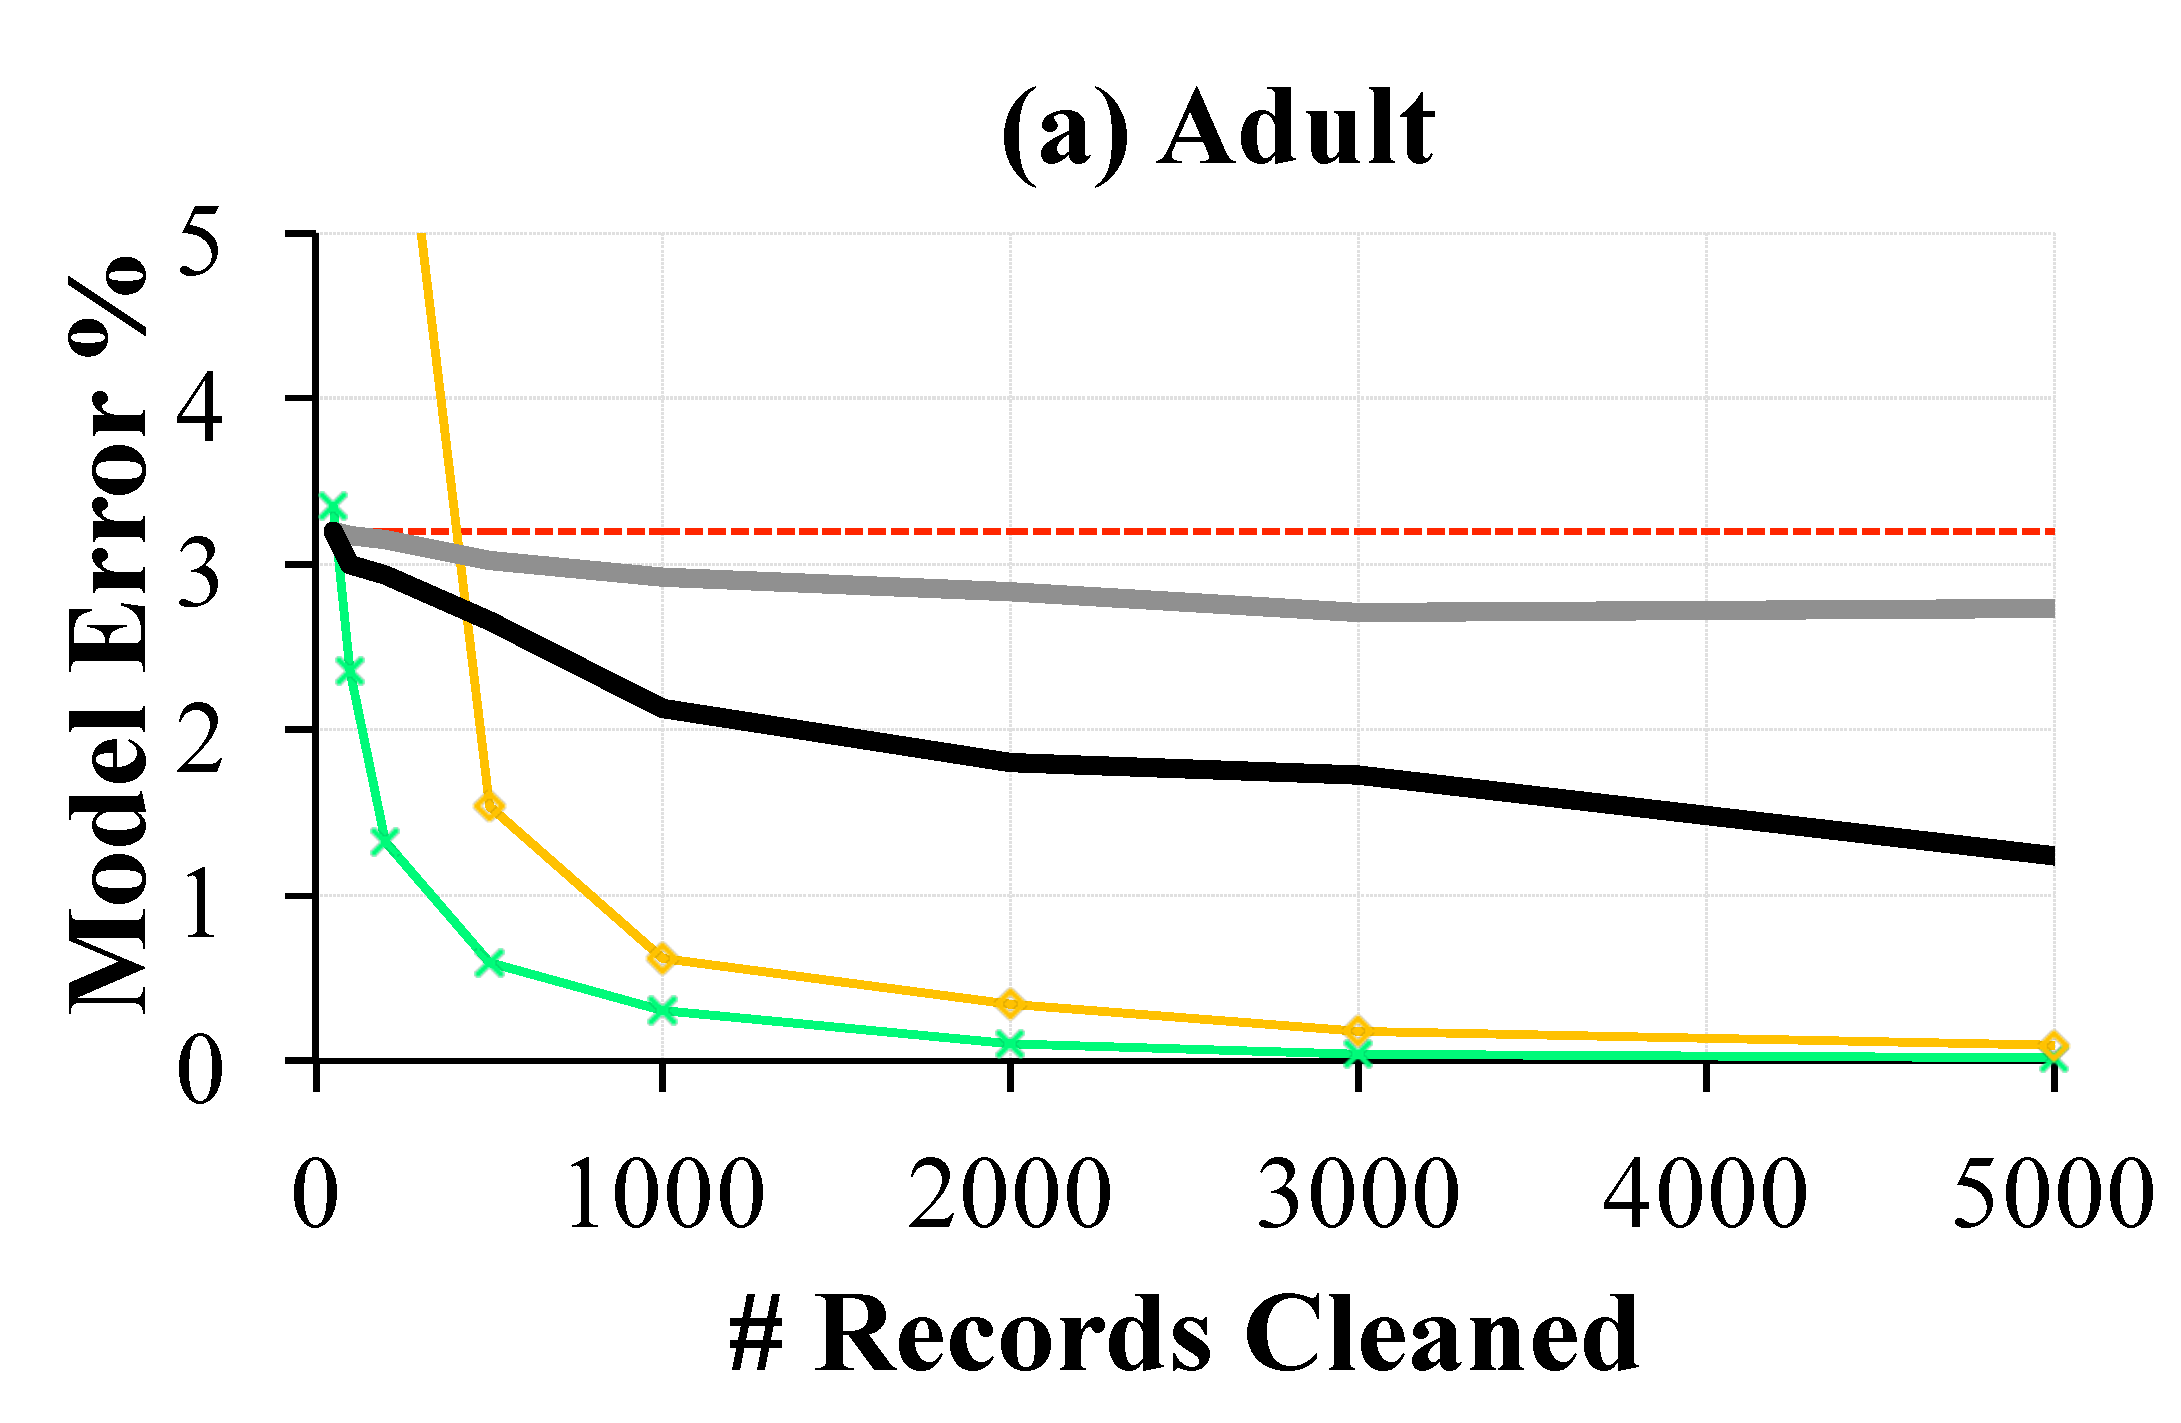
\includegraphics[width=0.49\columnwidth]{exp/exp14a.pdf}
    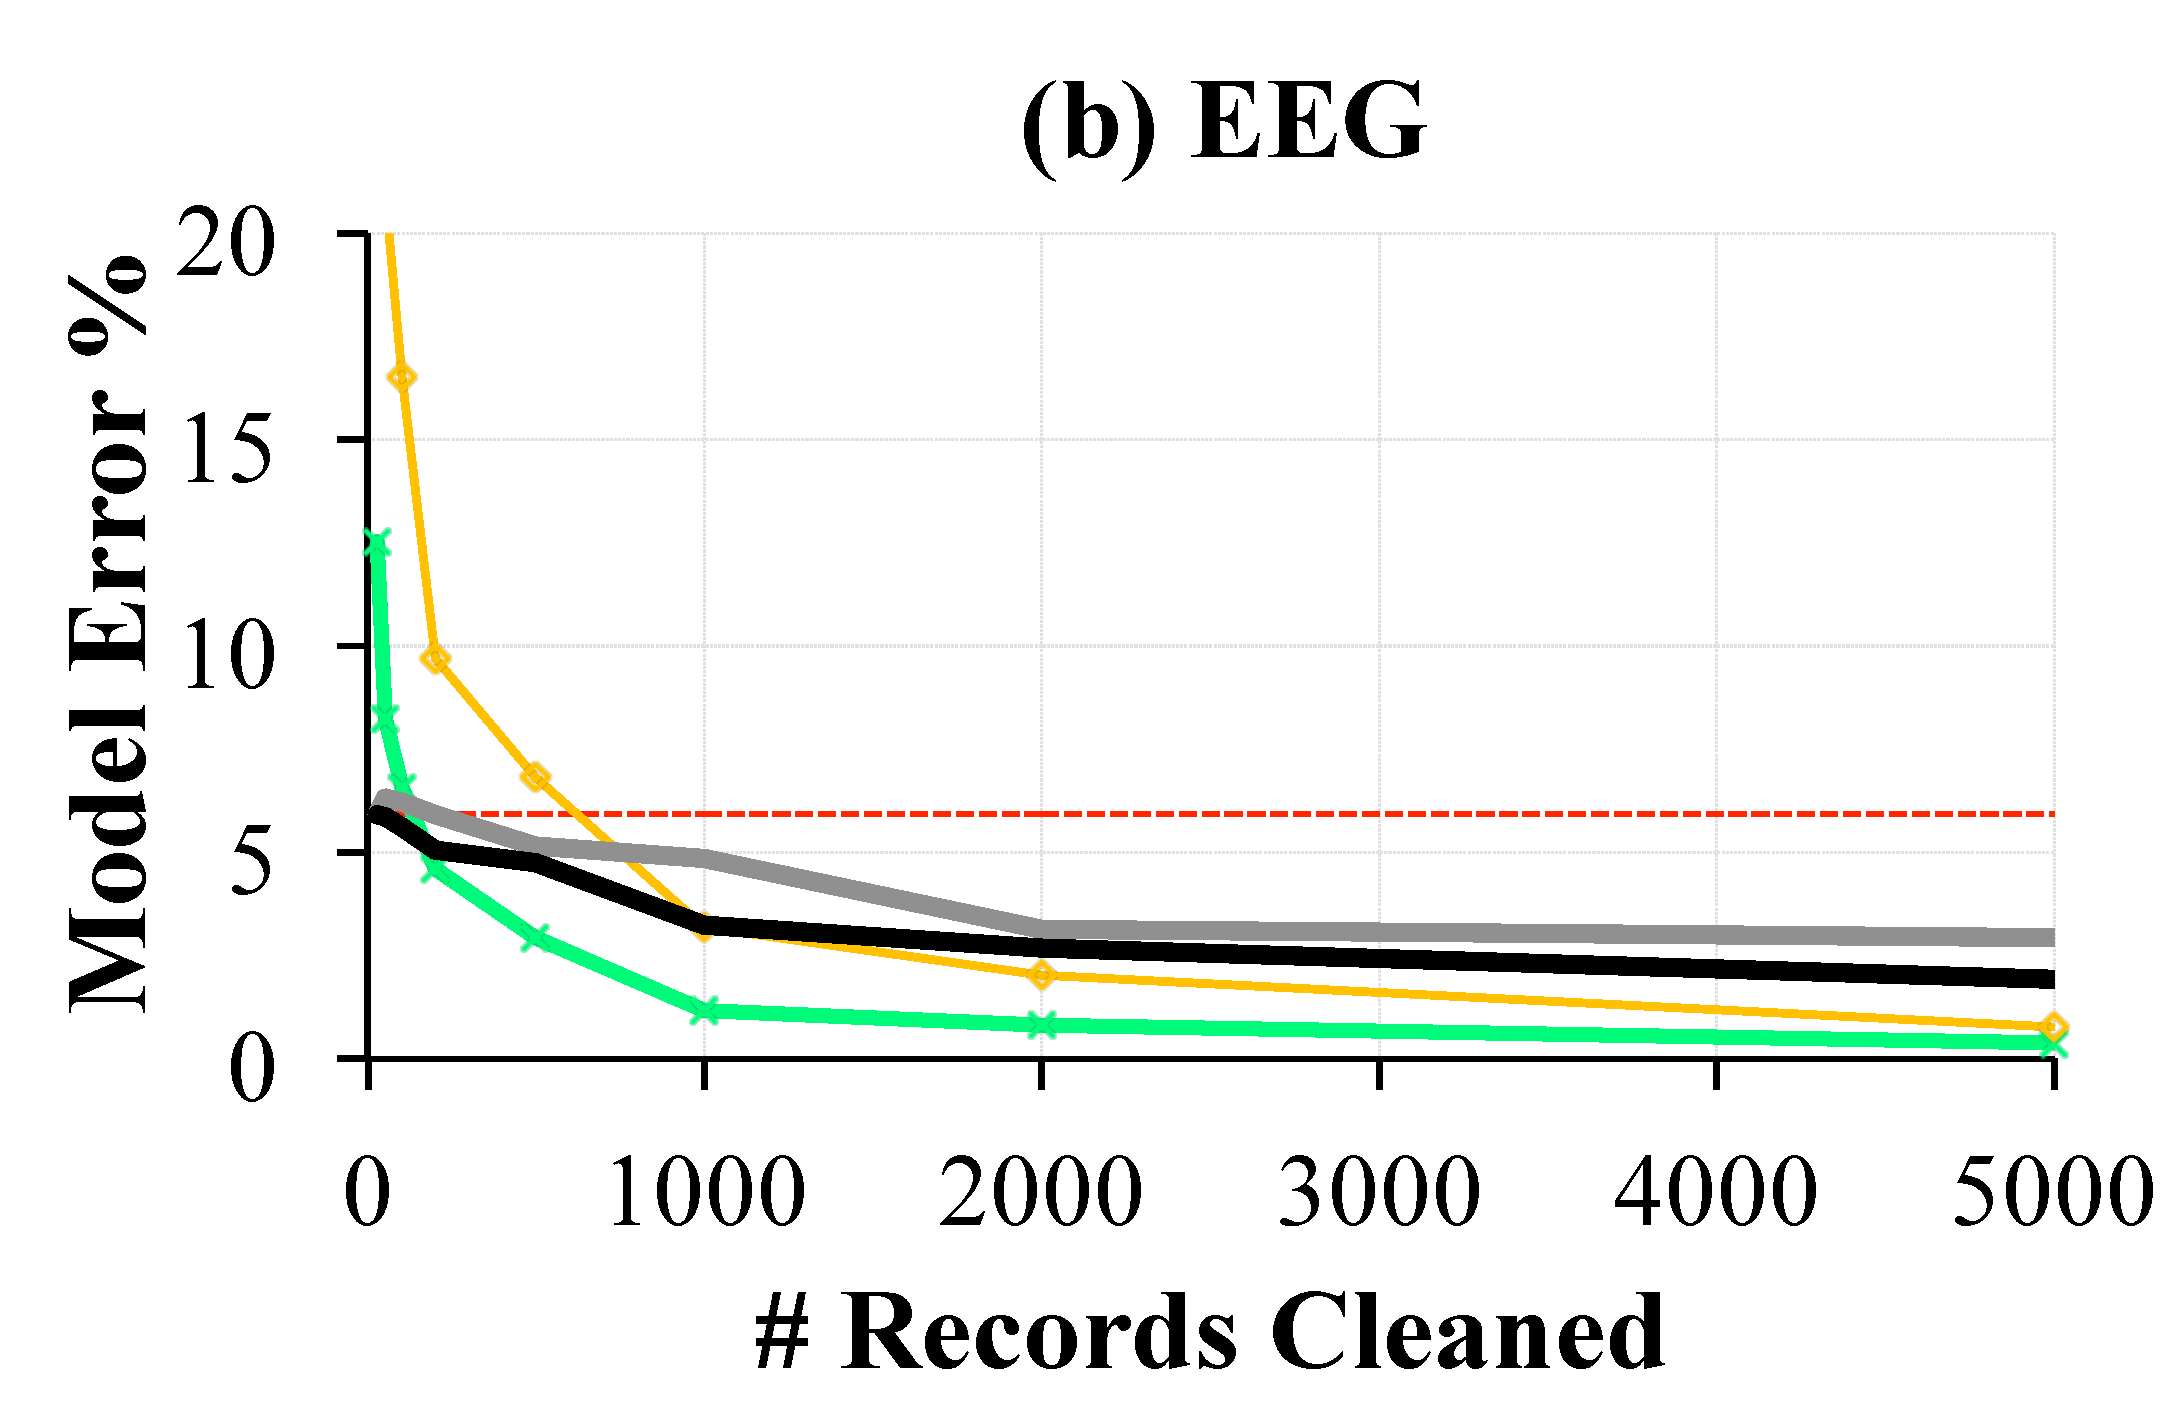
\includegraphics[width=0.49\columnwidth]{exp/exp14b.pdf}
    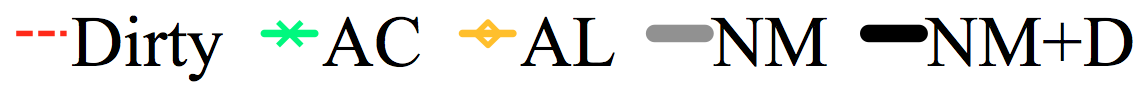
\includegraphics[width=0.49\columnwidth]{exp/legend-14.png}
 \caption{The relative model error as a function of the number of examples cleaned. \sys converges with a smaller sample size to the true result in comparison to partial cleaning (NM, NM+D).  \label{pc-perf}}
\end{figure}

\subsubsection{Corruption Rate}
This experiment explores the tradeoff between Naive-Sampling and \sys.
Figure \ref{bias} varies the systematic corruption rate and plots the number of records examined to achieve 1\% relative error for Naive-Sampling and \sys.
Naive-Sampling does not use the dirty data and thus its error is essentially governed by the the sample size and not the magnitude or prevalence of corruption.
Naive-Sampling outperforms \sys only when corruptions are very severe (45\% in Adult and nearly 60\% in EEG).
When the initialization with the dirty model is inaccurate, \sys does not perform as well. 

\begin{figure}[t]
\centering
 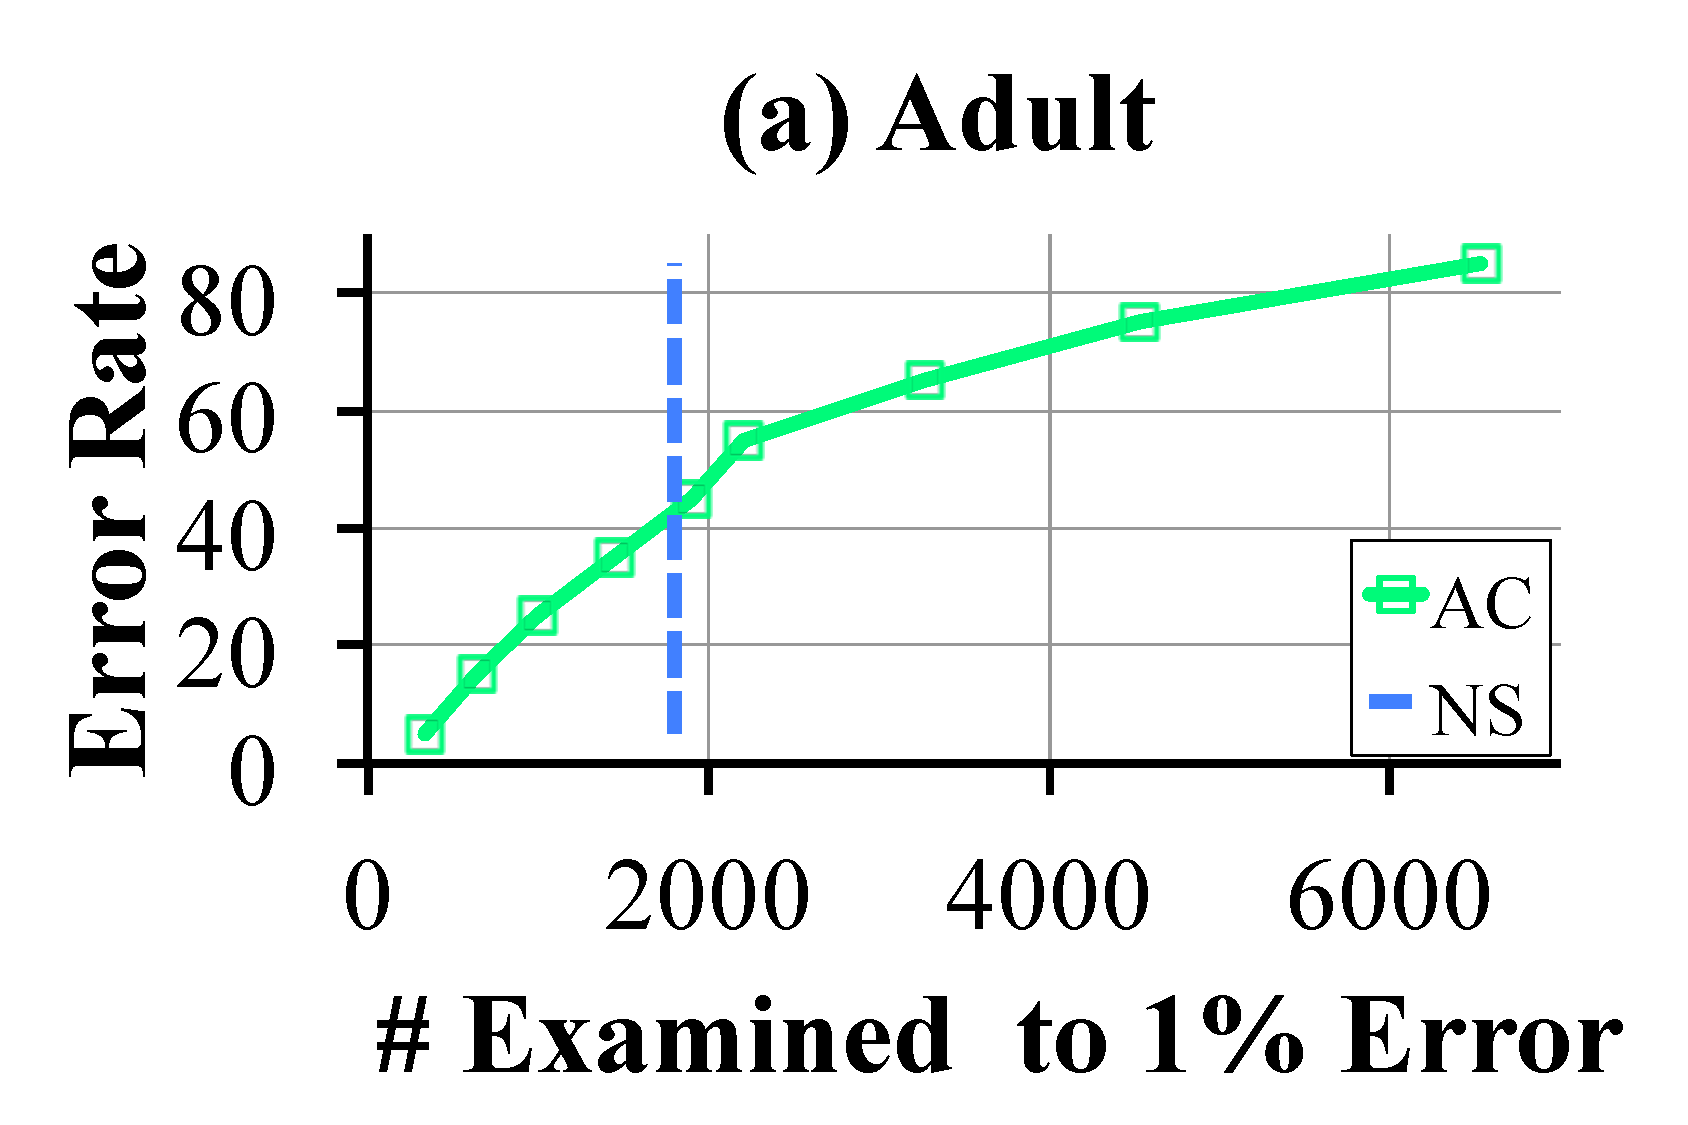
\includegraphics[width=0.49\columnwidth]{exp/exp9a.pdf}
  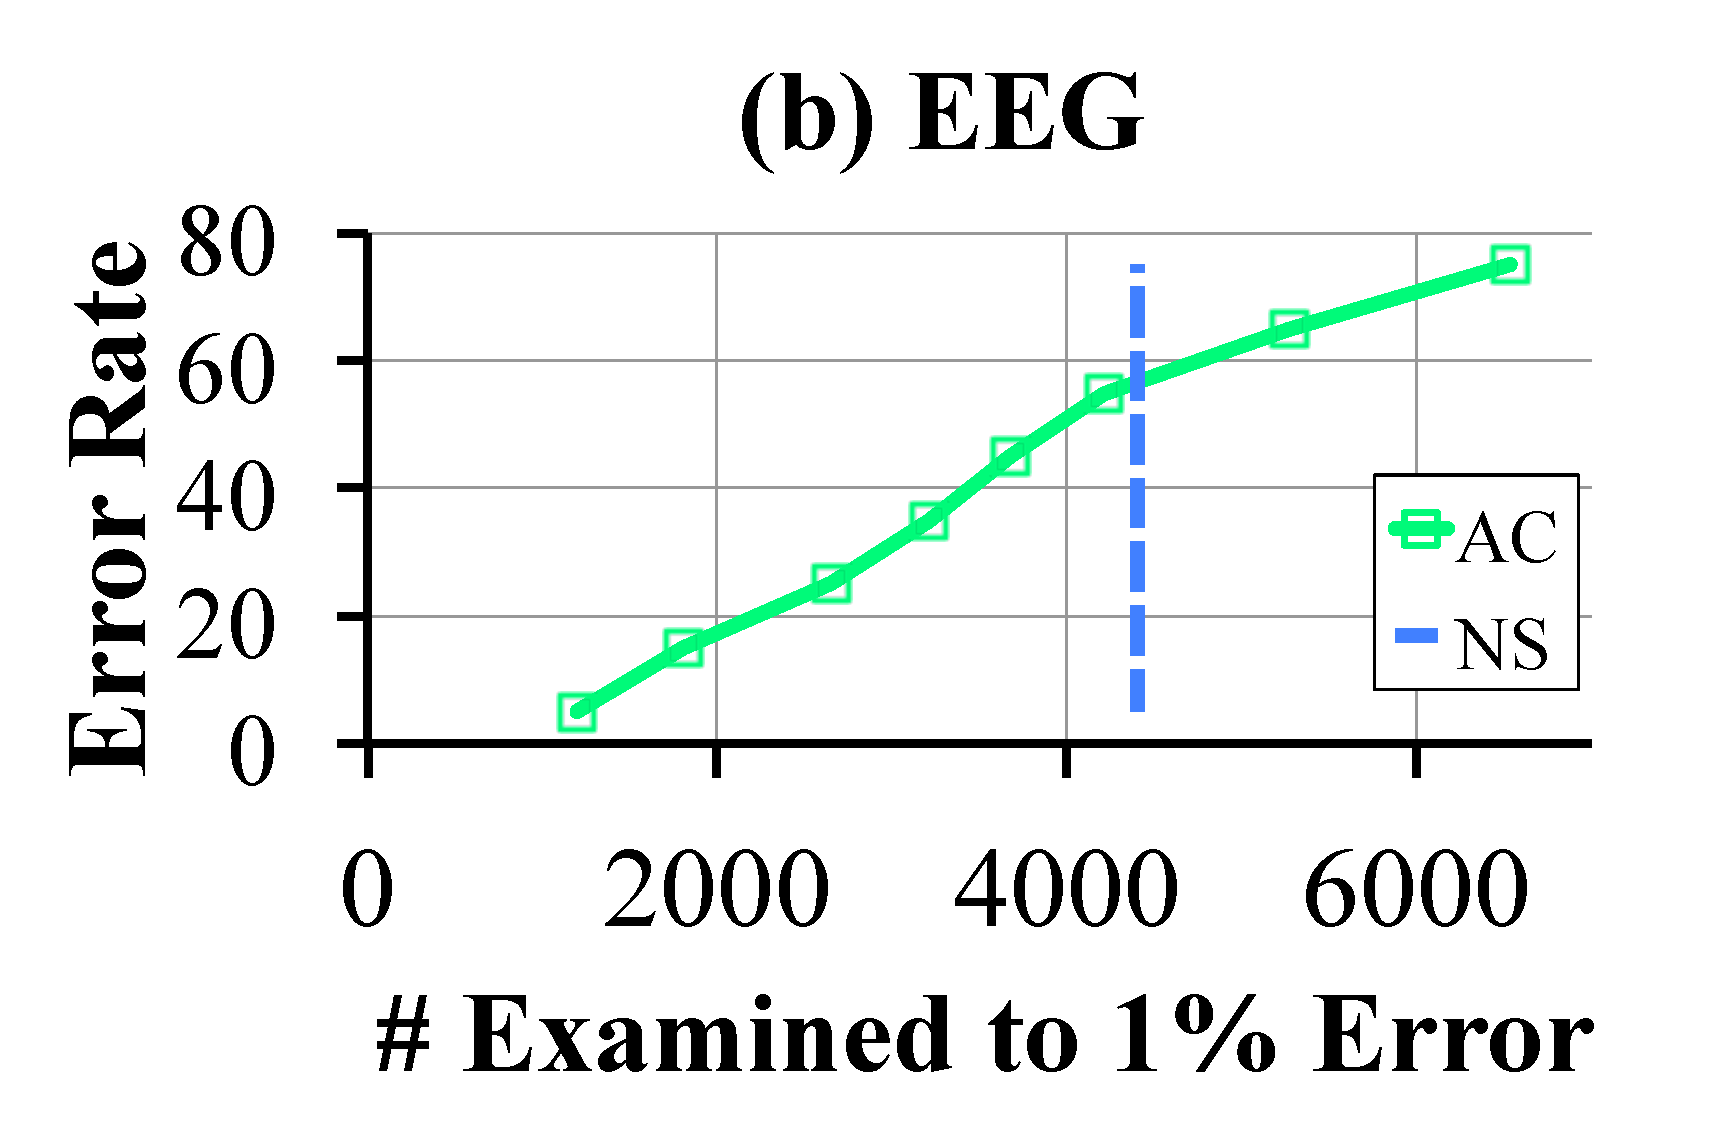
\includegraphics[width=0.49\columnwidth]{exp/exp9b.pdf}
 \caption{\sys outperforms Naive until the corruption is so severe that the dirty model is initialized very far away from the clean model.
  The error of Naive-Sampling does not depend on the corruption rate so it is a vertical line.  \label{bias}}
\end{figure}

\iffalse
\begin{figure}[t]
\centering\vspace{-1em}
 %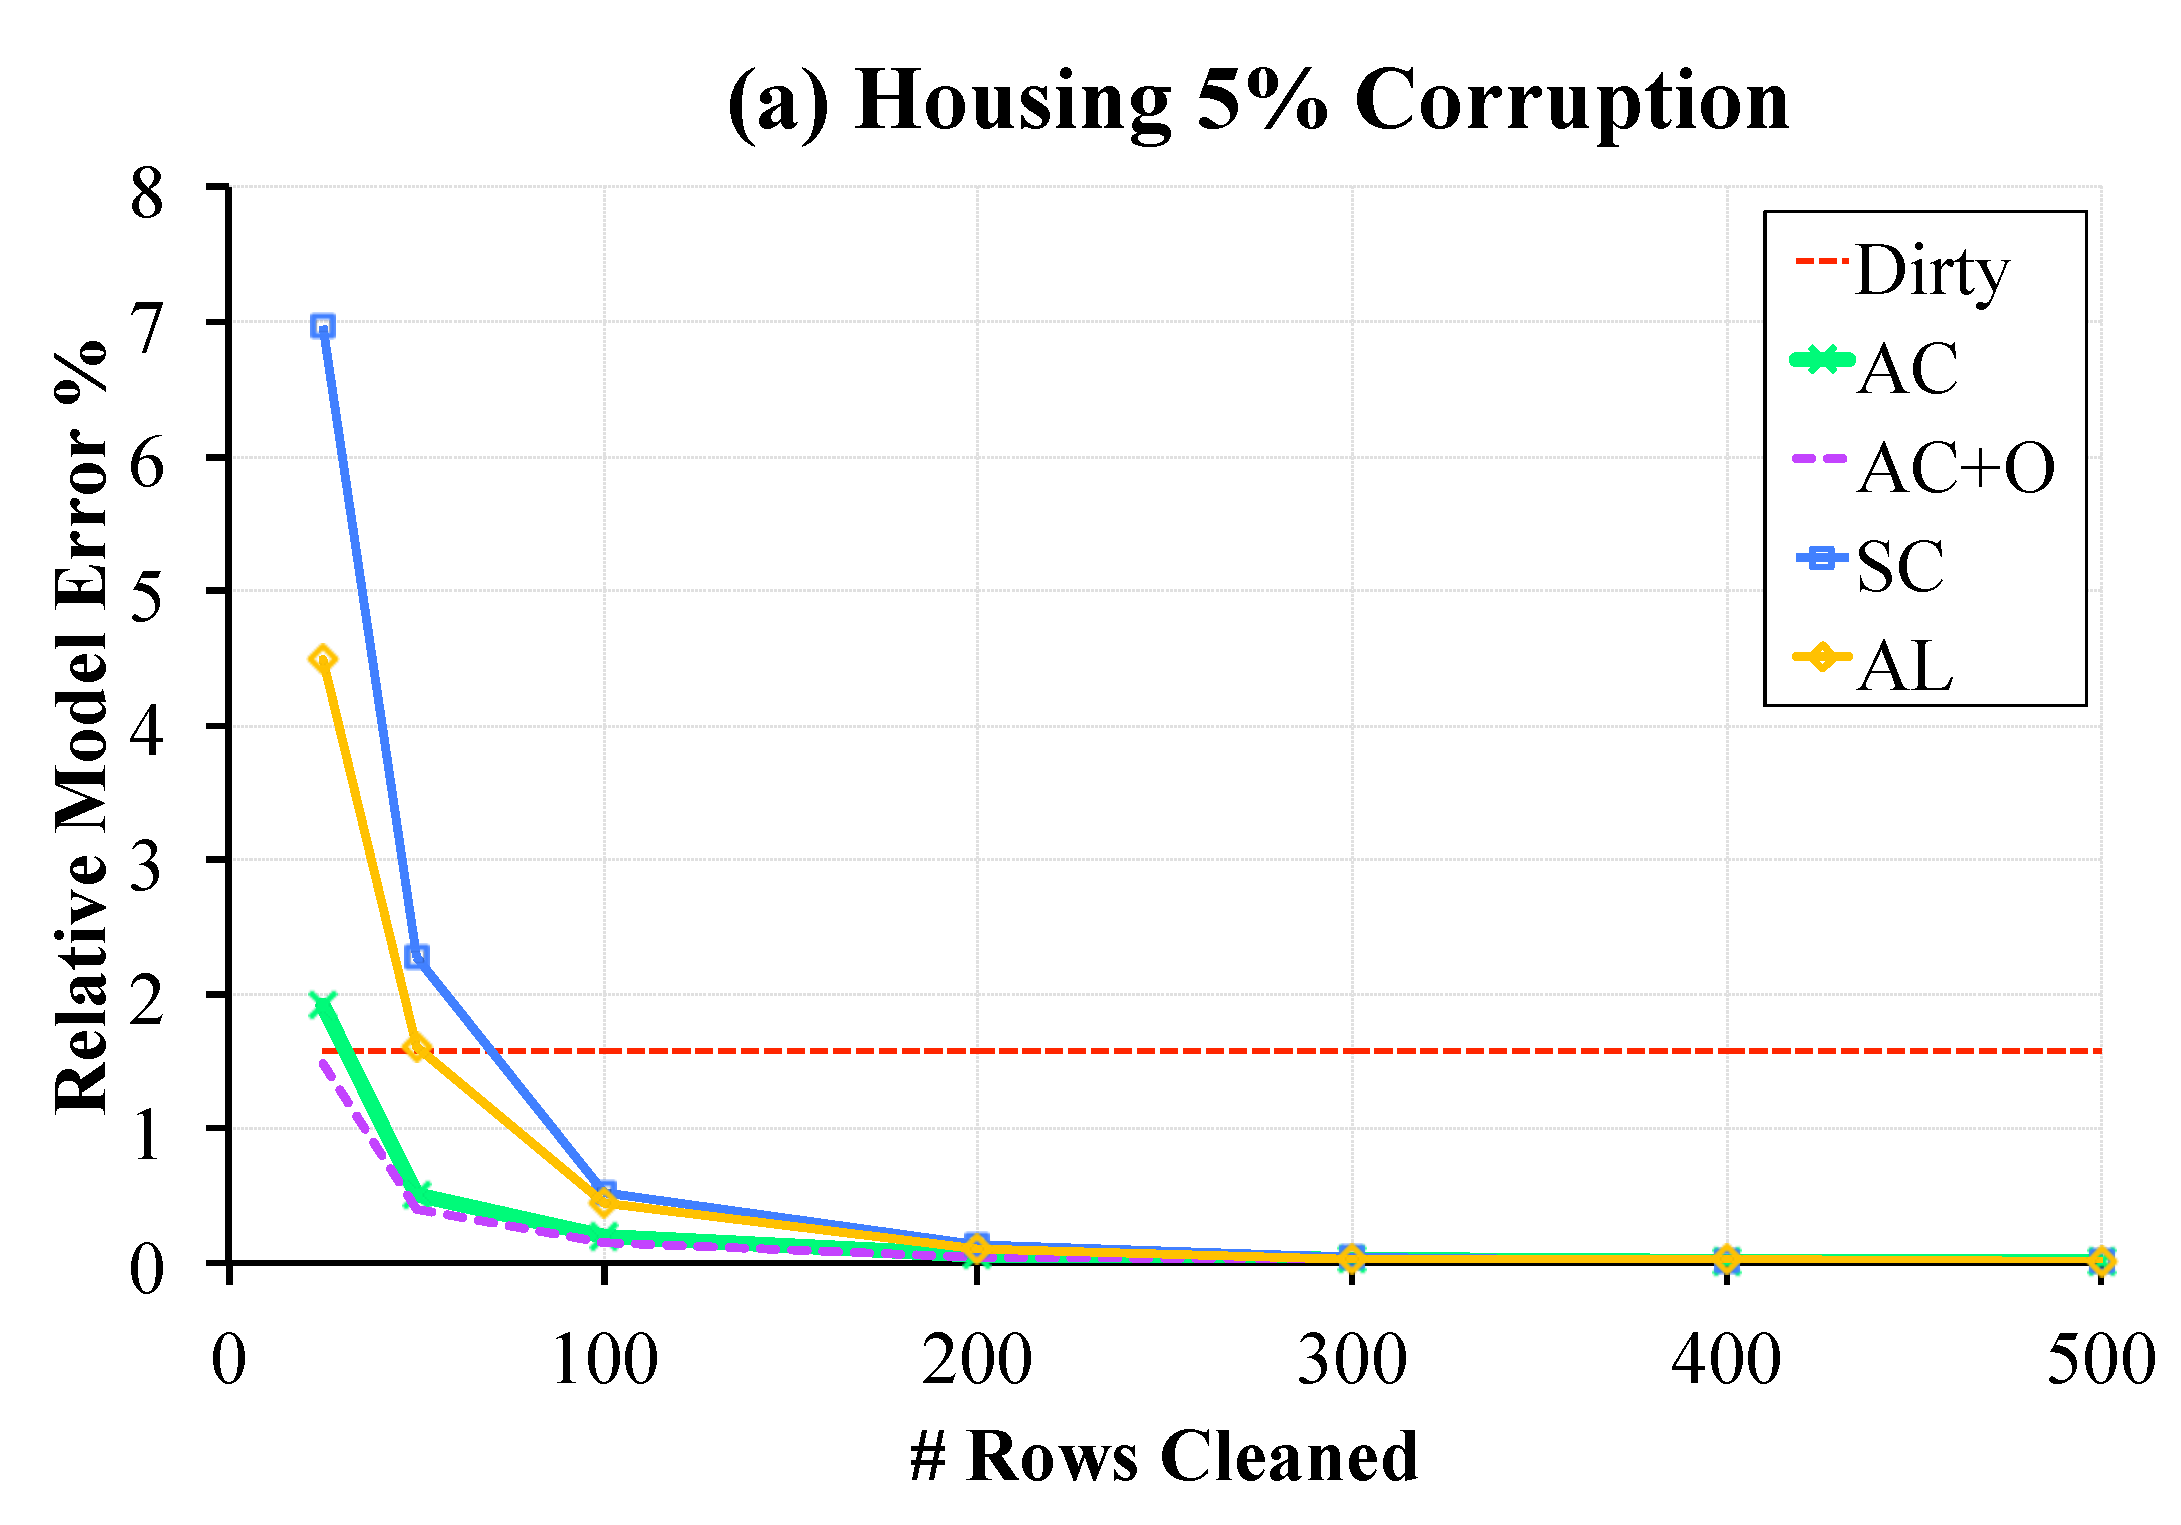
\includegraphics[scale=0.15]{exp/exp3a.pdf}
 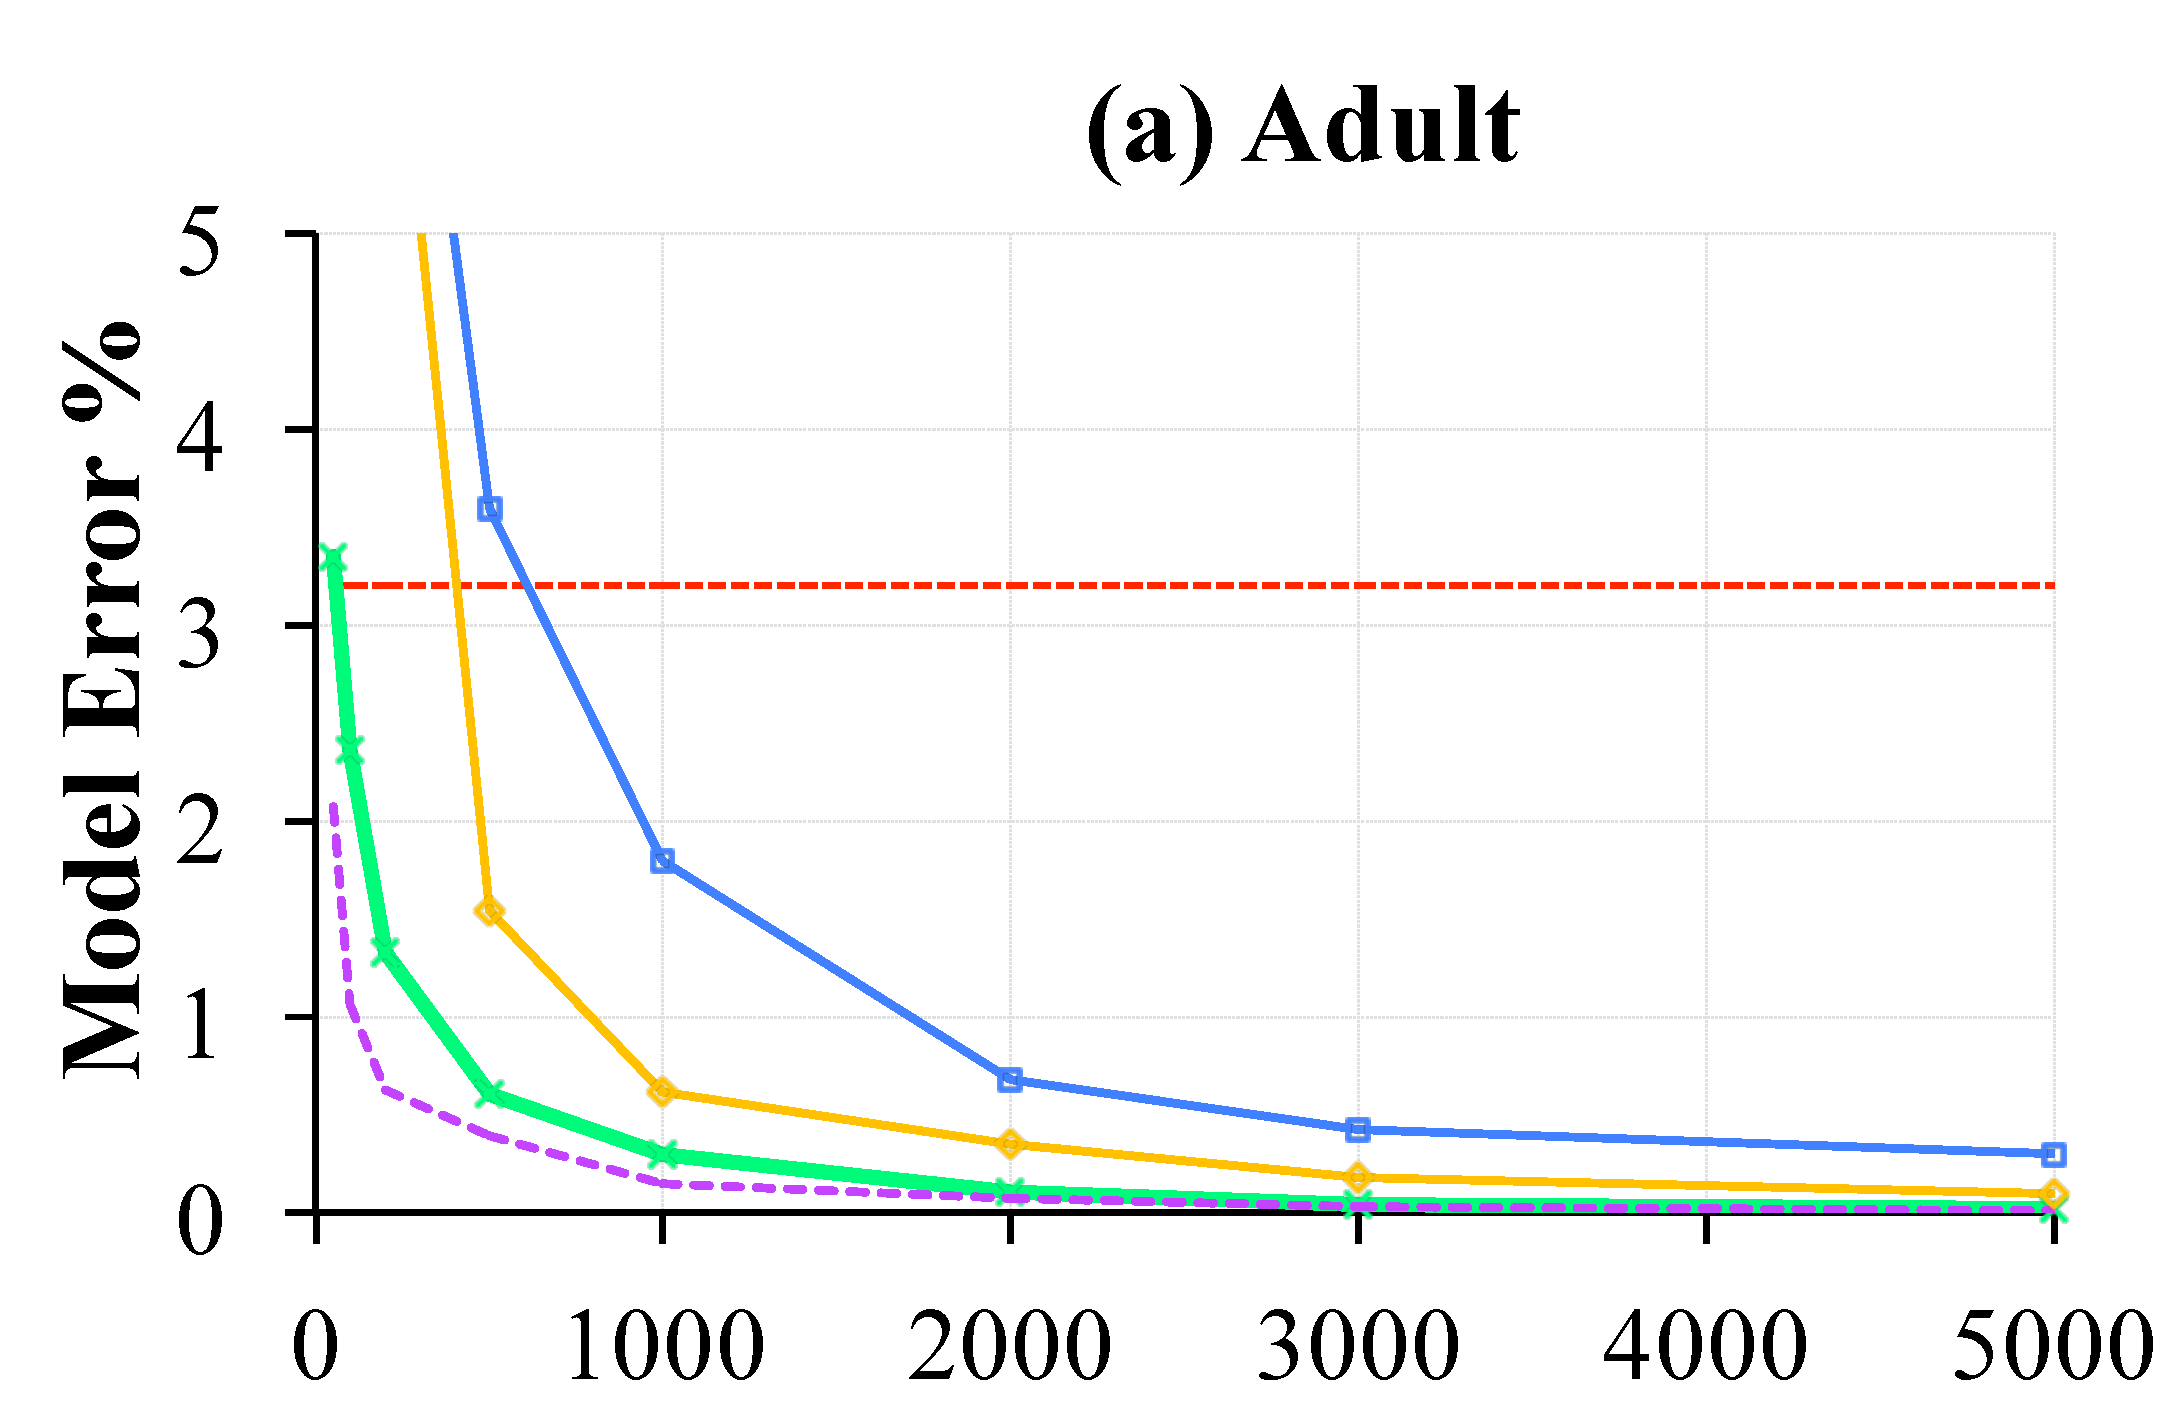
\includegraphics[width=0.49\columnwidth]{exp/exp3b.pdf}
  \includegraphics[width=0.49\columnwidth]{exp/exp3c.pdf}
  \includegraphics[width=0.49\columnwidth]{exp/exp3bb.pdf}
  \includegraphics[width=0.49\columnwidth]{exp/exp3cc.pdf}
  \includegraphics[width=0.5\columnwidth]{exp/legend-general.png}
 \caption{ The relative model error as a function of the number of examples cleaned. \sys converges with a smaller sample size to the true result in comparison to Active Learning and Naive-Sampling. \label{prio-perf}}
\end{figure}

\subsubsection{Samples-to-Error}
This experiment evaluates the samples-to-error tradeoff between four alternative algorithms: \sys (AC), SampleClean, Active Learning, and \sys+Oracle (AC+O).
Figure \ref{prio-perf} shows the model error and test accuracy as a function of the number of cleaned records.
In terms of model error, \sys gives its largest benefits for small sample sizes.
For 500 cleaned records of the Adult dataset, \sys has 6.1x less error than SampleClean and 2.1x less error than Active Learning.
For 500 cleaned records of the EEG dataset, \sys has 9.6x less error than SampleClean and 2.4x less error than Active Learning.
Both Active Learning and \sys benefit from the initialization with the dirty model as they do not retrain their models from scratch, and \sys improves on this performance with detection and error estimation.
Active Learning has no notion of dirty and clean data, and therefore prioritizes its selections with respect to the dirty data.
These gains in model error also correlate well to improvements in test error (defined as the test accuracy difference w.r.t cleaning all data).
The test error converges more quickly than model error, emphasizing the benefits of progressive data cleaning since it is not necessary to clean all the data to get a model with essentially the same performance as the clean model.
For example, to achieve a test error of 1\% on the Adult dataset, \sys cleans 500 fewer records than Active Learning.
\fi

\subsubsection{Dirty Data Detection}
Adaptive detection depends on predicting which records are dirty; and this is again related to the systematic nature of data error.
For example, random corruption not correlated with any other data features may be hard to learn.
As corruption becomes more random, the classifier becomes increasingly erroneous.
This experiment explores making our generated systematic corruption incrementally more random.
Instead of selecting the highest valued records for the most valuable features, we corrupt random records with probability $p$. 
We compare these results to AC-D where we do not have a detector at all (for a fixed number of 1000 records examined).
Figure \ref{tradeoffs2}a plots the relative error reduction using a classifier.
When the corruption is about 50\% random then there is a break even point where no detection is better.
The classifier is imperfect and misclassifies some data points incorrectly as cleaned.

\begin{figure}[t]
\centering
 \includegraphics[width=0.49\columnwidth]{exp/exp5a.pdf}
 \includegraphics[width=0.49\columnwidth]{exp/exp12.pdf}
 \caption{(a) Data corruptions that are less random are easier to classify, and lead to more significant reductions in relative model error. (b) The Taylor series approximation gives more accurate estimates when the amount of cleaned data is small. \label{tradeoffs2}}
\end{figure}

\subsubsection{Impact Estimation}\label{est}
This experiment compares estimation techniques: (1) ``linear regression" trains a linear regression model that predicts the clean gradient as a function of the dirty gradient, (2) ``average gradient" which does not use the detection to inform how to apply the estimate, (3) ``average feature change" uses detection but no linearization, and (4) the Taylor series linear approximation.
Figure \ref{tradeoffs2}b measures how accurately each estimation technique estimates the gradient as a function of the number of examined records on the EEG dataset.
Estimation error is measured using the relative L2 error with the true gradient.
The Taylor series approximation proposed gives more accurate for small cleaning sizes.

\iffalse
\subsection{Summary of Experiments}
In summary, we evaluated \sys on five datasets with both real and synthetic corruption. We find that when data error is systematic \sys can train models with a fraction of the cleaning effort of alternative techniques.
On the two real datasets, from IMDB and ProPublica, we found that many types of corruption are indeed systematic.
We also showed that our proposed optimizations (detection and sampling) further reduce cleaning effort by up-to 2.5x, and we characterized the limitations of \sys (a model trained on the dirty data is a poor initialization).
We have been noted this in our prior work on other datasets as well, where corruption is correlated with the hypotheses of interest~(see Microsoft Academic Search in~\cite{wang1999sample}, see World Bank in~\cite{activecleanarxiv}). 
However, it is possible that some types of errors do not have a systematic bias; however, the analyst could not know this for certain without applying a tool like \sys.
\fi


%\section{Conclusion}
The growing popularity of predictive models in data analytics adds additional challenges in managing dirty data.
We propose \sys, a model training framework that allows for iterative data cleaning while preserving provable convergence properties.
We specifically focus on problems that arise when data error is systematic, i.e., correlated with the hypotheses of interest.
The key insight of \sys is that convex loss models (e.g., linear regression and SVMs) can be simultaneously trained and cleaned.
%Consequently, there are provable guarantees on the convergence and error bounds of \sys.  
\sys also includes numerous optimizations such as: using the information from the model to inform data cleaning on samples, dirty data detection to avoid sampling clean data, and batching updates.
The experimental results are promising as they suggest that these optimizations can significantly reduce data cleaning costs when errors are sparse and cleaning budgets are small.
Techniques such as Active Learning and SampleClean are not optimized for the sparse low-budget setting, and \sys achieves models of high accuracy for significantly less records cleaned.

\vspace{0.5em}

\textbf{\small This research is supported in part by DHS Award HSHQDC-16-3-00083, NSF CISE Expeditions Award CCF-1139158, DOE Award SN10040 DE-SC0012463, an SFU President’s Research Start-up Grant (NO.
877335), and DARPA XData Award FA8750-12-2-0331, and gifts from Amazon Web Services, Google, IBM, SAP, The Thomas and Stacey Siebel Foundation, Apple Inc., Arimo, Blue Goji, Bosch, Cisco, Cray, Cloudera, Ericsson, Facebook, Fujitsu, HP, Huawei, Intel, Microsoft, Pivotal, Samsung, Schlumberger, Splunk, State Farm and VMware.}

%\bibliographystyle{abbrv}
%\scriptsize
\fontsize{8.0pt}{9.5pt} \selectfont
\bibliographystyle{abbrv}
\bibliography{ref} 
\normalsize \selectfont
%\appendix
%%\section{Appendix}
\section{Set-of-Records Cleaning Model}\label{set-of-r}
In paper, we formalized the analyst-specified data cleaning as follows.
We take the sample of the records $S_{dirty}$, and apply data cleaning $C(\cdot)$.
$C$ is applied to a record and produces the clean record:
\[
S_{clean} = \{C(r) : \forall r \in S_{dirty}\}
\]
The record-by-record cleaning model is a formalization of the costs of data cleaning where each record has the same cost to clean and this cost does not change throughout the entire cleaning session.
There are, however, some cases when cleaning the first record of a certain type of corruption is expensive but all subsequent records are cheaper.

\begin{example}\label{app-ex1}
In most spell checking systems, when a misspelling is identified, the system gives an option to fix all instances of that misspelling.
\end{example}

\begin{example}\label{app-ex2}
When an inconsistent value is identified all other records with the same inconsistency can be efficiently fixed.
\end{example}

This model of data cleaning can fit into our framework and we formalize it as the ``Set-of-Records" model as opposed to the ``Record-by-Record" model. 
In this model, the cleaning function $C(\cdot)$ is not restricted to updating only the records in the sample.
$C(\cdot)$ takes the entire dirty sample as an argument (that is the cleaning is a function of the sample), the dirty data, and updates the entire dirty data:
\[
R'_{dirty} = C(S_{dirty},R_{dirty})
\]
we require that for every record $s \in S_{dirty}$, that record is completely cleaned after applying $C(\cdot)$, giving us $S_{clean}$.
Records outside of $S_{dirty}$ may be cleaned on a subset of dirty attributes by $C(\cdot)$.
After each iteration, we re-run the detector, and move any $r \in R'_{dirty}$ that are clean to $R_{clean}$.
Such a model allows us to capture data cleaning operations such as in Example \ref{app-ex1} and Example \ref{app-ex2}.

\section{Stochastic Gradient Descent}\label{appsgd}

Stochastic Gradient Descent converges for a suitably chosen step size if the sample gradients are unbiased estimates of the full gradient. 
The first problem is to choose weights $\alpha$ and $\beta$ (to average already clean and newly cleaned data) such that the estimate of the gradient is unbiased. 
%SGD will converge when the estimate is unbiased and the step-size is chosen appropriately.
The batch $S_{dirty}$ is drawn only from $R_{dirty}$.
Since the sizes of $R_{dirty}$ and its complement are known, it follows that the gradient over the already clean data $g_C$ and the recently cleaned data $g_S$ can be combined as follows:
\[
g(\theta^{t}) = \frac{\mid R_{dirty} \mid \cdot g_S + \mid R_{clean} \mid \cdot g_C  }{\mid R \mid}
\]
Therefore,
\[
\alpha = \frac{\mid R_{clean} \mid}{\mid R \mid}, \beta = \frac{\mid R_{dirty} \mid}{\mid R \mid}
\]

\begin{lemma}
The gradient estimate $g(\theta)$ is unbiased if $g_S$ is an unbiased estimate of:
\[
\frac{1}{\mid R_{dirty} \mid} \sum g_i(\theta)
\]
\end{lemma}
\begin{proof}[Sketch]
\[
\mathbb{E}(\frac{1}{\mid R_{dirty} \mid} \sum g_i(\theta)) = \frac{1}{\mid R_{dirty} \mid} \cdot \mathbb{E}(\sum g_i(\theta)))
\]
By symmetry, 
\[
\mathbb{E}(\frac{1}{\mid R_{dirty} \mid} \sum g_i(\theta)) = g(\theta)
\]
\[
\mathbb{E}(\frac{1}{\mid R_{dirty} \mid} \sum g_i(\theta)) = \frac{\mid R_{dirty} \mid \cdot g_S + \mid R_{clean} \mid \cdot g_C  }{\mid R \mid}
\]
\end{proof}

The error bound discussed in Proposition 2 can be tightened for a class of models called strongly convex (see \cite{bertsekas2011incremental} for a defintion). 

\begin{proposition}
For a strongly convex loss, a batch size $b$, and $T$ iterations, the convergence rate is bounded by $O(\frac{\sigma^2}{bT})$. 
\end{proposition}

\section{Non-convex losses}\label{non-convex}
We acknowledge that there is an increasing popularity of non-convex losses in the Neural Network and Deep Learning literature. 
However, even for these losses, gradient descent techniques still apply. 
Instead of converging to a global optimum they converge to a locally optimal value. 
Likewise, \sys will converge to the closest locally optimal value to the dirty model. 
Because of this, it is harder to reason about the results.
Different initializations will lead to different local optima, and thus, introduces a complex dependence on the initialization with the dirty model.
This problem is not fundemental to \sys and any gradient technique suffers this challenge for general non-convex losses, and we hope to explore this more in the future.

\section{Importance Sampling}\label{impsample-deriv}
This lemma describes the optimal distribution over a set of scalars:
\begin{lemma}\label{impsample}
Given a set of real numbers $A = \{a_1,...,a_n\}$, let $\hat{A}$ be 
a sample with replacement of $A$ of size k.
If $\mu$ is the mean $\hat{A}$, the sampling distribution that minimizes
 the variance of $\mu$, i.e., the expected square error, is $p(a_i) \propto a_i$.
\end{lemma}
Lemma \ref{impsample} shows that when estimating a mean of numbers with sampling, the distribution with optimal variance is sampling proportionally to the values.

The variance of this estimate is given by:
\[
Var(\mu) = \mathbb{E}(\mu^2)-\mathbb{E}(\mu)^2
\] 
Since the estimate is unbiased, we can replace $\mathbb{E}(\mu)$ with the average of $A$:
\[
Var(\mu) = \mathbb{E}(\mu^2)-\bar{A}^2
\]
Since $\bar{A}$ is deterministic, we can remove that term during minimization.
Furthermore, we can write $\mathbb{E}(\mu^2)$ as:
\[
\mathbb{E}(\mu^2) = \frac{1}{n^2}\sum_i^n \frac{a_i^2}{p_i}
\]
Then, we can solve the following optimization problem (removing the proportionality of $\frac{1}{n^2}$) over the set of weights $P=\{p(a_i)\}$:
\[
\min_{P} \sum_i^N \frac{a_i^2}{p_i}
\]
\[
\text{subject to: } P > 0, \sum P = 1
\]
Applying Lagrange multipliers, an equivalent unconstrained optimization problem is:
\[
\min_{P > 0,\lambda > 0} \sum_i^N \frac{a_i^2}{p_i} + \lambda \cdot (\sum P - 1)
\]
If, we take the derivatives with respect to $p_i$ and set them equal to zero:
\[
-\frac{a_i^2}{2 \cdot p_i^2} + \lambda = 0
\]
If, we take the derivative with respect to $\lambda$ and set it equal to zero:
\[
\sum P - 1
\]
Solving the system of equations, we get:
\[
p_i = \frac{\mid a_i \mid }{\sum_i \mid a_i \mid}
\]

\section{Linearization}\label{apptaylor}
If $d$ is the dirty value and $c$ is the clean value, the Taylor series approximation for a function $f$ is given as follows:
\[
f(c) = f(d) + f'(d)\cdot(d-c) + ...
\]
Ignoring the higher order terms, the linear term $f'(d)\cdot(d-c)$ is a linear function in each feature and label.
We only have to know the change in each feature to estimate the change in value.
In our case the function $f$ is the gradient $\nabla\phi$.
So, the resulting linearization is:
\[
\nabla\phi(x^{(c)}_i,y^{(c)}_i,\theta) \approx \nabla\phi(x,y,\theta) + \frac{\partial}{\partial X}\nabla\phi(x,y,\theta)\cdot (x - x^{(c)}) \]
\[+ \frac{\partial}{\partial Y}\phi(x,y,\theta)\cdot (y - y^{(c)})
\]
When we take the expected value:
\[
\mathbb{E}(\nabla\phi(x_{clean},y_{clean},\theta)) \approx \nabla\phi(x,y,\theta) + \frac{\partial}{\partial X}\nabla\phi(x,y,\theta)\cdot \mathbb{E}(\Delta x) \]
\[+ \frac{\partial}{\partial Y}\nabla\phi(x,y,\theta)\cdot \mathbb{E}(\Delta y)
\]
It follows that:
\[
\approx \nabla\phi(x,y,\theta) + M_x \cdot \mathbb{E}(\Delta x) + M_y \cdot \mathbb{E}(\Delta y)
\]
where $M_x = \frac{\partial}{\partial X}\nabla\phi$ and $M_y = \frac{\partial}{\partial Y}\nabla\phi$.
Recall that the feature space is $d$ dimensional and label space is $l$ dimensional.
Then, $M_x$ is an $d \times d$ matrix, and $M_y$ is a $d \times l$ matrix.
Both of these matrices are computed for each record.
$\Delta x$ is a $d$ dimensional vector where each component represents a change in that feature and $\Delta y$ is an $l$ dimensional vector that represents the change in each of the labels. 

This linearization allows \sys to maintain per feature (or label) average changes and use these changes to center the optimal sampling distribution around the expected clean value.
To estimate $\mathbb{E}(\Delta x)$ and $\mathbb{E}(\Delta y)$, consider the following for a single feature $i$:
If we average all $j=\{1,...,K\}$ records cleaned that have an error for that feature, weighted by their sampling probability:
\[
\bar{\Delta}_{xi} = \frac{1}{NK}\sum_{j=1}^K (x^{(d)}[i]-x^{(c)}[i])\times \frac{1}{p(j)}
\]
Similarly, for a label $i$:
\[
\bar{\Delta}_{yi} = \frac{1}{NK}\sum_{j=1}^K (y^{(d)}[i]-y^{(c)}[i])\times \frac{1}{p(j)}
\]

Each $\bar{\Delta}_{xi}$ and $\bar{\Delta}_{yi}$ represents an average change in a single feature.
A single vector can represent the necessary changes to apply to a record $r$:
For a record $r$, the set of corrupted features is $f_r,l_r$.
Then, each record $r$ has a d-dimensional vector $\Delta_{rx}$ which is constructed as follows:
\[
 \Delta_{rx}[i] = \begin{cases} 0 & i \notin f_r \\ 
\bar{\Delta}_{xi} & i \in f_r
\end{cases} 
\]
Each record $r$ also has an l-dimensional vector $\Delta_{ry}$ which is constructed as follows:
\[
 \Delta_{rx}[i] = \begin{cases} 0 & i \notin l_r \\ 
\bar{\Delta}_{yi} & i \in l_r
\end{cases} 
\]
Finally, the result is: 
\[p_{r}\propto\|\nabla\phi(x,y,\theta^{(t)}) + M_x \cdot \Delta_{rx} +  M_y \cdot \Delta_{ry}\|
\]

\section{Example $M_x$, $M_y$}\label{example-deriv}
\noindent\textbf{Linear Regression: }
\[
\nabla\phi(x,y,\theta) = (\theta^Tx - y)x
\]
For a record, $r$, suppose we have a feature vector $x$.
If we take the partial derivatives with respect to x, $M_x$ is:
\[
M_x[i,i] = 2x[i] + \sum_{i \ne j} \theta[j]x[j] - y 
\]
\[
M_x[i,j] = \theta[j]x[i]
\]
Similarly $M_y$ is:
\[
M_y[i,1] = x[i] 
\]

\vspace{0.5em}

\noindent\textbf{Logistic Regression: } 
\[
\nabla\phi(x,y,\theta) = (h(\theta^Tx) - y)x
\]
where
\[
h(z) = \frac{1}{1+e^{-z}}
\]
we can rewrite this as:
\[
h_{\theta}(x) = \frac{1}{1+e^{\theta^Tx}}
\]
\[
\nabla\phi(x,y,\theta) = (h_{\theta}(x) - y)x
\]
In component form,
\[
g = \nabla\phi(x,y,\theta)
\]
\[
g[i] = h_{\theta}(x)\cdot x[i] - yx[i]
\]
Therefore,
\[
M_x[i,i] = h_{\theta}(x)\cdot(1- h_{\theta}(x))\cdot \theta[i] x[i] + h_{\theta}(x) - y
\]
\[
M_x[i,j] = h_{\theta}(x)\cdot(1- h_{\theta}(x))\cdot \theta[j] x[i] + h_{\theta}(x)
\]
\[
M_y[i,1] = x[i] 
\]

\noindent\textbf{SVM: } 
\[
\nabla\phi(x,y,\theta) =
\begin{cases}      
-y\cdot\boldsymbol{x} \text{ if } y\cdot\boldsymbol{x}\cdot\theta \le 1 \\
0\ \text{ if } y\ \boldsymbol{x}\cdot\theta \geq 1      
\end{cases}
\]
Therefore,
\[
M_x[i,i] = \begin{cases}      
-y[i] \text{ if } y\cdot\boldsymbol{x}\cdot\theta \le 1 \\
0\ \text{ if } y\ \boldsymbol{x}\cdot\theta \geq 1      
\end{cases} 
\]
\[
M_x[i,j] = 0
\]
\[
M_y[i,1] = x[i] 
\]

\section{Aggregate Queries as \\ Convex Losses}
\subsection{AVG and SUM queries}
\avgfunc, \sumfunc queries are a special case of the convex loss minimization discussed in the paper:
If we define the following loss, it is easy to verify the the optimal $\theta$ is the mean $\mu$:
\[
\phi = (x_{i} - \theta)^2
\]
with the appropriate scaling it can support $\avgfunc$, $\sumfunc$ queries with and without predicates.
Taking the gradient of that loss:
\[
\nabla\phi = 2(x_{i} - \theta)
\]
It is also easy to verify that the bound on errors is $O(\frac{\mathbb{E}((x-\mu)^2}{bT})$, which is essentially the CLT.
The importance sampling results are inutitive as well.
Applying the linearization:
\[
M_x = 2
\]
The importance sampling prioritizes points that it expects to be far away from the mean.

\subsection{MEDIAN}
Similarly, we can analyze the \medfunc query.
If we define the following loss, it is easy to verify the the optimal $\theta$ is the median $m$:
\[
\phi = \mid x_{i} - \theta\mid
\]
Taking the gradient of that loss:
\[
\nabla\phi = \text{1 if < m, -1 if > m}
\]
Applying the linearization:
\[
M_x = 0
\]
The intuitive result is that a robust query like a median does not need to consider estimation as the query result is robust to small changes.

\section{Experimental Comparison}
\subsection{Robust Logistic Regression}\label{rlogit}
We use the algorithm from Feng et al. for robust logistic regression.
\begin{enumerate}
\item Input: Contaminated training samples $\{(x_1, y_1), . . . ,(x_{n}
, y_{n})\}$ an upper bound on the number of outliers n, number of inliers n and sample dimension p.
\item Initialization: Set \[T = 4\sqrt{\log p/n + \log n/n}\]
\item Remove samples $(xi
, yi)$ whose magnitude satisfies $\|x_i\| \ge T$.
\item Solve regularized logistic regression problem.
\end{enumerate}

\section{Dollars For Docs Setup}\label{dfd-errors}
The dollars for docs dataset has the following schema:
\begin{lstlisting}[mathescape,basicstyle={\scriptsize}]
Contribution(pi_speciality$\textrm{,}$ drug_name$\textrm{,}$ device_name$\textrm{,}$
corporation$\textrm{,}$ amount$\textrm{,}$ dispute$\textrm{,}$ status)
\end{lstlisting}
To flag suspect donations, we used the \texttt{status} attribute.
When the \texttt{status} was ``covered" that means it was an allowed contribution under the researcher's declared protocol.
When the \texttt{status} was ``non-covered" that means it was a disallowed contribution under the researcher's declared protocol.
The rest of the textual attributes were featurized with a bag-of-words model, and the numerical amount and dispute attributes were treated as numbers.

We cleaned the entire Dollars for Docs dataset upfront to be able to evaluate how different budgeted data cleaning strategies compare to cleaning the full data.
To clean the dataset, we loaded the entire data 240089 records into Microsoft Excel. We identified four broad classes of errors:
\vspace{0.25em}

\noindent \textbf{Corporations are inconsistently represented: } ``Pfizer", ``Pfizer Inc.", ``Pfizer Incorporated".

\vspace{0.25em}

\noindent \textbf{Drugs are inconsistently represented: } ``TAXOTERE  DOCETAXEL -PROSTATE CANCER" and ``TAXOTERE"

\vspace{0.25em}

\noindent \textbf{Label of covered and not covered are not consistent: } ``No", ``Yes",``N", ``This study is not supported", ``None", ``Combination"

\vspace{0.25em} 

\noindent \textbf{Research subject must be a drug OR a medical device and not both: } ``BIO FLU QPAN H7N9AS03 Vaccine" and ``BIO FLU QPAN H7N9AS03 Device"

\vspace{0.5em} 

To fix these errors, we sorted by each column and merged values that looked similar and removed inconsistencies as in the status labels. 
When there were ambiguities, we refered to the drug company's website and whitepapers.
When possible, we used batch data transformations, like find and replace (i.e. the Set-of-Records model).
In all, 44234 records had some error and full data cleaning required about 2 days of efforts.

Once cleaned, in our experiment, we encoded the 4 problems as data quality constraints.
To fix the constraints, we looked up the clean value in the dataset that we cleaned up front.

\vspace{0.25em}

\noindent \textbf{Rule 1: } Matching dependency on corporation (Weighted Jaccard Similarity $>$ 0.8).

\vspace{0.25em}

\noindent \textbf{Rule 2: } Matching dependency on drug (Weighted Jaccard Similarity $>$ 0.8).

\vspace{0.25em}

\noindent \textbf{Rule 3: } Label must either be ``covered" or ``not covered".

\vspace{0.25em} 

\noindent \textbf{Rule 4: } Either drug or medical device should be null.

\vspace{0.5em}

\section{MNIST Setup}
We include visualization of the errors that we generated for the MNIST experiment.
We generated these errors in MATLAB by taking the grayscale version of the image (a $64\times 64$ matrix) and corrupting them by block removal and fuzzying.

\begin{figure}[ht]
\centering
\includegraphics[scale=0.20]{exp/original.png}
 \includegraphics[scale=0.20]{exp/5x5removal.png}
 \includegraphics[scale=0.20]{exp/fuzzy.png}
 \caption{We experiment with two forms of corruption in the MNIST image datasets: 5x5 block removal and making the images fuzzy. Image (a) shows an uncorrupted ``9", image (b) shows one corrupted with block removal, and image (c) shows one that is corrupted with fuzziness. \label{mnist-corr}}
\end{figure}

\end{document}
